%DIF 1a1-6
%DIF LATEXDIFF DIFFERENCE FILE
%DIF DEL old.tex   Sun Oct 30 15:57:22 2022
%DIF ADD new.tex   Mon Jul 31 11:08:26 2023
 %DIF > 
%% ---------------------------------
 %DIF > 
%% This template should be used for copernicus.cls
 %DIF > 
%% The class file and some style files are bundled in the Copernicus Latex Package, which can be downloaded from the different journal webpages.
 %DIF > 
%% For further assistance please contact Copernicus Publications at: production@copernicus.org
 %DIF > 
%% https://publications.copernicus.org/for_authors/manuscript_preparation.html
 %DIF > 
%DIF -------





%DIF PREAMBLE EXTENSION ADDED BY LATEXDIFF
%DIF UNDERLINE PREAMBLE %DIF PREAMBLE
\RequirePackage[normalem]{ulem} %DIF PREAMBLE
\RequirePackage{color}\definecolor{RED}{rgb}{1,0,0}\definecolor{BLUE}{rgb}{0,0,1} %DIF PREAMBLE
\providecommand{\DIFadd}[1]{{\protect\color{blue}\uwave{#1}}} %DIF PREAMBLE
\providecommand{\DIFdel}[1]{{\protect\color{red}\sout{#1}}}                      %DIF PREAMBLE
%DIF SAFE PREAMBLE %DIF PREAMBLE
\providecommand{\DIFaddbegin}{} %DIF PREAMBLE
\providecommand{\DIFaddend}{} %DIF PREAMBLE
\providecommand{\DIFdelbegin}{} %DIF PREAMBLE
\providecommand{\DIFdelend}{} %DIF PREAMBLE
%DIF FLOATSAFE PREAMBLE %DIF PREAMBLE
\providecommand{\DIFaddFL}[1]{\DIFadd{#1}} %DIF PREAMBLE
\providecommand{\DIFdelFL}[1]{\DIFdel{#1}} %DIF PREAMBLE
\providecommand{\DIFaddbeginFL}{} %DIF PREAMBLE
\providecommand{\DIFaddendFL}{} %DIF PREAMBLE
\providecommand{\DIFdelbeginFL}{} %DIF PREAMBLE
\providecommand{\DIFdelendFL}{} %DIF PREAMBLE
%DIF END PREAMBLE EXTENSION ADDED BY LATEXDIFF






%DIF 2-14d8
%DIF < \documentclass[twocolumn]{article}
%DIF < \usepackage[english]{babel}
%DIF < \usepackage[utf8]{inputenc}
%DIF < \usepackage{amsmath}
%DIF < \usepackage{centernot}
%DIF < \usepackage{amsfonts}
%DIF < \usepackage{subcaption}
%DIF < \usepackage{mathtools}
%DIF < \usepackage{graphicx}
%DIF < \usepackage{color}
%DIF < \usepackage{authblk}
%DIF < \usepackage{url}
%DIF < \usepackage{amssymb}
%DIF -------

%DIF 16a9
%% Please use the following documentclass and journal abbreviations for preprints and final revised papers.
 %DIF > 
%DIF -------

%DIF 17-19c11-12
%DIF < \usepackage[colorlinks,citecolor=blue,linkcolor=blue,urlcolor=blue,bookmarks=false,hypertexnames=true]{hyperref}
%DIF < \usepackage{geometry}
%DIF < \graphicspath{{images/}}
%DIF -------
%% 2-column papers and preprints
 %DIF > 
\documentclass[hess, twostagejnl]{copernicus}
 %DIF > 
%DIF -------
%DIF 21-29c14
%DIF < % Margins:
%DIF < \geometry{
%DIF < 	a4paper,
%DIF < 	total={170mm,257mm},
%DIF < 	left=20mm,
%DIF < 	right=20mm,
%DIF < 	top=20mm,
%DIF < 	bottom=20mm,
%DIF < }
%DIF -------
%\documentclass[tc,manuscript]{copernicus}
 %DIF > 
%DIF -------

%DIF 31c16
%DIF < \def\UrlBreaks{\do\/\do-}
%DIF -------
%% Journal abbreviations (please use the same for preprints and final revised papers)
 %DIF > 
%DIF -------

%DIF 33-45d18
%DIF < %\usepackage[ruled]{algorithm2e}
%DIF < %
%DIF < %
%DIF < %\makeatletter
%DIF < %\newcommand{\RemoveAlgoNumber}{\renewcommand{\fnum@algocf}{\AlCapSty{\AlCapFnt\algorithmcfname}}}
%DIF < %\newcommand{\RevertAlgoNumber}{\algocf@resetfnum}
%DIF < %\makeatother
%DIF < %
%DIF < %%\renewcommand*{\listalgorithmcfname}{List of Heuristics}
%DIF < %\renewcommand*{\algorithmcfname}{SPEEDY}
%DIF < %%\renewcommand*{\algorithmautorefname}{heuristic}
%DIF < %
%DIF < %
%DIF -------

%DIF 47a19-64
% Advances in Geosciences (adgeo)
 %DIF > 
% Advances in Radio Science (ars)
 %DIF > 
% Advances in Science and Research (asr)
 %DIF > 
% Advances in Statistical Climatology, Meteorology and Oceanography (ascmo)
 %DIF > 
% Annales Geophysicae (angeo)
 %DIF > 
% Archives Animal Breeding (aab)
 %DIF > 
% Atmospheric Chemistry and Physics (acp)
 %DIF > 
% Atmospheric Measurement Techniques (amt)
 %DIF > 
% Biogeosciences (bg)
 %DIF > 
% Climate of the Past (cp)
 %DIF > 
% DEUQUA Special Publications (deuquasp)
 %DIF > 
% Drinking Water Engineering and Science (dwes)
 %DIF > 
% Earth Surface Dynamics (esurf)
 %DIF > 
% Earth System Dynamics (esd)
 %DIF > 
% Earth System Science Data (essd)
 %DIF > 
% E&G Quaternary Science Journal (egqsj)
 %DIF > 
% EGUsphere (egusphere) | This is only for EGUsphere preprints submitted without relation to an EGU journal.
 %DIF > 
% European Journal of Mineralogy (ejm)
 %DIF > 
% Fossil Record (fr)
 %DIF > 
% Geochronology (gchron)
 %DIF > 
% Geographica Helvetica (gh)
 %DIF > 
% Geoscience Communication (gc)
 %DIF > 
% Geoscientific Instrumentation, Methods and Data Systems (gi)
 %DIF > 
% Geoscientific Model Development (gmd)
 %DIF > 
% History of Geo- and Space Sciences (hgss)
 %DIF > 
% Hydrology and Earth System Sciences (hess)
 %DIF > 
% Journal of Bone and Joint Infection (jbji)
 %DIF > 
% Journal of Micropalaeontology (jm)
 %DIF > 
% Journal of Sensors and Sensor Systems (jsss)
 %DIF > 
% Magnetic Resonance (mr)
 %DIF > 
% Mechanical Sciences (ms)
 %DIF > 
% Natural Hazards and Earth System Sciences (nhess)
 %DIF > 
% Nonlinear Processes in Geophysics (npg)
 %DIF > 
% Ocean Science (os)
 %DIF > 
% Polarforschung - Journal of the German Society for Polar Research (polf)
 %DIF > 
% Primate Biology (pb)
 %DIF > 
% Proceedings of the International Association of Hydrological Sciences (piahs)
 %DIF > 
% Safety of Nuclear Waste Disposal (sand)
 %DIF > 
% Scientific Drilling (sd)
 %DIF > 
% SOIL (soil)
 %DIF > 
% Solid Earth (se)
 %DIF > 
% State of the Planet (sp)
 %DIF > 
% The Cryosphere (tc)
 %DIF > 
% Weather and Climate Dynamics (wcd)
 %DIF > 
% Web Ecology (we)
 %DIF > 
% Wind Energy Science (wes)
 %DIF > 
%DIF -------

%DIF 48d66
%DIF < \usepackage{listings}
%DIF -------

%DIF 50-68c67-78
%DIF < \definecolor{dkgreen}{rgb}{0,0.6,0}
%DIF < \definecolor{gray}{rgb}{0.5,0.5,0.5}
%DIF < \definecolor{mauve}{rgb}{0.58,0,0.82}
%DIF < \lstset{frame=tb,
%DIF < 	language=Fortran,
%DIF < 	aboveskip=3mm,
%DIF < 	belowskip=3mm,
%DIF < 	showstringspaces=false,
%DIF < 	columns=flexible,
%DIF < 	basicstyle={\small\ttfamily},
%DIF < 	numbers=none,	
%DIF < 	numberstyle=\tiny\color{gray},
%DIF < 	keywordstyle=\color{blue},
%DIF < 	commentstyle=\color{dkgreen},
%DIF < 	stringstyle=\color{mauve},
%DIF < 	breaklines=true,
%DIF < 	breakatwhitespace=true,
%DIF < 	tabsize=3
%DIF < }
%DIF -------
%% \usepackage commands included in the copernicus.cls:
 %DIF > 
%\usepackage[german, english]{babel}
 %DIF > 
%\usepackage{tabularx}
 %DIF > 
%\usepackage{cancel}
 %DIF > 
%\usepackage{multirow}
 %DIF > 
%\usepackage{supertabular}
 %DIF > 
%\usepackage{algorithmic}
 %DIF > 
%\usepackage{algorithm}
 %DIF > 
%\usepackage{amsthm}
 %DIF > 
%\usepackage{float}
 %DIF > 
%\usepackage{subfig}
 %DIF > 
%\usepackage{rotating}
 %DIF > 
%DIF -------


%DIF 71d81
%DIF < \date{}
%DIF -------

%DIF 73a82-86
%Author added
 %DIF > 
\graphicspath{{images/}}
 %DIF > 
\usepackage{subcaption}
 %DIF > 
\usepackage{color,soul}
 %DIF > 
\usepackage{booktabs}
 %DIF > 
%DIF -------

%DIF < 
%DIF < 
%DIF < % Title stuff
%DIF < \title{Deep Learning for Verification of Earth-System Parametrisation of Water Bodies}
%DIF < %\author{Kimpson, Choulga, Chantry, Palmer, others etc.}
%DIF < %\affil{\small \textit{Oxford, ECMWF,etc.} \normalsize}
%DIF < 
%DIF < 
%DIF < \author[Kimpson et al.]{
%DIF < 	Tom Kimpson,$^{1}$\thanks{E-mail: tom.kimpson@physics.ox.ac.uk}
%DIF < 	Margarita Choulga, $^2$
%DIF < 	Matthew Chantry,$^2$
%DIF < 		Gianpaolo Balsamo,$^2$
%DIF < 	Souhail Boussetta,$^2$
%DIF < 		Peter Dueben,$^2$
%DIF < 	and Tim Palmer $^1$ 
%DIF < 	\\
%DIF < 	% List of institutions
%DIF < 	$^{1}$ \small Department of Physics, University of Oxford, Oxford, UK, \\ \normalsize
%DIF < 	$^{2}$ \small Research Department, European Centre for Medium-Range Weather Forecasts (ECMWF), Reading, UK\normalsize
%DIF < }
%DIF DELETED TITLE COMMANDS FOR MARKUP
\author[\DIFdelbeginFL \DIFdelFL{Kimpson et al.}\DIFdelendFL ]{\DIFdelbegin \DIFdel{Tom Kimpson,$^{1}$}%DIFDELCMD < \thanks{E-mail: tom.kimpson@physics.ox.ac.uk}
%DIFDELCMD < 	%%%
\DIFdel{Margarita Choulga, $^2$
	Matthew Chantry,$^2$
		Gianpaolo Balsamo,$^2$
	Souhail Boussetta,$^2$
		Peter Dueben,$^2$
	and Tim Palmer $^1$ 
	}%DIFDELCMD < \\
%DIFDELCMD < 	%%%
%DIF <  List of institutions
	\DIFdel{$^{1}$ }%DIFDELCMD < \small %%%
\DIFdel{Department of Physics, University of Oxford, Oxford, UK, }%DIFDELCMD < \\ \normalsize
%DIFDELCMD < 	%%%
\DIFdel{$^{2}$ }%DIFDELCMD < \small %%%
\DIFdel{Research Department, European Centre for Medium-Range Weather Forecasts (ECMWF), Reading, UK}%DIFDELCMD < \normalsize
%DIFDELCMD < %%%
\DIFdelend }%DIFAUXCMD
\title{\DIFdelbegin \DIFdel{Deep Learning for Verification of Earth-System Parametrisation of Water Bodies}\DIFdelend }%DIFAUXCMD
\date{}%DIFAUXCMD
%DIF PREAMBLE EXTENSION ADDED BY LATEXDIFF
%DIF UNDERLINE PREAMBLE %DIF PREAMBLE
\RequirePackage[normalem]{ulem} %DIF PREAMBLE
\RequirePackage{color}\definecolor{RED}{rgb}{1,0,0}\definecolor{BLUE}{rgb}{0,0,1} %DIF PREAMBLE
\providecommand{\DIFadd}[1]{{\protect\color{blue}\uwave{#1}}} %DIF PREAMBLE
\providecommand{\DIFdel}[1]{{\protect\color{red}\sout{#1}}}                      %DIF PREAMBLE
%DIF SAFE PREAMBLE %DIF PREAMBLE
\providecommand{\DIFaddbegin}{} %DIF PREAMBLE
\providecommand{\DIFaddend}{} %DIF PREAMBLE
\providecommand{\DIFdelbegin}{} %DIF PREAMBLE
\providecommand{\DIFdelend}{} %DIF PREAMBLE
\providecommand{\DIFmodbegin}{} %DIF PREAMBLE
\providecommand{\DIFmodend}{} %DIF PREAMBLE
%DIF FLOATSAFE PREAMBLE %DIF PREAMBLE
\providecommand{\DIFaddFL}[1]{\DIFadd{#1}} %DIF PREAMBLE
\providecommand{\DIFdelFL}[1]{\DIFdel{#1}} %DIF PREAMBLE
\providecommand{\DIFaddbeginFL}{} %DIF PREAMBLE
\providecommand{\DIFaddendFL}{} %DIF PREAMBLE
\providecommand{\DIFdelbeginFL}{} %DIF PREAMBLE
\providecommand{\DIFdelendFL}{} %DIF PREAMBLE
%DIF COLORLISTINGS PREAMBLE %DIF PREAMBLE
\RequirePackage{listings} %DIF PREAMBLE
\RequirePackage{color} %DIF PREAMBLE
\lstdefinelanguage{DIFcode}{ %DIF PREAMBLE
%DIF DIFCODE_UNDERLINE %DIF PREAMBLE
  moredelim=[il][\color{red}\sout]{\%DIF\ <\ }, %DIF PREAMBLE
  moredelim=[il][\color{blue}\uwave]{\%DIF\ >\ } %DIF PREAMBLE
} %DIF PREAMBLE
\lstdefinestyle{DIFverbatimstyle}{ %DIF PREAMBLE
	language=DIFcode, %DIF PREAMBLE
	basicstyle=\ttfamily, %DIF PREAMBLE
	columns=fullflexible, %DIF PREAMBLE
	keepspaces=true %DIF PREAMBLE
} %DIF PREAMBLE
\lstnewenvironment{DIFverbatim}{\lstset{style=DIFverbatimstyle}}{} %DIF PREAMBLE
\lstnewenvironment{DIFverbatim*}{\lstset{style=DIFverbatimstyle,showspaces=true}}{} %DIF PREAMBLE
%DIF END PREAMBLE EXTENSION ADDED BY LATEXDIFF

\begin{document}

%DIF < \RemoveAlgoNumber

\DIFaddbegin \title{\DIFadd{Deep learning for quality control of surface physiographic fields using satellite Earth observations}}


%DIF >  \Author[affil]{given_name}{surname}

\Author[1]{Tom}{Kimpson}
\Author[2]{Margarita}{Choulga}
\Author[2]{Matthew}{Chantry}
\Author[2]{Gianpaolo}{Balsamo}
\Author[2]{Souhail}{Boussetta}
\Author[2]{Peter}{Dueben}
\Author[1]{Tim}{Palmer}

\affil[1]{Department of Physics, University of Oxford, Oxford, UK}
\affil[2]{Research Department, European Centre for Medium-Range Weather Forecasts (ECMWF), Reading, UK}

%DIF > % The [] brackets identify the author with the corresponding affiliation. 1, 2, 3, etc. should be inserted.

%DIF > % If an author is deceased, please mark the respective author name(s) with a dagger, e.g. "\Author[2,$\dag$]{Anton}{Smith}", and add a further "\affil[$\dag$]{deceased, 1 July 2019}".

%DIF > % If authors contributed equally, please mark the respective author names with an asterisk, e.g. "\Author[2,*]{Anton}{Smith}" and "\Author[3,*]{Bradley}{Miller}" and add a further affiliation: "\affil[*]{These authors contributed equally to this work.}".


\correspondence{Tom Kimpson (tom.kimpson@physics.ox.ac.uk)}

\runningtitle{VESPER}

\runningauthor{Kimpson et al.}



\received{}
\pubdiscuss{} %DIF > % only important for two-stage journals
\revised{}
\accepted{}
\published{}

%DIF > % These dates will be inserted by Copernicus Publications during the typesetting process.


\firstpage{1}

\DIFaddend \maketitle



\begin{abstract}
\DIFdelbegin \DIFdel{About 2/3 of all densely populated areas (i.e. at least 300 inhabitants per km$^2$) around the globe are situated within a 9 km radius of a permanent waterbody (i.e. inland water or sea/ocean coast) , since inland water sustains the vast majority of human activities. Water bodies exchange mass and energy with the atmosphere and need to be accurately simulated in numerical weather prediction and climate modelling as they strongly influence the lower boundary conditions such as skin temperatures, turbulent latent and sensible heat fluxes and moisture availability near the surface. All the non-ocean water (resolved and sub-grid lakes and coastal waters) are represented in the }\DIFdelend \DIFaddbegin \DIFadd{A purposely built deep learning algorithm for the Verification of Earth-System ParametERisation (VESPER) is used to assess recent upgrades of the global physiographic datasets underpinning the quality of the }\DIFaddend Integrated Forecasting System (IFS) of the European Centre for Medium-Range Weather Forecasts (ECMWF)\DIFdelbegin \DIFdel{model, by the Fresh-water Lake (FLake) parametrisation, which treats $\sim$ 1/3 of the land. It is a continuous enterprise to update the surface parametrization schemes and their input fields to better represent small-scale processes. It is, however, difficult to quickly determine both the accuracy of an updated parametrisation, and the added value gained for the purposes of numerical modelling. The aim of our work is to quickly and automatically assess the benefits of an updated lake parametrisation making use of a neural network regression model trained to simulate satellite observed surface skin temperatures.  We deploy this tool to determine }\DIFdelend \DIFaddbegin \DIFadd{, which is used both in numerical weather prediction and climate reanalyses. A neural network regression model is trained to learn the mapping between the surface physiographic dataset plus the meteorology from ERA5, and the MODIS satellite skin temperature observations. Once trained, this tool is applied to rapidly assess the quality of upgrades of the land-surface scheme. Upgrades which improve the prediction accuracy of the machine learning tool indicate a reduction of the errors in the surface fields used as input to }\DIFaddend the \DIFaddbegin \DIFadd{surface parametrisation schemes. Conversely, incorrect specifications of the surface fields decrease the accuracy with which VESPER can make predictions.  We apply VESPER to assess the }\DIFaddend accuracy of recent upgrades \DIFdelbegin \DIFdel{to the FLake parametrisation, namely the improved permanent lake cover and the capacity }\DIFdelend \DIFaddbegin \DIFadd{of the permanent lake and glaciers covers as well as planned upgrades }\DIFaddend to represent seasonally varying water bodies (i.e. ephemeral lakes). We show that for grid-cells where the lake fields have been updated, the prediction accuracy in the land surface temperature \DIFdelbegin \DIFdel{improves by 0.45 }\DIFdelend \DIFaddbegin \DIFadd{(i.e mean absolute error difference between updated and original physiographic datasets) improves by 0.37 }\DIFaddend K on average, whilst for the subset of points where the lakes have been exchanged for bare ground (or vice versa) the improvement is \DIFdelbegin \DIFdel{1.12 }\DIFdelend \DIFaddbegin \DIFadd{0.83 }\DIFaddend K. We also show that updates to the glacier cover improve \DIFdelbegin \DIFdel{further }\DIFdelend the prediction accuracy by \DIFdelbegin \DIFdel{0.14 K. The inclusion of seasonal water is shown to be particularly effective for grid points which are highly time variable, generally improving the simulation accuracy by $\sim$1 K. The neural network regression model has proven to be useful and easily adaptable to assess unforeseen impacts of ancillary datasets, also detecting inappropriate changes of high vegetation to bare ground, which would lead to decreased the skin temperature simulation accuracy by 0.49 K, proving to be a valuable support to model development. }\DIFdelend \DIFaddbegin \DIFadd{0.22 K. We highlight how neural networks such as VESPER can assist the research and development of surface parametrizations and their input physiography to better represent Earth’s surface coupled processes in weather and climate models.
	
}

%DIF > Water bodies exchange mass and energy with the atmosphere and need to be accurately simulated in numerical weather prediction and climate modelling as they strongly influence the lower boundary conditions such as skin temperatures, and surface fluxes of heat and moisture near the surface. All the non-ocean water (resolved and sub-grid lakes and coastal waters) are represented in the Integrated Forecasting System (IFS) of the European Centre for Medium-Range Weather Forecasts (ECMWF) model, by the Fresh-water Lake (FLake) parametrisation, which treats $\sim$ 1/3 of the land. It is a continuous enterprise to update the surface parametrization schemes and their input fields to better represent small-scale processes. It is, however, difficult to quickly determine both the accuracy of an updated parametrisation, and the added value gained for the purposes of numerical modelling. In this work a neural network regression model is developed to learn the mapping between surface data from ERA5 and MODIS satellite observations of skin temperature. Once trained, the tool can be used to verify the quality of upgrades of the land-surface parametrisation scheme since large differences between the model and the machine learning tool indicate incorrect values, which are most often caused by errors in the surface fields that are used as input to the parametrisation scheme. We deploy this model to determine the accuracy of recent upgrades to the FLake parametrisation, namely the improved permanent lake cover and the capacity to represent seasonally varying water bodies (i.e. ephemeral lakes). We show that for grid-cells where the lake fields have been updated, the prediction accuracy in the land surface temperature improves by 0.37 K on average, whilst for the subset of points where the lakes have been exchanged for bare ground (or vice versa) the improvement is 0.84 K. We also show that updates to the glacier cover improve further the prediction accuracy by 0.22 K. 

\DIFaddend \end{abstract}


%DIF > \copyrightstatement{TEXT} %% This section is optional and can be used for copyright transfers.

\DIFaddbegin 


%DIF > \introduction  %% \introduction[modified heading if necessary]
\DIFaddend \section{Introduction}
%DIF < % \introduction[modified heading if necessary]
\DIFaddbegin \DIFadd{Accurate knowledge of the global surface physiography, including land, water and ice covers, and their characteristics, strongly determines the quality of surface and near-surface temperature simulations in weather and climate modelling. For instance, water bodies exchange mass and energy with the atmosphere and their thermal inertia strongly influence the lower boundary conditions such as skin temperatures, and surface fluxes of heat and moisture near the surface. }\DIFaddend Globally, there are $\sim$ 117 million lakes - defined as inland water bodies without lateral movement of water - making up around 3.7$\%$ of the Earth's land surface \DIFdelbegin \DIFdel{\mbox{%DIFAUXCMD
\cite{Verpoorter2014}}\hskip0pt%DIFAUXCMD
}\DIFdelend \DIFaddbegin \DIFadd{\mbox{%DIFAUXCMD
\citep{Verpoorter2014}}\hskip0pt%DIFAUXCMD
}\DIFaddend . Their distribution is highly \DIFdelbegin \DIFdel{anisotropic}\DIFdelend \DIFaddbegin \DIFadd{non-uniform}\DIFaddend , with the majority of lakes located between $45-75^{\circ}$N in the Boreal and Arctic regions. Lakes are highly important from the perspective of both numerical weather prediction and climate modelling \DIFaddbegin \DIFadd{as part of the EC-Earth model}\DIFaddend . For the latter, lakes generally influence the global carbon cycle as both sinks and sources of greenhouse gases; the majority of lakes are net heterotrophic \DIFdelbegin \DIFdel{, }\DIFdelend \DIFaddbegin \DIFadd{(i.e. }\DIFaddend over saturated with \DIFaddbegin \DIFadd{carbon dioxide, }\DIFaddend CO$_2$\DIFaddbegin \DIFadd{), }\DIFaddend as a result of in lake respiration and so emit carbon into the atmosphere \DIFdelbegin \DIFdel{\mbox{%DIFAUXCMD
\cite{Pace2005,Tranvik2009}}\hskip0pt%DIFAUXCMD
}\DIFdelend \DIFaddbegin \DIFadd{\mbox{%DIFAUXCMD
\citep{Pace2005,Tranvik2009}}\hskip0pt%DIFAUXCMD
}\DIFaddend .  Total CO$_2$ emission from lakes is estimated at $1.25 - 2.30$ Pg of \DIFdelbegin \DIFdel{CO2-equivalents annually \mbox{%DIFAUXCMD
\cite{DelSontro2018}}\hskip0pt%DIFAUXCMD
}\DIFdelend \DIFaddbegin \DIFadd{CO$_2$-equivalents annually \mbox{%DIFAUXCMD
\citep{DelSontro2018}}\hskip0pt%DIFAUXCMD
}\DIFaddend , nearly $20 \%$ of global CO$_2$ fossil fuel emissions, whilst lakes account for 9-24 $\%$  of CH$_4$ emissions, the second largest natural source after wetlands \DIFdelbegin \DIFdel{\mbox{%DIFAUXCMD
\cite{Saunois2020}}\hskip0pt%DIFAUXCMD
}\DIFdelend \DIFaddbegin \DIFadd{\mbox{%DIFAUXCMD
\citep{Saunois2020}}\hskip0pt%DIFAUXCMD
}\DIFaddend . These rates of greenhouse gas emission are expected to rise further if the eutrophication \DIFaddbegin \DIFadd{(i.e. nutrient concentration increase) }\DIFaddend of the Earth's lentic systems continues. With regards to weather, freezing and melting of the lake surface modifies the radiative and conductive properties and consequently affects the heat (latent, sensible) exchange and surface energy balance \DIFdelbegin \DIFdel{\mbox{%DIFAUXCMD
\cite{Huang2019,Peng2020,Franz2018}}\hskip0pt%DIFAUXCMD
}\DIFdelend \DIFaddbegin \DIFadd{\mbox{%DIFAUXCMD
\citep{Franz2018,Huang2019,Peng2020}}\hskip0pt%DIFAUXCMD
}\DIFaddend . Considering particular examples, over Lake Victoria convective activity is suppressed during the day and peaks at night, leading to intense, hazardous thunderstorms \DIFdelbegin \DIFdel{\mbox{%DIFAUXCMD
\cite{Thiery2015,Thiery_2017}}\hskip0pt%DIFAUXCMD
}\DIFdelend \DIFaddbegin \DIFadd{\mbox{%DIFAUXCMD
\citep{Thiery2015,Thiery_2017}}\hskip0pt%DIFAUXCMD
}\DIFaddend ; Lake Ladoga can generate low level clouds which can cause variability in the 2m temperature of up to 10 K \DIFdelbegin \DIFdel{\mbox{%DIFAUXCMD
\cite{Eerola2014}}\hskip0pt%DIFAUXCMD
}\DIFdelend \DIFaddbegin \DIFadd{\mbox{%DIFAUXCMD
\citep{Eerola2014}}\hskip0pt%DIFAUXCMD
}\DIFaddend ; the Laurentian Great Lakes can cause intense winter snow storms \DIFdelbegin \DIFdel{\mbox{%DIFAUXCMD
\cite{Vavrus2013} }\hskip0pt%DIFAUXCMD
\mbox{%DIFAUXCMD
\cite{Notaro2013}}\hskip0pt%DIFAUXCMD
}\DIFdelend \DIFaddbegin \DIFadd{\mbox{%DIFAUXCMD
\citep{Notaro2013,Vavrus2013}}\hskip0pt%DIFAUXCMD
}\DIFaddend . Moreover, as a result of the increased temperatures due to climate change, lakes become more numerous due to the melting of glaciers and permafrost. Additionally, the higher temperatures mean that previously permanent lake bodies become seasonal or intermittent. There is then evidently a huge potential return in the ability to accurately model the location, morphology and properties of lakes in weather and climate models. \newline 


\noindent The Integrated Forecasting System (IFS) at the European Centre for Medium Range Weather Forecasts (ECMWF) is used operationally for numerical weather prediction and climate modelling. Earth-system modelling in the IFS can be broadly categorised into large-scale and small-scale processes. Large-scale processes can be described by numerically solving the relevant set of differential equations, to determine e.g. the general circulation of atmosphere. Conversely, small-scale processes such as clouds or land-surface processes are represented via parametrisation. Accurate parametrisations are essential for the overall accuracy of the model. For example, the parametrisation of the land surface determines the sensible and latent heat fluxes, providing the lower boundary conditions for the equations of enthalpy and moisture in the atmosphere \DIFdelbegin \DIFdel{\mbox{%DIFAUXCMD
\cite{p16960}}\hskip0pt%DIFAUXCMD
}\DIFdelend \DIFaddbegin \DIFadd{\mbox{%DIFAUXCMD
\citep{p16960}}\hskip0pt%DIFAUXCMD
}\DIFaddend . \newline 

\noindent Lakes are incorporated in Earth-system models via parametrisation. At ECMWF the  representation of lakes via parametrisation was first handled by introducing the Fresh water Lake model FLake \DIFdelbegin \DIFdel{\mbox{%DIFAUXCMD
\cite{Mironov2008} }\hskip0pt%DIFAUXCMD
}\DIFdelend \DIFaddbegin \DIFadd{\mbox{%DIFAUXCMD
\citep{Mironov2008} }\hskip0pt%DIFAUXCMD
}\DIFaddend into the IFS. FLake treats all resolved inland waterbodies (i.e. lakes, reservoirs, rivers which are dominating in a grid-cell) and unresolved or sub-grid water (i.e. small inland waterbodies and sea/ocean coastal waters which are present but not dominating in a grid-cell). \DIFdelbegin \DIFdel{Note that lake parameters are also an important part of the FLake model so when we refer in this work to ``lake parametrisation" we mean both the model and the parameters}\DIFdelend \DIFaddbegin \DIFadd{Its main drivers (input fields) are lake location and lake mean depth}\DIFaddend . The broad impact of the FLake model \DIFaddbegin \DIFadd{(i.e. areas where it is active) }\DIFaddend and the important role that waterbodies play in human life can be illustrated by analysing ECMWF \DIFdelbegin \DIFdel{maps }\DIFdelend \DIFaddbegin \DIFadd{fields }\DIFaddend of the fractional land sea mask and the inland waterbody cover alongside \DIFdelbegin \DIFdel{maps of }\DIFdelend the population density \DIFaddbegin \DIFadd{field }\DIFaddend (i.e. inhabitants per km$^2$) based on the population count for 2015 from the Global Human Settlement Layers (GHSL), Population Grid 1975-2030 \DIFdelbegin \DIFdel{\mbox{%DIFAUXCMD
\cite{GHS,JRC100523} }\hskip0pt%DIFAUXCMD
}\DIFdelend \DIFaddbegin \DIFadd{\mbox{%DIFAUXCMD
\citep{JRC100523,GHS} }\hskip0pt%DIFAUXCMD
}\DIFaddend at 9 km horizontal resolution. 

\DIFaddbegin 

%DIF > 
%DIF > Note that lake parameters are also an important part of the FLake model so when we refer in this work to ``lake parametrisation" we mean both the model and the parameters.

\DIFaddend Globally FLake is active over 11.1\% of the grid-cells\DIFdelbegin \DIFdel{, with only 1.2\% of them being resolved inland waters (i.e. water covers $\geq$50\% of the grid-cell)}\DIFdelend ; considering only \DIFdelbegin \DIFdel{non-ocean (i.e. land ) }\DIFdelend \DIFaddbegin \DIFadd{land }\DIFaddend grid-cells, then FLake is active over 32.4\% of the \DIFdelbegin \DIFdel{grid-cells with only 3.5\% of them being resolved waters}\DIFdelend \DIFaddbegin \DIFadd{points}\DIFaddend . According to the population data, \DIFdelbegin \DIFdel{only 4\% of land is densely populated (i.e. }\DIFdelend \DIFaddbegin \DIFadd{64.5\% of densely populated areas (}\DIFaddend at least 300 inhabitants per km$^2$) \DIFdelbegin \DIFdel{; 64.5\% of these areas being }\DIFdelend \DIFaddbegin \DIFadd{are }\DIFaddend situated within a 9 km radius of a permanent waterbody (i.e. inland water or sea/ocean coast)\DIFdelbegin \DIFdel{with half of it (i.e. }\DIFdelend \DIFaddbegin \DIFadd{, with }\DIFaddend 31.2\% \DIFdelbegin \DIFdel{of densely populated areas) }\DIFdelend being in the vicinity of at least 1 km$^2$ waterbody - emphasising how essential waterbodies are in human life. In some regions this role may be even more crucial than in the others. For example \DIFdelbegin \DIFdel{, only 2\% of the North American region (similar for South American and North Asian regions) is densely populated with }\DIFdelend \DIFaddbegin \DIFadd{in North America }\DIFaddend 45.7\% \DIFdelbegin \DIFdel{(33.9\% and 37.9\% respectively) of the areas being in vicinity of at least 1 km$^2$ waterbody; for Europe even though it has more }\DIFdelend \DIFaddbegin \DIFadd{of the }\DIFaddend densely populated areas \DIFdelbegin \DIFdel{(16\% of land is densely populated) still 37.4\% of the population are in the vicinity of at least a 1 km$^2$ waterbody; for a rather dry continent like Africa only 5\% of land is densely populated with 22.2\% of these areas being close to at least }\DIFdelend \DIFaddbegin \DIFadd{are close to }\DIFaddend a 1 km$^2$ waterbody; \DIFdelbegin \DIFdel{most striking in this sense is }\DIFdelend \DIFaddbegin \DIFadd{in }\DIFaddend Australia where only 0.5 \% of the land is populated,  \DIFdelbegin \DIFdel{with }\DIFdelend two thirds of the population \DIFdelbegin \DIFdel{living }\DIFdelend \DIFaddbegin \DIFadd{live }\DIFaddend within 9 km radius of a permanent waterbody of at least 1 km$^2$, with the majority of people living on the ocean coast. \newline 


\noindent It is a continuous enterprise to update the lake parametrization \DIFdelbegin \DIFdel{schemes and their input data }\DIFdelend \DIFaddbegin \DIFadd{input }\DIFaddend fields to better represent small-scale surface processes. It is however challenging to \DIFdelbegin \DIFdel{accurately represent lakes in these parametrisations; }\DIFdelend \DIFaddbegin \DIFadd{do it accurately as }\DIFaddend the majority of lakes which are resolved at a 9km grid spacing have not had their morphology accurately measured, let alone monitored, whilst 28.9$\%$ of land and coastal cells are treated for sub-grid \DIFaddbegin \DIFadd{(i.e. covering half or less of a grid cell) }\DIFaddend water. When introducing an updated lake representation it is difficult apriori to determine the additional value gained through doing so. There are two key factors here:
\begin{itemize}
	\item Are the updated fields \DIFdelbegin \DIFdel{accurate}\DIFdelend \DIFaddbegin \DIFadd{closer to reality}\DIFaddend ?
	\item \DIFdelbegin \DIFdel{Are }\DIFdelend \DIFaddbegin \DIFadd{Do }\DIFaddend the updated fields \DIFdelbegin \DIFdel{informative}\DIFdelend \DIFaddbegin \DIFadd{increase the accuracy of the model predictions}\DIFaddend ?
\end{itemize}
The first point is straightforward; we want our \DIFdelbegin \DIFdel{parametrisation }\DIFdelend fields to better represent reality. If the lake depth of some lake is updated from 10m to 100m we want to be sure that 100m is closer to the true depth of the lake. For the second point, even if the updated fields are accurate, are they informative in the sense that they enable us to make more accurate predictions? For instance, the main target of lake parametrization is to reproduce lake surface water temperatures (and therefore evaporation rates). If \DIFdelbegin \DIFdel{a lake parametrisation scheme is }\DIFdelend \DIFaddbegin \DIFadd{lake parametrisation input fields are }\DIFaddend updated to better represent different types of inland waterbodies, the time variability of inland waterbodies and/or the lake morphology fields use more in situ measurements, does this additional information allow for more accurate predictions of the lake surface water temperatures? Is it therefore worthwhile to \DIFdelbegin \DIFdel{update the parametrisation in this way}\DIFdelend \DIFaddbegin \DIFadd{spend several person-months to update/create a lake-related field}\DIFaddend ? Since the resulting updated fields are ultimately used operationally, it is essential to ensure the accuracy of the fields and prevent any potential degradation or instability of the model. This problem of quickly and automatically \DIFdelbegin \DIFdel{verifying }\DIFdelend \DIFaddbegin \DIFadd{checking }\DIFaddend the accuracy and information gain of updated \DIFdelbegin \DIFdel{lake parametrisations }\DIFdelend \DIFaddbegin \DIFadd{lake-related fields }\DIFaddend is the aim of this work. \newline

\noindent Numerical weather prediction and climate modelling are \DIFdelbegin \DIFdel{fields }\DIFdelend \DIFaddbegin \DIFadd{domains }\DIFaddend that are inherently linked with large datasets and complex, non-linear interactions. It is therefore an area that is particularly well placed to benefit from the deployment of machine learning algorithms. At ECMWF, advanced machine learning techniques have been used for parametrisation emulation via neural networks \DIFdelbegin \DIFdel{\mbox{%DIFAUXCMD
\cite{Chantry2021}}\hskip0pt%DIFAUXCMD
}\DIFdelend \DIFaddbegin \DIFadd{\mbox{%DIFAUXCMD
\citep{Chantry2021}}\hskip0pt%DIFAUXCMD
}\DIFaddend , 4D-Var data assimilation \DIFdelbegin \DIFdel{\mbox{%DIFAUXCMD
\cite{Hatfield2021} }\hskip0pt%DIFAUXCMD
}\DIFdelend \DIFaddbegin \DIFadd{\mbox{%DIFAUXCMD
\citep{Hatfield2021} }\hskip0pt%DIFAUXCMD
}\DIFaddend and the post-processing of ensemble predictions \DIFdelbegin \DIFdel{\mbox{%DIFAUXCMD
\cite{Hewson2021}}\hskip0pt%DIFAUXCMD
}\DIFdelend \DIFaddbegin \DIFadd{\mbox{%DIFAUXCMD
\citep{Hewson2021}}\hskip0pt%DIFAUXCMD
}\DIFaddend . Indeed, the early successes of these machine learning methods have led to the development of a 10-year roadmap for machine learning at ECMWF \DIFdelbegin \DIFdel{\mbox{%DIFAUXCMD
\cite{p19877}}\hskip0pt%DIFAUXCMD
}\DIFdelend \DIFaddbegin \DIFadd{\mbox{%DIFAUXCMD
\citep{p19877}}\hskip0pt%DIFAUXCMD
}\DIFaddend , with machine learning methods looking to be integrated into the operational workflow and machine learning demands considered in the procurement of HPC facilities\DIFdelbegin \DIFdel{; the }\DIFdelend \DIFaddbegin \DIFadd{. The }\DIFaddend ongoing development of novel computer architectures (e.g. GPU, IPU, FGPA) motivates utilizing algorithms and techniques which can efficiently take advantage of these new chips and gain significant performance returns. In this work we will demonstrate a new technique for the Verification of Earth-System ParametERisation (VESPER) based on a deep learning neural network regression model. This tool enables the accuracy of an updated water \DIFdelbegin \DIFdel{body parametrization }\DIFdelend \DIFaddbegin \DIFadd{body-related field }\DIFaddend to be rapidly and automatically assessed, and the added value that such \DIFdelbegin \DIFdel{an updated parametrization brings }\DIFdelend \DIFaddbegin \DIFadd{updated fields bring }\DIFaddend to be quantitatively evaluated. \newline 


\noindent This paper is organized as follows. In Section \ref{sec:2} we describe the construction of the VESPER tool - the raw input data, the processing steps and the construction of a neural network regressor. In Section \ref{sec:3} we then deploy VESPER to investigate and evaluate updated \DIFdelbegin \DIFdel{lake parametrisation }\DIFdelend \DIFaddbegin \DIFadd{lake-related }\DIFaddend fields. Discussion and concluding remarks are made in Sections \DIFdelbegin \DIFdel{\ref{sec:4} }\DIFdelend \DIFaddbegin \DIFadd{\ref{sec:discussion} }\DIFaddend and \ref{sec:conclusion} respectively. 


\section{Constructing VESPER}\label{sec:2}
In order to rapidly \DIFdelbegin \DIFdel{check the added value and accuracy of a new parametrisation field we will construct }\DIFdelend \DIFaddbegin \DIFadd{assess the accuracy of new surface physiography fields and if their use in the model increase the accuracy with which we can make predictions, }\DIFaddend a neural network regression model \DIFaddbegin \DIFadd{(VESPER, hereafter) }\DIFaddend that can learn the mapping between a set of \DIFdelbegin \DIFdel{features, $\bar{x}$, and targets , $\bar{y}$}\DIFdelend \DIFaddbegin \DIFadd{input features $x$ and targets $y$ is constructed}\DIFaddend . In this case the features are the \DIFdelbegin \DIFdel{simulated model variables - such as 2m temperature - and the parametrization fields such as the orography or the vegetation . }\DIFdelend \DIFaddbegin \DIFadd{atmospheric and surface model fields (such as 2 metre temperature from ERA5 reanalysis) and the surface physiographic fields (such as orography and vegetation cover used to produce ERA5 reanalysis). See Table \ref{table:definitions} for the full list of variables used. }\DIFaddend The target is the \DIFdelbegin \DIFdel{empirical }\DIFdelend \DIFaddbegin \DIFadd{satellite }\DIFaddend land surface temperature (\DIFdelbegin \DIFdel{skin temperature). A trainedmodel }\DIFdelend \DIFaddbegin \DIFadd{LST; skin temperature from MODIS Aqua Day MYD11A1 v006 collection). Once trained, VESPER }\DIFaddend can then make predictions about the skin temperature given a set of input \DIFdelbegin \DIFdel{climate variables . }\DIFdelend \DIFaddbegin \DIFadd{variables (i.e. atmospheric and surface model fields, and surface physiographic fields). }\DIFaddend In turn, these predictions can then be compared against \DIFdelbegin \DIFdel{the true empirical observations and the model }\DIFdelend \DIFaddbegin \DIFadd{observations (i.e. satellite skin temperature) and VESPER's }\DIFaddend accuracy evaluated. By varying the \DIFaddbegin \DIFadd{number, type and }\DIFaddend values of the input features to \DIFdelbegin \DIFdel{our model }\DIFdelend \DIFaddbegin \DIFadd{VESPER }\DIFaddend and observing how the accuracy of \DIFdelbegin \DIFdel{the model }\DIFdelend \DIFaddbegin \DIFadd{its }\DIFaddend predictions change, \DIFdelbegin \DIFdel{we can explore whether a new or updated feature generally adds value (i. e. increases the prediction accuracy). }\DIFdelend \DIFaddbegin \DIFadd{some conclusions on if and how features can increase predictability of an actual atmospheric model can be drawn. }\DIFaddend Moreover, by isolating geographic regions where the predictions get worse with \DIFdelbegin \DIFdel{the addition of a newfield, we can identify areas where the new field might be less accurate or additional information is needed to describe the area. }\DIFdelend \DIFaddbegin \DIFadd{new/updated surface physiographic fields, areas where these fields might be erroneous or not informative enough can be identified. Due to the inherent stochasticity of training a neural network regression model it is also possible for different models to settle in different local minimums i.e. the network variance/noise. To understand the significance of this, every VESPER configuration was trained four times, each time with a different random seed. }\newline 


\noindent \DIFaddend In this section we will now describe the data used for the features \DIFdelbegin \DIFdel{and targets in the }\DIFdelend \DIFaddbegin \DIFadd{$x$ and targets $y$ in the neural network }\DIFaddend regression model, how \DIFdelbegin \DIFdel{these disparate datasets }\DIFdelend \DIFaddbegin \DIFadd{various data types }\DIFaddend are joined together, and the details of \DIFdelbegin \DIFdel{the neural network model used.}\DIFdelend \DIFaddbegin \DIFadd{VESPER’s construction.

}\DIFaddend 



\DIFdelbegin \subsection{\DIFdel{Raw Data}}
%DIFAUXCMD
\addtocounter{subsection}{-1}%DIFAUXCMD
\DIFdel{We have two primary setsof }\DIFdelend \DIFaddbegin \subsection{\DIFadd{Features and targets}}
\DIFadd{VESPER's input feature selection (see Table \ref{table:definitions}) followed (i) permutation importance results for atmospheric and surface model fields - only fields with the highest importance were chosen; and (ii) expert choice for surface physiographic fields. As a first attempt it was decided to test the current methodology for lake related information, therefore fields that could be most affected by the presence or absence of water were selected, e.g. if lake had to be removed then some other surface had to appear (like bare ground, high or low vegetation, glacier or even ocean) and surface elevation had to change. Changes to the orographic fields will have important influences on temperature through e.g. wind, solar heating, etc. Lake depth changes are similarly important, influencing how a lake freezes, thaws, mixes and its overall dynamical range. VESPER's target selection followed globally available criteria and the satellite LST is quite well observed globally and with high temporal pattern (daily or even several times a day depending on the location).

}

\begin{table*}
	\begin{tabularx}{\textwidth}{lX}
		\hline
		\DIFaddFL{Atmospheric and surface model fields (11 fields)
		     }& \textbf{\DIFaddFL{Pressure}}\DIFaddFL{: surface pressure (}\textit{\DIFaddFL{sp, Pa}}\DIFaddFL{), mean sea level pressure (}\textit{\DIFaddFL{msl, Pa}}\DIFaddFL{), }\newline 
		\textbf{\DIFaddFL{Wind}}\DIFaddFL{: 10 metre U wind component (}\textit{\DIFaddFL{10u, m/s}}\DIFaddFL{), 10 metre V wind component (}\textit{\DIFaddFL{10v, m/s}}\DIFaddFL{), }\newline 
		\textbf{\DIFaddFL{Temperature}}\DIFaddFL{: 2 metre temperature (}\textit{\DIFaddFL{2t, K}}\DIFaddFL{), 2 metre dewpoint temperature (}\textit{\DIFaddFL{2d, K}}\DIFaddFL{), skin temperature (}\textit{\DIFaddFL{skt, K}}\DIFaddFL{), ice temperature layer 1 (the sea-ice temperature in layer 0-7 cm; }\textit{\DIFaddFL{istl1, K}}\DIFaddFL{), ice temperature layer 2 (the sea-ice temperature in layer 7-28 cm; }\textit{\DIFaddFL{istl2, K}}\DIFaddFL{), }\newline 
		\textbf{\DIFaddFL{Surface albedo:}} \DIFaddFL{forecast albedo (}\textit{\DIFaddFL{fal, 0-1}}\DIFaddFL{), }\newline 
	\textbf{\DIFaddFL{Snow:}} \DIFaddFL{snow depth (}\textit{\DIFaddFL{sd, m}} \DIFaddFL{of water equivalent)
		
}

		\\
		\DIFaddFL{Main surface physiographic fields
		(19 fields)          }& \textbf{\DIFaddFL{Orographic fields:}} \DIFaddFL{standard deviation of filtered subgrid orography (}\textit{\DIFaddFL{sdfor, m}}\DIFaddFL{), standard deviation of orography (}\textit{\DIFaddFL{sdor, m}}\DIFaddFL{), anisotropy of sub-gridscale orography (}\textit{\DIFaddFL{isir}}\DIFaddFL{, -), angle of sub-gridscale orography (}\textit{\DIFaddFL{anor, radians}}\DIFaddFL{), slope of sub-gridscale orography (}\textit{\DIFaddFL{slor, -}}\DIFaddFL{), geopotential (the gravitational potential energy of a unit mass, at a particular location, relative to mean sea level; at the surface of the Earth, this parameter shows the variation in geopotential (height) of the surface, and is referred to as the orography; }\textit{\DIFaddFL{z}}\DIFaddFL{, $m^{2} s^{-2}$), }\newline  
		\textbf{\DIFaddFL{Land fields:}} \DIFaddFL{land-sea mask (the proportion of land, as opposed to ocean or inland waters (i.e. lakes, reservoirs, rivers, coastal waters), in a grid-cell; }\textit{\DIFaddFL{lsm, 0-1}}\DIFaddFL{), glacier mask (the proportion of a grid-cell covered by glacier; }\textit{\DIFaddFL{glm, 0-1}}\DIFaddFL{), }\newline 
		\textbf{\DIFaddFL{Water fields:}} \DIFaddFL{lake cover (the proportion of a grid-cell covered by inland water bodies; }\textit{\DIFaddFL{cl, 0-1}}\DIFaddFL{), lake total depth (the mean depth of inland water bodies; }\textit{\DIFaddFL{dl, m}}\DIFaddFL{), }\newline 
		\textbf{\DIFaddFL{Vegetation fields:}} \DIFaddFL{low vegetation cover (}\textit{\DIFaddFL{cvl, 0-1}}\DIFaddFL{), high vegetation cover (}\textit{\DIFaddFL{cvh, 0-1}}\DIFaddFL{), type of low vegetation (}\textit{\DIFaddFL{tvl}}\DIFaddFL{, -), type of high vegetation (}\textit{\DIFaddFL{tvh}}\DIFaddFL{, -), }\newline 
		\textbf{\DIFaddFL{Soil fields:}} \DIFaddFL{soil type (}\textit{\DIFaddFL{slt}}\DIFaddFL{, -), }\newline 
		\textbf{\DIFaddFL{Albedo fields:}} \DIFaddFL{UV visible albedo for direct radiation (}\textit{\DIFaddFL{aluvp}}\DIFaddFL{, 0-1), UV visible albedo for diffuse radiation (}\textit{\DIFaddFL{aluvd}}\DIFaddFL{, 0-1), near IR albedo for direct radiation (}\textit{\DIFaddFL{alnip}}\DIFaddFL{, 0-1), near IR albedo for diffuse radiation (}\textit{\DIFaddFL{alnid}}\DIFaddFL{, 0-1)
		
}

		\\
		\DIFaddFL{Additional surface physiographic fields               }& \DIFaddFL{Difference for all main surface physiographic fields between V15 and V20 field sets, }\newline 
		\DIFaddFL{Difference between V20 static lake cover and monthly varying lake cover (12 maps in total),}\newline 
		\DIFaddFL{Saline lake cover (the proportion of a grid-cell covered by saline inland water bodies; units: 0-1)
		 }\\
		\hline
	\end{tabularx}
\caption{\DIFaddFL{Input features used for training the neural network model VESPER; atmospheric model fields (time varying) were kept the same in all simulations,  surface  physiographic  fields  (static)  were  updated  when  going  from  the  original  data  based  on GlobeCover2009/GLDBv1 (V15 field set) to GSWE/GLDBv3 (V20 field set); in brackets are variables description (where needed), short name (according to the GRIB parameter database) and units.
}}
\label{table:definitions}
\end{table*}

\subsection{\DIFadd{Data sources }}

\DIFadd{There are three main sources of }\DIFaddend data. The first is \DIFdelbegin \DIFdel{a selection of }\DIFdelend \DIFaddbegin \DIFadd{selection of surface physiographic }\DIFaddend fields from ERA5 \DIFdelbegin \DIFdel{\mbox{%DIFAUXCMD
\cite{Hersbach}}\hskip0pt%DIFAUXCMD
. These can be thought of as our featuresor inputs to the model}\DIFdelend \DIFaddbegin \DIFadd{\mbox{%DIFAUXCMD
\citep{Hersbach} }\hskip0pt%DIFAUXCMD
and their updated versions \mbox{%DIFAUXCMD
\citep{Choulga2019,Boussetta2021,Mu2021} }\hskip0pt%DIFAUXCMD
used as VESPER’s features. As a shorthand we will refer to the original ERA5 physiographic fields as version ``V15" and the updated versions as ``V20"}\DIFaddend . The second is \DIFdelbegin \DIFdel{land surface temperature }\DIFdelend \DIFaddbegin \DIFadd{a selection of atmospheric and surface model fields from ERA5, also used as VESPER’s features. The third is day-time LST }\DIFaddend measurements from the Moderate Resolution Imaging Spectroradiometer (MODIS) \DIFdelbegin \DIFdel{\mbox{%DIFAUXCMD
\cite{MODIS} }\hskip0pt%DIFAUXCMD
}\DIFdelend onboard the Aqua satellite \DIFdelbegin \DIFdel{.  This will be the model target variable.}\DIFdelend \DIFaddbegin \DIFadd{\mbox{%DIFAUXCMD
\citep{MODIS}}\hskip0pt%DIFAUXCMD
, used as VESPER’s target variable. 

}\DIFaddend 


\DIFaddbegin \subsubsection{\DIFadd{Surface physiographic fields}}\label{sec:surface_physio}
\noindent \DIFadd{Surface physiographic fields have gridded information of the Earth’s surface properties (e.g. land-use, vegetation type and distribution) and represent surface heterogeneity in the ECLand of the IFS. They are used to compute surface turbulent fluxes (of heat, moisture and momentum) and skin temperature over different surfaces (vegetation, bare soil, snow, interception and water) and then to calculate an area-weighted average for the grid-box to couple with the atmosphere. To trigger all different parametrization schemes the ECMWF model uses a sets of physiographic fields, that do not depend on initial condition or forecast step. Most fields are constant; surface albedo is specified for 12 months to describe the seasonal cycle. Dependent on the origin, initial data comes at different resolutions and different projections, and is then first converted to a regular latitude-longitude grid (EPSG:4326) at $\sim$ 1km at Equator resolution, and secondly to a required grid and resolution. Surface physiographic fields used in this work consist of orographic, land, water, vegetation, soil, albedo fields and their difference between initial V15 and updated V20 field sets. See Tables \ref{table:definitions} and \ref{tab:datasources} for the full list of surface physiographic fields and their input sources; for more details see IFS documentation \mbox{%DIFAUXCMD
\citep{IFSdocs}}\hskip0pt%DIFAUXCMD
. As this work is focused on assessing quality of inland water information, main surface physiographic fields are lake cover (derived from land-sea mask) and lake mean depth (see Table \ref{tab:datasources}).  }\newline 
\begin{table*}
	\begin{tabularx}{\textwidth}{lXX}
		\toprule 
		\DIFaddFL{Field category }& \DIFaddFL{V15 (initial) }& \DIFaddFL{V20 (updated) }\\
		\hline
		\DIFaddFL{Orographic }& \DIFaddFL{SRTM30 Shuttle Radar Topography Mission over 60°N-60°S; GLOBE: Global Land One-km Base Elevation Project data over 90-60°N; RAMP2: high-resolution Radarsat Antarctic Mapping Project Digital Elevation Model version 2 data \mbox{%DIFAUXCMD
\citep{Liu2015} }\hskip0pt%DIFAUXCMD
over 60-90°S; BPRC: Byrd Polar Research Center over Greenland; IS 50V: Digital Map Database of Iceland over Iceland }& \DIFaddFL{As V15, with corrections of erroneous shift
		}\\
		\hline 
			\DIFaddFL{Land }&	\textbf{\DIFaddFL{glm:}} \DIFaddFL{GLCC: Global Land Cover Characteristics version 2.0 over 90°N-90°S except Iceland; Icelandic Meteorological Office (IMO) glacier mask 2013 over Iceland }\newline 
		\textbf{\DIFaddFL{lsm:}} \DIFaddFL{GlobCover2009 \mbox{%DIFAUXCMD
\citep{GLOBCOVER,arino2012glcm} }\hskip0pt%DIFAUXCMD
over 85°N-60°S; RAMP2: high-resolution Radarsat Antarctic Mapping Project Digital Elevation Model version 2 data \mbox{%DIFAUXCMD
\citep{Liu2015} }\hskip0pt%DIFAUXCMD
over 60-90°S; no land assumed over 90-85°N   

}

		 &  \textbf{\DIFaddFL{glm:}} \DIFaddFL{Norwegian Institute glacier data over Svalbard; Icelandic Meteorological Office (IMO) glacier mask 2017 over Iceland; GIMP: Greenland Ice Mapping Project data \mbox{%DIFAUXCMD
\citep{Howat2014} }\hskip0pt%DIFAUXCMD
over Greenland; CryoSat-2 satellite glacier data \mbox{%DIFAUXCMD
\citep{Slater2018} }\hskip0pt%DIFAUXCMD
over Antarctica (+ manual gap filling);  GLIMS: Global Land Ice Measurements from Space data \mbox{%DIFAUXCMD
\citep{glims} }\hskip0pt%DIFAUXCMD
over rest of the globe  }\newline 
		 \textbf{\DIFaddFL{lsm:}} \DIFaddFL{GSWE: Global Surface Water Explorer \mbox{%DIFAUXCMD
\citep{GSWE}}\hskip0pt%DIFAUXCMD
; glm }\\
		\hline
				\DIFaddFL{Water   }& 
				\textbf{\DIFaddFL{cl:}} \textit{\DIFaddFL{lsm}} \DIFaddFL{(ocean is separated at actual resolution by seeding and removing all connected grid-cells, includes the Caspian Sea, the Azov Sea, The American Great Lakes) }\newline 
				\textbf{\DIFaddFL{dl:}} \DIFaddFL{The Caspian Sea bathymetry; Global Relief Model ETOPO1 \mbox{%DIFAUXCMD
\citep{amante2009egrm} }\hskip0pt%DIFAUXCMD
over the Great Lakes, the Azov Sea; GLDB: Global Lake DataBase version 1 \mbox{%DIFAUXCMD
\citep{Kourzeneva2012} }\hskip0pt%DIFAUXCMD
over rest of the globe; 25 meters assumed over missing data grid-cells
		}& \textbf{\DIFaddFL{cl:}} \textit{\DIFaddFL{lsm}} \DIFaddFL{(ocean is separated at ~1km resolution by upgraded flooding algorithm following \mbox{%DIFAUXCMD
\cite{Choulga2019} }\hskip0pt%DIFAUXCMD
}\newline 
		\textbf{\DIFaddFL{dl:}} \DIFaddFL{GEBCO: General Bathymetric Charts of the Ocean \mbox{%DIFAUXCMD
\citep{Weatherall2015} }\hskip0pt%DIFAUXCMD
over the Caspian Sea and the Azov Sea; Global Relief Model ETOPO1 \mbox{%DIFAUXCMD
\citep{amante2009egrm} }\hskip0pt%DIFAUXCMD
over the Great Lakes; GLDB: Global Lake DataBase version 3 \mbox{%DIFAUXCMD
\citep{Choulga2014} }\hskip0pt%DIFAUXCMD
over rest of the globe; indirect estimates based on geological origin of lakes \mbox{%DIFAUXCMD
\citep{Choulga2014} }\hskip0pt%DIFAUXCMD
over missing data grid-cells }\\
		\hline 
		\DIFaddFL{Vegetation }& \DIFaddFL{GLCC: Global Land Cover Characteristics version 1.2. Note that vegetation type represent only dominant type over grid-cell }& \DIFaddFL{As V15 }\\ 
		\hline
		 \DIFaddFL{Soil }& \DIFaddFL{DSMW: FAO/UNESCO Digital Soil Map of the world \mbox{%DIFAUXCMD
\citep{FAO}}\hskip0pt%DIFAUXCMD
. Note that soil type represent only dominant type over grid-cell }& \DIFaddFL{As V15 }\\ 
		 \hline 
		 \DIFaddFL{Albedo }& \DIFaddFL{MODIS 5-year climatology \mbox{%DIFAUXCMD
\citep{SCHAAF2002135}}\hskip0pt%DIFAUXCMD
; RossThickLiSparseReciprocal BRDF model. Note that Albedo values represent snow free surface albedo }& \DIFaddFL{As V15 }\\ 
		\bottomrule
	\end{tabularx}
	\caption{\DIFaddFL{List of input datasets for the surface physiographic fields for V15 and V20 field sets. V15X and V20X are identical to V15 and V20 respectively, but with the addition of saline lake cover, and monthly varying lake cover fields. }\newline }
	\label{tab:datasources}
\end{table*}
\noindent \DIFadd{To generate V15 fractional lake cover the GlobCover2009 global map  \mbox{%DIFAUXCMD
\citep{GLOBCOVER,arino2012glcm} }\hskip0pt%DIFAUXCMD
is used. This map has a resolution of 300m, corresponds for the year 2009 and covers latitudes 85°N-60°S; corrections outside these latitudes for the polar regions are included separately. In the Arctic no land is assumed, in the Antarctic data from the high-resolution Radarsat Antarctic Mapping Project digital elevation model version 2 (RAMP2; Liu et al., 2015) is used. To generate V20 fractional lake cover more recent higher resolution datasets and updated methods have been used \mbox{%DIFAUXCMD
\citep{Choulga2019}}\hskip0pt%DIFAUXCMD
. The main data source is the Joint Research Centre (JRC) the Global Surface Water Explorer (GSWE) dataset \mbox{%DIFAUXCMD
\citep{GSWE}}\hskip0pt%DIFAUXCMD
. GSWE is a 30m resolution dataset from Landsat 5,7 and 8, providing information on the spatial and temporal variability of surface water on the Earth since March 1984; here only permanent water was used for lake cover generation as it provided a more accurate inland water distribution on the annual basis \mbox{%DIFAUXCMD
\citep{Choulga2019}}\hskip0pt%DIFAUXCMD
. Differences between V20 and V15 lake cover fields (see Figure \ref{fig:example_figure_a}) are consistent with the latest global and regional information: (i) increase of lake fraction in V20 compared to V15 over northern latitudes is due to permafrost melt leading to a new thermokarst lake emergence, and due to higher resolution input source and its better satellite image recognition methodologies; (ii) reduction of lake fraction in V20 compared to V15 can be explained with several reasons, like anthropogenic land use change (e.g. Aral Sea, which lies across the border between Uzbekistan and Kazakhstan, has been shrinking at an accelerated rate since the 1960s and started to stabilise in 2014 with an area of 7660 km$^2$, 9 times smaller than its size in 1960. GlobCover2009 describes the Aral Sea in 1998, when it was still “only” two times smaller than its 1960 extent, whereas GSWE provides a more up to date map.), use of only permanent water (e.g. Australia, where GlobCover2009 over-represents inland water, as most of these lakes are highly ephemeral, e.g. the endorheic Kati Thanda–Lake Eyre fills only a few times per century. The GSWE updates to this region therefore include only generally permanent water, removing all seasonal and rare ephemeral water.), and change in the ocean and inland water separation algorithm (e.g. north-east of Russia). }\newline 

\noindent \DIFadd{To generate V15 lake mean depth (see Figure \ref{fig:example_figure_b}) the Global Lake DataBase version 1 \mbox{%DIFAUXCMD
\citep[GLDBv1;][]{Kourzeneva2012} }\hskip0pt%DIFAUXCMD
is used. GLDBv1 has a resolution of ~1km and is based on ~13000 lakes with in situ lake depth information; outside this dataset all missing data grid-cells (i.e. over ocean and land) have 25 meter value; field aggregation to a coarser resolution is done by averaging. Overestimation of lake depth in summer season can result in strong cold biases and in winter season – lack of ice formation. To generate V20 lake mean depth an updated version GLDBv3 \mbox{%DIFAUXCMD
\citep{Choulga2014} }\hskip0pt%DIFAUXCMD
is used. GLDBv3 has the same resolution of $\sim$1km, but is based on an increased number ($\sim$1500) of lakes with in situ lake depth information (in addition to bathymetry information over all Finnish navigable lakes), it introduces distinction between freshwater and saline lakes (this information is currently not used by FLake), and suggests the method to assess the depth for lakes without in situ observations using geological and climate type information; field aggregation to a coarser resolution is done by computing the most occurring value. Verification of GLDBv1 and GLDBv3 lake depths against 353 Finnish lake measurements shows that GLDBv3 exhibits a 52 \% bias reduction in mean lake depth values compared to GLDBv1 \mbox{%DIFAUXCMD
\citep{Choulga2019}}\hskip0pt%DIFAUXCMD
. For a further details on lake distribution and depth, the representation of lakes by ECMWF in general see \mbox{%DIFAUXCMD
\cite{Choulga2019}  }\hskip0pt%DIFAUXCMD
and \mbox{%DIFAUXCMD
\cite{Boussetta2021}}\hskip0pt%DIFAUXCMD
. }\newline 

\DIFadd{To expand V15 and V20 lake description (to V15X and V20X respectively) their salinity and time variability information was generated. Even though static permanent water fits better to describe inland water distribution on average all year round, some areas (in Tropics especially) could  benefit from having monthly varying information as they have a very strong seasonal cycle, when size, shape and depth of a lake changes over the course of the year, leading to a significant change in modelling the lake temperature response. Similarly, saline lakes behave very differently to fresh water lakes since increased salt concentrations affect the density, specific heat capacity, thermal conductivity, and turbidity, as well as evaporation rates, ice formation and ultimately the surface temperature. These two properties of time variability and salinity are often related; it is common for saline lakes to fill and dry out over the course of the season, which naturally also affects the relative saline concentration of the lake itself. To create a monthly varying lake cover first 12 monthly fractional land-sea masks based on JRC Monthly Water History v1.3 maps for 2010-2020 were created. Since the annual lake maps were created taking into account a lot of additional sources the extra condition on the monthly maps that the monthly water is equal or greater than permanent water distribution from fractional land-sea mask is enforced. To create an inland salt lake cover map, the GLDBv3 salt lake list was used. First, in order to identify separate lakes on $\sim$ 1km resolution lake cover (by ``lake cover" we refer the maximum lake distribution based on 12 monthly-varying lake covers), small sub-grid lakes and large lake coasts are masked, i.e. grid-cells that have water fraction less than 0.25. Next, number of connected grid-cells in each lake (i.e. connected with sides only) is computed. Then only lakes that have 100 and more connected grid-cells are vectorised, as at ERA5 resolution of ∼31km the grid-cells are quite large and can include a mixture of freshwater and saline lakes. Finally, saline lake vectors are selected by filtering vectors which have no saline lake point from GLDBv3 located – in total 147 large salt lake vectors, which were further used to filter non-saline lakes at ~1km resolution lake cover, finally aggregated to ~31km resolution. In the future it is planned to revisit this field and extend the list to include additional data. Note that all non-lake related climate fields such as vegetation cover or orography were updated in V20 field set compared to V15 only in relation to the changing lake fields (i.e. if fraction of lake in the grid cell increased then other fractions like vegetation or bare ground should have increased accordingly). 

}

\begin{figure}
	\subfloat[\label{fig:cl_map}]{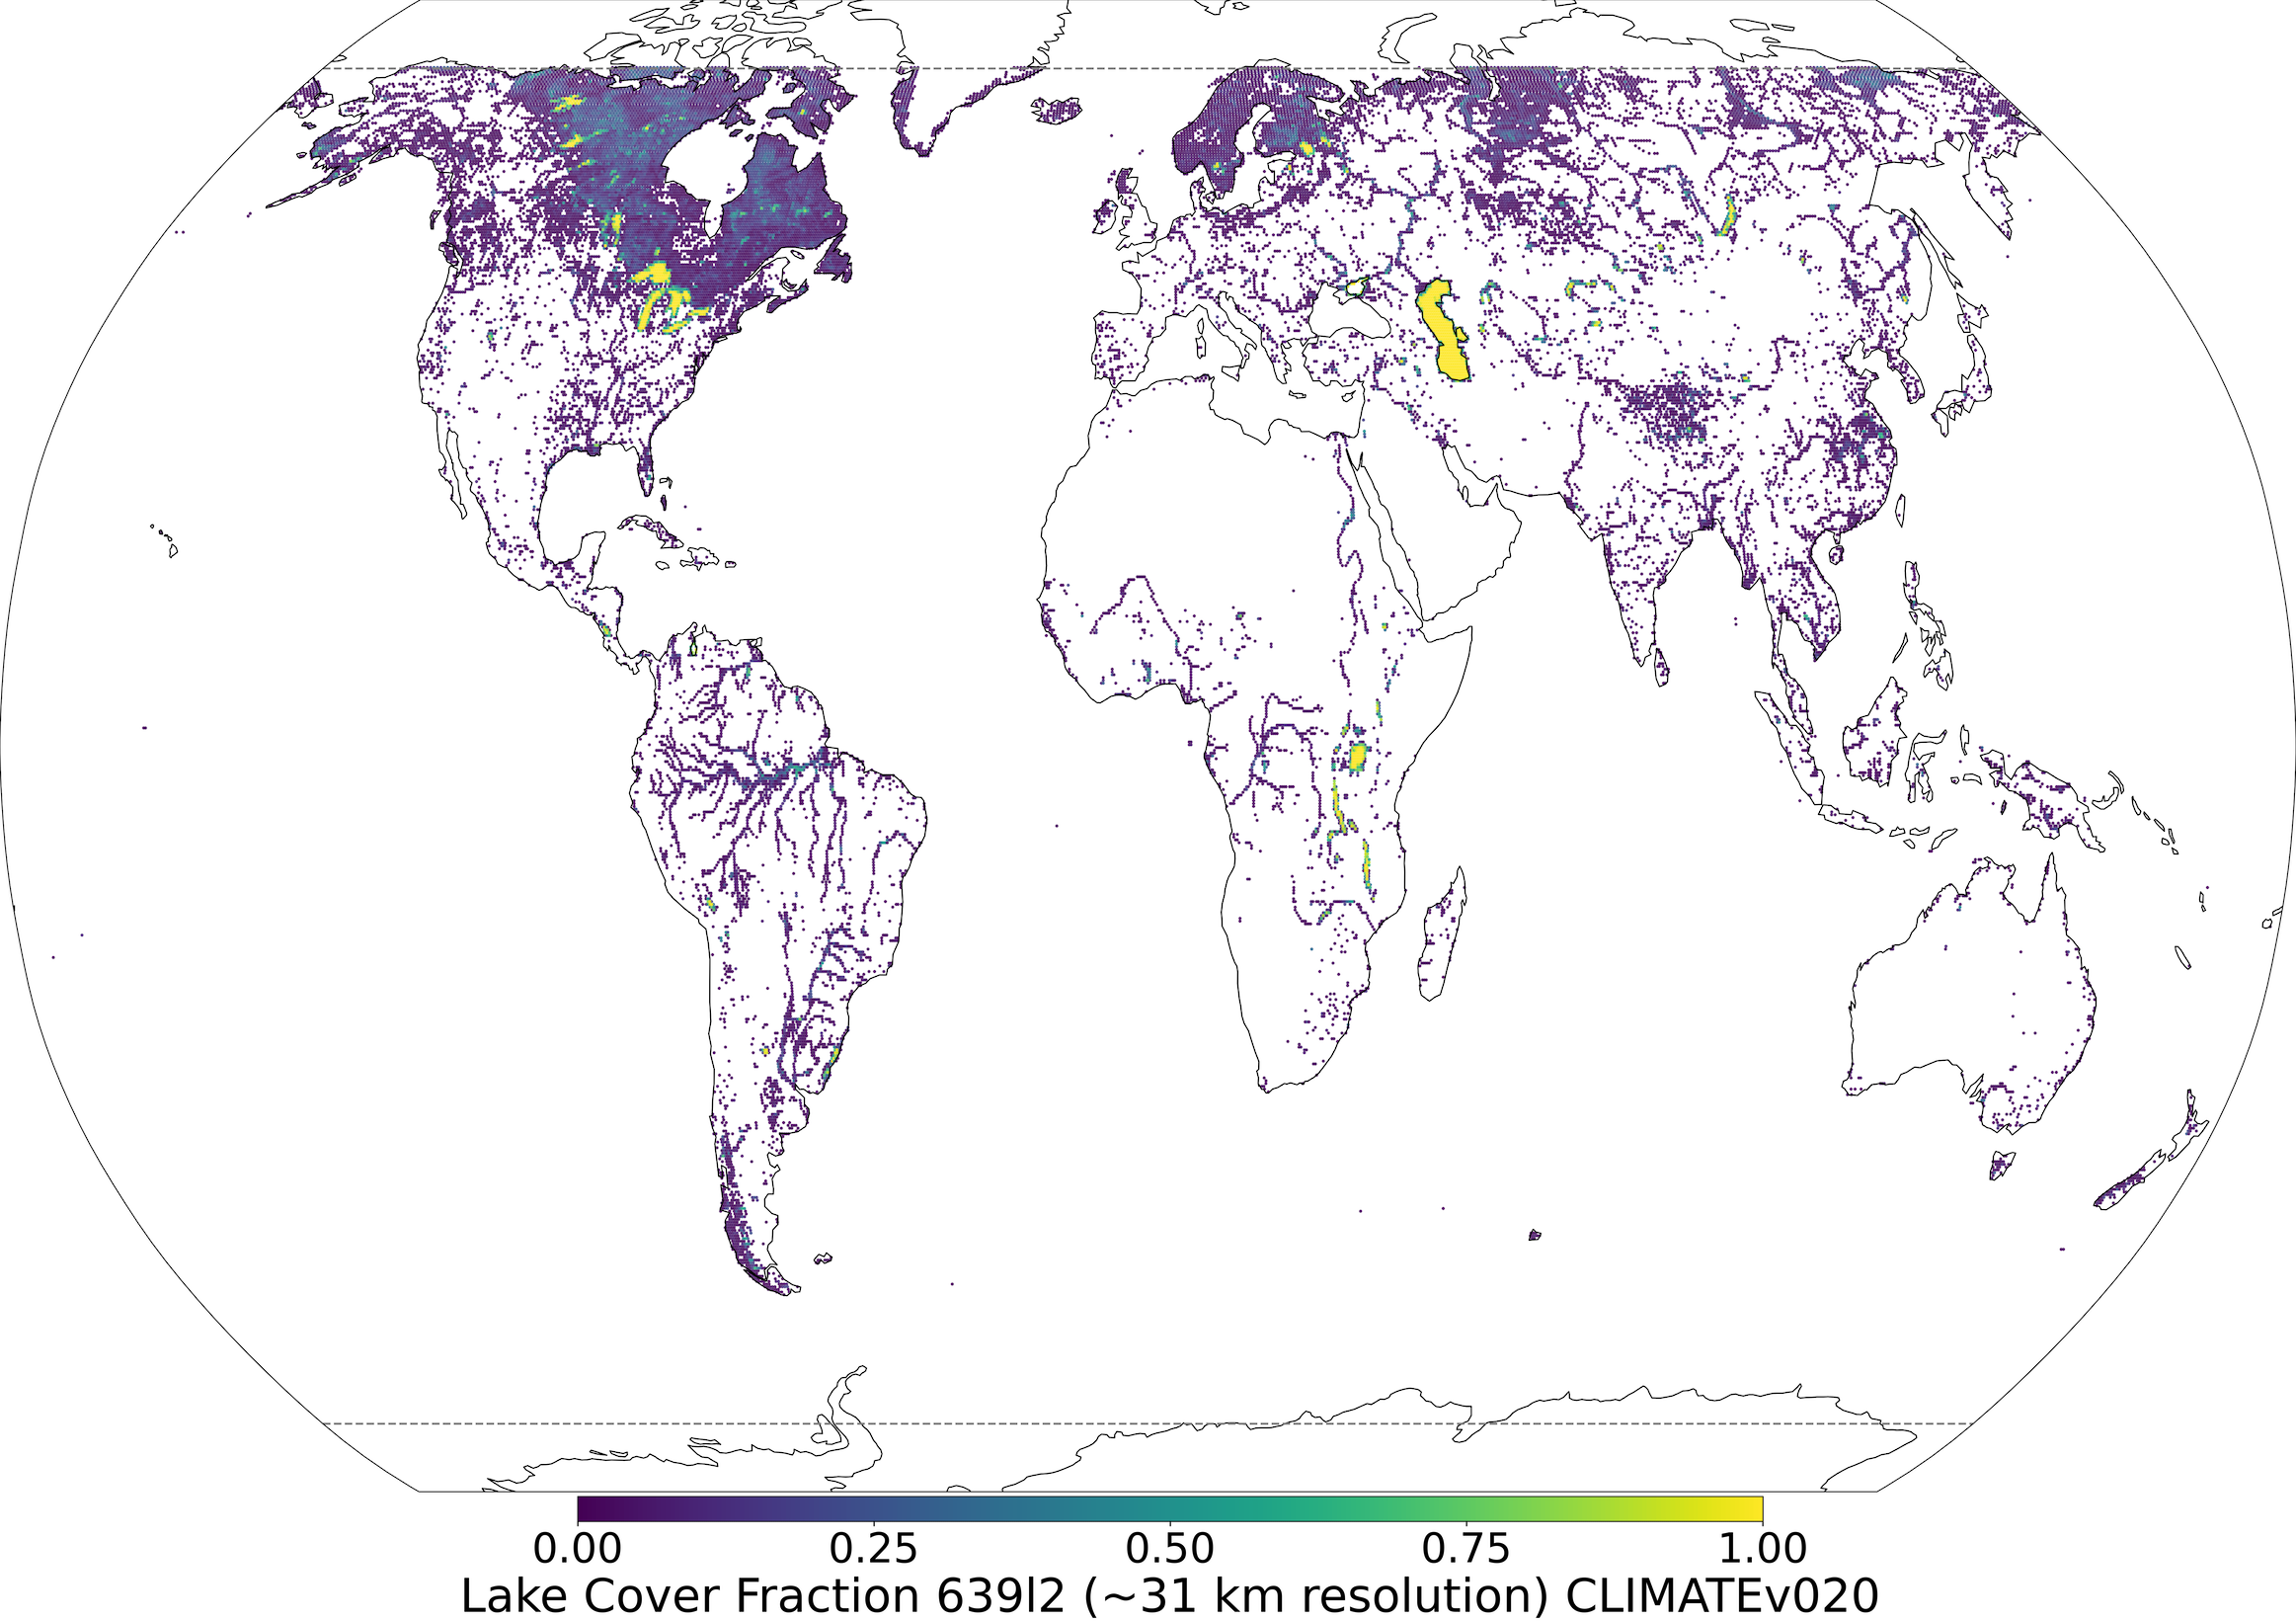
\includegraphics[width=0.48\textwidth]{cl_map}} \\
	\subfloat[\label{fig:cl_delta_map}]{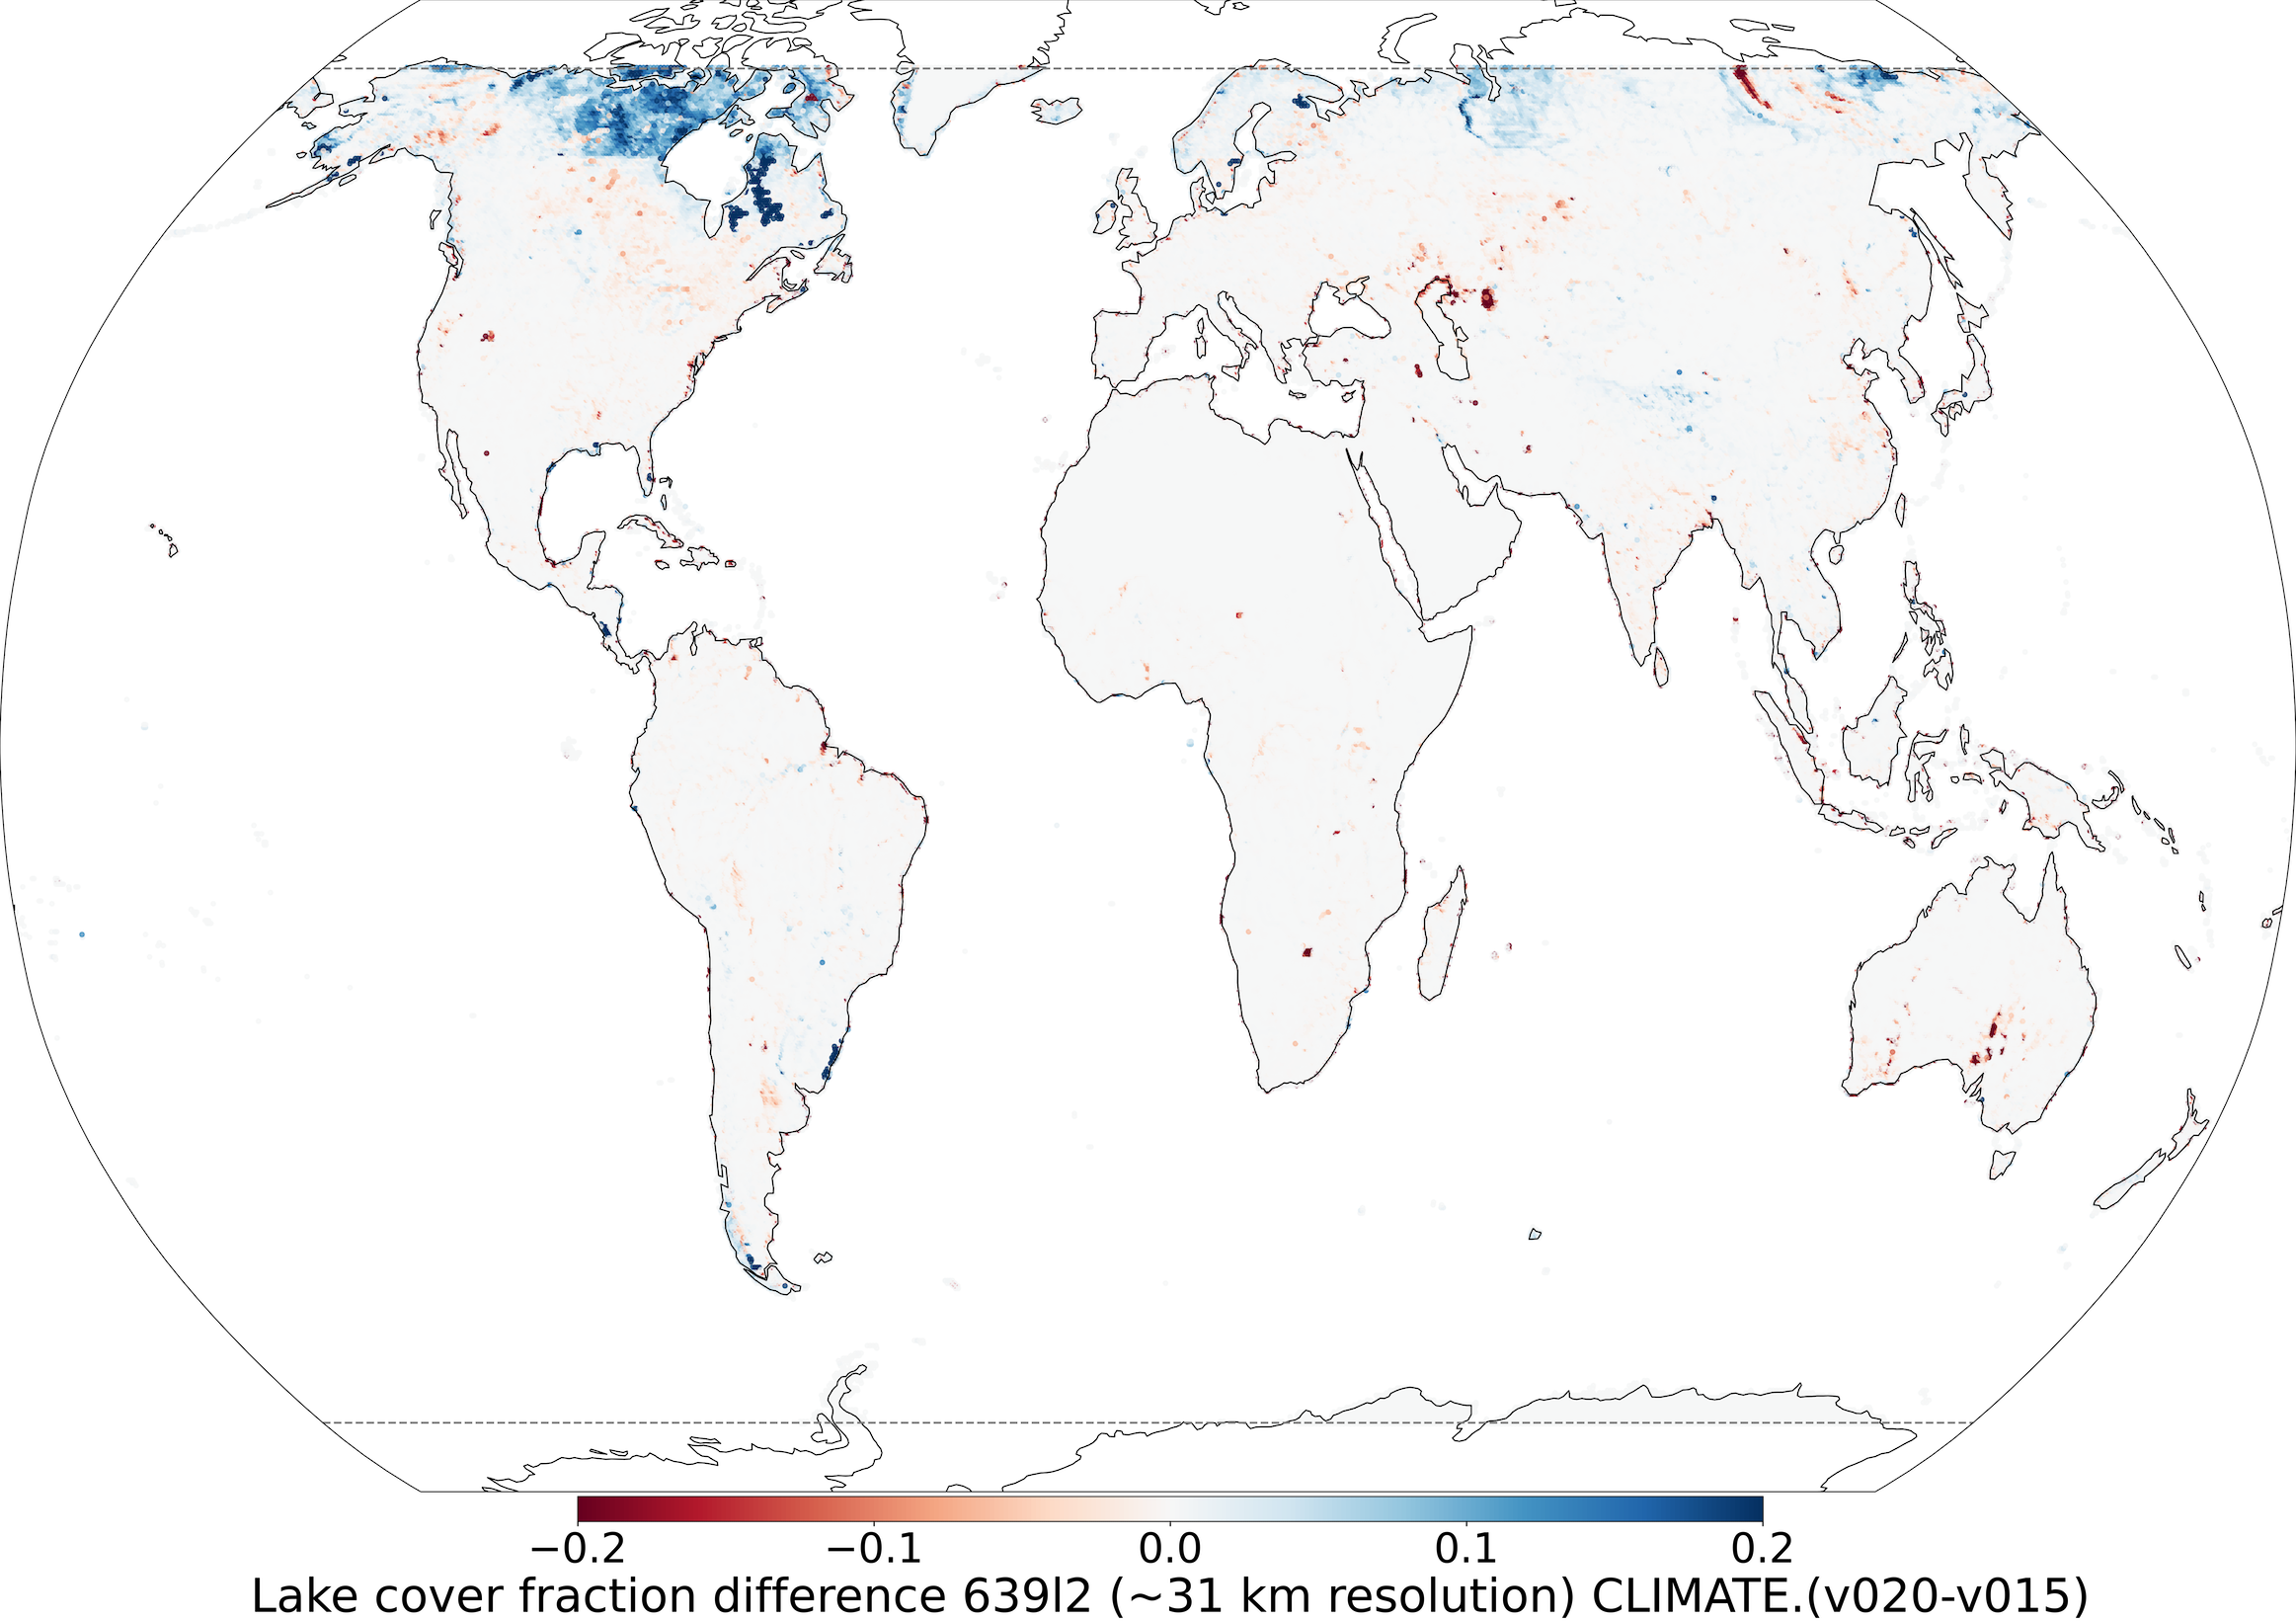
\includegraphics[width=0.48\textwidth]{cl_delta_map}}
	\caption{\DIFaddFL{At $\sim$ 31km resolution (a) V20 fractional lake cover and (b) difference between V20 and V15 lake covers. Over northern latitudes inland water increase in V20 compared to V15 is due to higher resolution input source and its better satellite image recognition methodologies as well as thawing permafrost; inland water reduction in V20 compared to V15 is due to anthropogenic land use changes (e.g. Aral Sea) or due to use of only permanent water (e.g. Australia) which was proven to better represent inland water distribution on annual basis.}} 
	\label{fig:example_figure_a}
\end{figure}



\begin{figure}
	\subfloat[\label{fig:dl_map}]{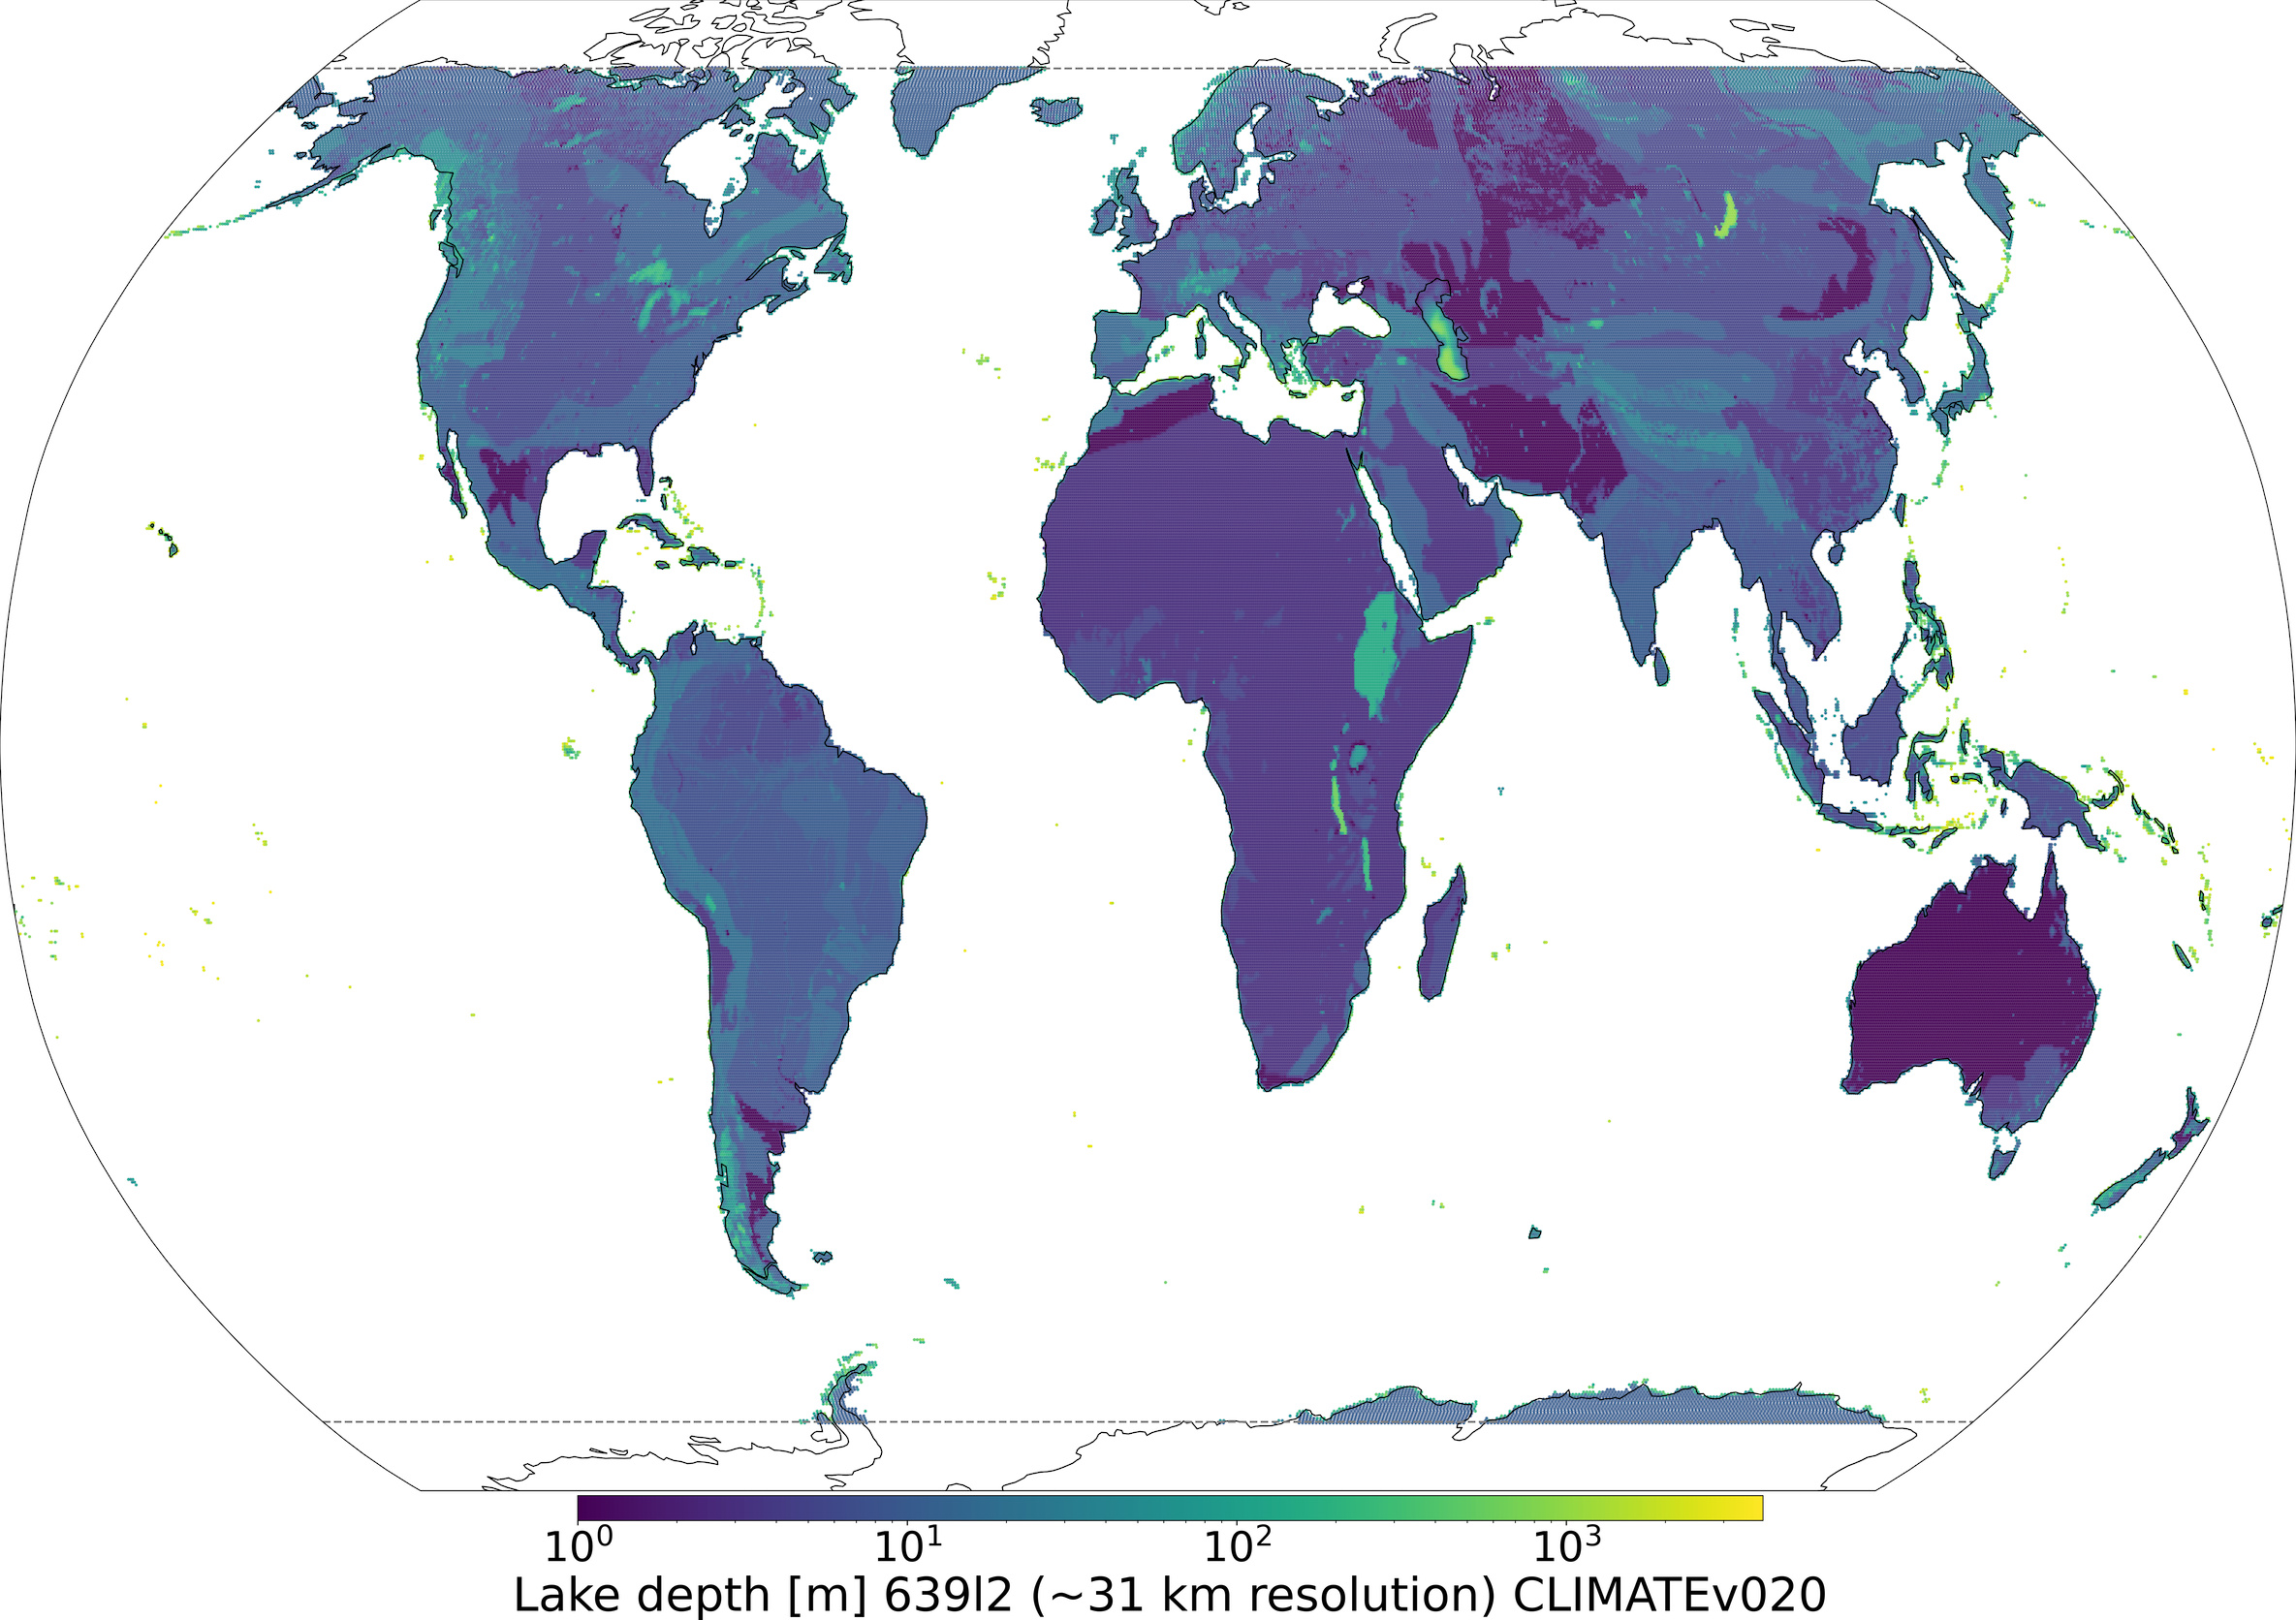
\includegraphics[width=0.48\textwidth]{dl_map}} \\
	\subfloat[\label{fig:dl_delta_map}]{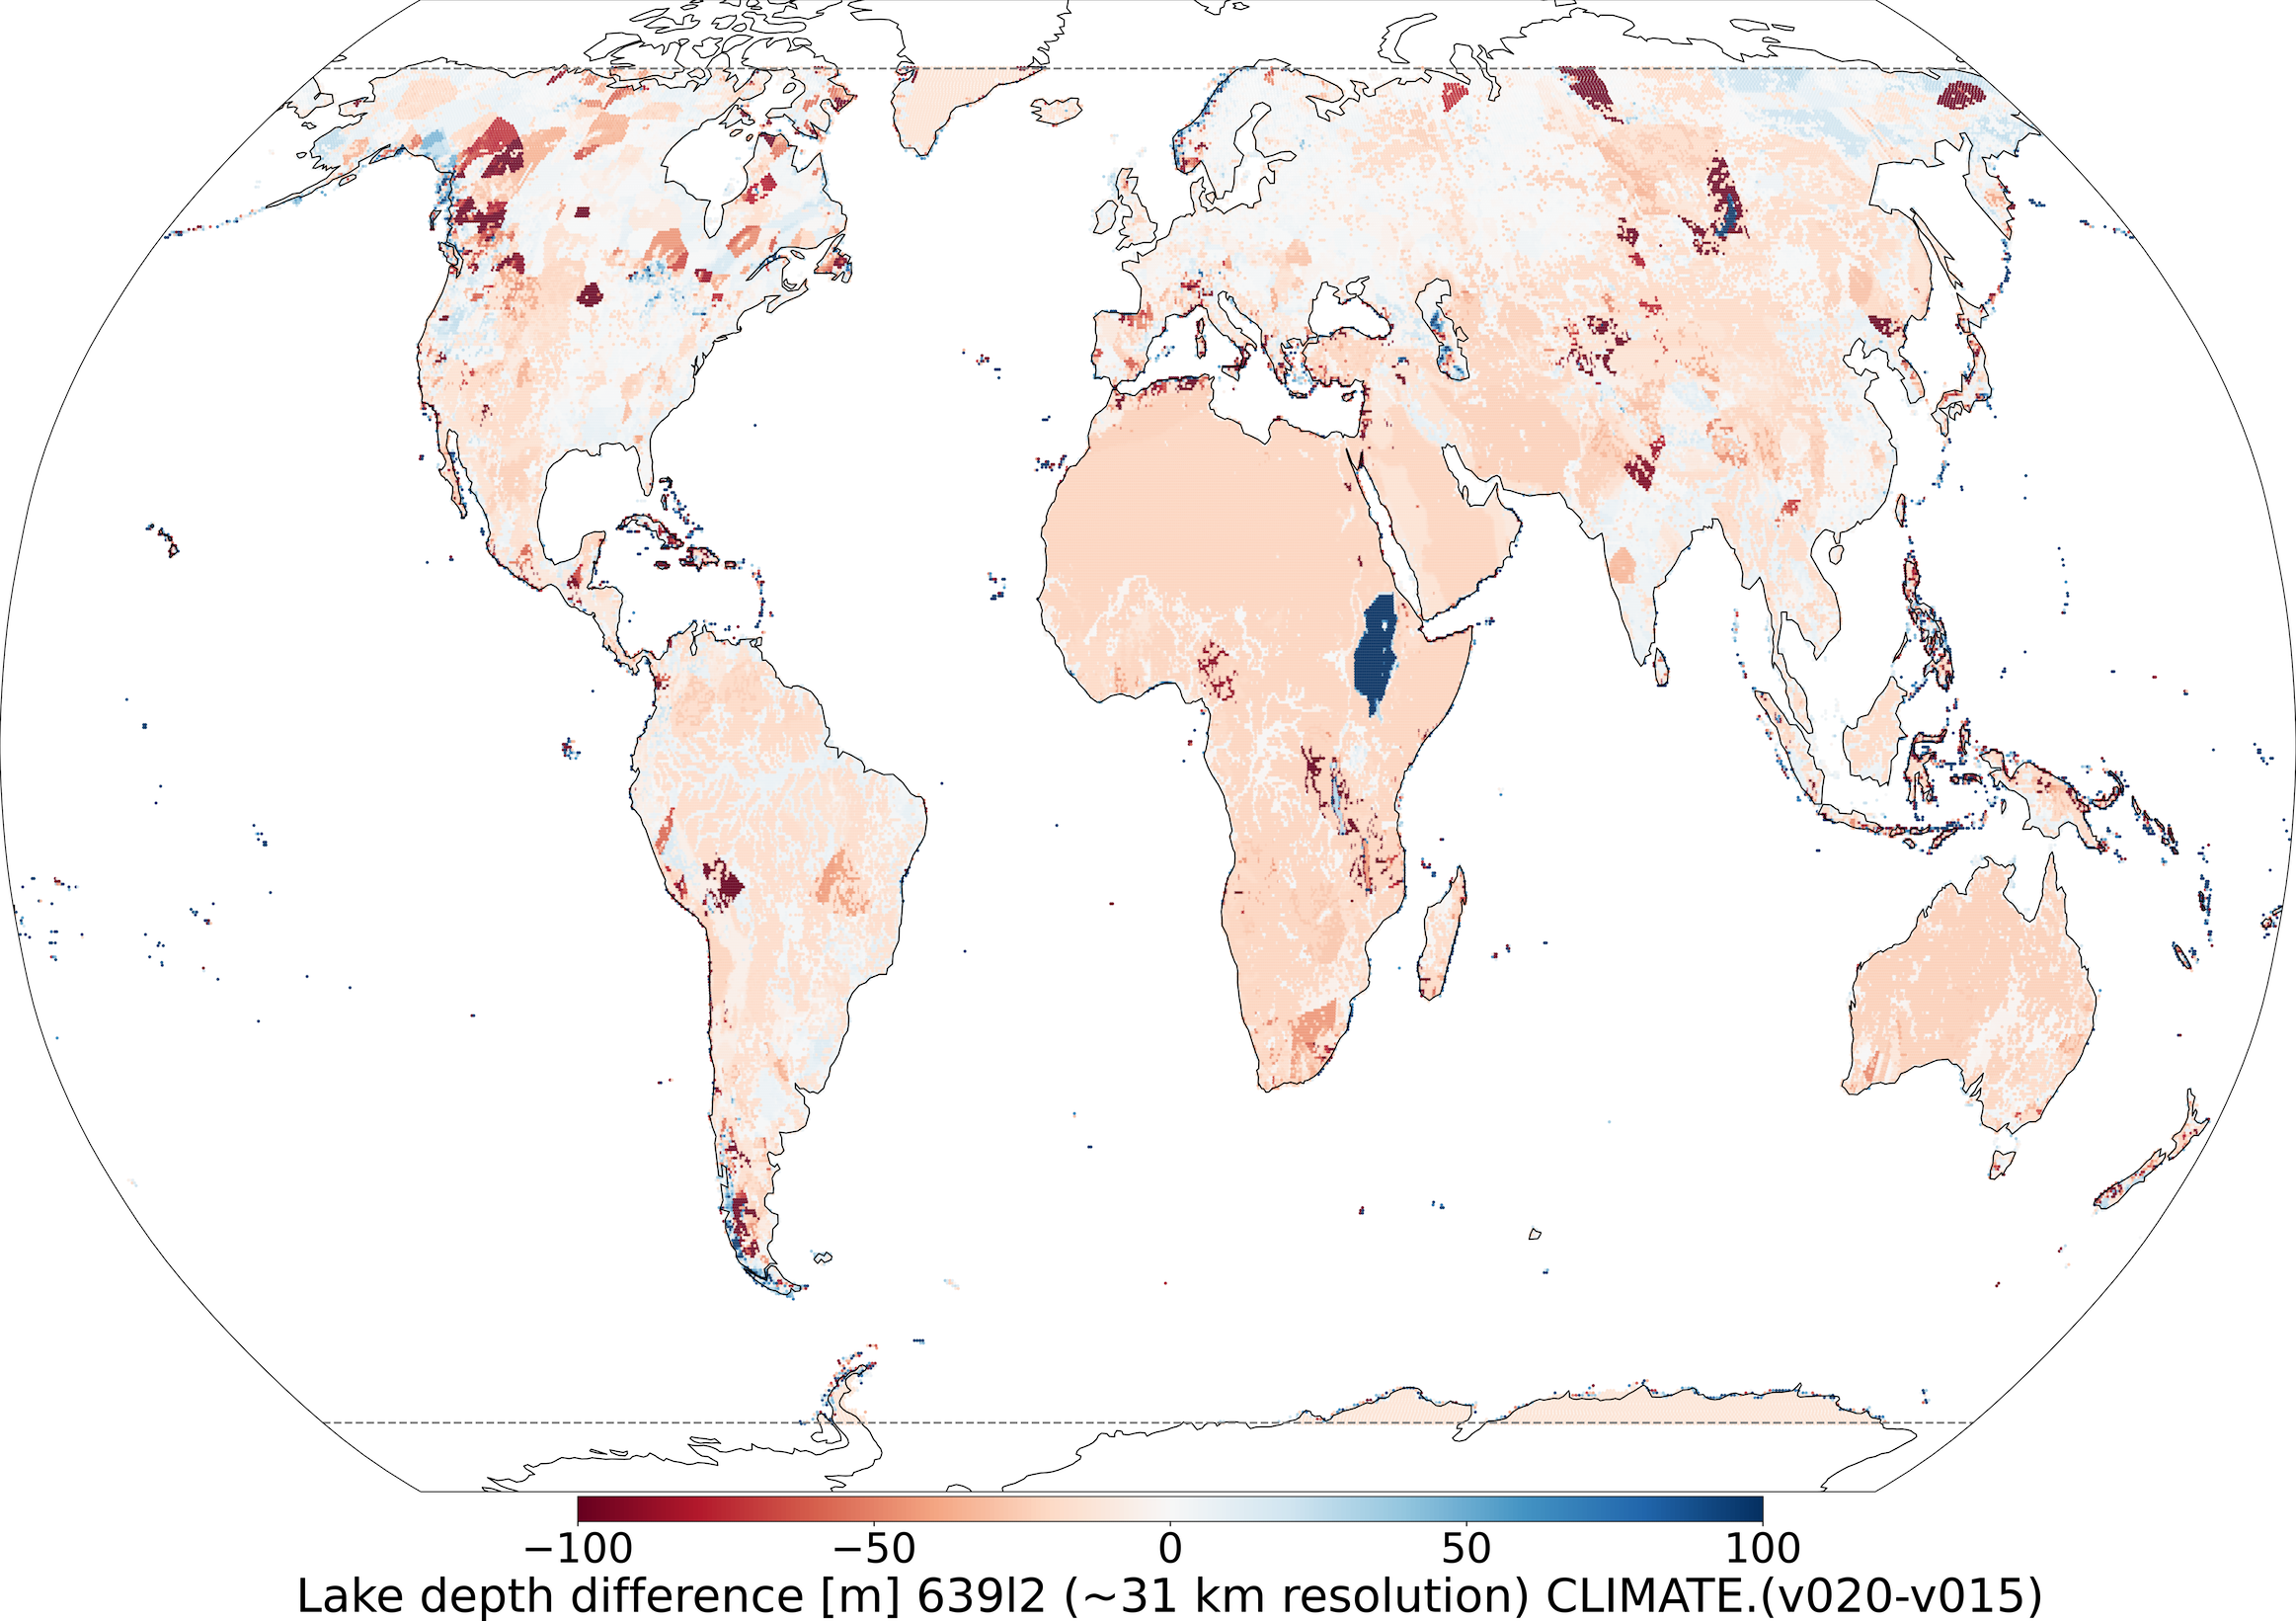
\includegraphics[width=0.48\textwidth]{dl_map_diff}}
	\caption{\DIFaddFL{At $\sim$ 31km resolution (a) V15 lake mean depth in meters and (b) difference between V20 and V15 lake mean depths. In general lake mean depth has decreased in V20 compared to V15 due to the use of mean depth indirect estimates based on geological and climate information, instead of default 25 meter value over lakes without any information.}} 
	\label{fig:example_figure_b}
	\end{figure}




\DIFaddend \subsubsection{ERA5}
\DIFaddbegin \noindent \DIFaddend Climate reanalyses combine observations and modelling to provide calculated values of a range of climactic variables over time. ERA5 is the fifth generation reanalysis from ECMWF. It is produced via 4D-Var data assimilation of the \DIFdelbegin \DIFdel{atmospheric Integrated Forecast system }\DIFdelend \DIFaddbegin \DIFadd{IFS }\DIFaddend cycle 41R2, coupled to a land-surface model \DIFdelbegin \DIFdel{\mbox{%DIFAUXCMD
\cite[ECLand,][]{Boussetta2021} }\hskip0pt%DIFAUXCMD
}\DIFdelend \DIFaddbegin \DIFadd{\mbox{%DIFAUXCMD
\citep[ECLand,][]{Boussetta2021}}\hskip0pt%DIFAUXCMD
, which includes lake parametrization by FLake \mbox{%DIFAUXCMD
\citep{Mironov2008} }\hskip0pt%DIFAUXCMD
}\DIFaddend and an ocean wave model (WAM). The resulting data product provides hourly values of climatic variables across the atmosphere, land and ocean at a resolution of approximately 31km with 137 vertical sigma levels, up to a height of 80km. Additionally, ERA5 provides associated uncertainties of the variables at a reduced 63km resolution via a 10-member Ensemble of Data Assimilations (EDA). \DIFdelbegin \DIFdel{We take }\DIFdelend \DIFaddbegin \DIFadd{In this work }\DIFaddend ERA5 \DIFdelbegin \DIFdel{surface fields on an hourly grain on }\DIFdelend \DIFaddbegin \DIFadd{hourly surface fields at ∼ 31km resolution on }\DIFaddend a reduced Gaussian grid \DIFdelbegin \DIFdel{, with a highest resolution of $\sim$ 31km. Whilst }\DIFdelend \DIFaddbegin \DIFadd{are used. Gaussian grid’s spacing between latitude lines is not regular, but lines are symmetrical along the Equator; the number of points along each latitude line defines longitude lines, which start at longitude 0 and are equally spaced along the latitude line. In a reduced Gaussian grid, the number of points on each latitude line is chosen so that the local east-west grid length remains approximately constant for all latitudes (here Gaussian grid is N320, where N is the number of latitude lines between a Pole and the Equator). The main field used from }\DIFaddend ERA5 \DIFdelbegin \DIFdel{has extensive vertical coverage across 37 pressure levels, for our purposes we will deal solely with surface fields. The }\DIFdelend \DIFaddbegin \DIFadd{is skin temperature (i.e. temperature of the uppermost surface layer, which has no heat capacity and instantaneously responds to changes in surface fluxes) that forms the interface between the soil and the atmosphere. Skin temperature is a theoretical temperature computed by linearizing the surface energy balance equation for each surface type separately, and its feedback on net radiation and ground heat flux is included; for more information see IFS Documentation (2021). ERA5 skin temperature verification against MODIS LST ensemble (i.e. all four MODIS observations were used, namely Aqua Day and Night, Terra Day and Night) over 2003-2018 period showed good correlation between two datasets; errors between ERA5 and MODIS LST ensemble are quite small, i.e. spatially and temporally averaged bias is 1.64 K, root-mean square error (RMSE) is 3.96 K, Pearson correlation coefficient is 0.94, and anomaly correlation coefficient is 0.75 \mbox{%DIFAUXCMD
\citep{essd-13-4349-2021}}\hskip0pt%DIFAUXCMD
. ERA5 skin temperature verification against the Satellite Application Facility on Land Surface Analysis (LSA-SAF) product over Iberian Peninsula showed a general underestimation of daytime LST and slightly overestimation at night-time, relating the large daytime cold bias with vegetation cover differences between ERA5 surface physiography fields and the European Space Agency’s Climate Change Initiative (ESA-CCI) Land Cover dataset; use of ESA-CCI low and high vegetation cover instead of ERA5 ones led to a complete reduction of the large maximum temperature bias during summer \mbox{%DIFAUXCMD
\citep{Johannsen2019}}\hskip0pt%DIFAUXCMD
. ERA5 }\DIFaddend data is obtained via the Copernicus Climate Data Store \DIFdelbegin \DIFdel{\mbox{%DIFAUXCMD
\cite[CDS,][]{CDS}}\hskip0pt%DIFAUXCMD
}\DIFdelend \DIFaddbegin \DIFadd{\mbox{%DIFAUXCMD
\citep[CDS;][]{CDS}}\hskip0pt%DIFAUXCMD
}\DIFaddend .


\subsubsection{Aqua-MODIS}

\DIFdelbegin \DIFdel{Aqua\mbox{%DIFAUXCMD
\cite{aquaref} }\hskip0pt%DIFAUXCMD
}\DIFdelend \DIFaddbegin 


\noindent \DIFadd{Aqua  \mbox{%DIFAUXCMD
\citep{aquaref} }\hskip0pt%DIFAUXCMD
}\DIFaddend is a NASA satellite mission which makes up part of the Earth Observing System (EOS). Operating at an altitude of \DIFdelbegin \DIFdel{700 km}\DIFdelend \DIFaddbegin \DIFadd{700km}\DIFaddend , with orbital period of 99 minutes, its orbital trajectory passes south to north with an equatorial-crossing times in general of \DIFdelbegin \DIFdel{13.30}\DIFdelend \DIFaddbegin \DIFadd{1.30pm}\DIFaddend . This post-meridian crossing time has led to it sometimes being denoted as EOS PM. Launched in 2002 with an initial expected mission duration of 6 years, Aqua has far exceeded its initial brief and \DIFdelbegin \DIFdel{continues to transmit }\DIFdelend \DIFaddbegin \DIFadd{until recently has been transmitting }\DIFaddend information from 4 of the 6 observation instruments on board. \DIFdelbegin \DIFdel{In this work we will concern ourselves with only one of these instruments: MODIS }\DIFdelend \DIFaddbegin \DIFadd{Here we use information only from MODIS instrument}\DIFaddend . MODIS can take surface temperature measurements at a spatial resolution of 1km \DIFaddbegin \DIFadd{(the exact grid size is 0.928km by 0.928km)}\DIFaddend , operating in the wavelength ranges of between \DIFdelbegin \DIFdel{$\sim 3.7 - 4.5 \mu m$ and $\sim 10.9 - 12.3 \mu m$}\DIFdelend \DIFaddbegin \DIFadd{∼3.7-4.5µm and ∼10.9-12.3µm}\DIFaddend . In addition to surface temperature measurements \DIFaddbegin \DIFadd{that were used in this work}\DIFaddend , MODIS can take observations of cloud properties, water vapour, ozone\DIFdelbegin \DIFdel{etc., however for this work we will focus exclusively on the surface temperature measurements. We take }\DIFdelend \DIFaddbegin \DIFadd{, etc. Here }\DIFaddend MYD11A1 v006 \DIFdelbegin \DIFdel{\mbox{%DIFAUXCMD
\cite{MYD11A1} }\hskip0pt%DIFAUXCMD
as our MODIS data product throughout this work which provides daily Land Surface Temperature (LST ) }\DIFdelend \DIFaddbegin \DIFadd{\mbox{%DIFAUXCMD
\citep{MODISusersguide} }\hskip0pt%DIFAUXCMD
collection that provides daily LST }\DIFaddend measurements at a spatial resolution of 1km on a sinusoidal projection grid SR-ORG:6974 \DIFdelbegin \DIFdel{, which }\DIFdelend \DIFaddbegin \DIFadd{(}\DIFaddend takes a spherical projection \DIFdelbegin \DIFdel{ellipsoid }\DIFdelend but a WGS84 datum ellipsoid\DIFdelbegin \DIFdel{. For our purposes, daily information over several years is needed, so to }\DIFdelend \DIFaddbegin \DIFadd{) is exercised. Daily global LST data is generated by first applying a split-window LST algorithm \mbox{%DIFAUXCMD
\citep{508406} }\hskip0pt%DIFAUXCMD
on all nominal (i.e. 1km at nadir) resolution swath (scene) with a nominal coverage of ~5 minutes of MODIS scans along the track acquired in daytime, and secondly by mapping results onto integerized sinusoidal projection; for more details see \mbox{%DIFAUXCMD
\cite{MODISusersguide} }\hskip0pt%DIFAUXCMD
and Figure \ref{fig:example_figure_c}. Validation of this product was carried out using temperature-based method over different land cover types (e.g. grasslands, croplands, shrublands, woody areas, etc.) in several regions around the globe (i.e. United States, Portugal, Namibia, and China) at different atmospheric and/or surface conditions; the best accuracy is achieved over United States sites with RMSE lower than 1.3K \mbox{%DIFAUXCMD
\citep{DUAN201916}}\hskip0pt%DIFAUXCMD
. At large view angles and in semi-arid regions the data product may have slightly higher errors due to rather uncertain classification-based surface emissivities and heavy dust aerosols effects. In addition, the MODIS cloud mask struggles to eliminate all cloud and/or heavy aerosols contaminated grid-cells from the clear-sky ones (LST errors in such grid-cells can be 4-11K and larger). Validation of this product over five bare ground sites in north Africa (in total 12 radiosonde-based datasets validated) showed that mean LST error was within $\pm$0.6K (with exception for one dataset, where mean LST error was 0.8K) and standard deviation of LST errors were less than 0.5K \mbox{%DIFAUXCMD
\citep{DUAN201916}}\hskip0pt%DIFAUXCMD
. In this work to }\DIFaddend reduce the amount of \DIFdelbegin \DIFdel{data }\DIFdelend \DIFaddbegin \DIFadd{daily data over multiple years }\DIFaddend to store and manipulate, \DIFdelbegin \DIFdel{this data product is then }\DIFdelend \DIFaddbegin \DIFadd{prior use LST data is (i) }\DIFaddend filtered to contain only cloud free data\DIFdelbegin \DIFdel{and }\DIFdelend \DIFaddbegin \DIFadd{, and (ii) }\DIFaddend averaged to a \DIFdelbegin \DIFdel{4 km }\DIFdelend \DIFaddbegin \DIFadd{~4km at the Equator }\DIFaddend resolution on a regular latitude-longitude grid, EPSG\DIFdelbegin \DIFdel{4326. Only }\DIFdelend \DIFaddbegin \DIFadd{:4326 (note that only }\DIFaddend grid cells which have 8 or more valid observations at 1km resolution are averaged over, otherwise they are classified as missing data\DIFaddbegin \DIFadd{)}\DIFaddend .

%DIF < 
%DIF < https://spatialreference.org/ref/sr-org/modis-sinusoidal-3/
\DIFaddbegin \begin{figure}
	\subfloat[\label{fiig:Modistime1}]{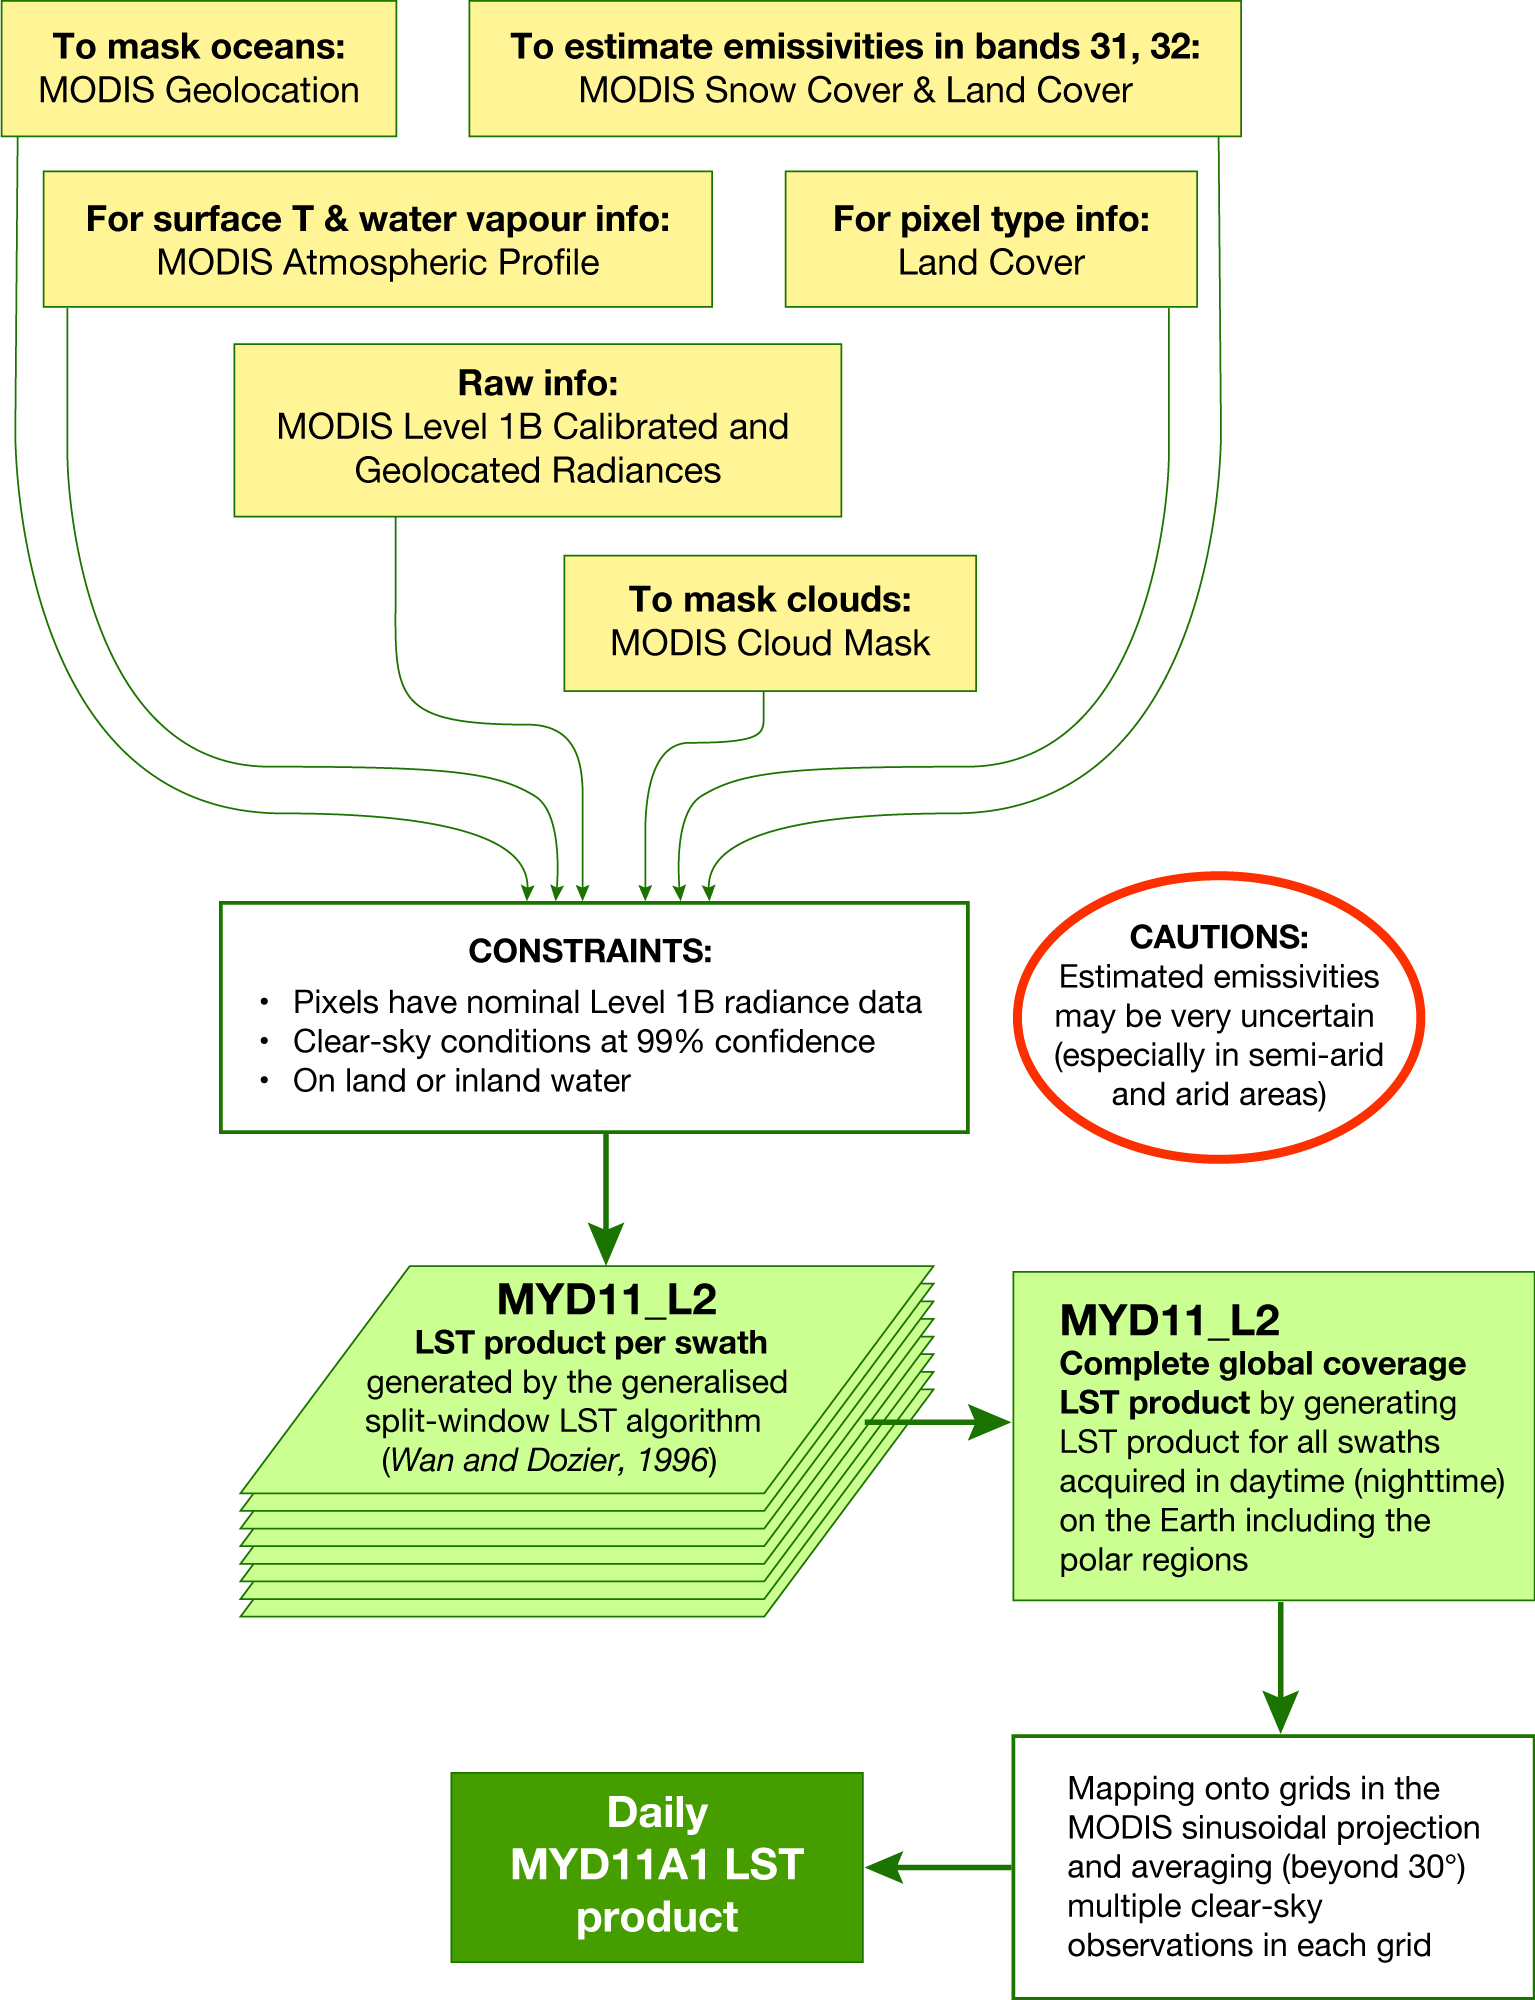
\includegraphics[width=0.48\textwidth]{MODIS_flow}} \\
	\caption{\DIFaddFL{A brief step-by-step explanation of the LST algorithm for MYD11A1 v006 collection.}} 
	\label{fig:example_figure_c}
\end{figure}

\DIFaddend 

\subsection{Joining the data}\label{sec:join}
\DIFdelbegin \DIFdel{For a given hour in time we have a selection of }\DIFdelend \DIFaddbegin \DIFadd{To join selected }\DIFaddend ERA5 \DIFdelbegin \DIFdel{data that covers the entire globe at a ``low" (31 km) resolution }\DIFdelend \DIFaddbegin \DIFadd{global fields }\DIFaddend on a reduced Gaussian grid \DIFdelbegin \DIFdel{and a strip of MODIS data at ``high" (4km) resolution }\DIFdelend \DIFaddbegin \DIFadd{at $\sim$ 31km resolution (information in UTC, 24 hourly maps per day) with Aqua-MODIS global LST data }\DIFaddend on a regular \DIFdelbegin \DIFdel{grid. We want to be able to join these two datasets in both space and time. That is to say, given a location on the Earth's surface at a particular point in time, what is the observed MODIS LST and the values of corresponding ERA fields? This step is key if we then want to train a model to learn the mapping between ERA5 and MODIS. }%DIFDELCMD < \newline 
%DIFDELCMD < 

%DIFDELCMD < \noindent %%%
\DIFdel{In order to proceed it is first }\DIFdelend \DIFaddbegin \DIFadd{latitude-longitude grid at ~4km resolution (information in local solar time, 1 map per day), both datasets need to be at the same time space. First it is }\DIFaddend necessary to determine the absolute time (i.e. UTC) at which the MODIS observations were taken. Since \DIFaddbegin \DIFadd{in general }\DIFaddend all Aqua observations are taken at \DIFdelbegin \DIFdel{a }\DIFdelend \DIFaddbegin \DIFadd{1.30pm }\DIFaddend local solar time\DIFdelbegin \DIFdel{of 13.30, we can relate this straightforwardly }\DIFdelend \DIFaddbegin \DIFadd{, it can be related }\DIFaddend to a UTC via \DIFdelbegin \DIFdel{the longitudeof observations as, }\DIFdelend \DIFaddbegin \DIFadd{observation longitude, following Eq. \ref{eq:time_conversion}:
}\DIFaddend \begin{equation}
	\text{UTC} = \text{Local solar time} - \frac{\text{longitude}}{15} \ , 
	\DIFaddbegin \label{eq:time_conversion}
\DIFaddend \end{equation}
where \DIFdelbegin \DIFdel{the }\DIFdelend \DIFaddbegin \DIFadd{longitude is in degrees, and }\DIFaddend UTC is rounded to the nearest hour. \DIFdelbegin \DIFdel{Naturally, this }\DIFdelend \DIFaddbegin \DIFadd{This }\DIFaddend conversion is inexact since there is an additional correction as a function of the latitude, \DIFdelbegin \DIFdel{but we follow }\DIFdelend \DIFaddbegin \DIFadd{yet recommended by }\DIFaddend the official MODIS Products User’s Guide \DIFdelbegin \DIFdel{\mbox{%DIFAUXCMD
\cite{MODISusersguide} }\hskip0pt%DIFAUXCMD
which recommends converting between longitude and UTC in this way}\DIFdelend \DIFaddbegin \DIFadd{\mbox{%DIFAUXCMD
\citep{MODISusersguide}}\hskip0pt%DIFAUXCMD
}\DIFaddend ; given the short orbital period of Aqua these \DIFaddbegin \DIFadd{additional }\DIFaddend higher order corrections are expected to be typically small \DIFdelbegin \DIFdel{. We have also confirmed the accuracy of this }\DIFdelend \DIFaddbegin \DIFadd{and for our purposes can be neglected. Also, the }\DIFaddend assumption that all Aqua observations are taken at \DIFdelbegin \DIFdel{a }\DIFdelend \DIFaddbegin \DIFadd{1.30pm }\DIFaddend local solar time \DIFdelbegin \DIFdel{of 13.30 (see Fig. \ref{fig:MODIS_time}}\DIFdelend \DIFaddbegin \DIFadd{was checked (see Figure \ref{fig:MODIS_time_error}}\DIFaddend ). The annually averaged mean \DIFdelbegin \DIFdel{difference }\DIFdelend \DIFaddbegin \DIFadd{time difference at ~31km resolution (i.e. daily differences between local solar time of observations and 1.30pm at 1km resolution were first aggregated to 31km resolution using averaging, and then aggregated in time over a year) }\DIFaddend is 0.16 \DIFdelbegin \DIFdel{or ~}\DIFdelend \DIFaddbegin \DIFadd{hours or }\DIFaddend 10 \DIFdelbegin \DIFdel{min (MAEis }\DIFdelend \DIFaddbegin \DIFadd{minutes, with mean absolute error (MAE) being }\DIFaddend 0.46 \DIFdelbegin \DIFdel{or ~}\DIFdelend \DIFaddbegin \DIFadd{hours or }\DIFaddend 28 \DIFdelbegin \DIFdel{min, RMSE is }\DIFdelend \DIFaddbegin \DIFadd{minutes and RMSE being }\DIFaddend 0.61 \DIFdelbegin \DIFdel{or ~}\DIFdelend \DIFaddbegin \DIFadd{hours or }\DIFaddend 37 \DIFdelbegin \DIFdel{min}\DIFdelend \DIFaddbegin \DIFadd{minutes (current values correspond 70N-70S region year 2019, but confirmed to be approximately identical for each year of 2016-2019 period}\DIFaddend ). Since the \DIFdelbegin \DIFdel{ERA5 data has a }\DIFdelend temporal resolution of \DIFdelbegin \DIFdel{an hour, this level of accuracy is sufficient. The conversion generally }\DIFdelend \DIFaddbegin \DIFadd{ERA5 data is hourly, the assumptions inherent to Eq \ref{eq:time_conversion} are sufficiently accurate. Over the poles (i.e. 90-70°N and 70-90°S) satellite sweeps overlap significantly and in general conversion }\DIFaddend becomes less accurate \DIFdelbegin \DIFdel{as one moves towards the poles; on a daily timescale differences at the poles }\DIFdelend \DIFaddbegin \DIFadd{(daily time differences }\DIFaddend can reach more than \DIFdelbegin \DIFdel{±}\DIFdelend \DIFaddbegin \DIFadd{$\pm$ }\DIFaddend 3.5 hours\DIFdelbegin \DIFdel{, for this reason we restrict our analysisthroughout this work to grid points with $|\theta| < 70^{\circ}$}\DIFdelend \DIFaddbegin \DIFadd{), so these areas were not included in the analysis}\DIFaddend . \newline 

\DIFdelbegin %DIFDELCMD < \begin{figure}
%DIFDELCMD < 	\subfloat[\label{fiig:Modistime1}]{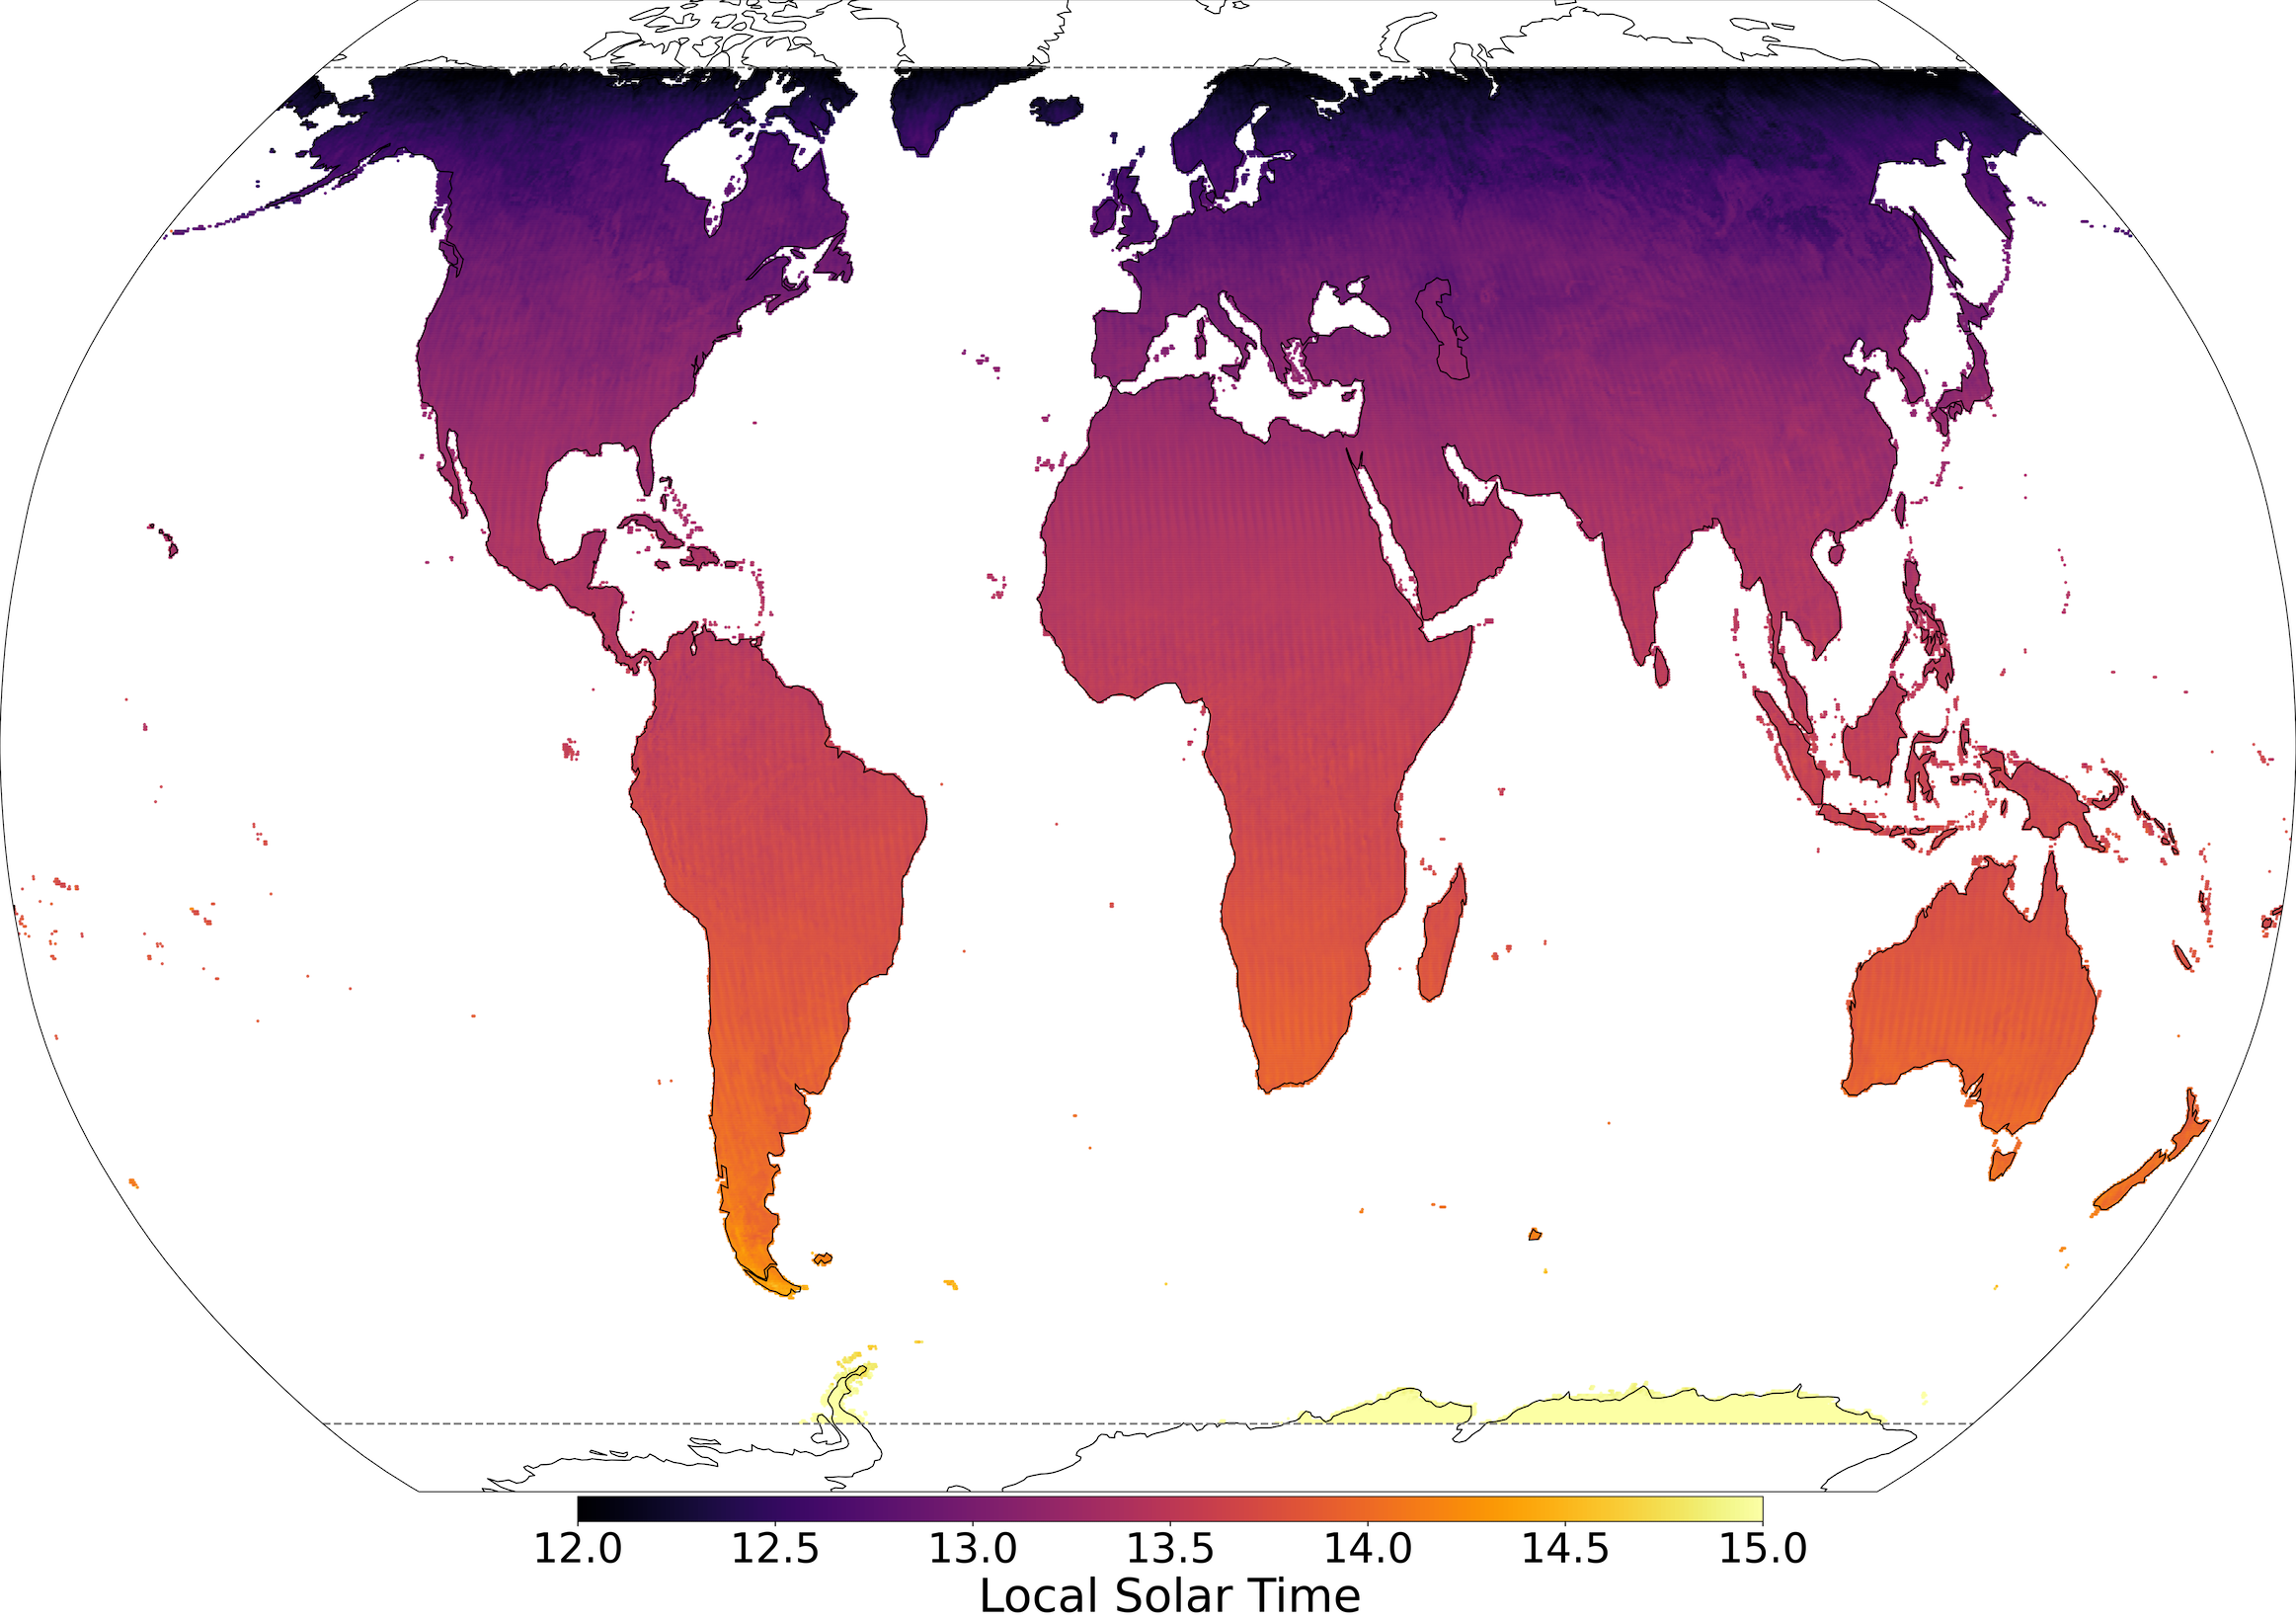
\includegraphics[width=0.48\textwidth]{MODIS_local_solar_time}} \\
%DIFDELCMD < 	\subfloat[\label{fig:Modistime1}]{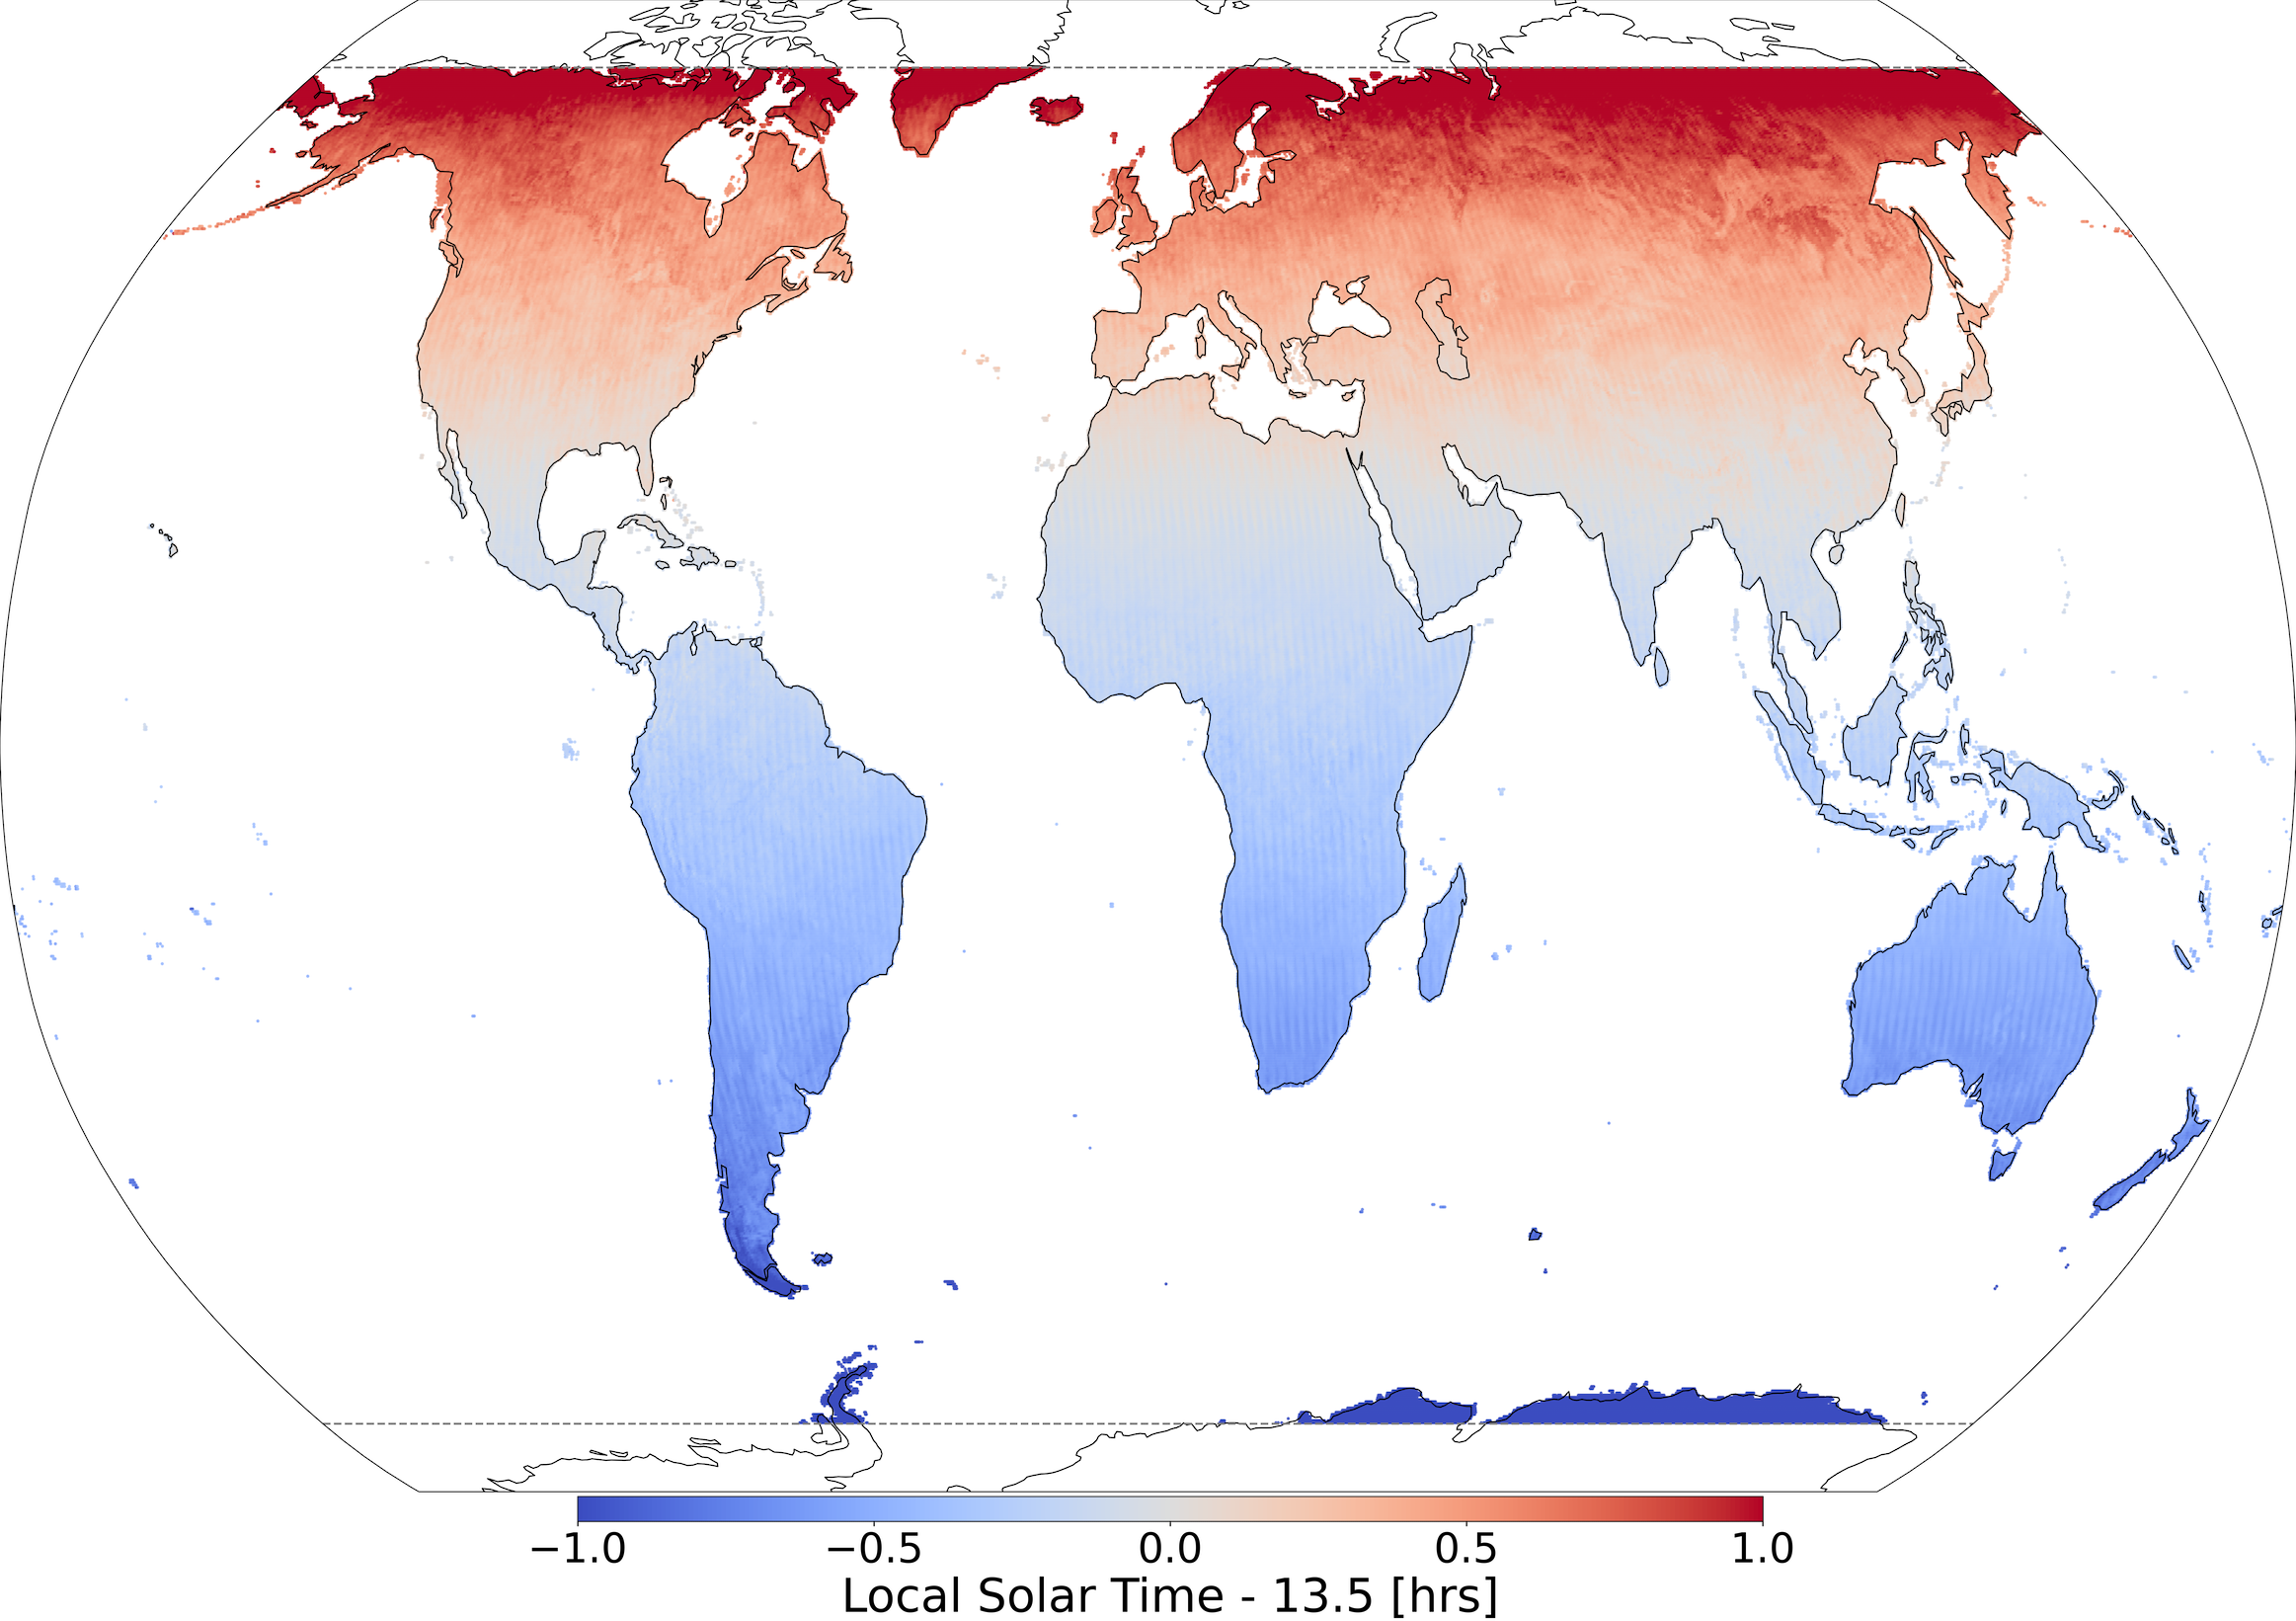
\includegraphics[width=0.48\textwidth]{MODIS_local_solar_time_diff}}
%DIFDELCMD < 	%%%
%DIFDELCMD < \caption{%
{%DIFAUXCMD
\DIFdelFL{Average }\textit{\DIFdelFL{(a)}} %DIFAUXCMD
\DIFdelFL{Local solar time of MODIS Aqua day, }\textit{\DIFdelFL{(b)}} %DIFAUXCMD
\DIFdelFL{Error relative to the assumed local solar time of 13.30 for the year 2019 at a 31km resolution. The errors are generally sub-hr and grow at greater latitudes. We exclude data with latitudes $|\theta| < 70^{\circ}$ and take 13.30 as a constant local solar time.}} 
	%DIFAUXCMD
%DIFDELCMD < \label{fig:MODIS_time}
%DIFDELCMD < \end{figure}
%DIFDELCMD < %%%
\DIFdelend 

\DIFdelbegin %DIFDELCMD < \begin{figure}
%DIFDELCMD < 	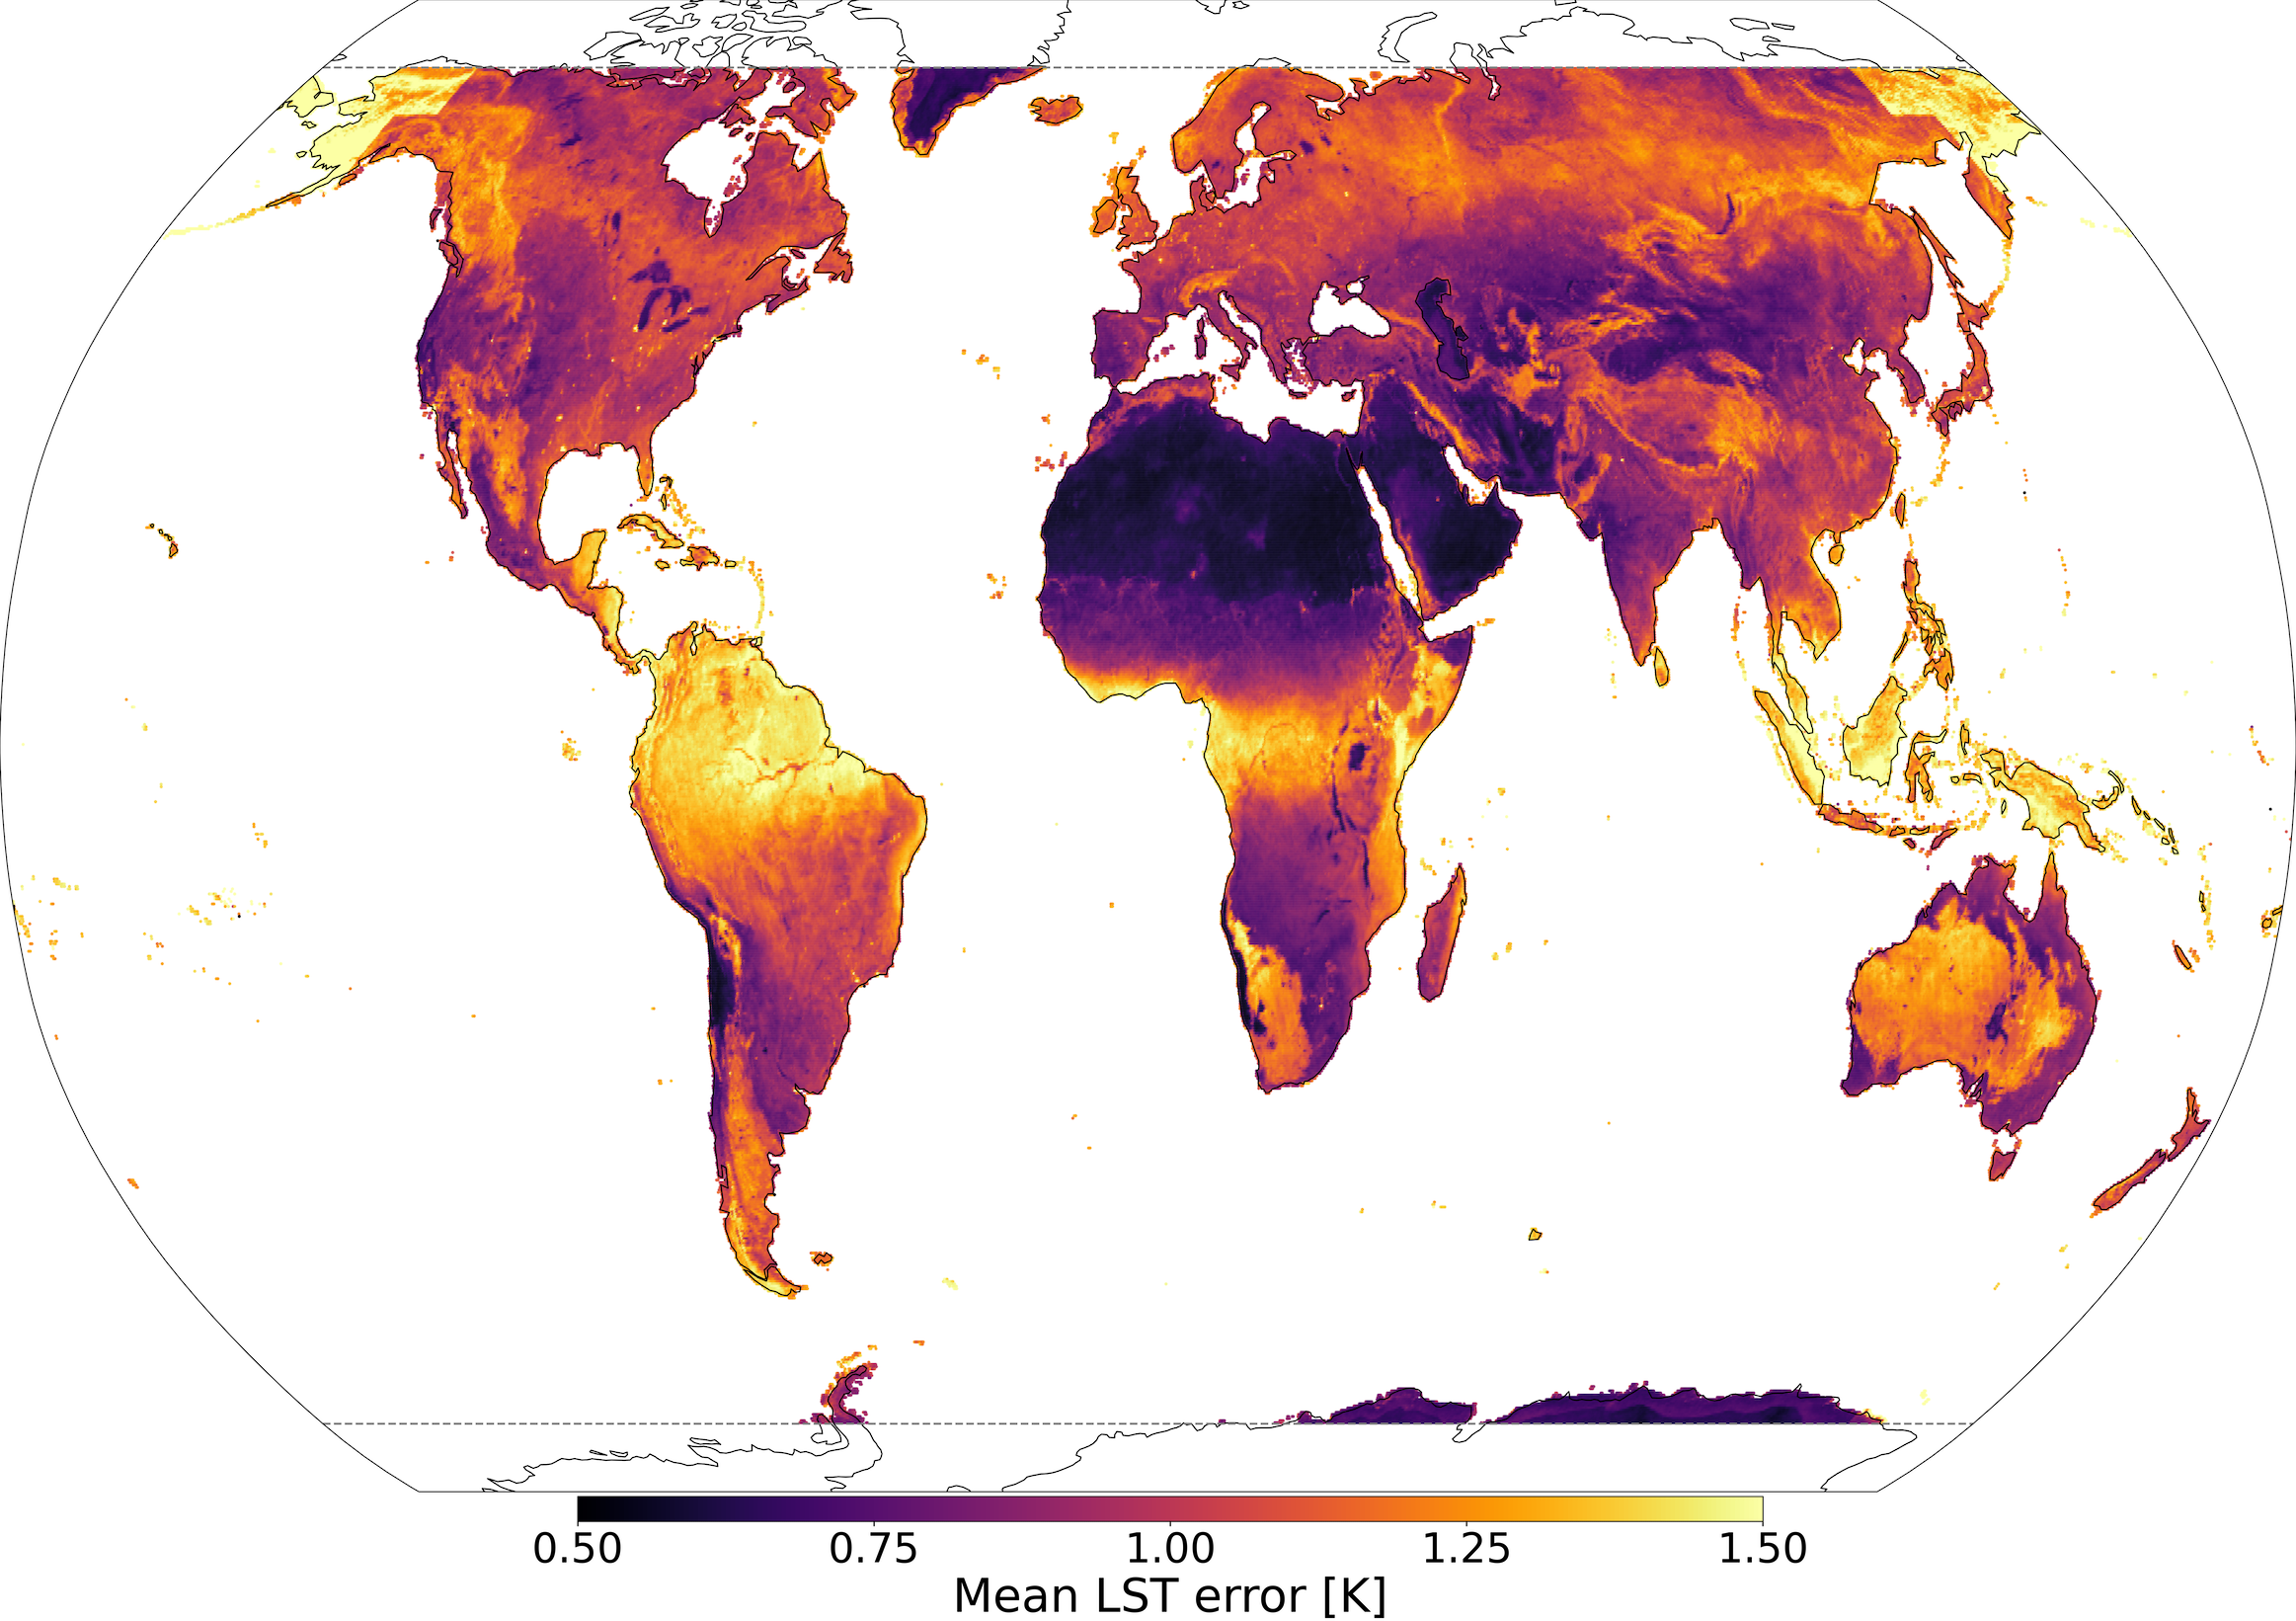
\includegraphics[width=0.48\textwidth]{MODIS_obs_error}
%DIFDELCMD < 	%%%
%DIFDELCMD < \caption{%
{%DIFAUXCMD
\DIFdelFL{Average error in the MODIS LST measurement at a 31km resolution. The raw MODIS data at a 1km resolution provides categorical LST errors with bins $\leq 1$K, $1 - 2$K $2-3$K and $>3$K. When averaging to 31km resolution we compute a weighted average over the 1km grid cells, where we take the median bin value, and $5$K for the $>3$K bin.}} 
	%DIFAUXCMD
%DIFDELCMD < \label{fig:MODIS_obs_error}
%DIFDELCMD < \end{figure}
%DIFDELCMD < 

%DIFDELCMD < %%%
\DIFdelend \noindent \DIFdelbegin \DIFdel{With the MODIS data converted to an hourly UTCit is then straightforward to match this to the corresponding hour in the ERA dataset. In order to then match in space we select an hour of data and do the following }\DIFdelend \DIFaddbegin \DIFadd{Once Aqua-MODIS time of observation is converted to UTC, Aqua-MODIS data at $\sim$ 4km resolution is matched in time and space to ERA5 information in a following way}\DIFaddend :
\begin{enumerate}
	\item Take a single \DIFdelbegin \DIFdel{MODIS }\DIFdelend \DIFaddbegin \DIFadd{Aqua-MODIS }\DIFaddend LST observation at a particular point on the MODIS grid\DIFdelbegin \DIFdel{.
	}\DIFdelend \DIFaddbegin \DIFadd{;
	}\DIFaddend \item \DIFaddbegin \DIFadd{Select ERA5 global hourly map matching Aqua-MODIS LST observation time in UTC;
	}\item \DIFaddend Find the nearest point on the ERA5 grid to that MODIS grid point\DIFdelbegin \DIFdel{.
	}\DIFdelend \DIFaddbegin \DIFadd{;
	}\DIFaddend \item Repeat \DIFdelbegin \DIFdel{for every MODIS observation}\DIFdelend \DIFaddbegin \DIFadd{previous steps for every Aqua-MODIS observation;
	}\DIFaddend \item Group \DIFaddbegin \DIFadd{matched data pairs }\DIFaddend by the ERA5 grid points, averaging over all the \DIFdelbegin \DIFdel{MODIS }\DIFdelend \DIFaddbegin \DIFadd{Aqua-MODIS }\DIFaddend observations that are associated with each ERA5 point.
\end{enumerate}
\DIFdelbegin \DIFdel{The result }\DIFdelend \DIFaddbegin \DIFadd{At the end }\DIFaddend of this process \DIFdelbegin \DIFdel{is then for every set of }\DIFdelend \DIFaddbegin \DIFadd{selected }\DIFaddend ERA5 \DIFdelbegin \DIFdel{input fields at a particular point in space and time , we have an empirical LST ``observation " which is an average over $n$ MODIS observations (see e. g. Fig \ref{fig:MODIS_obs}) . We take this averaged observation as the ground truth }\DIFdelend \DIFaddbegin \DIFadd{fields are mapped to a single Aqua-MODIS time of observation and Aqua-MODIS LST data is mapped (i.e. multiple Aqua-MODIS observations could be averaged over, see Figure \ref{fig:modis_plot_1}) to a reduced Gaussian grid at ~31km resolution; averaged Aqua-MODIS observations are considered as ground truth (i.e. targets }\DIFaddend $y$\DIFdelbegin \DIFdel{that we are }\DIFdelend \DIFaddbegin \DIFadd{) that VESPER is }\DIFaddend trying to predict\DIFaddbegin \DIFadd{. To better understand VESPER’s grid-cell results at ~31km resolution additional information was computed from Aqua-MODIS, namely (i) total number of valid observations per month and year (see Figure \ref{fig:modis_plot_1}), and (ii) average LST error based on Aqua-MODIA quality assessment (i.e. quality flag, see Figure \ref{fig:modis_plot_2}). Based on this additional information it can be concluded that areas with sparse number of observations in general have more uncertain LST values; exceptions are Alaska in United States and Anadyrsky District in Russia (area 30° east and west from 180°E around 70-60°N), deserts of Australia and Kalahari desert in Namibia, Botswana and South Africa, where majority of vast number of observations have only good or average quality. }\newline 

\begin{figure}
	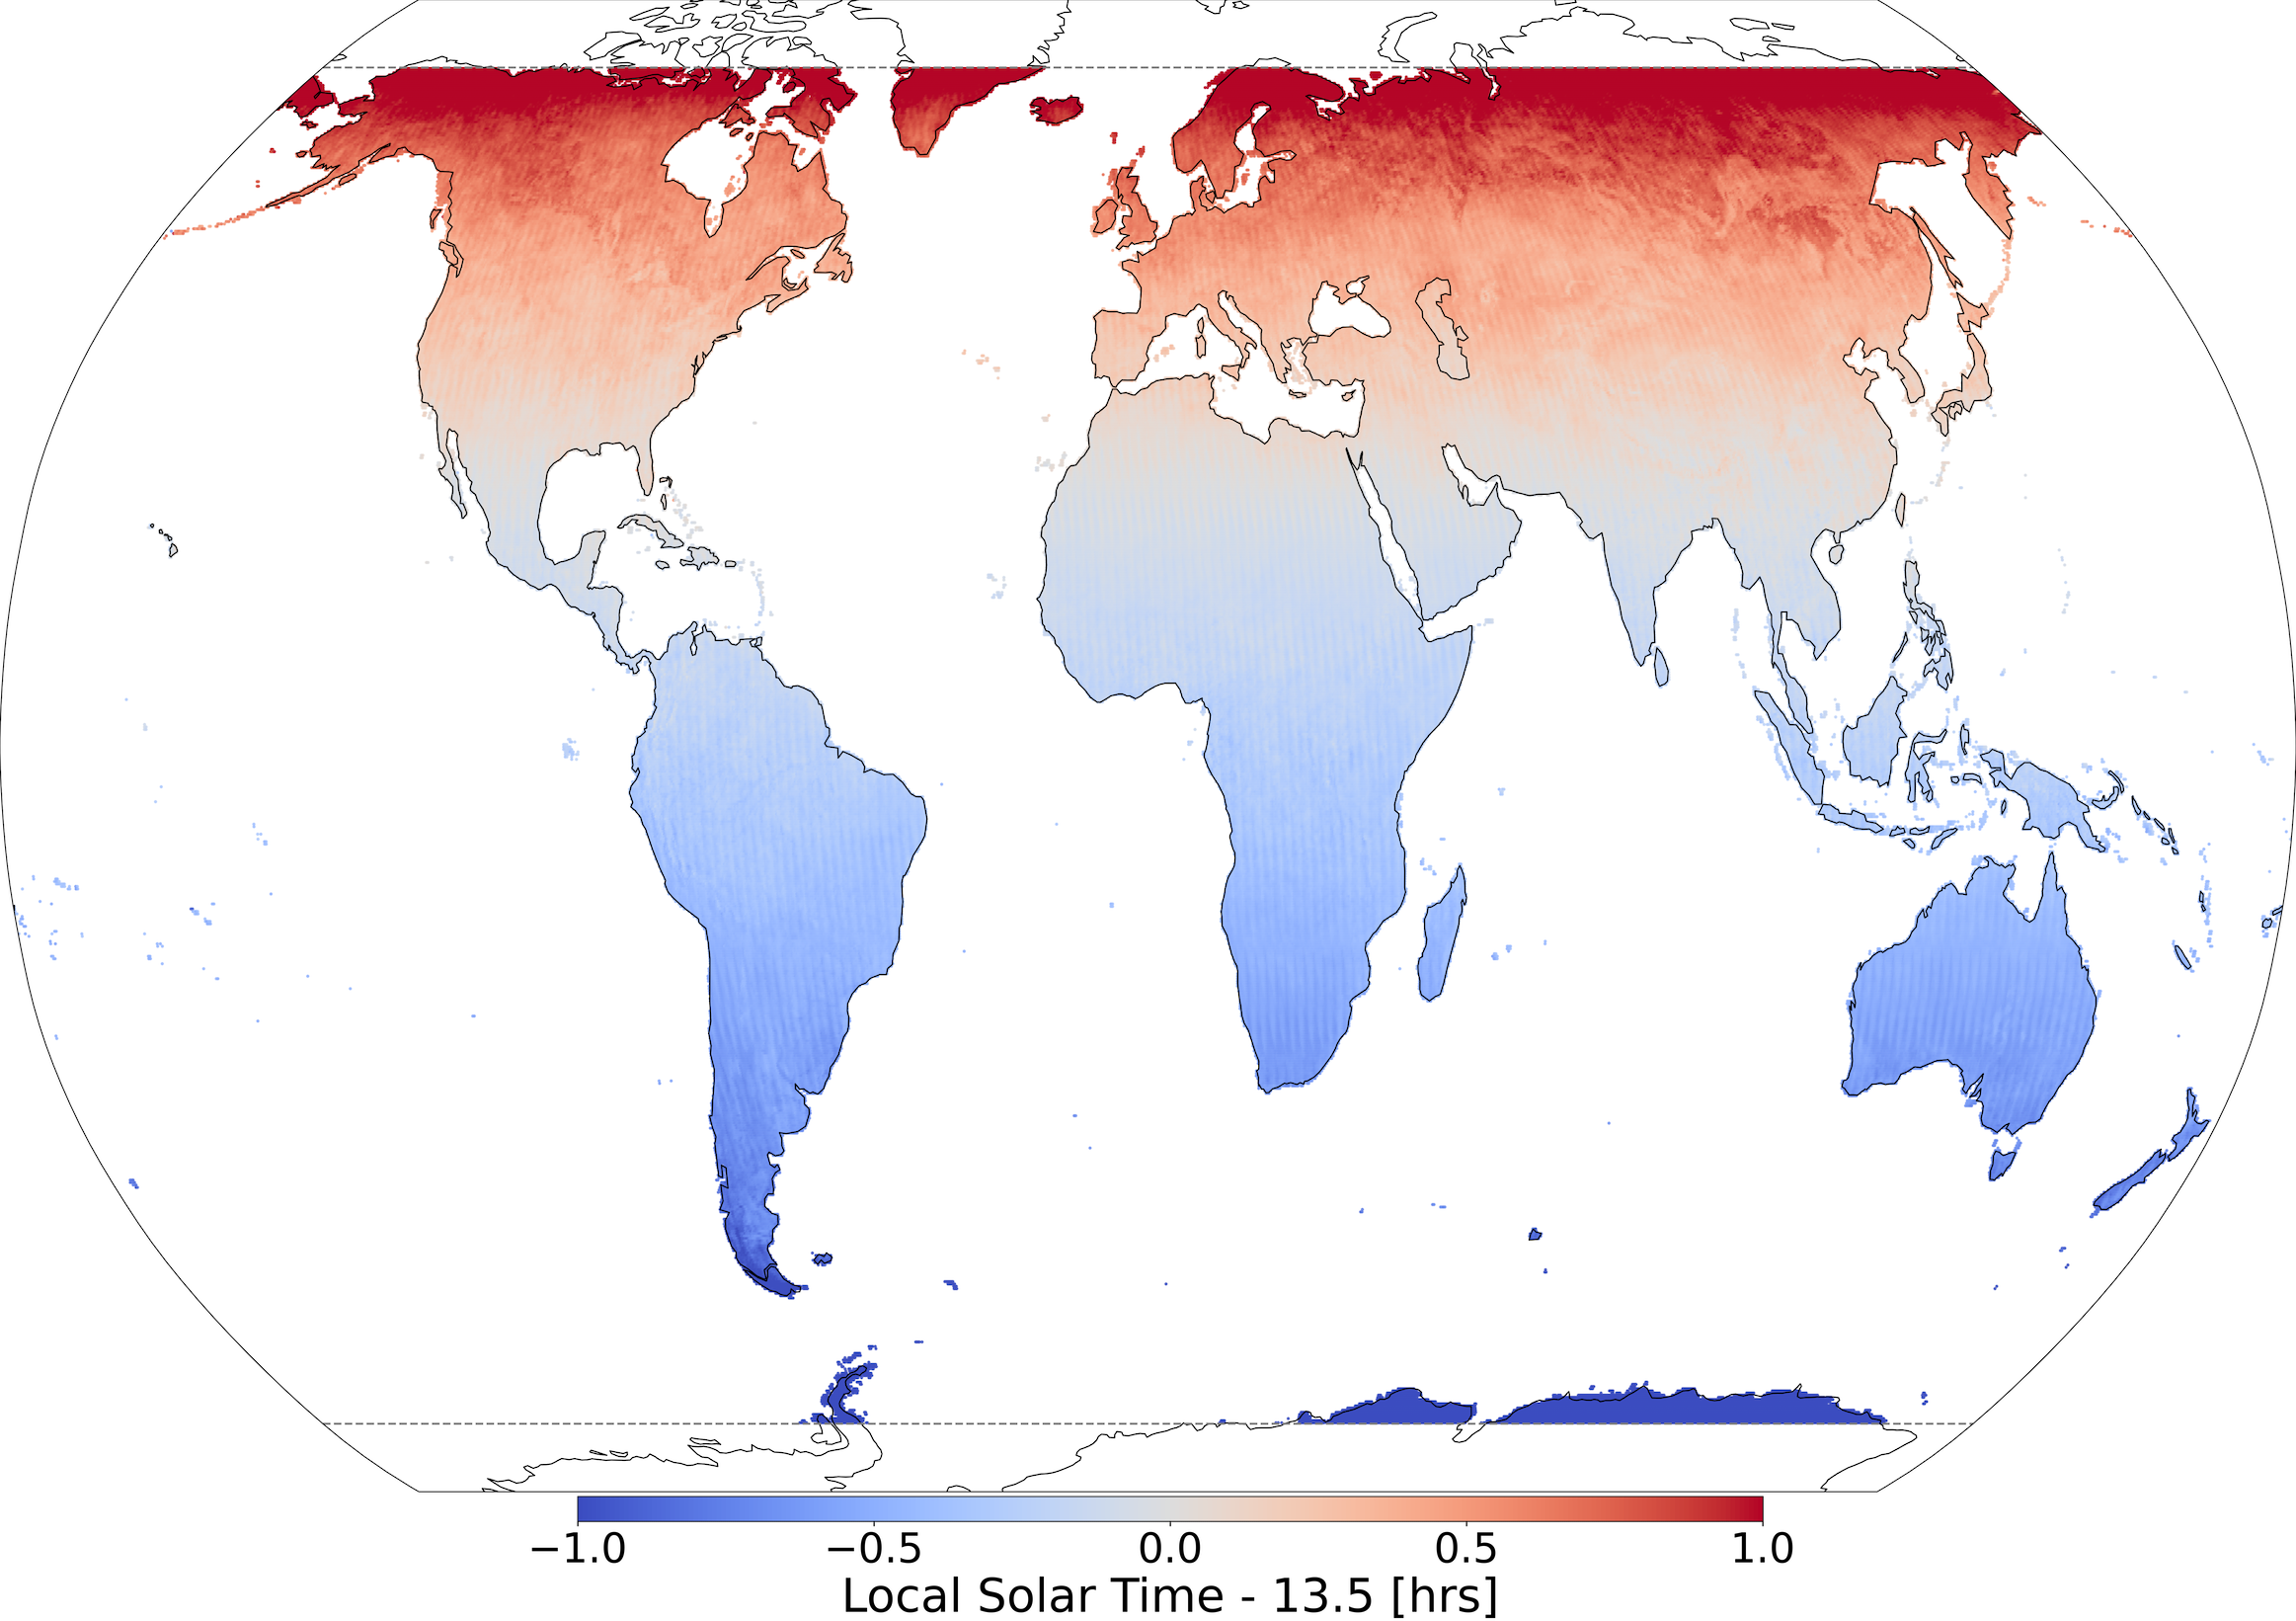
\includegraphics[width=0.48\textwidth]{MODIS_local_solar_time_diff}
	\caption{\DIFaddFL{The annually averaged mean time difference of Aqua-MODIS and assumed local solar time of 1.30pm for the year 2019 at ~31km resolution. Time differences are generally sub-hour and grow at greater latitudes, so data over 90-70°N and 70-90°S is excluded. }} 
	\label{fig:MODIS_time_error}
\end{figure}


\begin{figure}
	\subfloat[\label{fig:modis_plot_1}]{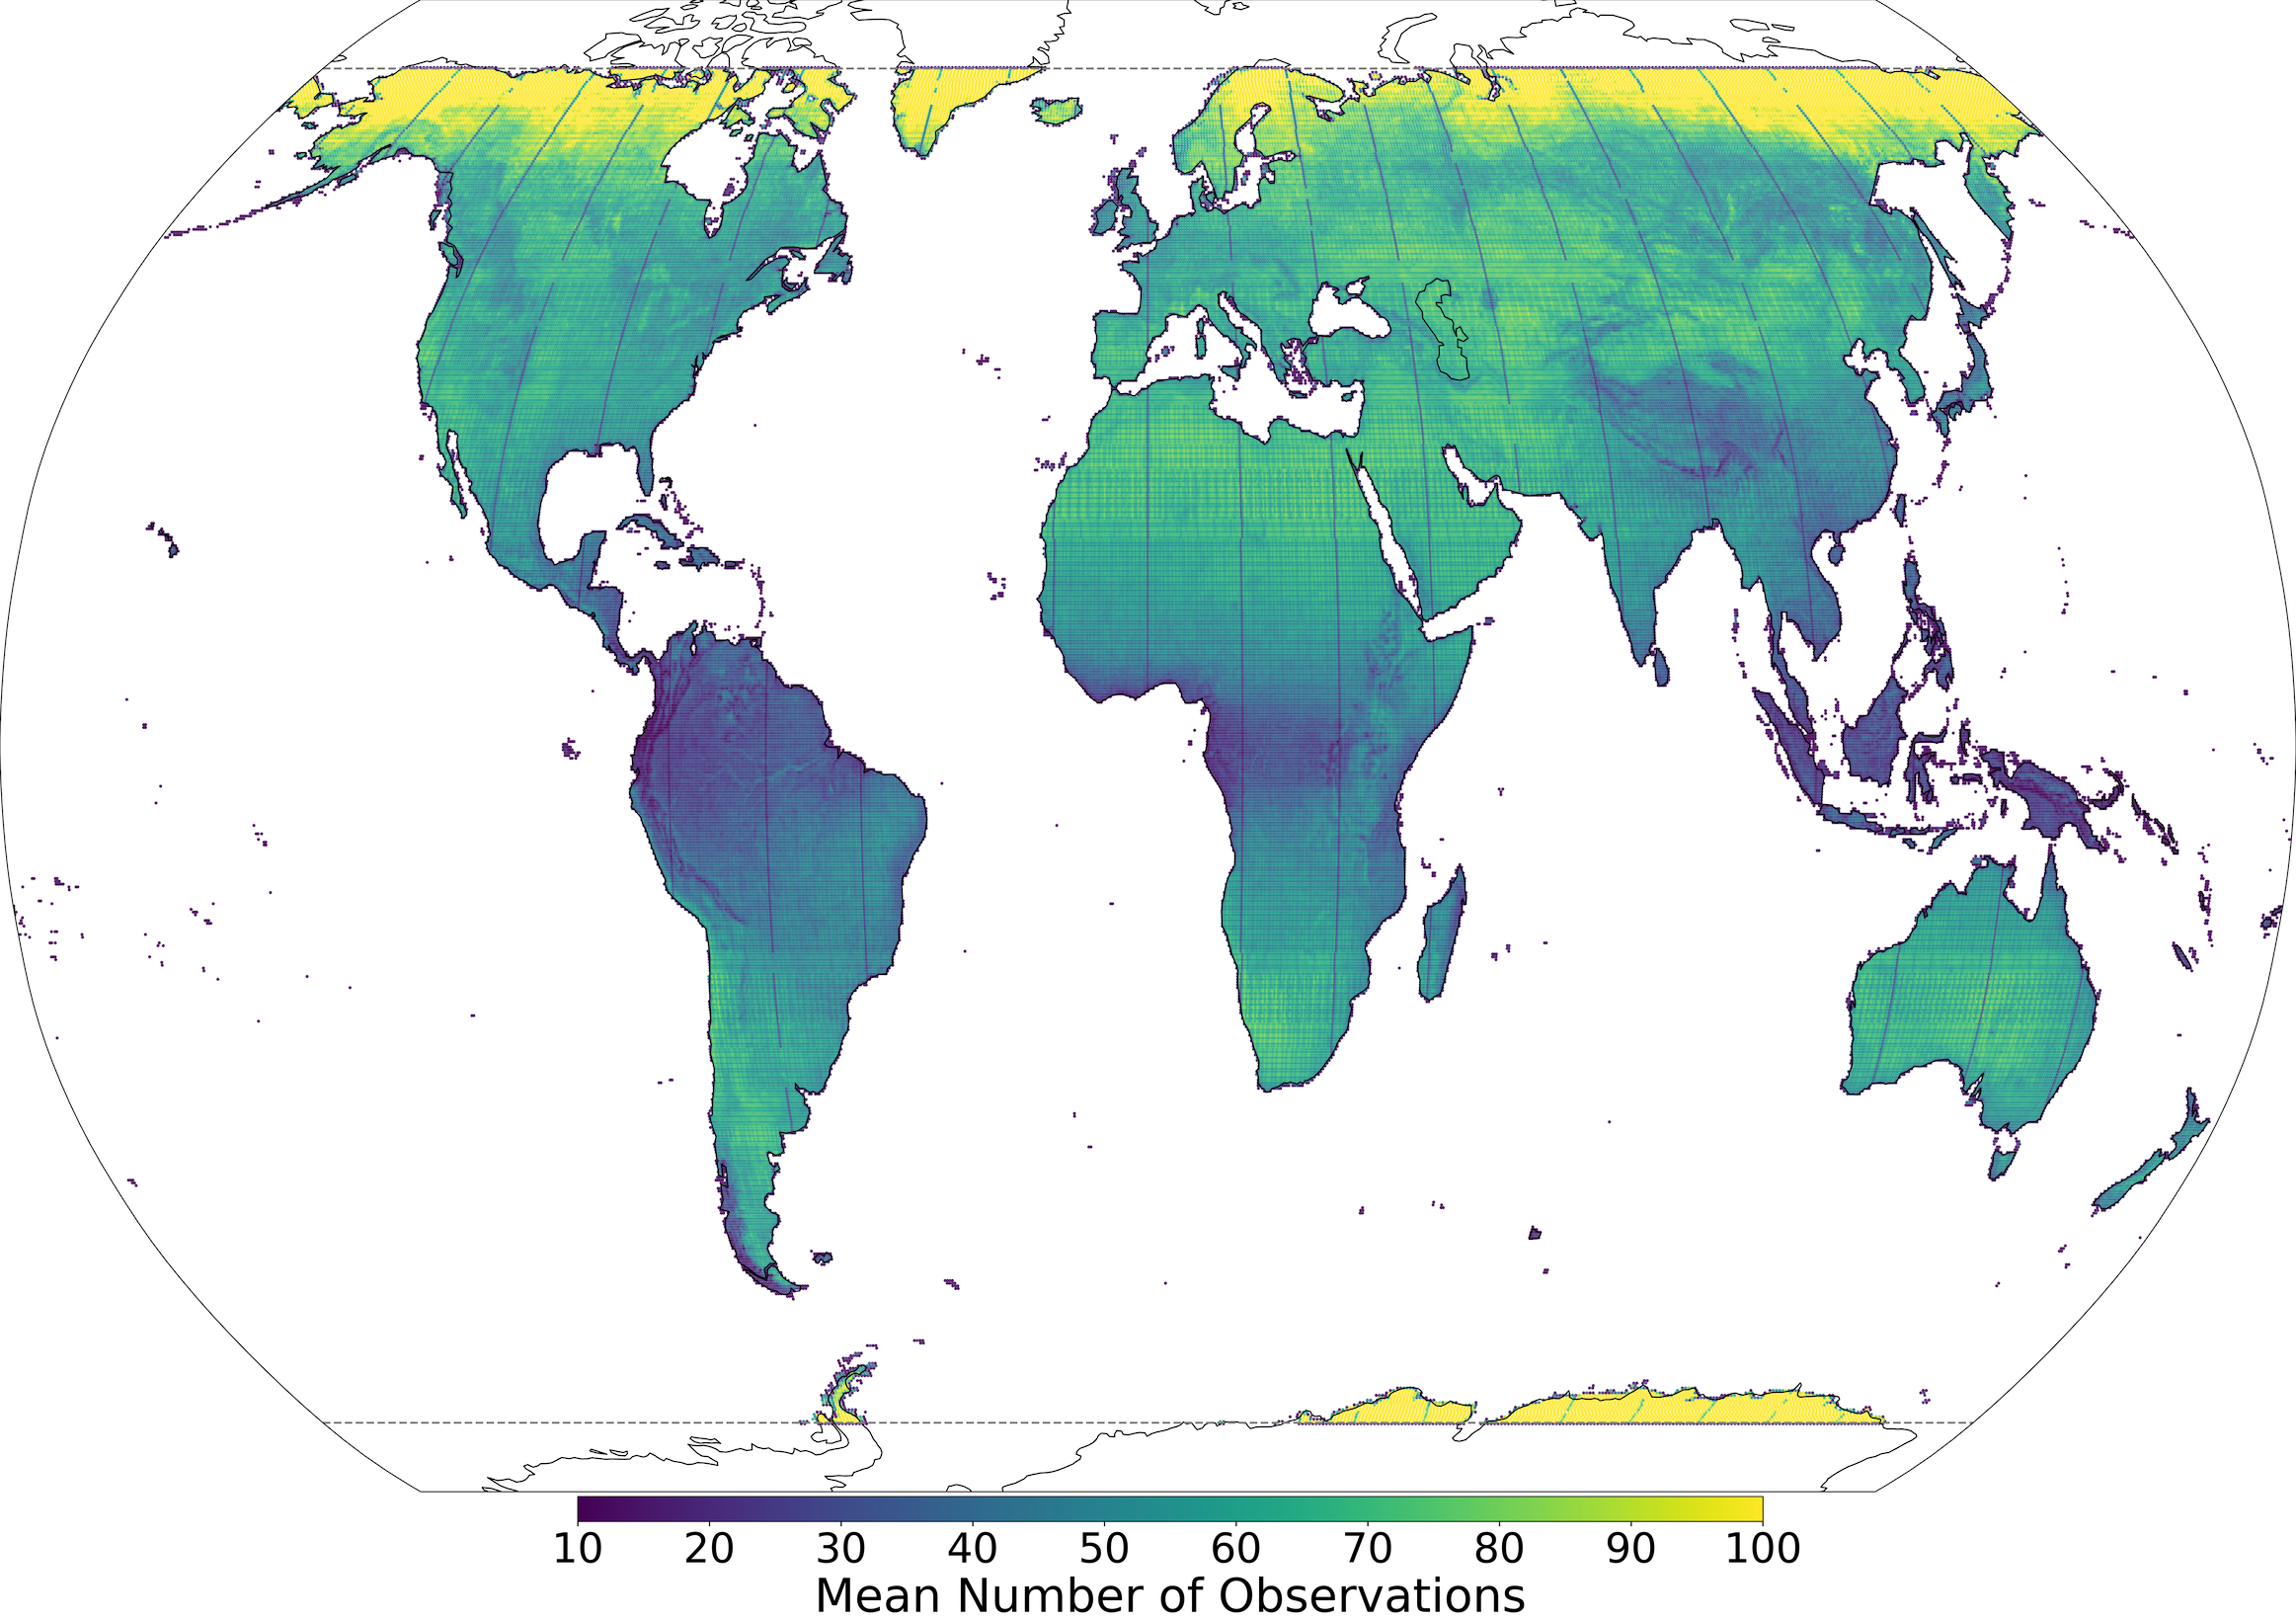
\includegraphics[width=0.48\textwidth]{num_obs_map}} \\
	\subfloat[\label{fig:modis_plot_2}]{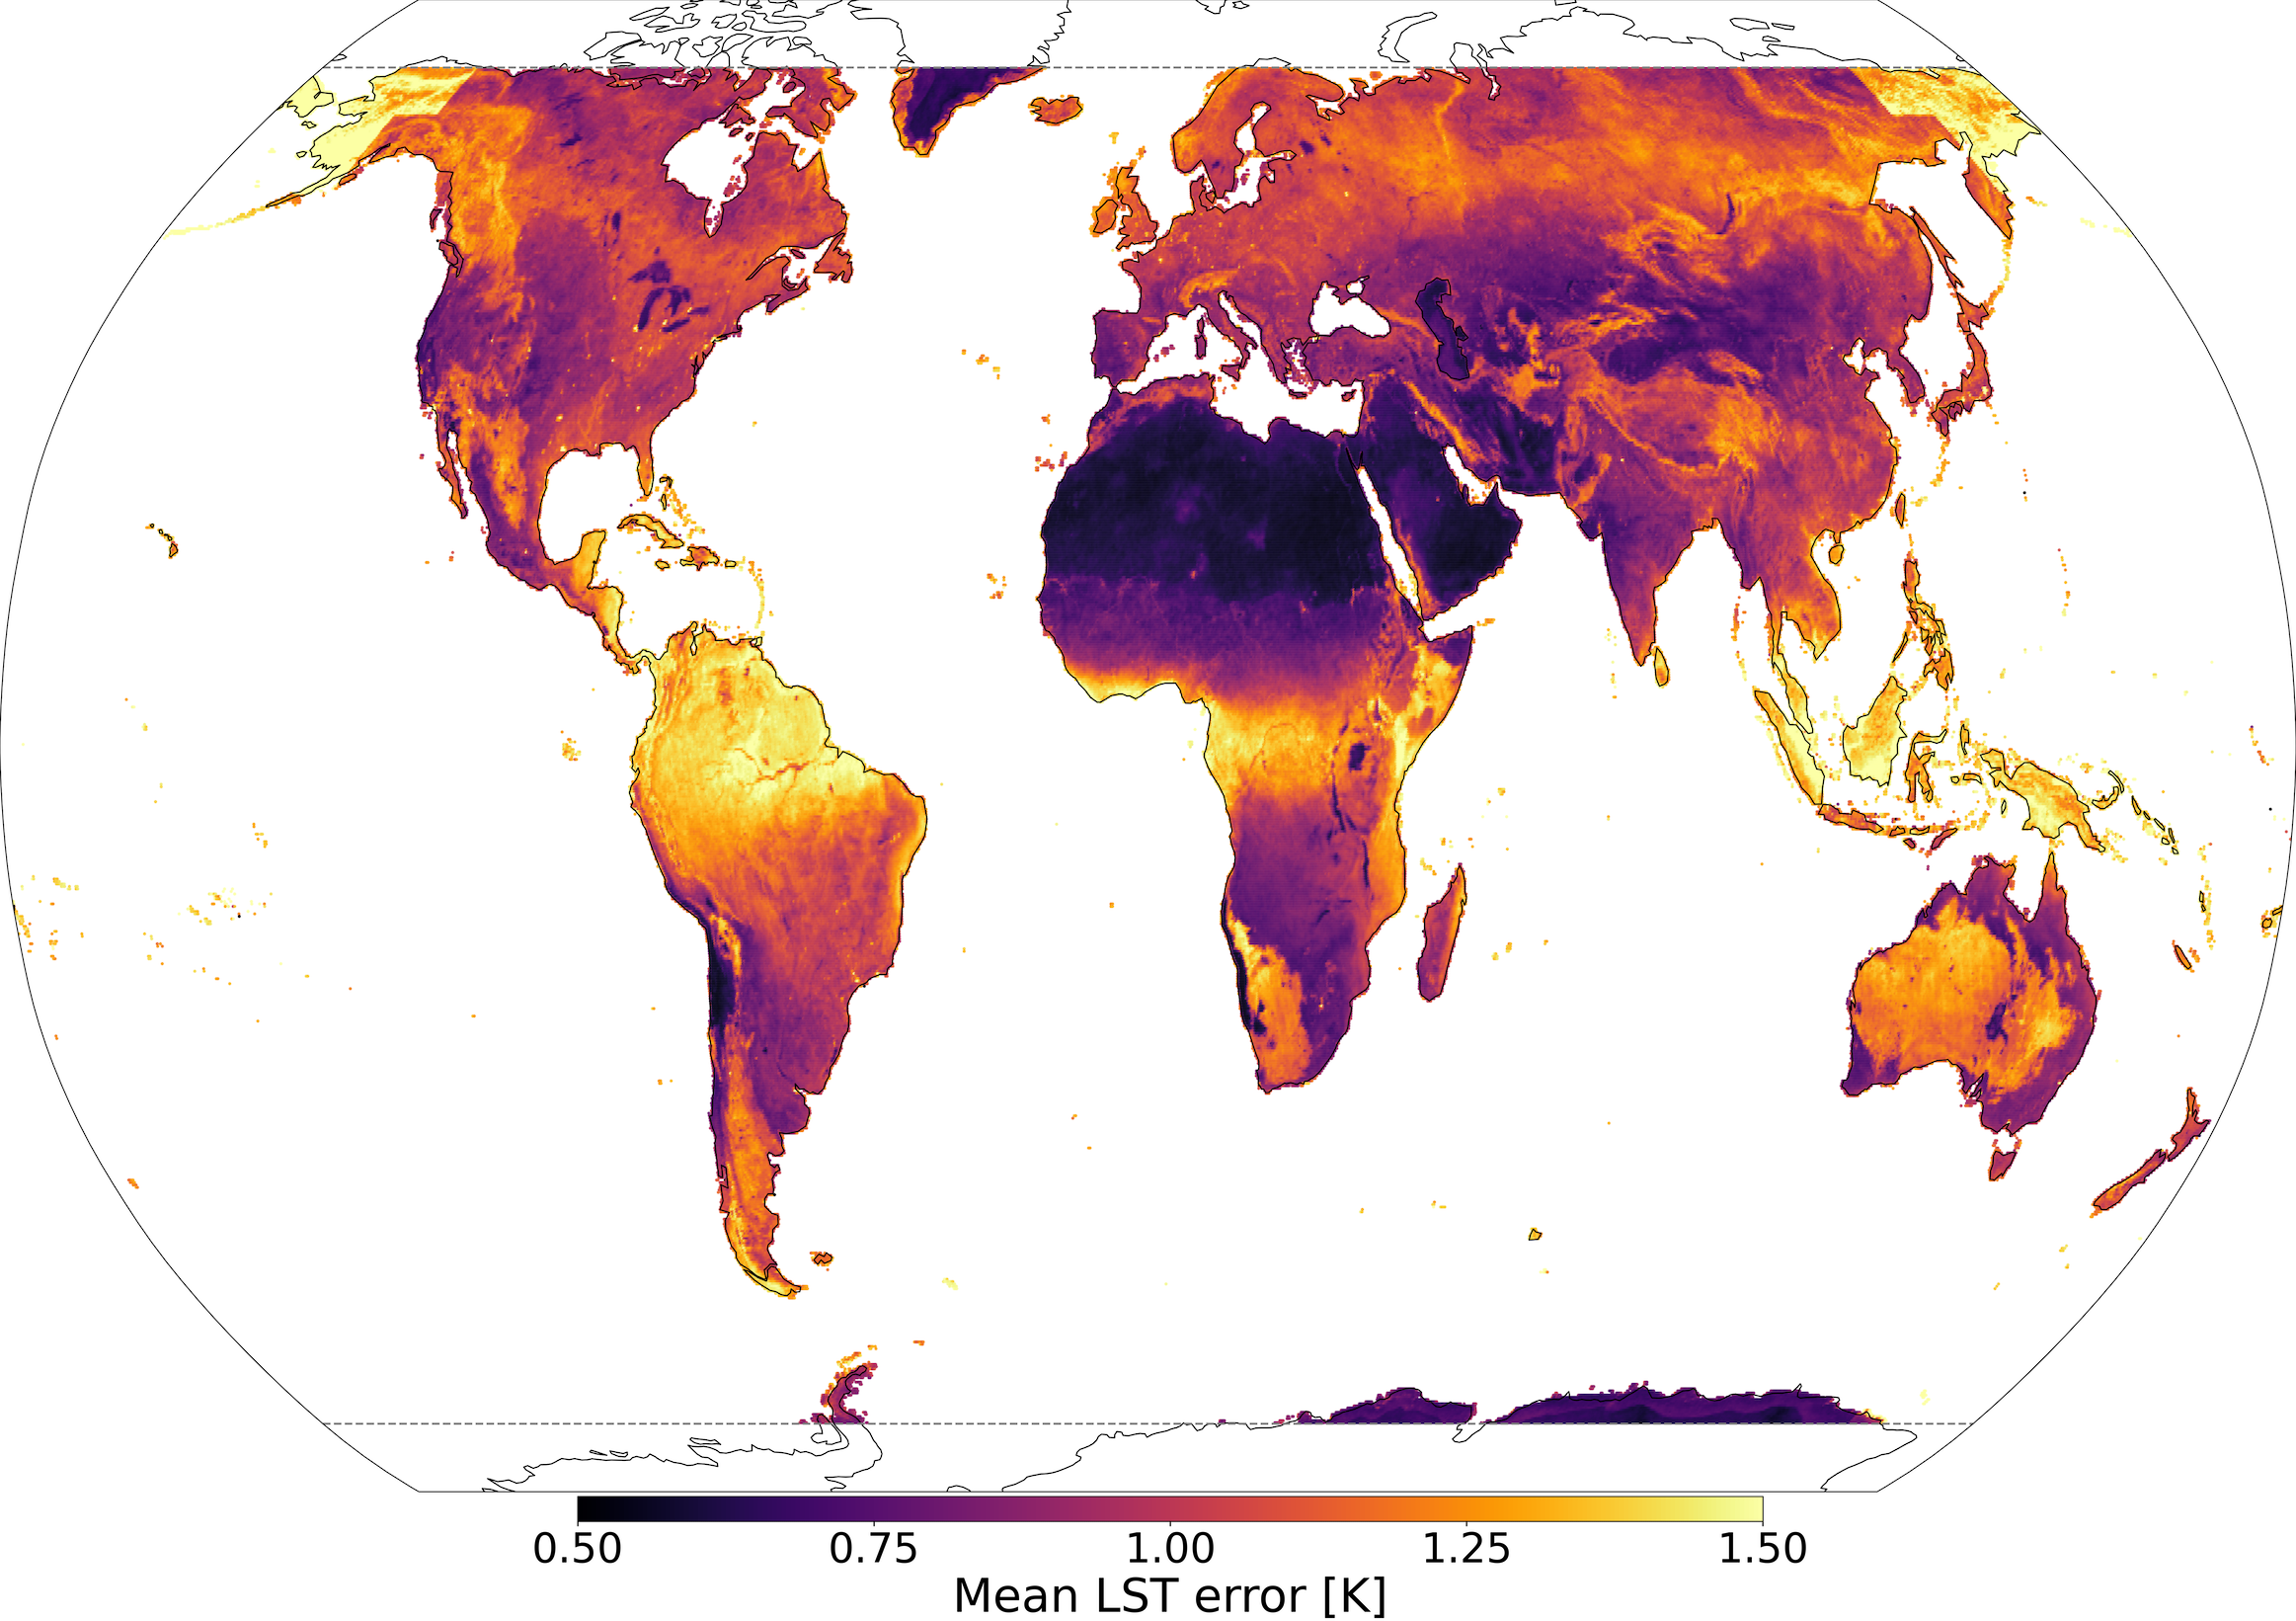
\includegraphics[width=0.48\textwidth]{MODIS_obs_error}}
	\caption{\DIFaddFL{For 2019 at $\sim$ 31km resolution: (a) Mean daily number of Aqua-MODIS observations mapped to each ERA5 data point. The swath of the Aqua satellite is clearly visible, with more observations over 70-60°N and 60-70°S areas as Aqua follows a polar orbit, south to north, and with less observations over Equator, complex orography areas (such as the Himalayas, the Andes and the Rocky Mountains), and the Siberian Tundra (due to increased cloud cover); (b) Average error in the Aqua-MODIS LST measurement. The raw Aqua-MODIS data at ~1km resolution provides categorical LST errors with bins ≤ 1K, 1-2K, 2-3K and > 3K. When averaging to the coarser resolution a weighted average over the 1km grid-cells is computed, where the median bin value is used, and 5K for the > 3K bin. This information helps to understand that abundant number of observation does not automatically mean high quality of LST (e.g. Australia).}} 
	\label{fig:MODIS_time_error_N}
\end{figure}
\noindent \DIFadd{For step (3) }\DIFaddend in \DIFdelbegin \DIFdel{our regression model. Step 2 in }\DIFdelend the joining \DIFdelbegin \DIFdel{pipeline  uses }\DIFdelend \DIFaddbegin \DIFadd{process, we use }\DIFaddend a GPU-accelerated k-nearest neighbours algorithm \cite{Rapids}, where \DIFdelbegin \DIFdel{``nearness" }\DIFdelend \DIFaddbegin \DIFadd{“nearness” on the sphere between two points }\DIFaddend is measured via the Haversine metric\DIFaddbegin \DIFadd{, }\DIFaddend i.e. the geodesic distance \DIFdelbegin \DIFdel{on the sphere between two points:
}\DIFdelend \DIFaddbegin \DIFadd{$H$, following Eq. \ref{eq:haversine}:
}\DIFaddend \begin{equation}
	H = 2 \arcsin \DIFdelbegin \DIFdel{(d)
}\DIFdelend \DIFaddbegin \left(\DIFadd{\sqrt{\sin^2\left(\frac{\delta\theta}{2}\right) + \cos \theta_1 \cos \theta_2 \sin^2\left(\frac{\delta \phi}{2}\right) }}\right)
	\label{eq:haversine}
\DIFaddend \end{equation}
\DIFdelbegin \DIFdel{where
}\begin{eqnarray*}
	\DIFdel{d = \sqrt{\sin^2\left(\frac{\delta\theta}{2}\right) + \cos \theta_1 \cos \theta_2 \sin^2\left(\frac{\delta \phi}{2}\right) }
}\end{eqnarray*}%DIFAUXCMD
%DIFDELCMD <  
%DIFDELCMD < %%%
\DIFdelend for two points with coordinate latitudes $\theta_{1,2}$, longitudes $\phi_{1,2}$ and $\delta \theta = \theta_2 - \theta_1$ and  $\delta \phi = \phi_2 - \phi_1$ . 

\DIFdelbegin %DIFDELCMD < \begin{figure}
%DIFDELCMD < 	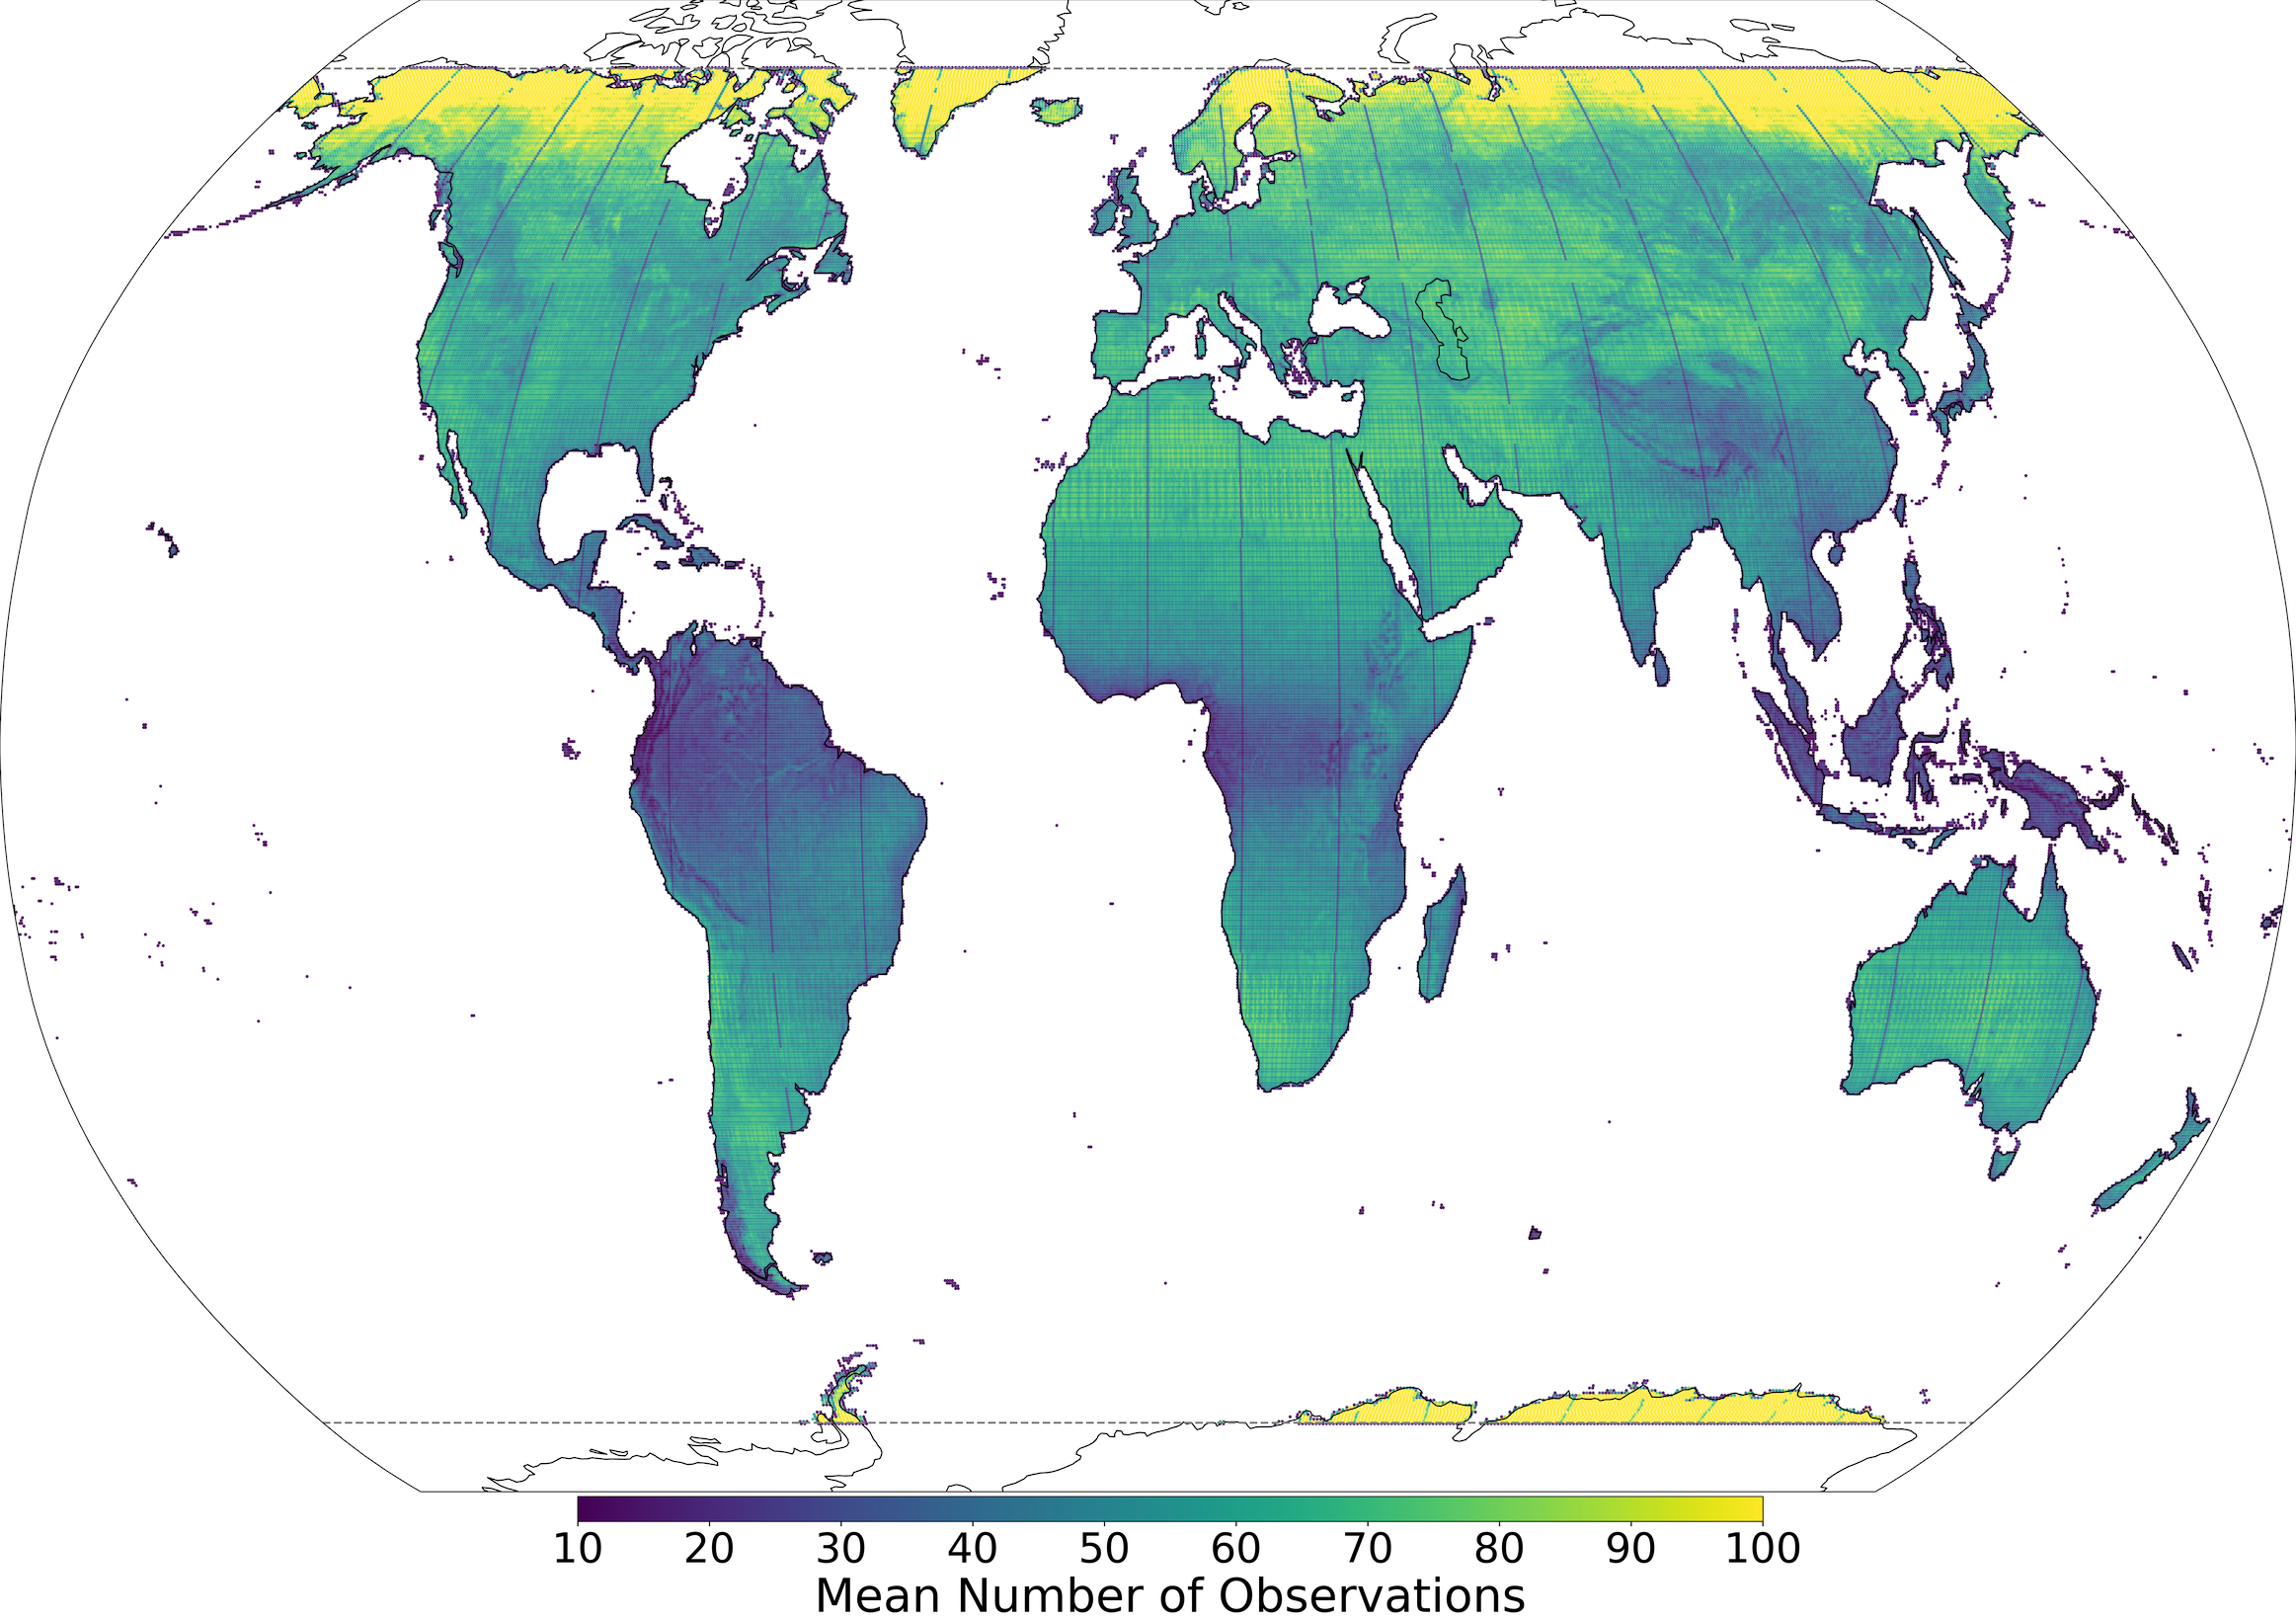
\includegraphics[width=0.48\textwidth]{num_obs_map.png}
%DIFDELCMD < 	%%%
%DIFDELCMD < \caption{%
{%DIFAUXCMD
\DIFdelFL{Mean daily number of MODIS observations mapped to each ERA5 data point for 2019. The swath of the Aqua satellite is clearly visible, with more observations at more extreme latitudes as Aqua follows a polar orbit, south to north. In addition to the expected increased sparsity of observations at the equator, there are also notably fewer observations in regions of greater orography such as the Himalayas, the Andes and the  Rocky Mountains as well as the Siberian Tundra, due to increased cloud cover.}} 
	%DIFAUXCMD
%DIFDELCMD < \label{fig:MODIS_obs}
%DIFDELCMD < \end{figure}
%DIFDELCMD < %%%
\DIFdelend 

\subsection{Constructing a regression model}
\DIFdelbegin \DIFdel{We have our features $\bar{x}$ and target $y$ data in a related format. We are now in a position to train a regression model to }\DIFdelend \DIFaddbegin \DIFadd{VESPER is trained to }\DIFaddend learn the mapping between \DIFdelbegin \DIFdel{$\bar{x}$ and }\DIFdelend \DIFaddbegin \DIFadd{features $x$ and targets }\DIFaddend $y$ \DIFdelbegin \DIFdel{. }\DIFdelend \DIFaddbegin \DIFadd{(i.e. mapping ERA5 to MODIS), a regression problem. }\DIFaddend For this purpose \DIFdelbegin \DIFdel{we use a sequential }\DIFdelend \DIFaddbegin \DIFadd{a fully-connected }\DIFaddend neural network architecture \DIFdelbegin \DIFdel{, implemented on Tensorflow \mbox{%DIFAUXCMD
\cite{tensorflow2015-whitepaper}}\hskip0pt%DIFAUXCMD
}\DIFdelend \DIFaddbegin \DIFadd{(also known as a multi-layer perceptron), implemented in Tensorflow \mbox{%DIFAUXCMD
\citep{2016arXiv160304467A} }\hskip0pt%DIFAUXCMD
was used}\DIFaddend . Whilst more advanced architectures \DIFdelbegin \DIFdel{and regression models }\DIFdelend are available, for \DIFdelbegin \DIFdel{our purposes the sequential model is more than sufficient and it }\DIFdelend \DIFaddbegin \DIFadd{the purposes of this work the model is sufficient enough, which }\DIFaddend exhibits generally fast and dependable convergence. \DIFdelbegin \DIFdel{We take as our canonical structure a network where the }\DIFdelend \DIFaddbegin \DIFadd{The networks built have differing }\DIFaddend number of nodes in the input layer\DIFdelbegin \DIFdel{is equal to }\DIFdelend \DIFaddbegin \DIFadd{, depending on }\DIFaddend the number of \DIFdelbegin \DIFdel{training features, a single node in the output layer corresponding to the LST and }\DIFdelend \DIFaddbegin \DIFadd{predictors (see Table \ref{tab:vesper_table}). For all networks constructed we use }\DIFaddend 4 hidden layers \DIFdelbegin \DIFdel{where the number of nodes in each layer is equal to the half the number of input nodes. For our optimisation schemewe use ADAM\mbox{%DIFAUXCMD
\cite{2014adam} }\hskip0pt%DIFAUXCMD
and set the learning rate }\DIFdelend \DIFaddbegin \DIFadd{and a layer width is half that of the input layer width. ADAM \mbox{%DIFAUXCMD
\citep{2014adam} }\hskip0pt%DIFAUXCMD
is used as an optimisation scheme, learning rate is set }\DIFaddend to $3 \times 10^{-4}$, and \DIFaddbegin \DIFadd{default values for }\DIFaddend the exponential decay rate for the 1st and 2nd moment estimates \DIFdelbegin \DIFdel{take default values of $0.90$ and $0.999$}\DIFdelend \DIFaddbegin \DIFadd{are set to 0.900 and 0.999 respectively}\DIFaddend . The network is not trained for a fixed number of epochs, but instead trained until the validation error reaches a minimum. Techniques for maximising the performance of a network via hyperparameter optimisation are now well established \DIFdelbegin \DIFdel{\mbox{%DIFAUXCMD
\cite{HPO1,HPO2}}\hskip0pt%DIFAUXCMD
. Howeverfor our purposes we do not try in any meaningful way to tune our hyperparameters , instead just take }\DIFdelend \DIFaddbegin \DIFadd{\mbox{%DIFAUXCMD
\citep{HPO2,HPO1}}\hskip0pt%DIFAUXCMD
. However, for the purposes of this work no attempt to tune hyperparameters was made, just }\DIFaddend some reasonable default values \DIFdelbegin \DIFdel{which we judge to be ``good enough''. Some shallow }\DIFdelend \DIFaddbegin \DIFadd{were applied which were assumed to be “good enough”. Some }\DIFaddend exploration of different hyperparameter configuration was undertaken, but for this data the prediction accuracy is mostly independent of the hyperparameter configuration, subject to standard and reasonable hyperparameter choices. Whilst a more advanced automatic hyperparameter optimization method may have enabled slightly \DIFdelbegin \DIFdel{more performance to be squeezed out of the model}\DIFdelend \DIFaddbegin \DIFadd{higher performance of VESPER}\DIFaddend , our ultimate purpose is not to generate the most absolutely accurate prediction possible, but instead to have two predictive models which \DIFdelbegin \DIFdel{we can compare. Additionally, as we will see, }\DIFdelend \DIFaddbegin \DIFadd{can be compared. In the result section below it will be shown that }\DIFaddend the variation in performance due to \DIFdelbegin \DIFdel{modifications to the input features }\DIFdelend \DIFaddbegin \DIFadd{input feature modifications }\DIFaddend is far greater than the variation due to the hyperparameter choices. \newline 

 \noindent \DIFdelbegin \DIFdel{With a fully trained network we can then deploy the model to make predictions of the LST over the whole globe. An example of the error in the predicted LST relative to the true MODIS LST, is presented  in Figure \ref{fig:example_model}. The model }\DIFdelend \DIFaddbegin \DIFadd{VESPER }\DIFaddend was trained on \DIFdelbegin \DIFdel{a year of }\DIFdelend \DIFaddbegin \DIFadd{selected atmospheric and surface model fields from }\DIFaddend ERA5 \DIFdelbegin \DIFdel{data from 2016 and then made predictions of the LST in }\DIFdelend \DIFaddbegin \DIFadd{for 2016 (see Table \ref{table:definitions}), certain static version of the surface physiographic fields (see Table \ref{tab:datasources}), and Aqua-MODIS LST for 2016. Once VESPER was fully trained it was used to predict LST over the whole globe for }\DIFaddend 2019. \DIFdelbegin \DIFdel{We can compare the error in the model predictions with the error in the predicted skin temperature that is derived }\DIFdelend \DIFaddbegin \DIFadd{Going forward, as a shorthand we will refer to VESPER trained using the e.g. $V15$ field set as VESPER\_V15 (in general VM is a field set version and VESPER\_VM is a VESPER model trained using the fields }\DIFaddend from \DIFaddbegin \DIFadd{the VM field set). See Table \ref{tab:vesper_table} for an explicit definition of all the VESPER models. The training and test years were chosen simply as recent, non-anomalous years so that the updated  surface physiographic fields could be checked. All VESPER versions are trained with }\DIFaddend ERA5 \DIFdelbegin \DIFdel{. It is evident from Figure \ref{fig:example_model} that the trained model generally enjoys increased accuracy over the }\DIFdelend \DIFaddbegin \DIFadd{fields for 2016 and with main surface physiographic fields from V15 field set. Then depending on the version some or all additional surface physiographic fields (see Table \ref{table:definitions}) are added. VESPER’s predictions can be compared to the initial }\DIFaddend ERA5 \DIFdelbegin \DIFdel{predictions, }\DIFdelend \DIFaddbegin \DIFadd{skin temperatures and actual Aqua-MODIS LST for 2019. Figure \ref{fig:example_model} shows the mean absolute errors (MAE) globally in the VESPER\_V15 LST predictions, relative to the Aqua-MODIS LST along with the corresponding MAE in the predicted skin temperature from ERA5. We can see that VESPER\_V15 was able to learn corrections to ERA5, }\DIFaddend especially in the Himalayas and sub-Saharan \DIFdelbegin \DIFdel{Africa as well as Australia and the Amazon basin. For this particular example, the mean annual error, averaged over all grid points was }\DIFdelend \DIFaddbegin \DIFadd{Africa as well as Australia and the Amazon basin, leading to the globally averaged MAE reduction for predicted LST; the MAE relative to  Aqua-MODIS LST, averaged over all grid points, was }\DIFaddend 3.9\DIFdelbegin \DIFdel{K for the ERA5 prediction and 3.0 }\DIFdelend K for \DIFdelbegin \DIFdel{the model prediction. This serves as a useful sanity check to give us confidence that the network is performing as expected and gives generally reasonable predictive performance, at least as good - if not better - than then derived skin temperature predictions from }\DIFdelend ERA5 \DIFdelbegin \DIFdel{. More fundamentally, this also indicates that there is some information captured in the input fields to the network that is not expressed through the current ERA5 reanalysis modelling.This again motivates the development of updated parametrization schemes that better represent small scale processes and better capture this information. }%DIFDELCMD < \newline
%DIFDELCMD < 

%DIFDELCMD < \begin{figure*}
%DIFDELCMD < 	\subfloat[\label{fig:wasserstein_temperature}]{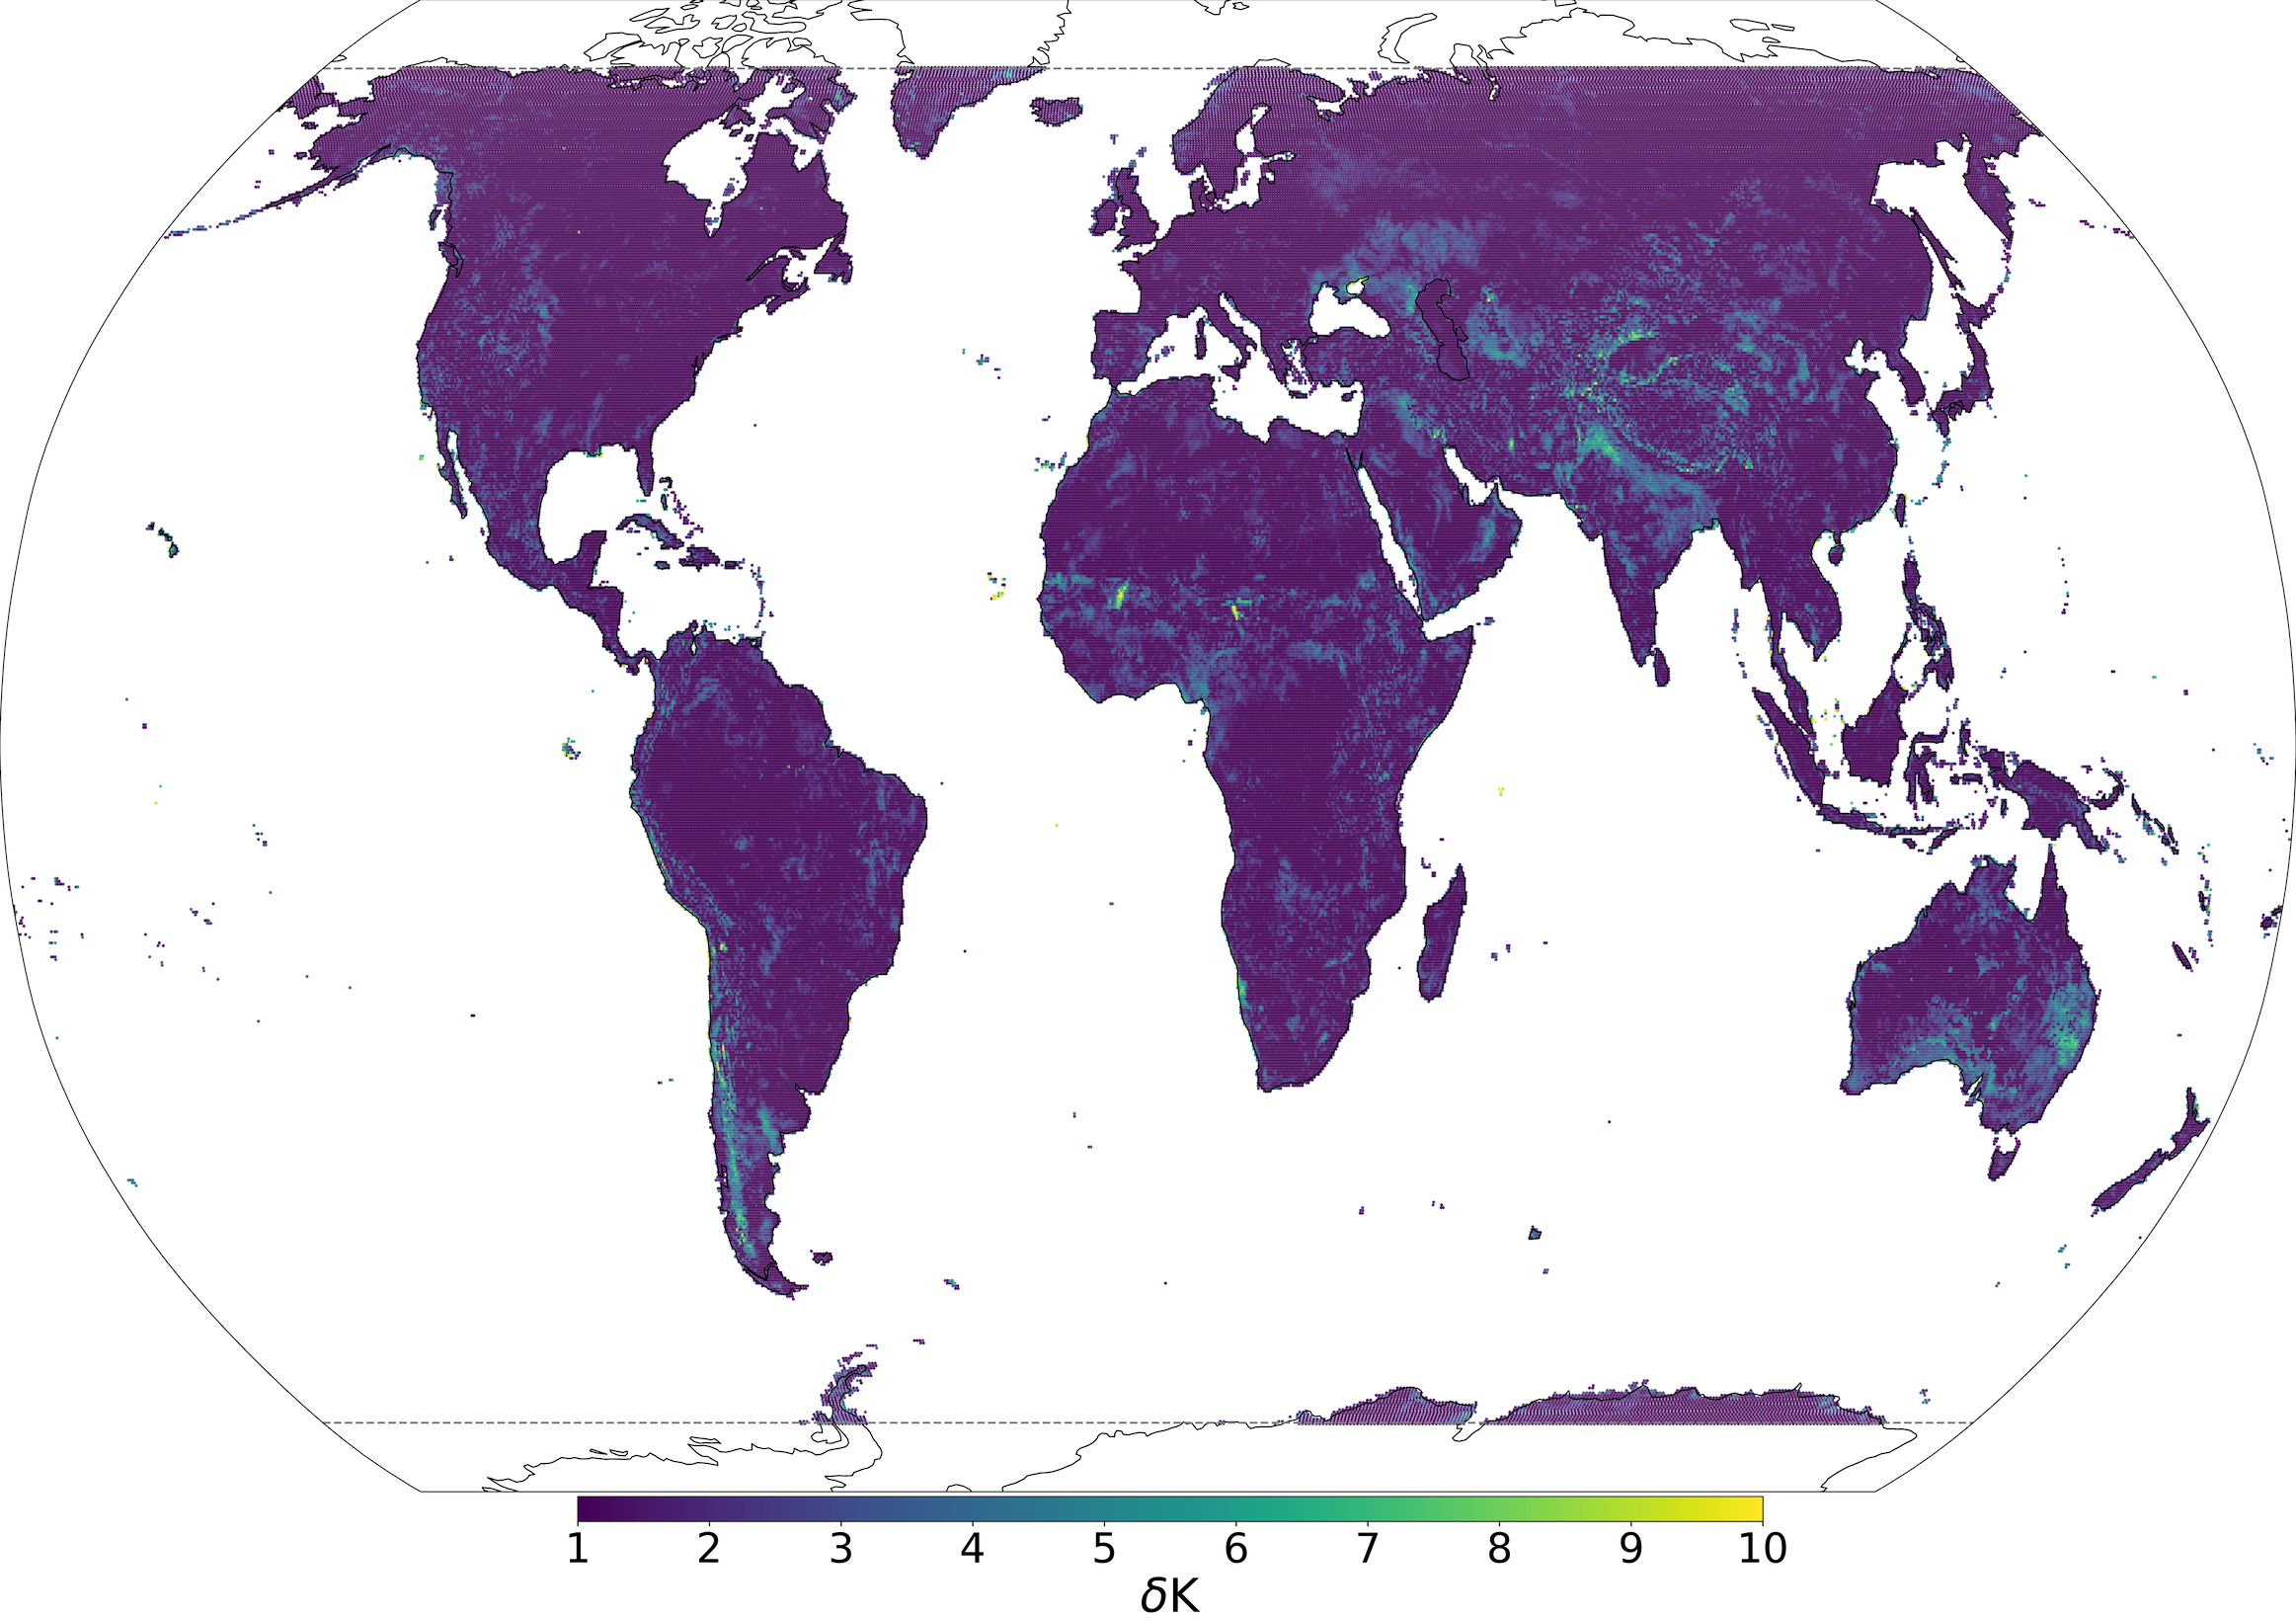
\includegraphics[width=0.48\textwidth]{model_prediction_error.png}} %%%
\DIFdelFL{\hspace{1mm}
	}%DIFDELCMD < \subfloat[\label{fig:wasserstein_precipitation}]{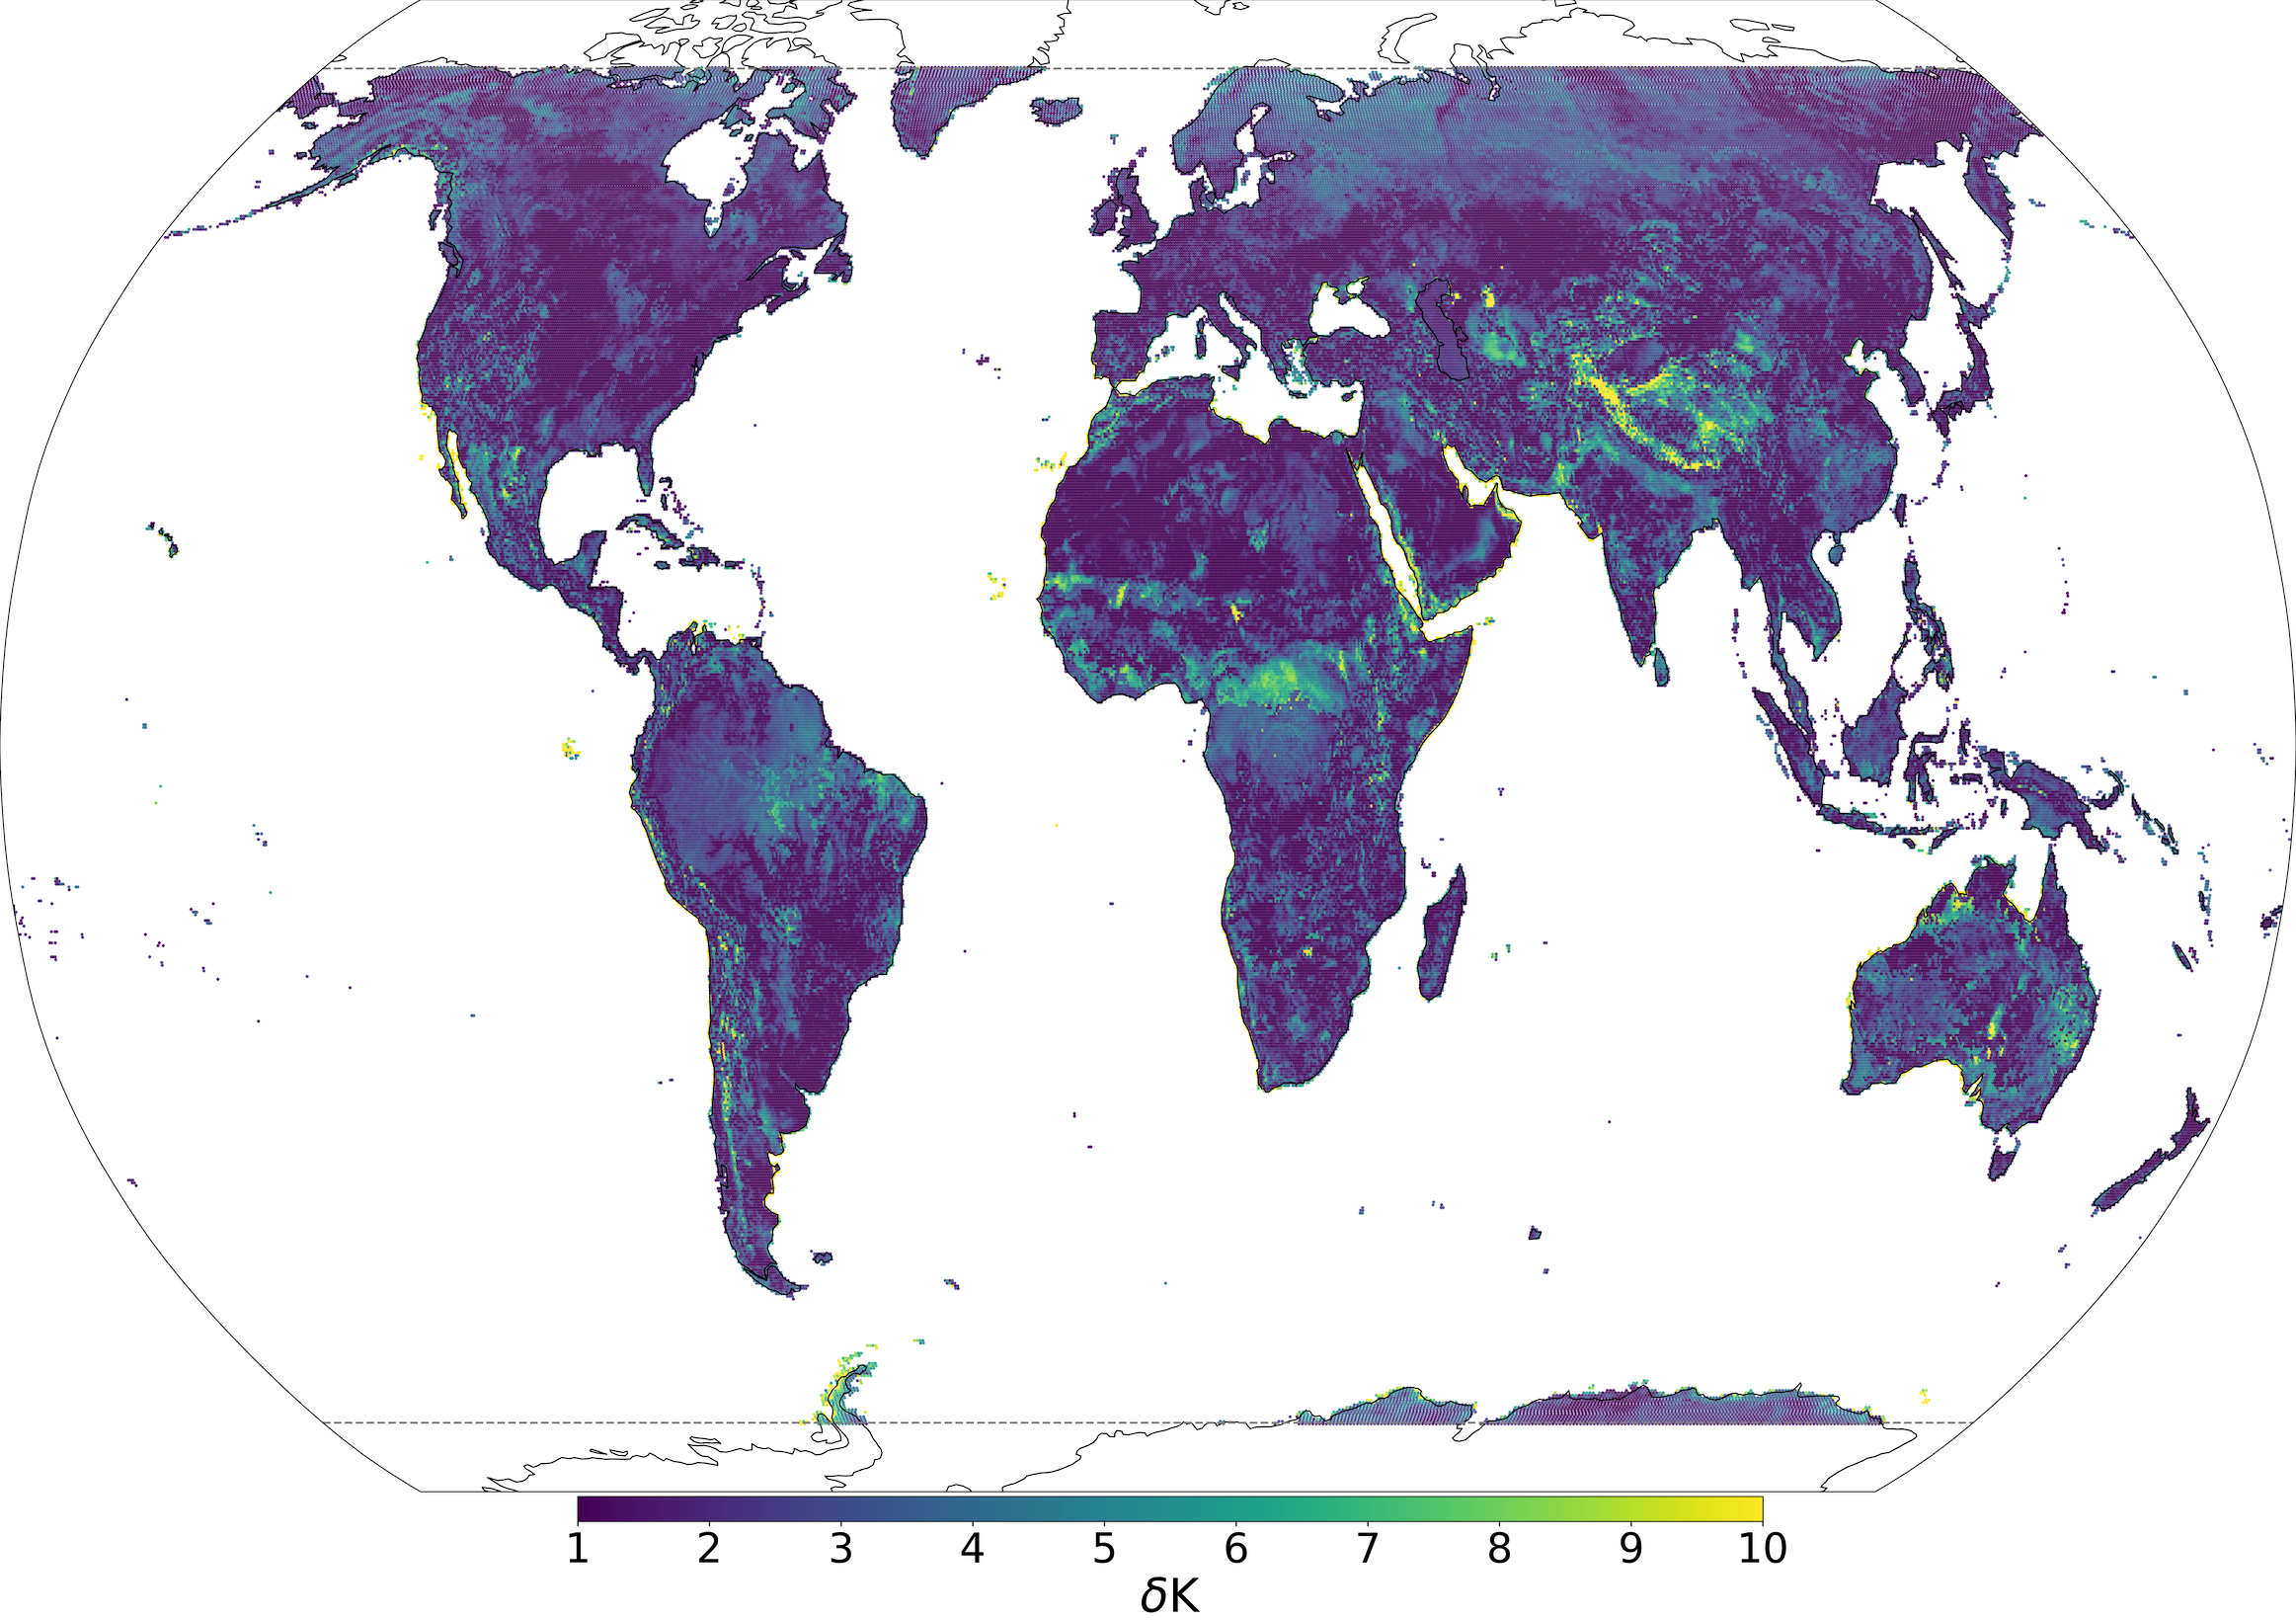
\includegraphics[width=0.48\textwidth]{ERA_prediction_error.png}}
%DIFDELCMD < 	%%%
%DIFDELCMD < \caption{%
{%DIFAUXCMD
\DIFdelFL{Prediction error relative to MODIS Aqua observations in the land surface temperature  ($\delta K$) for 2019, averaged over the year, for }\textit{\DIFdelFL{(a)}} %DIFAUXCMD
\DIFdelFL{Trained Neural Network and }\textit{\DIFdelFL{(b) }}%DIFAUXCMD
\DIFdelFL{ERA5. It can be seen that the network generally outperforms the ERA5 predictions, which generally struggles in regions with complex surface fields such as the Himalayas (lots of orography) sub-Saharan Africa (lots of vegetation) and the Amazon Basin (lots of water + vegetation). In contrast the network demonstrates generally good performance, with some drop off in the Himalayas and the eastern cost of Australia, but still outperforming ERA5.}} 
	%DIFAUXCMD
%DIFDELCMD < \label{fig:example_model}
%DIFDELCMD < \end{figure*}
%DIFDELCMD < 

%DIFDELCMD < %%%
\section{\DIFdel{Evaluating Updated Lake Fields}}%DIFAUXCMD
\addtocounter{section}{-1}%DIFAUXCMD
%DIFDELCMD < \label{sec:3}
%DIFDELCMD < %%%
\DIFdel{As discussed, at ECMWF parametrised lake representation in the IFS is handled by FLake.The primary physiographic dataset used in the IFS to generate the lake parameters is the GlobCover2009 global map  \mbox{%DIFAUXCMD
\cite{GLOBCOVER}}\hskip0pt%DIFAUXCMD
\mbox{%DIFAUXCMD
\cite{arino2012glcm}}\hskip0pt%DIFAUXCMD
. This map has a resolution of 300m and covers latitudes from $60^{\circ}$S to $85^{\circ}$N; corrections outside this latitude band for the polar regions and Iceland are included separately.  In the Arctic no land is assumed, whilst in the Antarctic data from version 2 of the Radarsat Antarctic Mapping Project (RAMP2) digital elevation model (DEM) is used\mbox{%DIFAUXCMD
\cite{Liu2015}}\hskip0pt%DIFAUXCMD
. For Iceland, data from the Digital map database of Iceland (IS 50V) is used. }%DIFDELCMD < \newline 
%DIFDELCMD < 

%DIFDELCMD < \noindent %%%
\DIFdel{More recently, new datasets and methods for updating the lake fields for the IFS have been proposed\mbox{%DIFAUXCMD
\cite{Choulga2019}}\hskip0pt%DIFAUXCMD
. These new datasets include the Global Surface Water Explorer (GSWE) dataset from the Joint Research centre (JRC)\mbox{%DIFAUXCMD
\cite{GSWE}}\hskip0pt%DIFAUXCMD
. GSWE is a 30m resolution dataset from Landsat 5,7 }\DIFdelend and \DIFdelbegin \DIFdel{8, providing  information on the spatial and temporal variability of surface water on the Earth since March 1984. This then allowed for particular geographical regions to be updated with more up-to-date, high resolution data, providing additional information that is not captured by GlobCover2009. Whilst multiple lake areas were updated based on this new data, particularly noteworthy regions include:
}%DIFDELCMD < \begin{itemize}
\begin{itemize}%DIFAUXCMD
%DIFDELCMD < 	\item %%%
\item%DIFAUXCMD
\textbf{\DIFdel{Aral Sea}}%DIFAUXCMD
\DIFdel{. The Aral Sea lies across the border between Uzbekistan and Kazakhstan and was at one point the 4th largest lake in the world. However, the Aral Sea has long been shrinking, at an accelerated rate since the 1960s. It started to stabilise in 2014 with an area of $7660 \text{km}^2$, 9 times smaller than its size in 1960, and its eastern basin is now known as the Aralkum Desert. The water map from GlobCover2009 describes the Aral Sea in 1998, when it was still ``only" 2 times smaller than its 1960 extent, whereas GSWE provides a more up to date map. }%DIFDELCMD < \item %%%
\item%DIFAUXCMD
\textbf{\DIFdel{Australia}}%DIFAUXCMD
\DIFdel{. GlobCover2009 over-represents inland water in Australia, which generally has a huge number of lakes. However, some of these lakes are highly ephemeral;  the endorheic Kati Thanda–Lake Eyre fills only a few times per century. The GSWE updates to this region therefore include only generally permanent water, removing all seasonal and rare ephemeral water. 
}
\end{itemize}%DIFAUXCMD
%DIFDELCMD < \end{itemize} 
%DIFDELCMD < %%%
\DIFdel{The lake depth is not specified by GlobCover2009/GSWE, instead being described by the Global Lake DataBase (GLDB) \mbox{%DIFAUXCMD
\cite{Kourzeneva2012}}\hskip0pt%DIFAUXCMD
. Lake depth is recognized as being an important field in the IFS, since over estimates can result in strong cold biases in hotter seasons or else a lack of ice formation. Under the program to continuously update the parametrisation schemes, recently the original version of the dataset, GLDBv1,with coarse resolution aggregation technique MEAN, has been superseded by GLDBv3\mbox{%DIFAUXCMD
\cite{Choulga2014}}\hskip0pt%DIFAUXCMD
, with coarse resolution aggregation technique MODE. GLDBv3 increases the total number of lakes with in situ information by $\sim1500$, introduces a depth distinction between freshwater and saline lakes, and updates the method by which the lake depth is calculated based on climate type and geological origins. Consequently, whilst the updated fields when going from GlobCover2009 to GSWE applied at particular geographic regions, the lake depth field is generally updated globally. Verification of the updated lake depth fields against 353 lakes in Finland shows that GLDBv3 exhibits a 52$\%$ bias reduction compared to GLDBv1\mbox{%DIFAUXCMD
\cite{Choulga2019}}\hskip0pt%DIFAUXCMD
. For a thorough discussion of the upgraded lake fields, the lake depth, and the representation of lakes generally by ECMWF we refer the reader to\mbox{%DIFAUXCMD
\cite{Choulga2019,Boussetta2021}}\hskip0pt%DIFAUXCMD
. }\DIFdelend \DIFaddbegin \DIFadd{3.0K for VESPER\_V15. }\DIFaddend \newline 

 \DIFdelbegin %DIFDELCMD < \noindent %%%
\DIFdel{This distinction between the original lake maps based on GlobCover2009 and GLDBv1 data and the updated lake maps which have been corrected using GSWE and GLDBv3 data provides an ideal test bed to deploy and demonstrate our tool. Can we use VESPERto evaluate the added value of these new fields? 
}%DIFDELCMD < 

%DIFDELCMD < %%%
\subsection{\DIFdel{V15 vs V20}}
%DIFAUXCMD
\addtocounter{subsection}{-1}%DIFAUXCMD
%\DIFdel{In order to ascertain the accuracy and information content of the updated lake fields we will proceed as follows. We will train two permutations of the regression model, one where the }\DIFdelend \DIFaddbegin \begin{table*}
% 	\begin{tabularx}{\textwidth}{lXXXX}
% 		\toprule
% 		\DIFaddFL{Model }& \DIFaddendFL ERA5 \DIFdelbeginFL \DIFdelFL{input features are based on data from the original GlobCover2009/GLDBv1 data maps, and a second which has these original features, plus additional corrections from the GSWE/GLDBv3 datasets. Each feature which is derived from the original datasets has a corresponding updated correction based on the new datasets. For instance, in the first model there is an input feature for the lake depth, and in the second model there is the lake depth feature plus a ``lake depth correction feature". As a shorthand we will refer to a network model with the original fields based on GlobCover2009 maps as ``}\DIFdelendFL \DIFaddbeginFL \DIFaddFL{atmospheric and surface fields }&  \DIFaddFL{Main surface physiographic fields, }\DIFaddendFL V15 \DIFdelbeginFL \DIFdelFL{'' (FLake was first introduced in 2015) and a model which also includes updated fields based on the GSWE corrections as ``V20". All non-lake related climate fields such as vegetation or orography were updated in V20 only in relation to the changing lake fields (e.g. if the grid box lake fraction increased, the vegetation fraction decreased accordingly). Additionally, both permutations of the model share a set of time variable-fields which are not updated by the lake model, such as the 2m-temperature or the wind components, etc. To summarise:
%}%DIFDELCMD < \begin{enumerate}
%\begin{enumerate}%DIFAUXCMD
%%DIFDELCMD < 	\item %%%
%\item%DIFAUXCMD
%\textbf{\DIFdelFL{V15 Model Features}}%DIFAUXCMD
%\DIFdelFL{: Time variable fields + original time constant fieldsbased on GlobCover2009/GLDBv1 data.
%	}%DIFDELCMD < \item %%%
%\item%DIFAUXCMD
%\textbf{\DIFdelFL{V20 Model Features}}%DIFAUXCMD
%\DIFdelFL{: Time variable fields + original time constant fields based on GlobCover2009/GLDBv1 data + time constant field corrections from GSWE/GLDBv3 data.
%}
%\end{enumerate}%DIFAUXCMD
%%DIFDELCMD < \end{enumerate}
%%DIFDELCMD < %%%
%\DIFdelFL{The full list of features used is presented in Table \ref{tab:1}. 
%}%DIFDELCMD < \begin{table*}[t]
%%DIFDELCMD < 	\centering
%%DIFDELCMD < 	\begin{tabular}{llc}
%%DIFDELCMD < 		%%%
%\DIFdelFL{Feature              }\DIFdelendFL & \DIFdelbeginFL \DIFdelFL{Physical Meaning }%DIFDELCMD < & %%%
%\DIFdelFL{Updated in }\DIFdelendFL \DIFaddbeginFL \DIFaddFL{Main surface physiographic fields, }\DIFaddendFL V20 \DIFdelbeginFL \DIFdelFL{?  }\DIFdelendFL \DIFaddbeginFL & \DIFaddFL{Additional surface physiographic fields }\DIFaddendFL \\
% 		\hline
% 		\DIFdelbeginFL \DIFdelFL{sp }\DIFdelendFL \DIFaddbeginFL \DIFaddFL{VESPER\_V15 }\DIFaddendFL & \DIFdelbeginFL \DIFdelFL{Surface pressure }%DIFDELCMD < &  \\
%%DIFDELCMD < 		%%%
%\DIFdelFL{msl }%DIFDELCMD < & %%%
%\DIFdelFL{Mean sea level pressure }%DIFDELCMD < &  \\
%%DIFDELCMD < 		%%%
%\DIFdelFL{u10 }%DIFDELCMD < & %%%
%\DIFdelFL{10 metre u-wind component }%DIFDELCMD < &  \\
%%DIFDELCMD < 		%%%
%\DIFdelFL{v10 }%DIFDELCMD < & %%%
%\DIFdelFL{10 metre v-wind component }%DIFDELCMD < &  \\
%%DIFDELCMD < 		%%%
%\DIFdelFL{t2m }%DIFDELCMD < & %%%
%\DIFdelFL{2 metre temperature }%DIFDELCMD < &  \\
%%DIFDELCMD < 		%%%
%\DIFdelFL{d2m }%DIFDELCMD < & %%%
%\DIFdelFL{2 metre dewpoint temperature  }%DIFDELCMD < &  \\
%%DIFDELCMD < 		%%%
%\DIFdelFL{skt }%DIFDELCMD < & %%%
%\DIFdelFL{Skin temperature }%DIFDELCMD < &  \\
%%DIFDELCMD < 		%%%
%\DIFdelFL{istl1 }%DIFDELCMD < & %%%
%\DIFdelFL{Ice temperature layer 1 }%DIFDELCMD < &  \\
%%DIFDELCMD < 		%%%
%\DIFdelFL{istl2 }%DIFDELCMD < & %%%
%\DIFdelFL{Ice temperature layer 2 }%DIFDELCMD < &  \\
%%DIFDELCMD < 		%%%
%\DIFdelFL{aluvp }%DIFDELCMD < & %%%
%\DIFdelFL{UV visible albedo for direct radiation }%DIFDELCMD < &  \\
%%DIFDELCMD < 		%%%
%\DIFdelFL{aluvd }%DIFDELCMD < & %%%
%\DIFdelFL{UV visible albedo for diffuse radiation }%DIFDELCMD < &  \\
%%DIFDELCMD < 		%%%
%\DIFdelFL{alnip }%DIFDELCMD < & %%%
%\DIFdelFL{Near IR albedo for direct radiation }%DIFDELCMD < &  \\
%%DIFDELCMD < 		%%%
%\DIFdelFL{alnid }%DIFDELCMD < & %%%
%\DIFdelFL{Near IR albedo for diffuse radiation }%DIFDELCMD < &  \\
%%DIFDELCMD < 		%%%
%\DIFdelFL{fal }%DIFDELCMD < & %%%
%\DIFdelFL{Forecast albedo }%DIFDELCMD < &  \\
%%DIFDELCMD < 		%%%
%\DIFdelFL{sd }%DIFDELCMD < & %%%
%\DIFdelFL{Snow depth }%DIFDELCMD < &  \\
%%DIFDELCMD < 		%%%
%\DIFdelFL{sdfor }%DIFDELCMD < & %%%
%\DIFdelFL{Standard deviation of filtered subgrid orography }%DIFDELCMD < &  %%%
%\DIFdelendFL \checkmark \DIFdelbeginFL %DIFDELCMD < \\
%%DIFDELCMD < 		%%%
%\DIFdelFL{sdor }\DIFdelendFL & \DIFdelbeginFL \DIFdelFL{Standard deviation of orography }%DIFDELCMD < &  %%%
%\DIFdelendFL \checkmark \DIFdelbeginFL %DIFDELCMD < \\
%%DIFDELCMD < 		%%%
%\DIFdelFL{isor }\DIFdelendFL & \DIFdelbeginFL \DIFdelFL{Anisotropy of sub-gridscale orography }\DIFdelendFL \DIFaddbeginFL \DIFaddFL{- }\DIFaddendFL & \DIFdelbeginFL %DIFDELCMD < \checkmark %%%
%\DIFdelendFL \DIFaddbeginFL \DIFaddFL{- }\DIFaddendFL \\
% 		\DIFdelbeginFL \DIFdelFL{anor }\DIFdelendFL \DIFaddbeginFL \DIFaddFL{VESPER\_V15X }\DIFaddendFL & \DIFdelbeginFL \DIFdelFL{Angle of sub-gridscale orography }%DIFDELCMD < & %%%
%\DIFdelendFL \checkmark \DIFdelbeginFL %DIFDELCMD < \\
%%DIFDELCMD < 		%%%
%\DIFdelFL{slor }\DIFdelendFL & \DIFdelbeginFL \DIFdelFL{Slope of sub-gridscale orography }%DIFDELCMD < &  %%%
%\DIFdelendFL \checkmark \DIFdelbeginFL %DIFDELCMD < \\
%%DIFDELCMD < 		%%%
%\DIFdelFL{z }\DIFdelendFL & \DIFdelbeginFL \DIFdelFL{Geopotential }\DIFdelendFL \DIFaddbeginFL \DIFaddFL{- }\DIFaddendFL & \checkmark \\
% 		\DIFdelbeginFL \DIFdelFL{lsm }\DIFdelendFL \DIFaddbeginFL \DIFaddFL{VESPER\_V20 }\DIFaddendFL & \DIFdelbeginFL \DIFdelFL{Land-sea mask (fractional) }%DIFDELCMD < &  %%%
%\DIFdelendFL \checkmark \DIFdelbeginFL %DIFDELCMD < \\   
%%DIFDELCMD < 		%%%
%\DIFdelFL{si10 }\DIFdelendFL & \DIFdelbeginFL \DIFdelFL{Glacier cover }%DIFDELCMD < &  %%%
%\DIFdelendFL \checkmark \DIFdelbeginFL %DIFDELCMD < \\               
%%DIFDELCMD < 		%%%
%\DIFdelFL{cl }\DIFdelendFL & \DIFdelbeginFL \DIFdelFL{Lake cover }%DIFDELCMD < &   %%%
%\DIFdelendFL \checkmark \DIFdelbeginFL %DIFDELCMD < \\
%%DIFDELCMD < 		%%%
%\DIFdelFL{dl }\DIFdelendFL & \DIFdelbeginFL \DIFdelFL{Lake mean depth }%DIFDELCMD < & \checkmark  %%%
%\DIFdelendFL \DIFaddbeginFL \DIFaddFL{- }\DIFaddendFL \\
% 		\DIFdelbeginFL \DIFdelFL{cvl }\DIFdelendFL \DIFaddbeginFL \DIFaddFL{VESPER\_V20X }\DIFaddendFL & \DIFdelbeginFL \DIFdelFL{Low vegetation cover }%DIFDELCMD < &   %%%
%\DIFdelendFL \checkmark \DIFdelbeginFL %DIFDELCMD < \\
%%DIFDELCMD < 		%%%
%\DIFdelFL{cvh }\DIFdelendFL & \DIFdelbeginFL \DIFdelFL{How vegetation cover }%DIFDELCMD < &   %%%
%\DIFdelendFL \checkmark \DIFdelbeginFL %DIFDELCMD < \\
%%DIFDELCMD < 		%%%
%\DIFdelFL{tvl }\DIFdelendFL & \DIFdelbeginFL \DIFdelFL{Low vegetation dominant type}%DIFDELCMD < &   %%%
%\DIFdelendFL \checkmark \DIFdelbeginFL %DIFDELCMD < \\
%%DIFDELCMD < 		%%%
%\DIFdelFL{tvh }\DIFdelendFL & \DIFdelbeginFL \DIFdelFL{High vegetation  dominant type}%DIFDELCMD < &  %%%
%\DIFdelendFL \checkmark \\
% 		
%\DIFdelbeginFL \DIFdelFL{slt }%DIFDELCMD < & %%%
%\DIFdelFL{Soil type }%DIFDELCMD < & \checkmark  \\
%%DIFDELCMD < 		%%%
%\DIFdelendFL 
%
% 		\DIFdelbeginFL %DIFDELCMD < \hline
%%DIFDELCMD < 	\end{tabular}
%%DIFDELCMD < 	%%%
%\DIFdelendFL \DIFaddbeginFL \bottomrule
% 	\end{tabularx}
% 	\DIFaddendFL \caption{\DIFdelbeginFL \DIFdelFL{Input features used }\DIFdelendFL \DIFaddbeginFL \DIFaddFL{List of input files }\DIFaddendFL for \DIFdelbeginFL \DIFdelFL{training the model, along with information on whether the fields were updated when going from the original data based on GlobeCover2009/GLDBv1 to GSWE/GLDBv3}\DIFdelendFL \DIFaddbeginFL \DIFaddFL{different VESPER versions}\DIFaddendFL . \DIFdelbeginFL \DIFdelFL{All the fields which were updated are static fields, whilst all those that were not updated are time-variable fields}\DIFdelendFL \DIFaddbeginFL \DIFaddFL{c}\DIFaddendFL .\DIFaddbeginFL \DIFaddFL{f. Table \ref{table:definitions}}\DIFaddendFL }
% 	\DIFdelbeginFL %DIFDELCMD < \label{tab:1}
%%DIFDELCMD < %%%
%\DIFdelendFL \DIFaddbeginFL \label{tab:vesper_table}
% \DIFaddendFL \end{table*}
 
\DIFdelbegin %DIFDELCMD < \noindent %%%
\DIFdel{By comparing the accuracy of the predictions of the two models we can then discern the value gained from updating these static surface fields. }%DIFDELCMD < \newline 
%DIFDELCMD < %%%
\DIFdelend 

 
 
 \DIFaddbegin \begin{figure*}
 	\subfloat[\label{fig:wasserstein_temperature}]{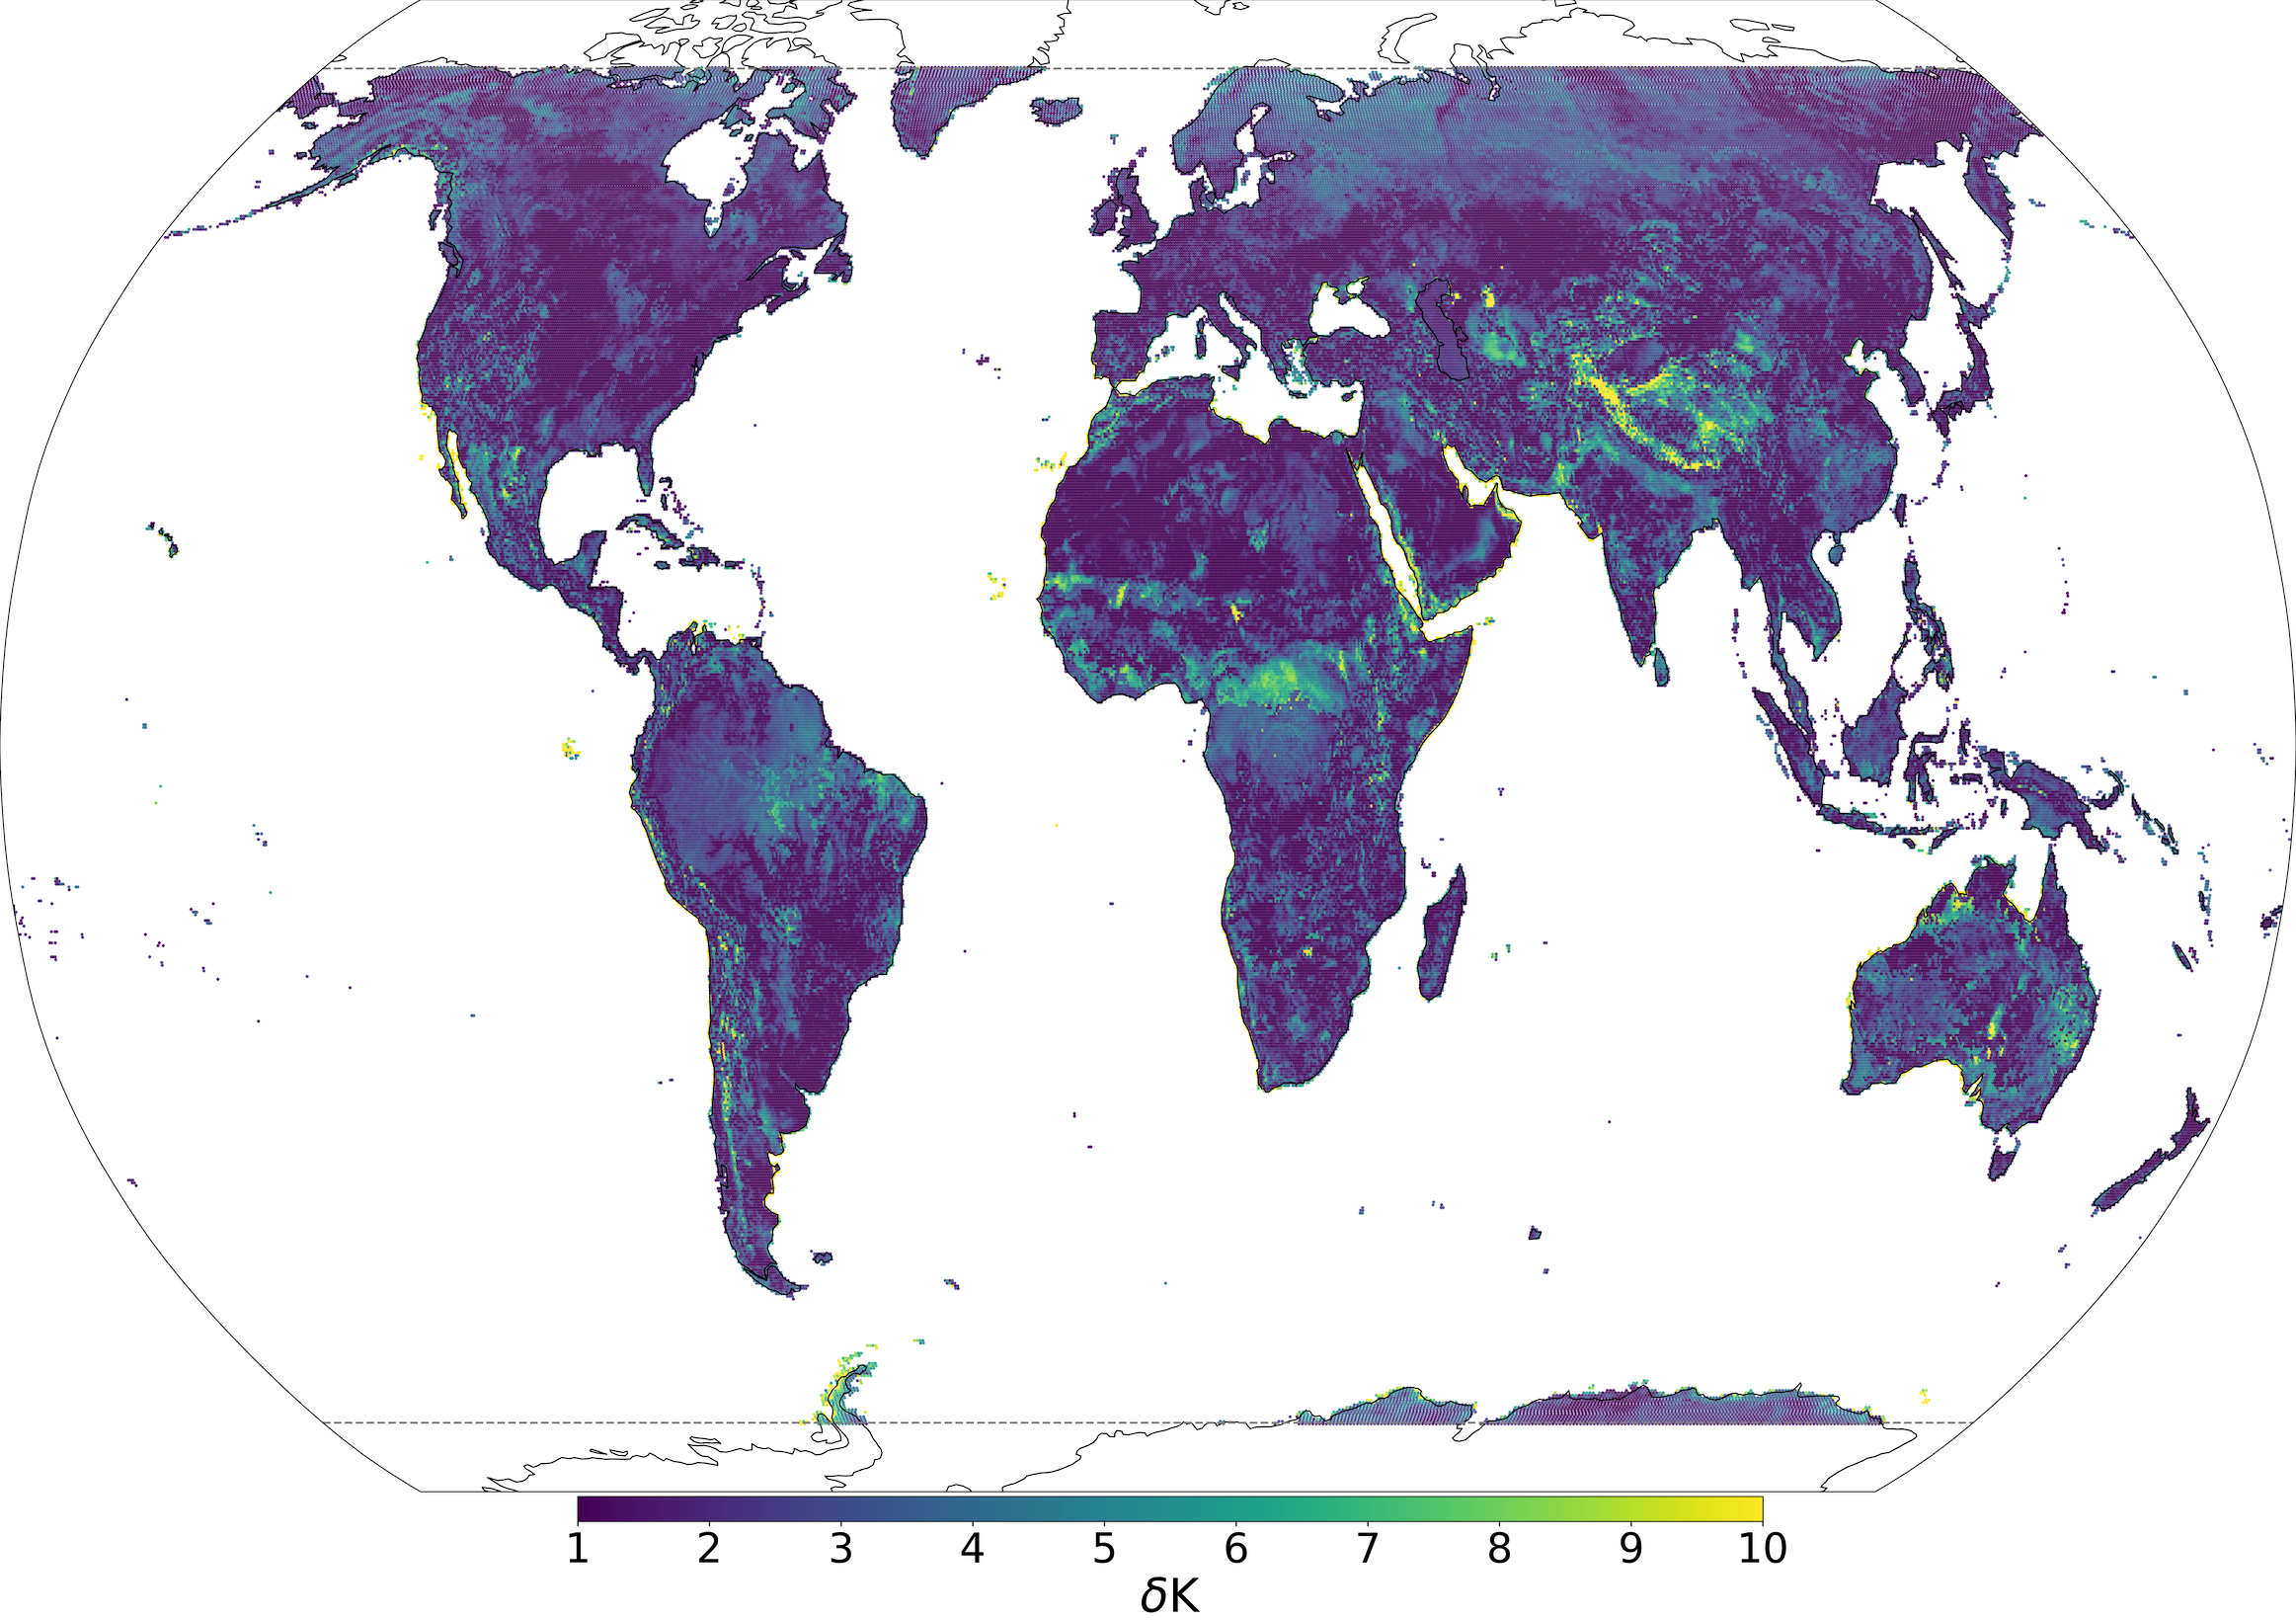
\includegraphics[width=0.48\textwidth]{ERA_prediction_error.png}} \DIFaddFL{\hspace{1mm}
 	}\subfloat[\label{fig:wasserstein_precipitation}]{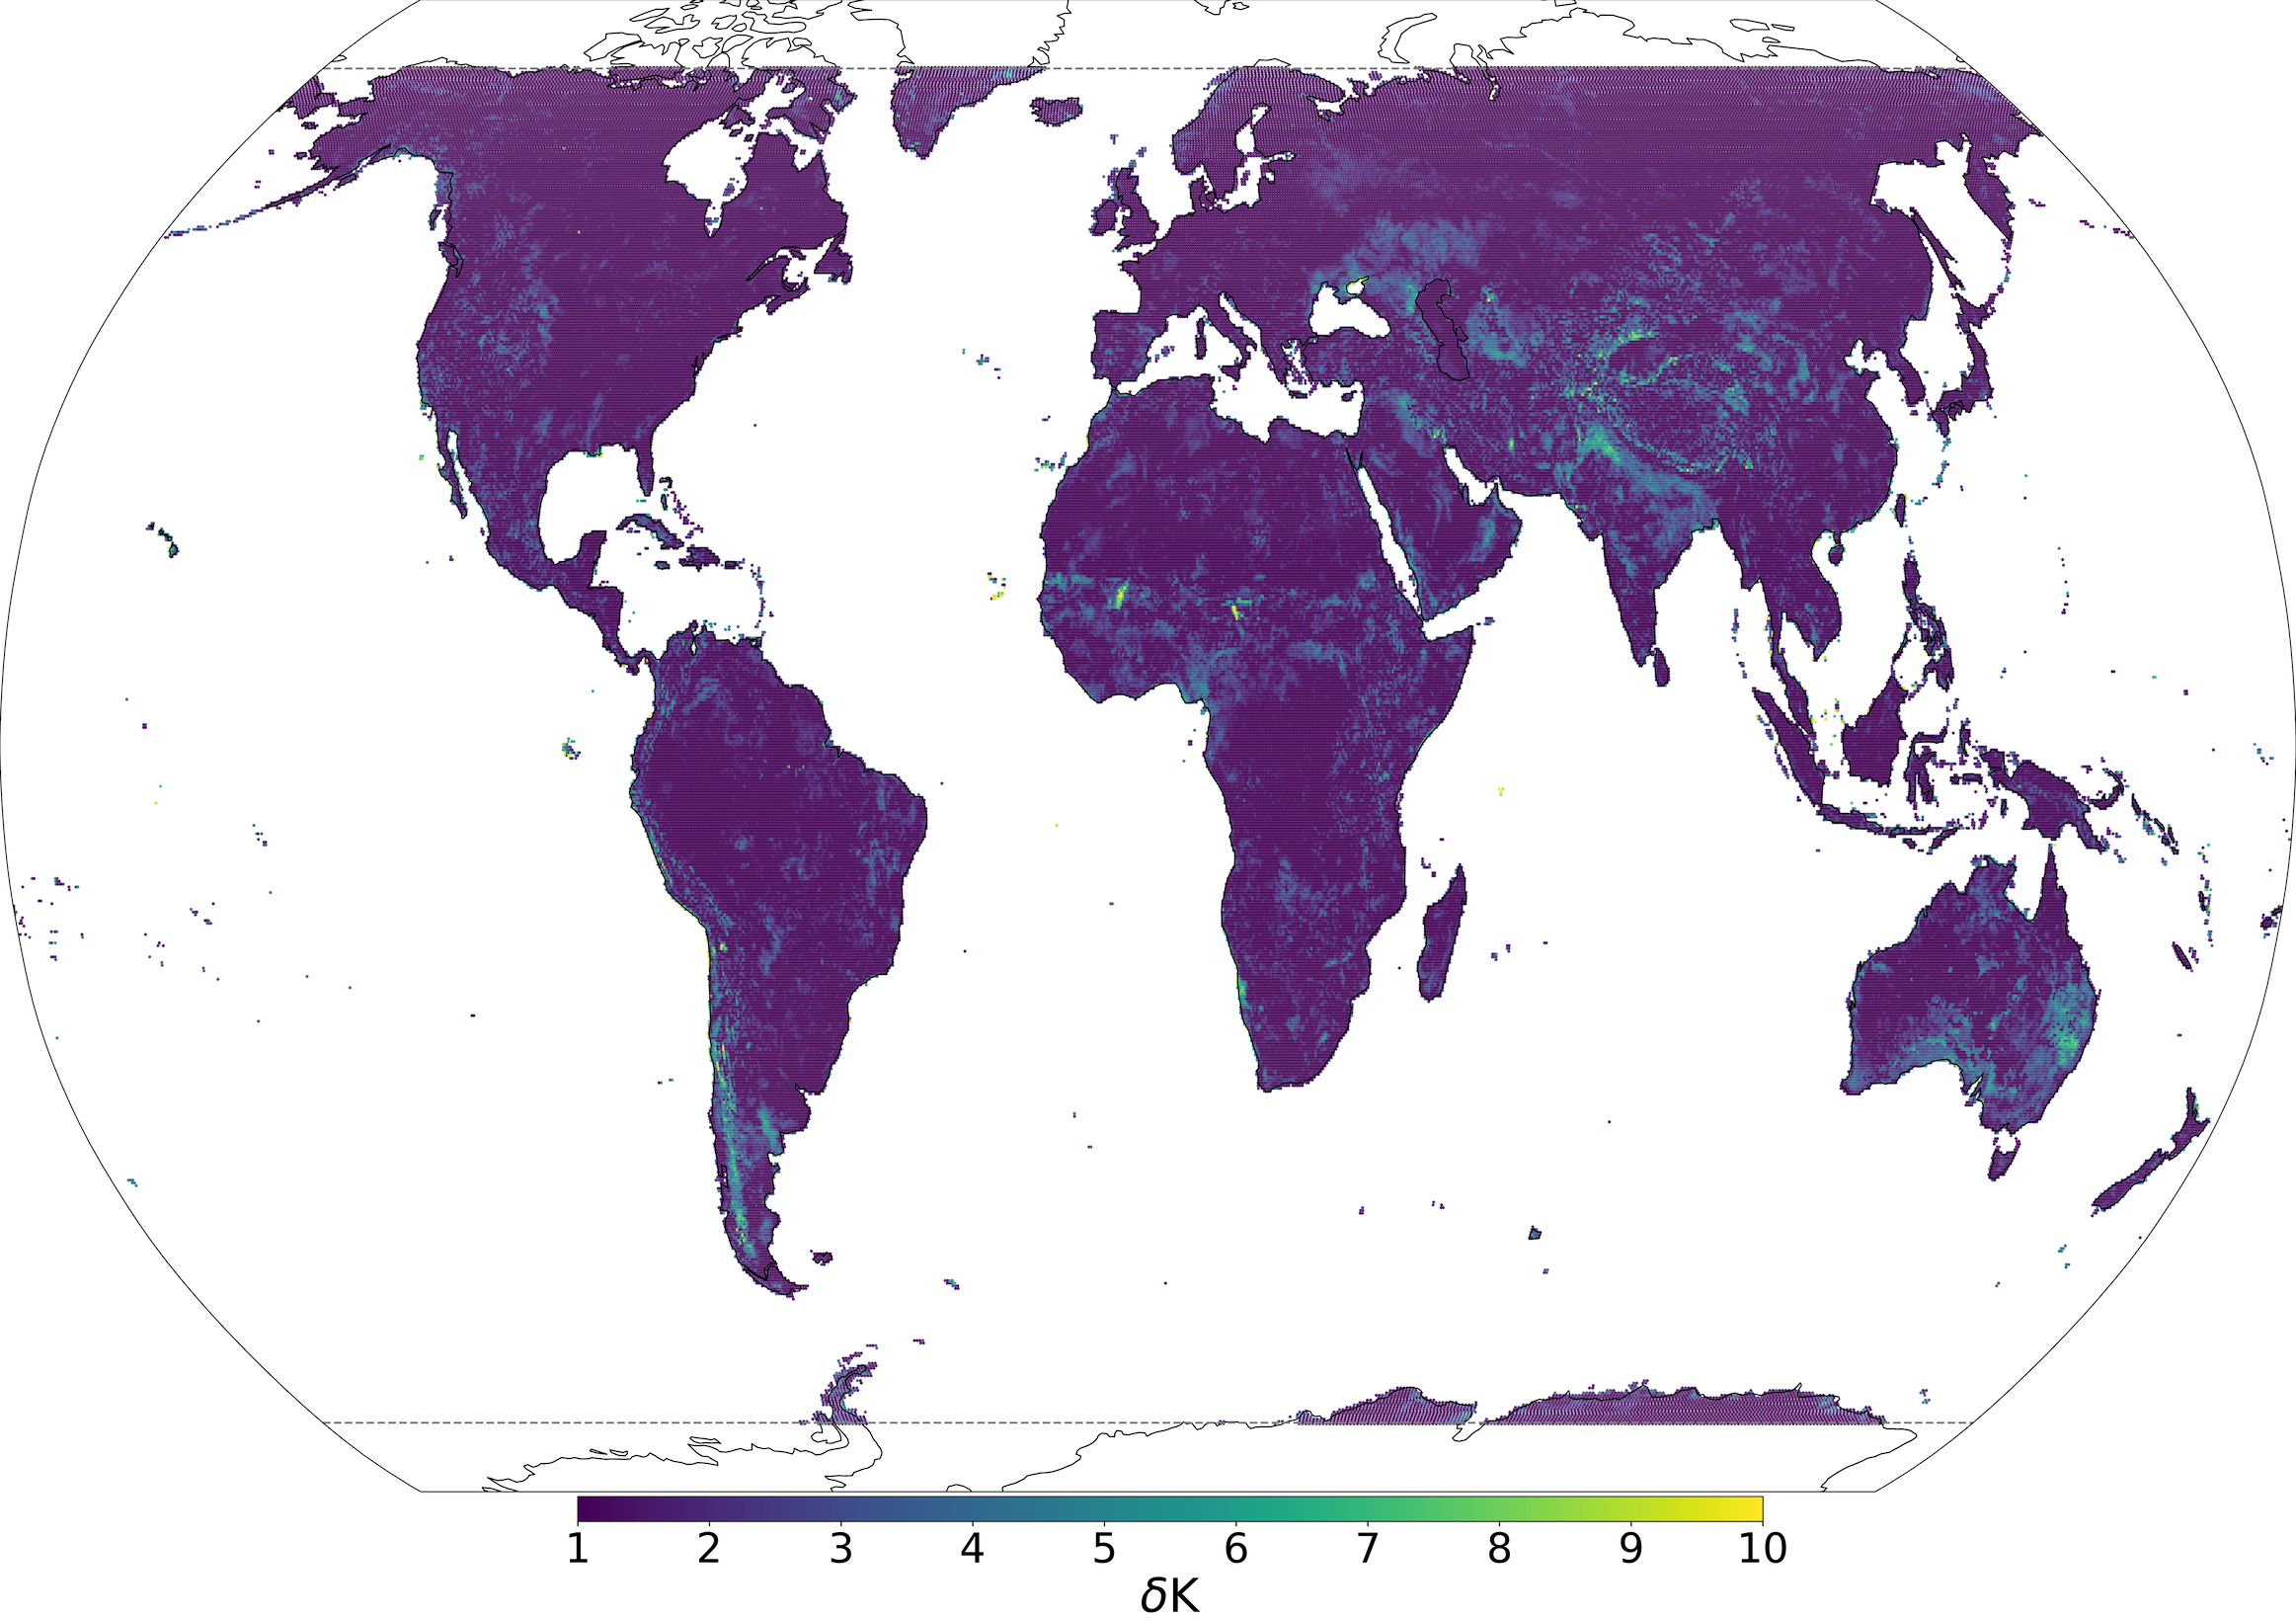
\includegraphics[width=0.48\textwidth]{model_prediction_error.png}}
 	\caption{\DIFaddFL{Mean absolute error (MAE, $\delta K$) of LST predictions for 2019 at ~31km resolution based on differences between (a) ERA5 skin temperature and Aqua-MODIS LST and  (b) between VESPER\_V15 (i.e. VESPER trained with V15 surface physiographic fields) and Aqua-MODIS LST. It can be seen that VESPER\_V15 managed to learn corrections over regions with complex surface fields such as the Himalayas (lots of orography) sub-Saharan Africa (lots of vegetation) and the Amazon Basin (lots of water + vegetation). }} 
 	\label{fig:example_model}
 \end{figure*}


\DIFaddend \noindent \DIFdelbegin \DIFdel{There is an inherent noise in the regression model due to the stochasticity of the network; training the model twice with the same architecture, inputs and parameters can find two different minima. Moreover, for the majority of the globe the lake fields have not been updated, since there are no lakes there! By inspecting the predictions at a grid point where the fields have not been updated in going from V15 to V20 we obviously don't learn anything, instead just measuring the intrinsic model noise, i.e. the different optimisation minima discovered by the model. By comparing two models with the same network structure, trained on the same data, we estimate the noise bias to be 0.04 K over all grid points. Instead we want to restrict our analysis to }\DIFdelend \DIFaddbegin \DIFadd{As the focus of this study is lake-related fields, and lakes occupy only 1.8\% of the Earth’s surface and are distributed very heterogeneously \mbox{%DIFAUXCMD
\citep{Choulga2014}}\hskip0pt%DIFAUXCMD
, analysis of the results was restricted to }\DIFaddend areas where there have been \DIFdelbegin \DIFdel{a }\DIFdelend significant changes in the \DIFdelbegin \DIFdel{fields. More quantitively, we consider a }\DIFdelend \DIFaddbegin \DIFadd{surface lake physiographic fields. By }\DIFaddend ``significant change" \DIFdelbegin \DIFdel{to be }\DIFdelend \DIFaddbegin \DIFadd{we mean }\DIFaddend a change in \DIFaddbegin \DIFadd{any of }\DIFaddend the surface field when going from V15 to V20 \DIFdelbegin \DIFdel{of $\geq 0.1 $ }\DIFdelend \DIFaddbegin \DIFadd{(and to V15X or V20X) of ≥ 10\% (≥ 0.1 }\DIFaddend for fractional fields\DIFdelbegin \DIFdel{of  $\geq 10 \%$ for non-fractional quantities. So for example , if the field for the lake cover (}\textit{\DIFdel{cl}}%DIFAUXCMD
\DIFdel{) - which describes the fraction of the grid box which is classified as a lake - changes }\DIFdelend \DIFaddbegin \DIFadd{); for example if lake or vegetation cover changed }\DIFaddend from 0.1 in V15 to 0.3 in V20 \DIFdelbegin \DIFdel{this would be classified as a significantchange. Similarly, if the lake depth - a non fractional quantity - changes from 10m to 20m, this would also be a significant change. Naturally the choice of $\geq 10 \%$ is a somewhat arbitrary tolerance }\DIFdelend \DIFaddbegin \DIFadd{field set this change is classified as significant. The choice of ≥ 10 \% as a significance }\DIFaddend cut-off \DIFdelbegin \DIFdel{, but it balances the }\DIFdelend \DIFaddbegin \DIFadd{was adopted as it proved to be a good }\DIFaddend trade off between having a sufficient number of grid points to inspect and the strength of the effect of changing the input field. As the \DIFdelbegin \DIFdel{tolerance increases we isolate points where the fields have been changed more severely, but have fewer points, }\DIFdelend \DIFaddbegin \DIFadd{cut-off \% increases less points are selected, albeit with more severe changes to their surface fields, }\DIFaddend whereas when the \DIFdelbegin \DIFdel{tolerance decreases we have more points but it is }\DIFdelend \DIFaddbegin \DIFadd{cut-off \% decreases }\DIFaddend more \DIFaddbegin \DIFadd{points are selected but it becomes more }\DIFaddend difficult to disentangle the change in the prediction accuracy from \DIFdelbegin \DIFdel{the model noise . Alternative tolerances }\DIFdelend \DIFaddbegin \DIFadd{VESPER’s training noise (training noise is discussed below). Alternative cut-off \% }\DIFaddend were briefly explored, but \DIFdelbegin \DIFdel{our conclusions are }\DIFdelend \DIFaddbegin \DIFadd{conclusions of the results remained }\DIFaddend broadly unchanged. \DIFdelbegin %DIFDELCMD < \newline 
%DIFDELCMD < 

%DIFDELCMD < \noindent %%%
\DIFdel{Grid points }\DIFdelend \DIFaddbegin \DIFadd{All grid-cells selected for the analysis }\DIFaddend can be classified according to how the surface fields are updated when going from V15 to V20 \DIFdelbegin \DIFdel{. We will examine 3 illustrative categories }\DIFdelend \DIFaddbegin \DIFadd{(note that categories represent a systematic and consistent update across multiple related fields, and do not include any restrictions on other surface fields apart the ones mentioned)}\DIFaddend : 
\begin{itemize}
	\item \textbf{Lake Updates}. The change in the lake cover \textit{cl} and lake depth \textit{dl} are significant, but the \DIFaddbegin \DIFadd{changes in }\DIFaddend ocean and glacier \DIFaddbegin \textit{\DIFadd{glm}} \DIFaddend fractions are not. This corresponds to \DIFdelbegin \DIFdel{grid boxes where inland }\DIFdelend \DIFaddbegin \DIFadd{grid-cells where }\DIFaddend lakes have been added or removed. \DIFdelbegin \DIFdel{We will also use }\DIFdelend \DIFaddbegin \DIFadd{Lake-Ground Updates is }\DIFaddend a sub-category \DIFdelbegin \textbf{\DIFdel{Lake-Ground Updates}} %DIFAUXCMD
\DIFdel{where we have the }\DIFdelend \DIFaddbegin \DIFadd{where }\DIFaddend additional constraint that the change in the high/low vegetation fractions \DIFaddbegin \textit{\DIFadd{cvh/cvl}} \DIFaddend are not significant \DIFaddbegin \DIFadd{is in place}\DIFaddend . This then corresponds to the exchange of lakes for bare ground, or vice versa.
	\item \textbf{Vegetation Updates\DIFdelbegin %DIFDELCMD < \MBLOCKRIGHTBRACE%%%
\DIFdelend .\DIFaddbegin } \DIFaddend The change in the high vegetation fraction \DIFaddbegin \textit{\DIFadd{cvh}} \DIFaddend is significant, but the change in lake cover \DIFaddbegin \textit{\DIFadd{cl}} \DIFaddend is not significant. This corresponds to \DIFdelbegin \DIFdel{grid boxes }\DIFdelend \DIFaddbegin \DIFadd{grid-cells }\DIFaddend where large features like forests and woodlands have been updated, exchanged for bare ground or low vegetation.
	\item \textbf{Glacier Updates}. The change in the glacier cover \textit{\DIFdelbegin \DIFdel{si10}\DIFdelend \DIFaddbegin \DIFadd{glm}\DIFaddend } is significant. This corresponds to any areas where the fraction of glacier ice has been updated.
\end{itemize}
\DIFdelbegin %DIFDELCMD < \noindent %%%
\DIFdel{These categories are naturally broad, and have no restrictions on all of the other features listed in Table \ref{tab:1}. For instance, changes to the orography will have important influences on temperature through e. g. wind, solar heating etc. Lake depth is similarly important, influencing how a lake freezes, thaws, mixes and its overall dynamical range. We therefore emphasise that these categories do not correspond to grid points where }\textit{\DIFdel{only}} %DIFAUXCMD
\DIFdel{the fields that define the categories have been updated, but instead represent a systematic and consistent update across multiple related fields. }%DIFDELCMD < \newline 
%DIFDELCMD < 

%DIFDELCMD < \noindent %%%
\DIFdel{We train the model over the entire globe for the year 2016 and make predictions of the land surface temperature for 2019. For each entry in the test set we can determine the prediction accuracy of both the }\DIFdelend \DIFaddbegin \DIFadd{The training of a neural network is inherently stochastic - the same model trained twice with the same data can settle in different local optima and so make different predictions. To make our conclusions robust against this training noise, each VESPER model is in turn trained 4 times. For each MODIS ground truth we then have 4 LST predictions per model. We define the training noise as the standard deviation, $\sigma$, in the VESPER predictions for the same input fields i.e. each VESPER\_VM model will have a corresponding training noise $\sigma_{\rm VM}$. To assess the changes of LST predictability due to the use of the updated surface physiographic fields instead of }\DIFaddend V15 \DIFaddbegin \DIFadd{field set (default) we compare the mean absolute error (MAE) between different VESPER models using the simple metric $\delta_{\rm VM}$:
}\begin{equation} 
	\DIFadd{\delta_{\rm VM} = \text{MAE}_{\rm VESPER\_VM} - \text{MAE}_{\rm VESPER\_V15} 
}\end{equation}
\DIFadd{where VM represents one of the field set versions V20, V20X or V15X, and $\text{MAE}$ is computed over the whole prediction period of 2019. In turn, the MAE is the error between the prediction of a VESPER model }\DIFaddend and \DIFdelbegin \DIFdel{V20 models . We will use a simple metric $\delta_{\rm M}$ to quantify the difference between an updated model $M$ and the baseline V15 model }\DIFdelend \DIFaddbegin \DIFadd{the Aqua-MODIS LST, }\DIFaddend i.e.
\DIFdelbegin \begin{eqnarray*}
	\DIFdel{\delta_{\rm M} = M \text{ prediction error} - \text{V15 prediction error} \ .
}\end{eqnarray*}%DIFAUXCMD
\DIFdelend \DIFaddbegin \begin{equation} 
	\DIFadd{\text{MAE}_{\rm VESPER\_VM}  = \frac{1}{N} \sum_{i=1}^{N}| \text{LST}_{i, \rm VESPER\_VM} -\text{LST}_{i, \rm MODIS} |
}\end{equation}\DIFaddend 
\DIFdelbegin \DIFdel{So for example, $\delta_{\rm V20}$ describes the gain of the V20 model relative to the V15 model}\DIFdelend \DIFaddbegin \DIFadd{for total number of predictions $N$, within a given grid-cell classification}\DIFaddend . A negative \DIFdelbegin \DIFdel{$\delta_{\rm V20}$ therefore }\DIFdelend \DIFaddbegin \DIFadd{$\delta_{\rm VM}$ then }\DIFaddend indicates that the \DIFdelbegin \DIFdel{V20 }\DIFdelend \DIFaddbegin \DIFadd{VESPER\_VM LST }\DIFaddend prediction is more accurate \DIFaddbegin \DIFadd{than the  VESPER\_V15 prediction}\DIFaddend , and vice versa.

%
%\DIFdelbegin \DIFdel{The results for the selected grid point categories are presented in Table \ref{tab:V1520_results}. }\DIFdelend \DIFaddbegin 



\section{\DIFadd{Results}}\label{sec:3}

\subsection{\DIFadd{Evaluation of updated lake fields}}
\DIFadd{To understand if there is a way to automatically and rapidly assess the accuracy of updated and/or new surface physiography fields, and if their use in the atmospheric model increase predictability, we can compare the prediction accuracy of different VESPER\_VM models. Generally VESPER’s training noise is confirmed to be smaller than differences in LST predictions by different VESPER configurations, so changes in LST predictability can be meaningfully attributed to the changes in surface physiographic fields. Particular situations where the training noise becomes significant are discussed below. }\DIFaddend \newline 

\DIFdelbegin %DIFDELCMD < \begin{table*}[t]
%DIFDELCMD < 	\centering
%DIFDELCMD < 	\begin{tabular}{llll}
%DIFDELCMD < 		%%%
\DIFdelFL{Category     }\DIFdelendFL \DIFaddbeginFL \noindent \DIFaddFL{As a first attempt lake-related information is assessed, namely lake cover (and land-sea mask and glacier cover as they are used for lake cover generation) and lake mean depth, that were created from scratch using new up-to-date high-resolution input datasets (see Table \ref{tab:datasources}) for the V20 (and V20X) field set; other surface physiographic fields (see Table \ref{table:definitions}) were regenerated from the same input sources as in the initial V15 field set, but taking into account that lake related fields were changed. In cases when existing in V15 lake cover water was removed in V20, it could be replaced by any of high or low vegetation, glacier or bare ground. We now analyse the results for each of the 4 categories of grid cell in detail (see Table \ref{tab:categorisation} for the results of each category aggregated over the whole globe).
	
	
	
	
	
	
	
	
	
	
%}\begin{table*}
%	\begin{tabular}{ccccccccc}
%		\toprule
%		\multirow{2}{*}{Category} \DIFaddendFL & \DIFdelbeginFL \DIFdelFL{Number of grid points         }\DIFdelendFL \DIFaddbeginFL \multirow{2}{*}{Number of grid cells} \DIFaddendFL & 	\DIFdelbeginFL \DIFdelFL{Mean $\delta_{\rm V20}$ (K)}\DIFdelendFL \DIFaddbeginFL \multicolumn{4}{c}{$\sigma_{\rm VM}$, $K$} \DIFaddendFL &\DIFdelbeginFL \DIFdelFL{Mean $\delta_{\rm V20X}$ (K)}\DIFdelendFL \DIFaddbeginFL \multicolumn{3}{c}{$\delta_{\rm VM}$, $K$} \DIFaddendFL \\  
%		\DIFaddbeginFL &&\DIFaddFL{V15  }& \DIFaddFL{V15X }& \DIFaddFL{V20 }& \DIFaddFL{V20X }& \DIFaddFL{V15X }&\DIFaddFL{V20 }& \DIFaddFL{V20X  }\\
%		\DIFaddendFL \hline 
%		Lake&1631 & \DIFdelbeginFL \DIFdelFL{-0.450 }\DIFdelendFL \DIFaddbeginFL \DIFaddFL{0.07}\DIFaddendFL & \DIFdelbeginFL \DIFdelFL{-0.451}\DIFdelendFL \DIFaddbeginFL \DIFaddFL{0.02}& \DIFaddFL{0.02}& \DIFaddFL{0.02}&  \DIFaddFL{-0.20 }& \DIFaddFL{-0.37}&\DIFaddFL{-0.37 }\DIFaddendFL \\
%		Lake-Ground&546 & \DIFdelbeginFL \DIFdelFL{-1.12}\DIFdelendFL \DIFaddbeginFL \DIFaddFL{0.15 }\DIFaddendFL &\DIFdelbeginFL \DIFdelFL{-1.09 }\DIFdelendFL \DIFaddbeginFL \DIFaddFL{0.05}& \DIFaddFL{0.04}& \DIFaddFL{0.06 }& \DIFaddFL{-0.56 }&\DIFaddFL{-0.83}& \DIFaddFL{-0.84 }\DIFaddendFL \\
%		Vegetation&58 & \DIFdelbeginFL \DIFdelFL{+0.49 }\DIFdelendFL \DIFaddbeginFL \DIFaddFL{0.04 }\DIFaddendFL &\DIFdelbeginFL \DIFdelFL{+0.0048}\DIFdelendFL \DIFaddbeginFL \DIFaddFL{0.10}& \DIFaddFL{0.15}& \DIFaddFL{0.21}&  \DIFaddFL{-0.00}&\DIFaddFL{0.04 }& \DIFaddFL{-0.00 }\DIFaddendFL \\
%		Glacier&1057 & \DIFdelbeginFL \DIFdelFL{-0.14 }\DIFdelendFL \DIFaddbeginFL \DIFaddFL{0.03}\DIFaddendFL & \DIFdelbeginFL \DIFdelFL{-0.24}\DIFdelendFL \DIFaddbeginFL \DIFaddFL{0.08}& \DIFaddFL{0.02}& \DIFaddFL{0.06 }& \DIFaddFL{-0.01}& \DIFaddFL{-0.22}& \DIFaddFL{-0.28  }\DIFaddendFL \\
%		\DIFdelbeginFL %DIFDELCMD < \hline
%%DIFDELCMD < 	%%%
%\DIFdelendFL \DIFaddbeginFL \bottomrule
%	\DIFaddendFL \end{tabular}
%	\caption{\DIFdelbeginFL \DIFdelFL{Mean change in the model prediction accuracy when using the updated fields,  for the selected update categories. The }\DIFdelendFL \DIFaddbeginFL \DIFaddFL{Globally averaged differences $\delta_{\rm VM}$ between }\DIFaddendFL mean \DIFdelbeginFL \DIFdelFL{$\delta_{\rm M}$ }\DIFdelendFL \DIFaddbeginFL \DIFaddFL{absolute error (MAE) of VESPER\_VM  and VESPER\_V15 LST for 2019 at ~31km resolution (where M }\DIFaddendFL denotes \DIFdelbeginFL \DIFdelFL{the annual average over all grid points within a }\DIFdelendFL \DIFaddbeginFL \DIFaddFL{V15X, V20, V20X field sets) per grid-cell }\DIFaddendFL category. Negative \DIFdelbeginFL \DIFdelFL{$\delta_{\rm M}$ }\DIFdelendFL \DIFaddbeginFL \DIFaddFL{$\delta_{\rm VM}$ }\DIFaddendFL values indicate \DIFdelbeginFL \DIFdelFL{that }\DIFdelendFL \DIFaddbeginFL \DIFaddFL{an increase of LST predictability due to }\DIFaddendFL the \DIFdelbeginFL \DIFdelFL{addition }\DIFdelendFL \DIFaddbeginFL \DIFaddFL{use }\DIFaddendFL of the updated \DIFaddbeginFL \DIFaddFL{surface physiographic }\DIFaddendFL fields \DIFdelbeginFL \DIFdelFL{has improved the prediction}\DIFdelendFL \DIFaddbeginFL \DIFaddFL{instead of V15 field set (default)}\DIFaddendFL , \DIFdelbeginFL \DIFdelFL{whilst }\DIFdelendFL positive \DIFdelbeginFL \DIFdelFL{$\delta_{\rm M}$ }\DIFdelendFL \DIFaddbeginFL \DIFaddFL{$\delta_{\rm VM}$ }\DIFaddendFL values indicate \DIFdelbeginFL \DIFdelFL{that }\DIFdelendFL \DIFaddbeginFL \DIFaddFL{a decrease in }\DIFaddendFL the \DIFdelbeginFL \DIFdelFL{prediction accuracy has degraded, suggesting that }\DIFdelendFL \DIFaddbeginFL \DIFaddFL{LST predictability and suggests the presence of }\DIFaddendFL erroneous information \DIFdelbeginFL \DIFdelFL{has been introduced}\DIFdelendFL \DIFaddbeginFL \DIFaddFL{in the surface physiographic fields}\DIFaddendFL . \DIFaddbeginFL \DIFaddFL{Training noise values, $\sigma_{\rm VM}$, are generally much smaller than the variance between different VESPER configurations, indicating that changes in LST predictability are mainly due to changes in the surface physiographic fields. The quoted noise is the standard deviation of the prediction errors of Fig. \ref{fig:global_shift_plot}.}\DIFaddendFL }
%	\DIFdelbeginFL %DIFDELCMD < \label{tab:V1520_results}
%%DIFDELCMD < %%%
%\DIFdelendFL \DIFaddbeginFL \label{tab:categorisation}
%\DIFaddendFL \end{table*}	
%\DIFaddbegin \begin{figure}
%	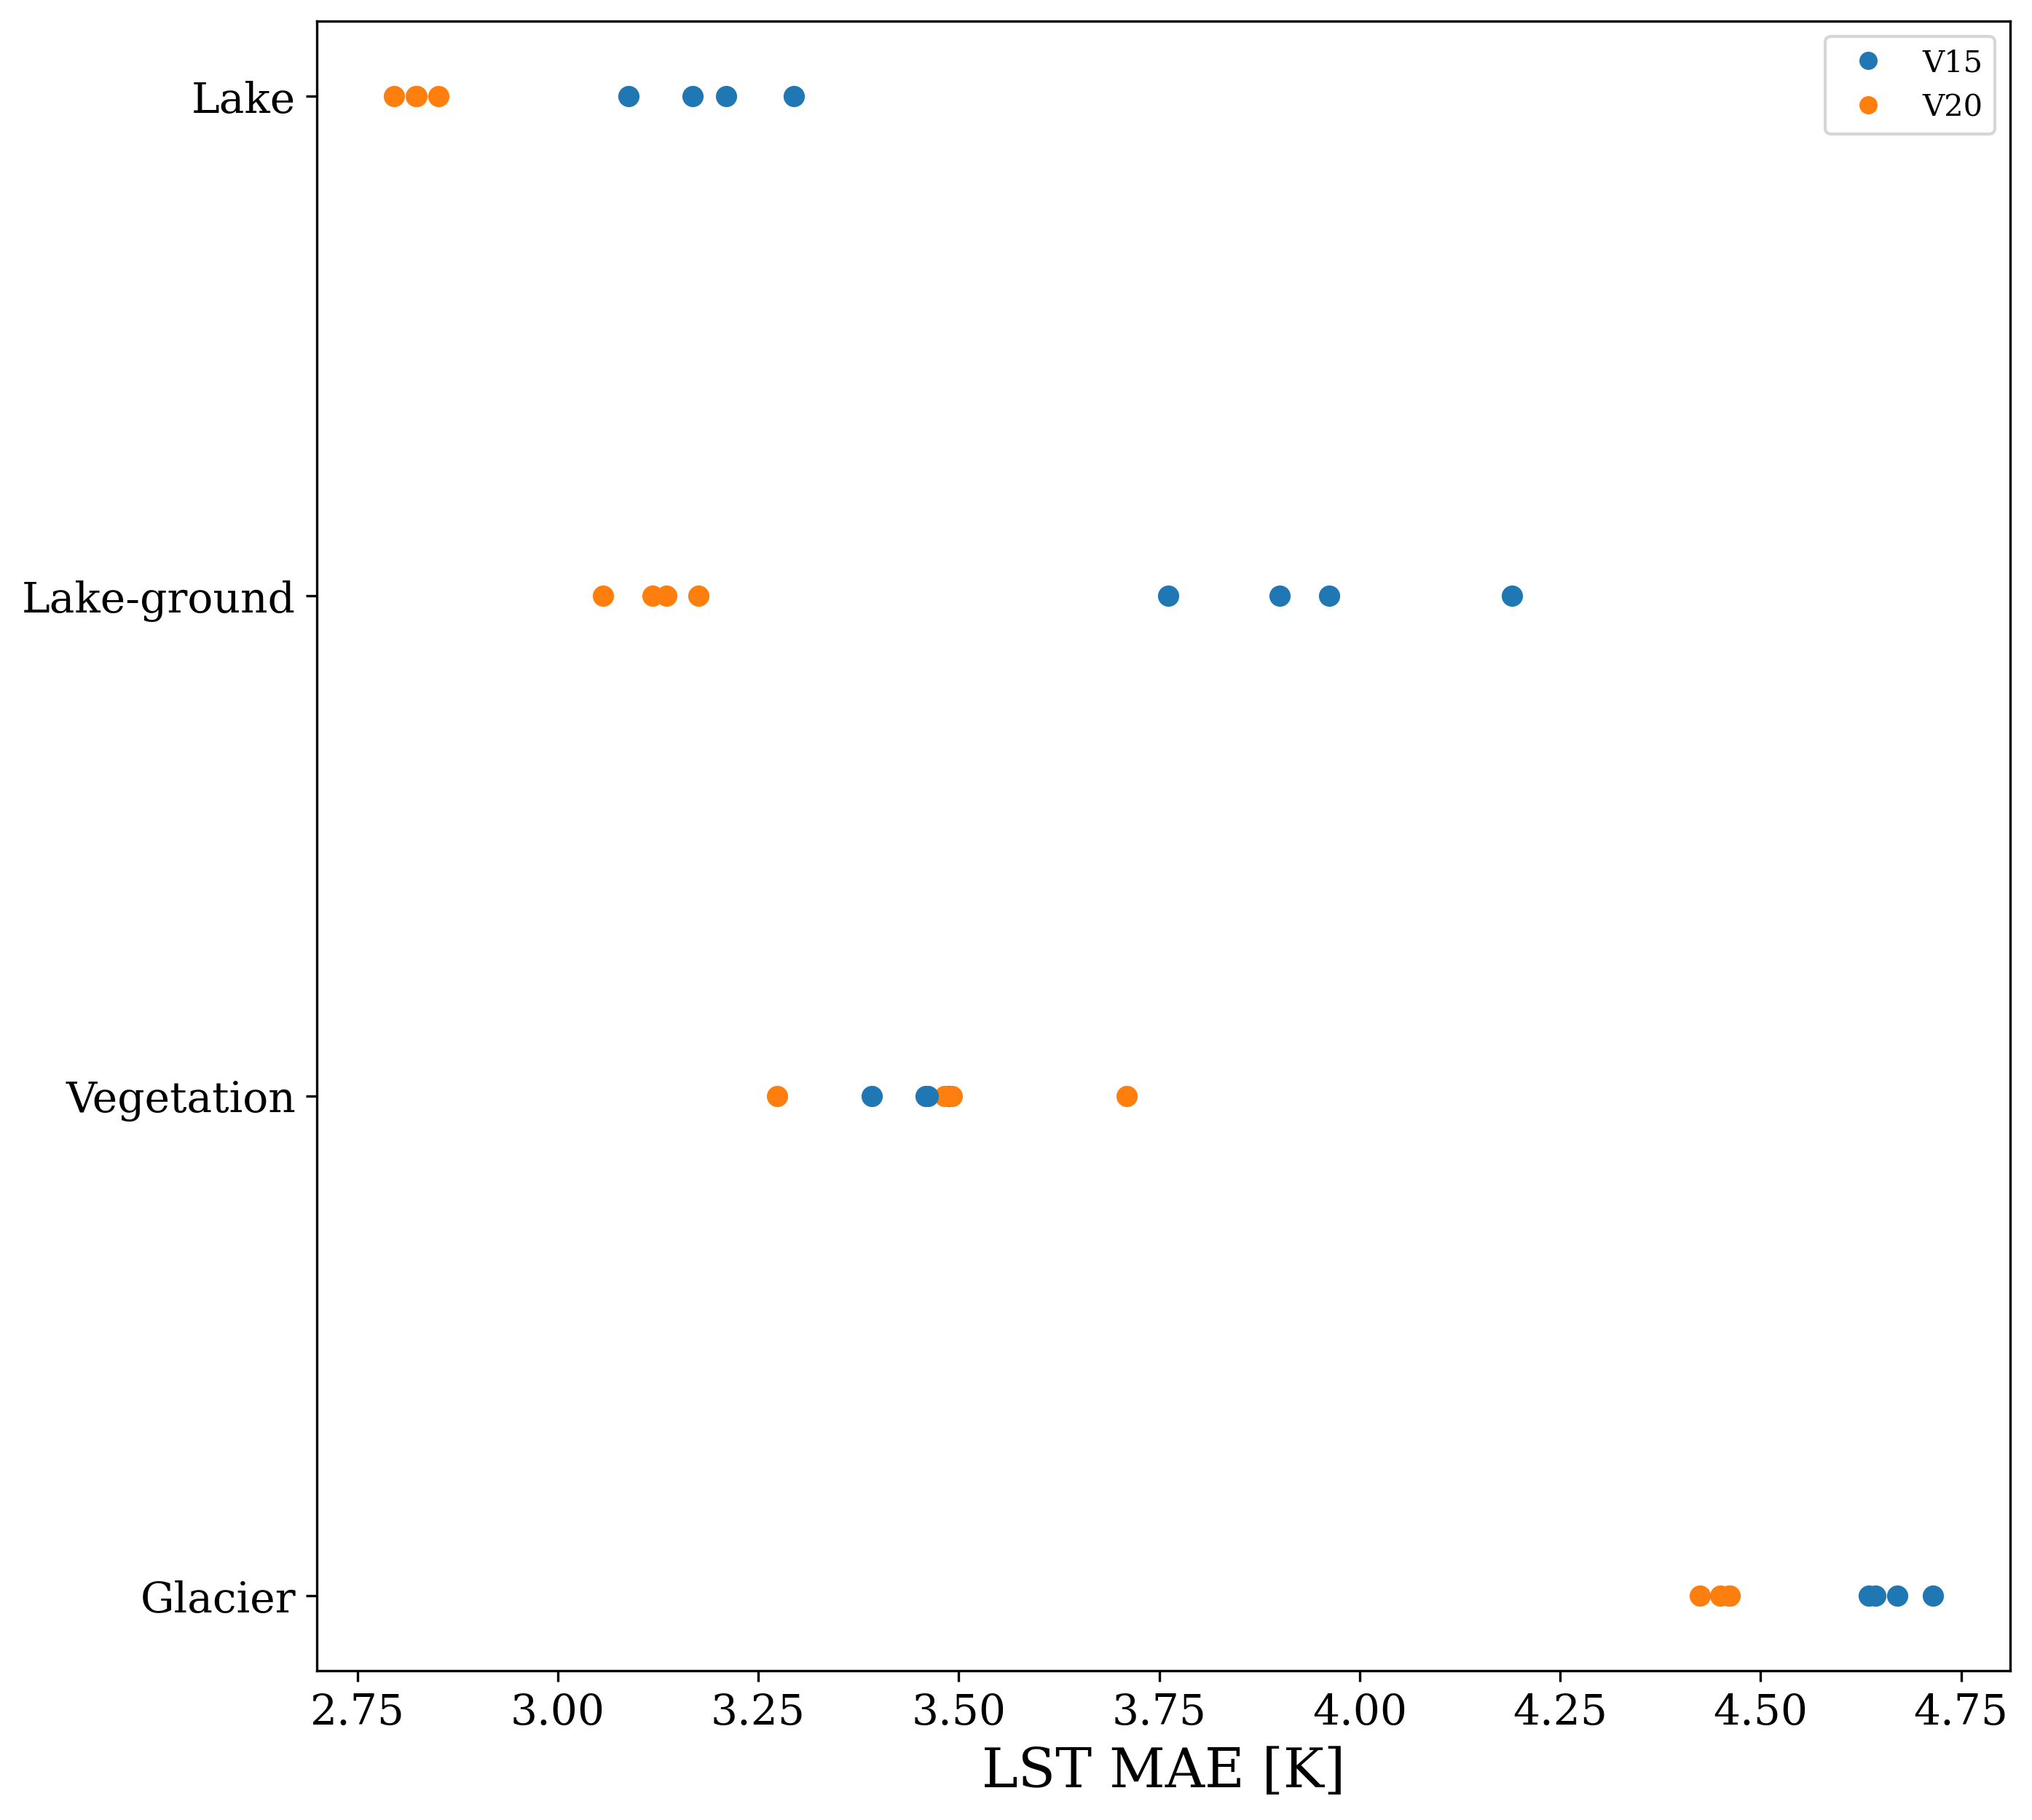
\includegraphics[width=\columnwidth]{global_shift_plot}
%	\caption{\DIFaddFL{Distribution of prediction errors in the LST, for each of the 4 grid point categories, for each iteration of V15 and V20. For Lake, Lake-ground and Glacier categories the improvement in V20 relative to V15 is much greater than the intrinsic model noise, with all V20 predictions outperforming all V15 predictions. For the Vegetation category the predictions of V15 and V20 are much more noisy and it is difficult to draw any conclusions for the category as a whole.}} 
%	\label{fig:global_shift_plot}
%\end{figure}

\DIFaddend 


\subsubsection{Category: Lake \DIFdelbegin \DIFdel{Updates}\DIFdelend \DIFaddbegin \DIFadd{updates}\DIFaddend }\DIFdelbegin %DIFDELCMD < \label{V20Lake}
%DIFDELCMD < \begin{figure*}[t]
%DIFDELCMD < 	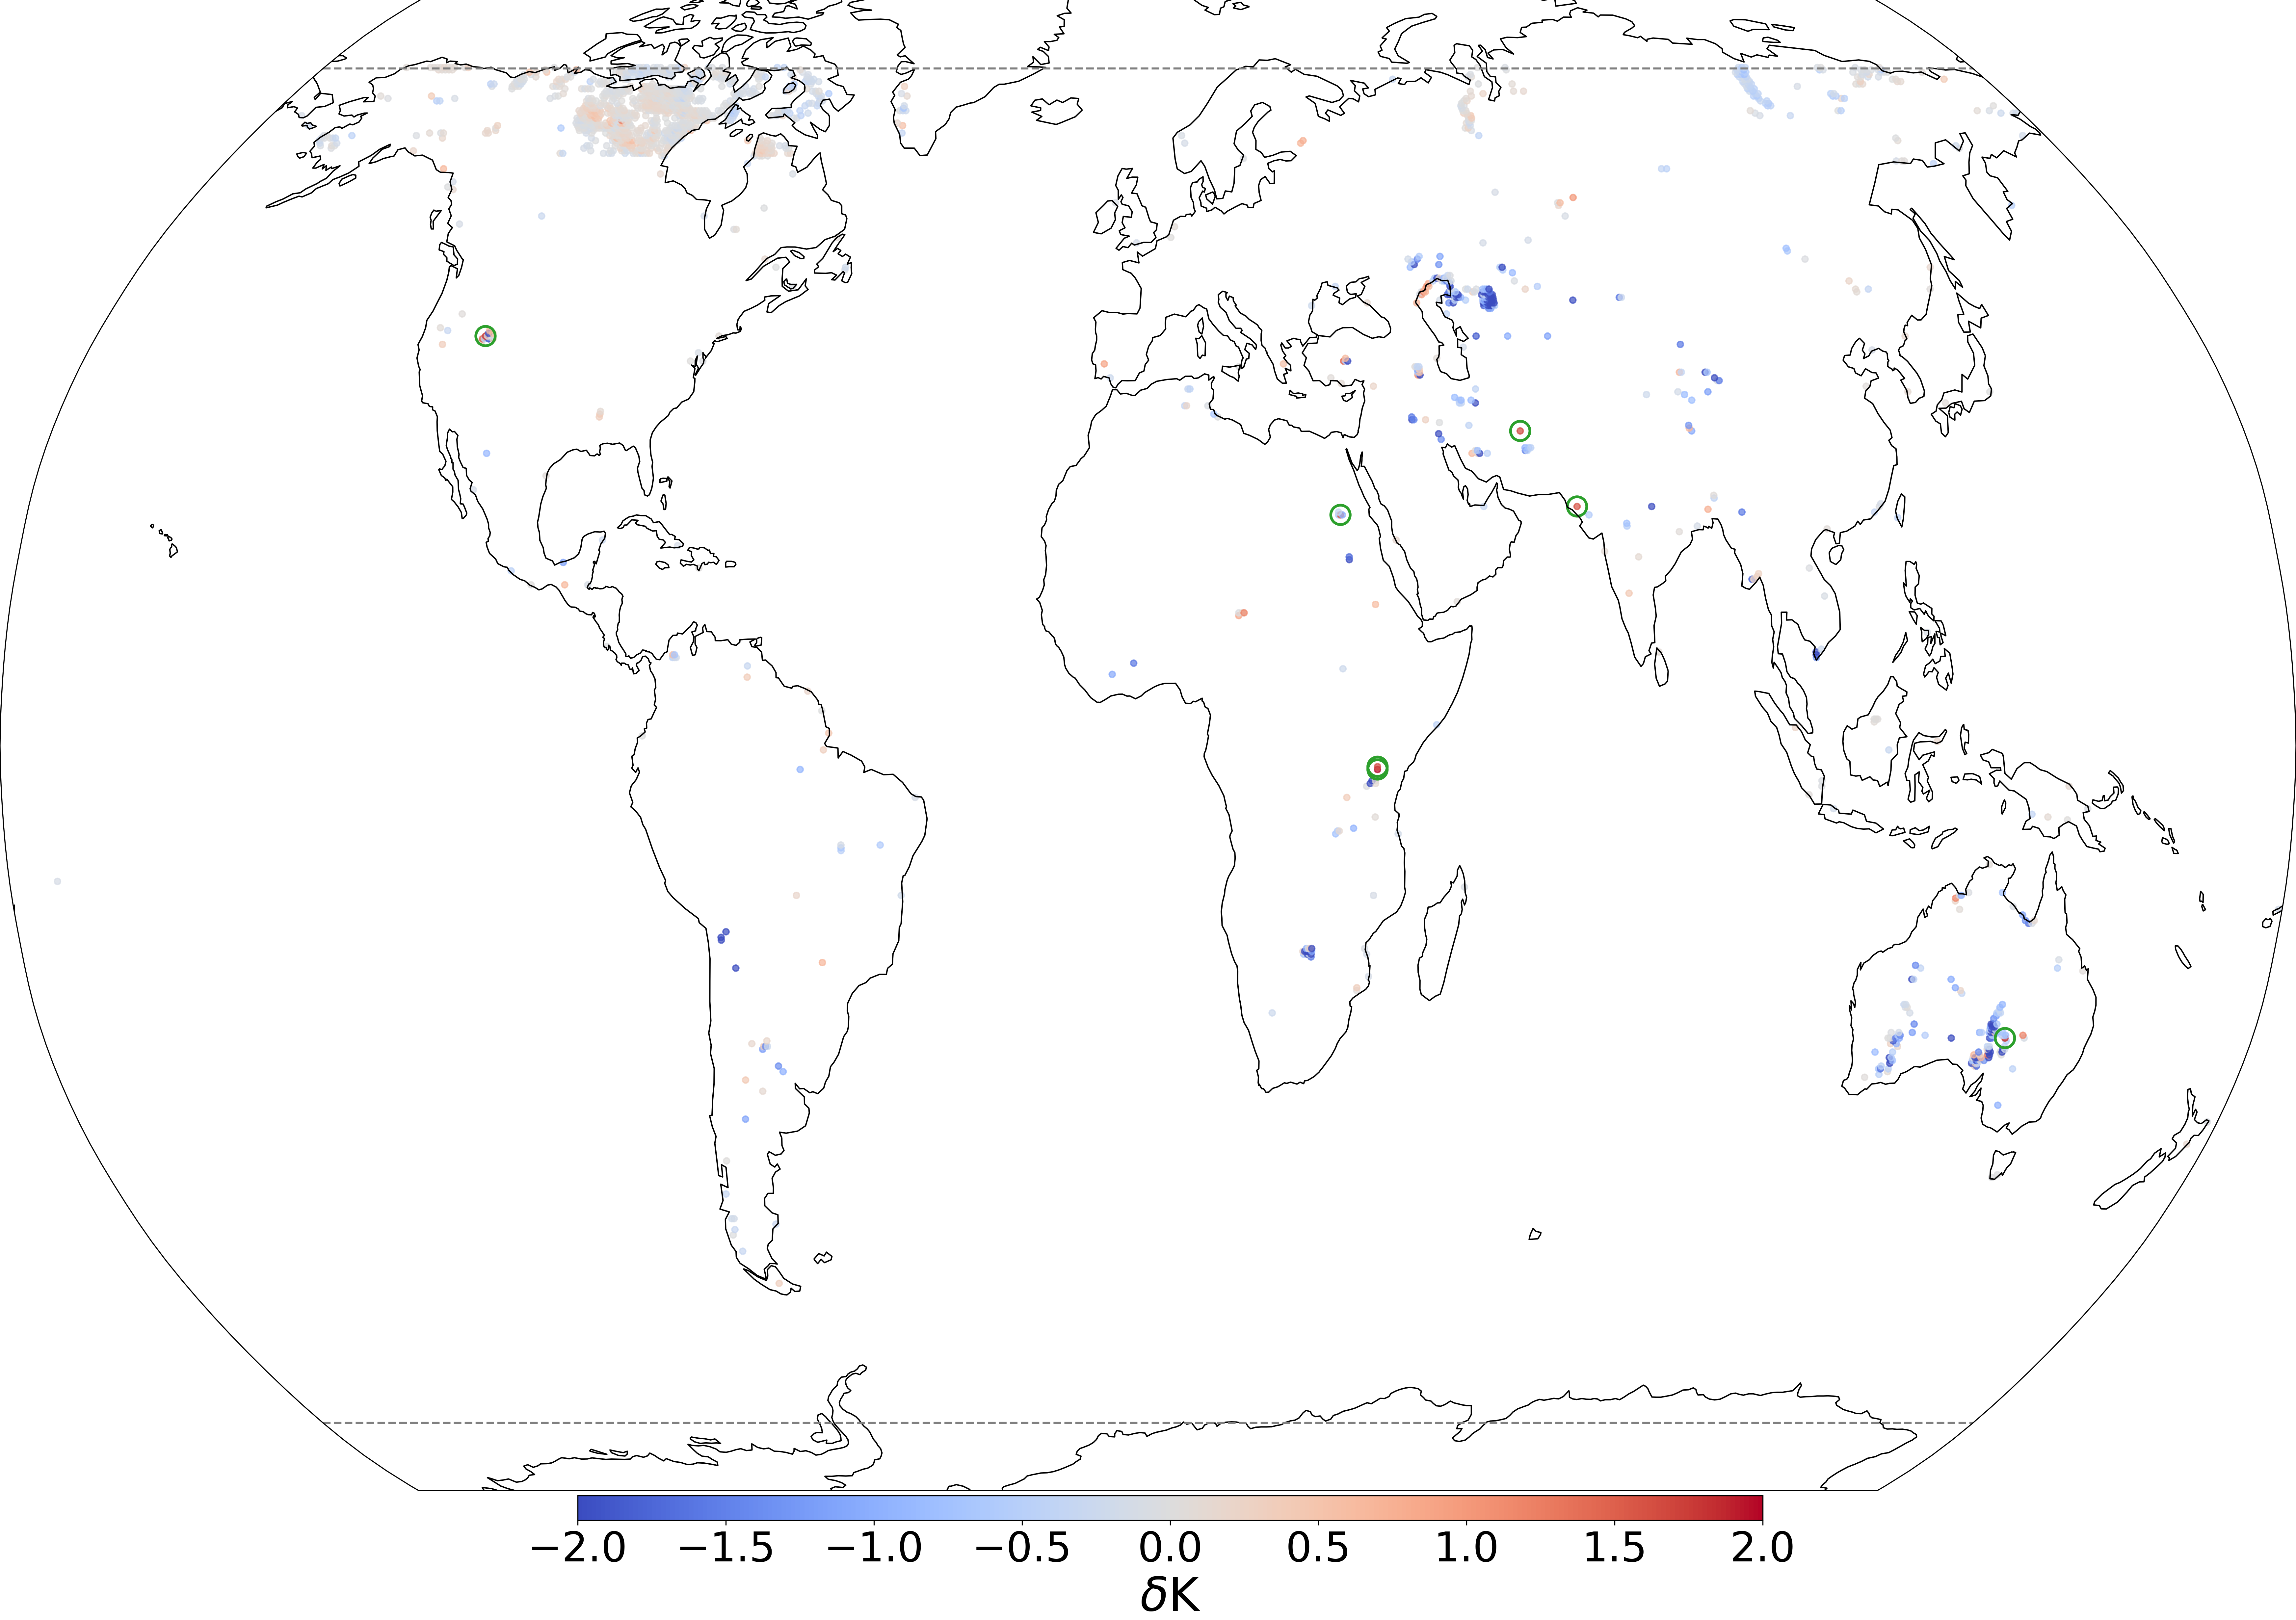
\includegraphics[width=0.98\textwidth]{lake_haver.png}
%DIFDELCMD < 	%%%
\DIFdelendFL \DIFaddbeginFL \label{sec:lake1}
\begin{figure}
	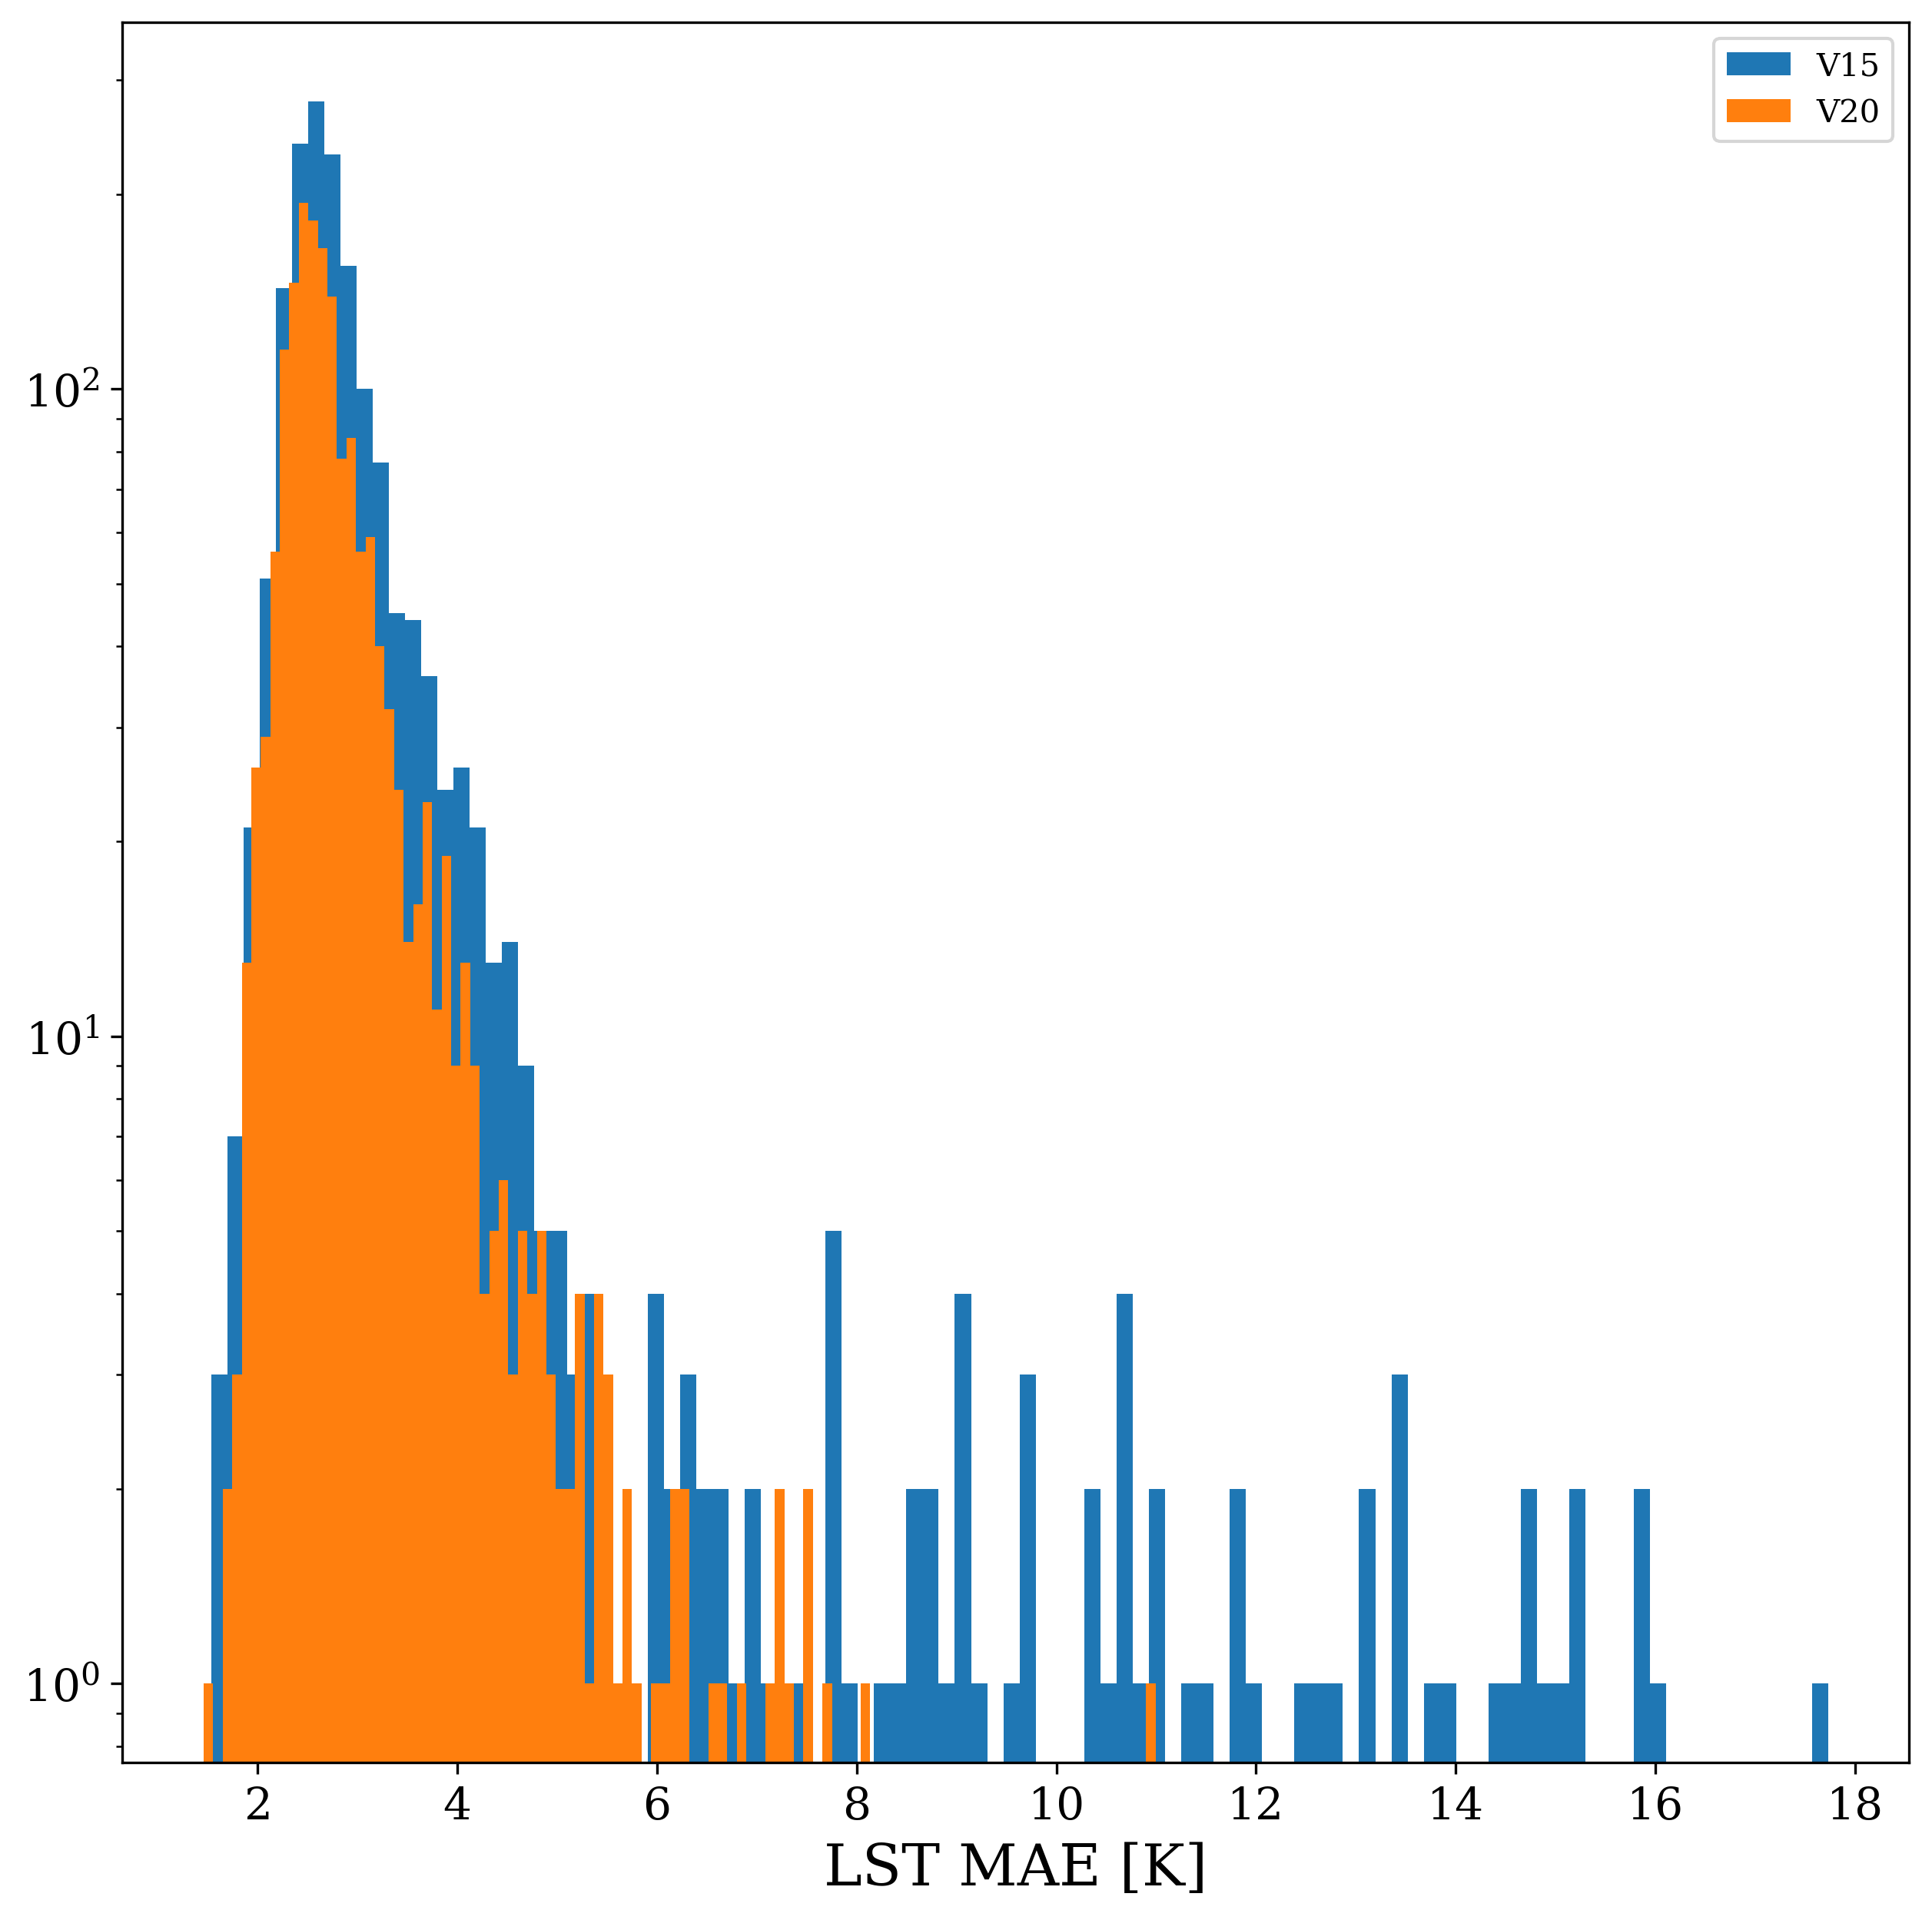
\includegraphics[width=\columnwidth]{lakes_histogram_plot}
	\DIFaddendFL \caption{\DIFdelbeginFL \DIFdelFL{Mean $\delta$ for }\DIFdelendFL \DIFaddbeginFL \DIFaddFL{Distribution of prediction errors in }\DIFaddendFL the \DIFdelbeginFL \DIFdelFL{V20 model relative to the V15 model across the globe }\DIFdelendFL \DIFaddbeginFL \DIFaddFL{LST }\DIFaddendFL for \DIFaddbeginFL \DIFaddFL{all }\DIFaddendFL grid points \DIFdelbeginFL \DIFdelFL{where all }\DIFdelendFL \DIFaddbeginFL \DIFaddFL{in }\DIFaddendFL the \DIFdelbeginFL \DIFdelFL{lake fields have changed significantly (``}\DIFdelendFL Lake \DIFdelbeginFL \DIFdelFL{Update'' }\DIFdelendFL \DIFaddbeginFL \DIFaddFL{Updates }\DIFaddendFL category \DIFdelbeginFL \DIFdelFL{)}\DIFdelendFL \DIFaddbeginFL \DIFaddFL{for VESPER\_V15 and VESPER\_V20}\DIFaddendFL .  \DIFdelbeginFL \DIFdelFL{Generally }\DIFdelendFL \DIFaddbeginFL \DIFaddFL{Each prediction errors is in turn }\DIFaddendFL the \DIFdelbeginFL \DIFdelFL{updated V20 fields enable }\DIFdelendFL \DIFaddbeginFL \DIFaddFL{average of 4 trained iterations of }\DIFaddendFL the \DIFaddbeginFL \DIFaddFL{VESPER }\DIFaddendFL model\DIFdelbeginFL \DIFdelFL{to make more accurate }\DIFdelendFL \DIFaddbeginFL \DIFaddFL{. The }\DIFaddendFL predictions \DIFdelbeginFL \DIFdelFL{, for example in the Aral sea and Australia, indicating that these updated fields }\DIFdelendFL \DIFaddbeginFL \DIFaddFL{of VESPER\_V20 }\DIFaddendFL are \DIFdelbeginFL \DIFdelFL{informative }\DIFdelendFL \DIFaddbeginFL \DIFaddFL{evidently }\DIFaddendFL and \DIFdelbeginFL \DIFdelFL{accurate. In contrast}\DIFdelendFL \DIFaddbeginFL \DIFaddFL{improvement over VESPER\_V15}\DIFaddendFL , \DIFdelbeginFL \DIFdelFL{there are some regions where the predictions get worse,  }\DIFdelendFL \DIFaddbeginFL \DIFaddFL{especially }\DIFaddendFL for \DIFdelbeginFL \DIFdelFL{example at higher latitudes which is likely due to these being regions where lakes have more complex, time variable behaviour (e.g. freezing/thawing) and MODIS satellite data is sparse e.g. due to clouds. 7 }\DIFdelendFL \DIFaddbeginFL \DIFaddFL{grid }\DIFaddendFL points \DIFdelbeginFL \DIFdelFL{(two are overlaid in sub-Saharan Africa) where the V20 prediction gets notably worse than V15 are highlighted }\DIFdelendFL with \DIFdelbeginFL \DIFdelFL{green circles and discussed in the text}\DIFdelendFL \DIFaddbeginFL \DIFaddFL{large LST errors}\DIFaddendFL .} 
	\DIFdelbeginFL %DIFDELCMD < \label{fig:bitstring_100110}
%DIFDELCMD < \end{figure*}
%DIFDELCMD < \noindent %%%
\DIFdel{The first category where we see significant improvements is for the }\DIFdelend \DIFaddbegin \label{fig:example_figure_histogram}
\end{figure}
\DIFadd{The }\DIFaddend Lake Updates category \DIFdelbegin \DIFdel{. These points are presented in Figure \ref{fig:bitstring_100110}.  We can see that there have been significant improvements globally (the mean improvement in the prediction accuracy when using the }\DIFdelend \DIFaddbegin \DIFadd{shows significant improvements in LST predictability if using }\DIFaddend V20 \DIFdelbegin \DIFdel{fields was 0.45 K, over }\DIFdelend \DIFaddbegin \DIFadd{field set instead of V15 – prediction accuracy increased globally (over }\DIFaddend 1631 \DIFdelbegin \DIFdel{grid points), most notably in Australia and the Aral sea. These were two of the major regions that we discussed earlier where in }\DIFdelend \DIFaddbegin \DIFadd{grid-cells) on average by 0.37K. For the lakes category, the training noise in }\DIFaddend V20 \DIFdelbegin \DIFdel{we have removed the ephemeral water (e.g. for Australia) and corrected lake sizes (e.g. for the Aral sea). By providing this updated information to the model that there is less water than initially thought in these regions, the model can then make more accurate predictions. This is a clear example of a verification of the updated fields }\DIFdelend \DIFaddbegin \DIFadd{was generally small $\sigma_{\rm V20} \sim 0.02$ K, with the V15 predictions a little more noisy with $\sigma_{\rm V15} \sim 0.07$ K, but this noise is much less than the improvement }\DIFaddend - \DIFdelbegin \DIFdel{it gives us confidence that these new fields are indeed more accurate and are also informative (i.e.predictive)with respect to surface temperatures. }\DIFdelend \DIFaddbegin \DIFadd{as can be seen in Fig. \ref{fig:global_shift_plot} every V20 iteration significantly outperforms every V15 iteration. In Fig. \ref{fig:example_figure_histogram} we plot the distribution of the mean LST error (averaged across each of the 4 trained VESPER iterations) for all lake grid points, for both V15 and V20. Evidently the V20 field significantly improve the high tail behaviour relative to V15, as well as shifting the median of the distribution to lower errors. Particular regions where the V20 physiographic fields notably improved performance were in Australia and the Aral sea (e.g. Fig. \ref{fig:bitstring_100110}). These are two major regions where ephemeral lakes were removed and inland water distribution made up-to-date, as discussed in Section \ref{sec:surface_physio}. }\DIFaddend In addition to the areas \DIFdelbegin \DIFdel{where there is }\DIFdelend \DIFaddbegin \DIFadd{with }\DIFaddend a notable improvement in the prediction accuracy, there are \DIFdelbegin \DIFdel{also }\DIFdelend some noteworthy regions where the predictions \DIFdelbegin \DIFdel{get worse (}\DIFdelend \DIFaddbegin \DIFadd{got worse (see }\DIFaddend red points in \DIFdelbegin \DIFdel{Fig. }\DIFdelend \DIFaddbegin \DIFadd{Figure }\DIFaddend \ref{fig:bitstring_100110}) suggesting inaccuracies or lack of information in the \DIFdelbegin \DIFdel{new fields. We can take a }\DIFdelend \DIFaddbegin \DIFadd{updated surface physiographic fields. A }\DIFaddend few of the most noteworthy \DIFdelbegin \DIFdel{points (highlighted by }\DIFdelend \DIFaddbegin \DIFadd{grid-cells (see red points highlighted with }\DIFaddend green circles in \DIFdelbegin \DIFdel{Fig. \ref{fig:bitstring_100110} ) in turn}\DIFdelend \DIFaddbegin \DIFadd{Figure \ref{fig:bitstring_100110} and also Figure \ref{fig:lake_sub_categories}) are}\DIFaddend :
\begin{itemize}
	
\DIFaddbegin 

		\DIFaddend \item \textbf{\DIFdelbegin \DIFdel{Tanzania}\DIFdelend \DIFaddbegin \DIFadd{Northern India.}\DIFaddend } \DIFdelbegin \DIFdel{. There are two grid points here where the V20 predictions are less accurate, both at Lake Natron, in Tanzania, which lies to the south-east of Lake Victoria. One grid point lies on the northern edge of the lake, and the other is more central. For the central point, the }\DIFdelend \DIFaddbegin \DIFadd{This grid-cell lies in the state of Gujarat, India, close to the border with Pakistan. Here $\delta_{\rm V20} = +4.21$, with $\sigma_{\rm V15} = 2.54$ and $\sigma_{\rm V20}=0.416$. The }\DIFaddend lake fraction was increased from \DIFdelbegin \DIFdel{0.04 }\DIFdelend \DIFaddbegin \DIFadd{0.59 }\DIFaddend in V15 to \DIFdelbegin \DIFdel{0.39 }\DIFdelend \DIFaddbegin \DIFadd{0.71 }\DIFaddend in V20 \DIFdelbegin \DIFdel{. However Lake Natron is a highly saline lake that often dries out, with high temperatures, high levels of evaporation and irregular rainfall. It is a highly complex and variable regime that is not well described by simply increasing the static lake fraction field , and indeed these results suggest that it may in fact be beneficial for the current lake parametrisation scheme to keep the lake fraction low here (see e.g. Fig \ref{fig:lakes1}). Similar arguments apply for the grid point at the northern edge, where the lake fraction has also been increased, along with a small decrease ($\sim 0.1$) in }\textit{\DIFdel{cvl}}%DIFAUXCMD
\DIFdelend \DIFaddbegin \DIFadd{field set, along with the lake depth increase from 2.58m to 3.76m. However, this point lies on a river delta within the Great Raan of Kutch, a large area of salt marshes (see Figure \ref{fig:lakes5}), known for having highly seasonal rainfall, with frequent flooding during the monsoon season and a long dry season. The surface itself also undulates with areas of higher sandy ground known as medaks, with greater levels of vegetation}\DIFaddend . \DIFdelbegin %DIFDELCMD < 

%DIFDELCMD < 	\item %%%
\item%DIFAUXCMD
\textbf{\DIFdel{Australia}}%DIFAUXCMD
\DIFdel{. This grid cell lies in South Australia and contains Lake Blanche. In going from V15 to }\DIFdelend \DIFaddbegin \DIFadd{It is evidently a complex and highly time variable area and additional static fraction of fresh water provided via }\DIFaddend V20 \DIFdelbegin \DIFdel{all water was removed, with the lake fraction decreasing from 0.44 to 0 and the lake depth reduced from 5.5m to 1m. This water is then replaced with vegetation; the low vegetation fraction }\textit{\DIFdel{cvl}} %DIFAUXCMD
\DIFdel{increasing from 0.53 to 0.97. Whilst the removal of ephemeral water is generally accurate for Australia, for this grid point it causes the V20 predictions to become worse. Lake Blanche is a salt lake that lies within a wetlands system and so will retain some surface water which will influence the temperature response. The lake itself also lies below sea level, but the orography fields in V15 or V20 do not reflect this. Satellite imagery (e.g. Fig \ref{fig:lakes2}) suggests that the area surrounding Lake Blanche is also fairly devoid of any obvious vegetation. The V20 description of a completely dry region covered short grass (low vegetation) is then insufficiently accurate, and results in worse predictions}\DIFdelend \DIFaddbegin \DIFadd{field set is not sufficient}\DIFaddend .

	\item \textbf{Salt Lake City, North America\DIFdelbegin %DIFDELCMD < \MBLOCKRIGHTBRACE%%%
\DIFdel{. This grid point lies }\DIFdelend \DIFaddbegin \DIFadd{.}} \DIFadd{This grid-cell lies within the Great Salt Lake Desert, }\DIFaddend just to the west of the Great Salt Lake, Utah, \DIFdelbegin \DIFdel{within the Great Salt Lake Desert. All water }\DIFdelend \DIFaddbegin \DIFadd{US. Predictions of VESPER\_V20 are worse than VESPER\_V15, with $\delta_{\rm V20} = +2.91$ ($\sigma_{\rm V15} = 0.26$ and $\sigma_{\rm V20}=0.92$). Whilst the training noise is significant here, it is less than the $\delta_{\rm V20}$ value, and we can see from Fig \ref{fig:lake_sub_categories} that the VESPER\_V20 predictions consistently underperform the VESPER\_V15 predictions. The lake fraction }\DIFaddend was completely removed \DIFdelbegin \DIFdel{when going from }\DIFdelend \DIFaddbegin \DIFadd{from over 0.50 in }\DIFaddend V15 to \DIFaddbegin \DIFadd{0.00 in }\DIFaddend V20 \DIFdelbegin \DIFdel{(}\textit{\DIFdel{cl}} %DIFAUXCMD
\DIFdel{from $\gtrsim$ 0.5 to 0). The }\DIFdelend \DIFaddbegin \DIFadd{field set, meaning that the grid-cell is fully covered with bare ground in }\DIFaddend V20 \DIFdelbegin \DIFdel{model then treats this region simply as bare ground }\DIFdelend \DIFaddbegin \DIFadd{field set}\DIFaddend . Whilst this area primarily is bare ground, satellite imagery also suggests the presence of a presumably highly saline lake (\DIFdelbegin \DIFdel{Fig \ref{fig:lakes3}).This region also }\DIFdelend \DIFaddbegin \DIFadd{see Figure \ref{fig:lakes3}); in addition area }\DIFaddend has a large degree of orography and high elevation (\DIFdelbegin \DIFdel{$\sim 1300$ m) which will also further complicate }\DIFdelend \DIFaddbegin \DIFadd{∼1300m) which probably further complicates }\DIFaddend the surface temperature response. \DIFdelbegin \DIFdel{Again, a }\DIFdelend \DIFaddbegin \DIFadd{A }\DIFaddend more accurate description that accounts for the seasonality of the surface water and the salinity is necessary here.

	\item \textbf{\DIFdelbegin \DIFdel{Afghanistan}\DIFdelend \DIFaddbegin \DIFadd{Tanzania}\DIFaddend }. \DIFdelbegin \DIFdel{This grid point lies in the south west of Afghanistan, close to the border with Iran. The only notable change when updating from }\DIFdelend \DIFaddbegin \DIFadd{There are two grid-cells of interest at the centre and northern edge of Lake Natron, which itself lies to south-east of Lake Victoria, in Tanzania. For both these points VESPER\_V20 predictions are less accurate than VESPER\_}\DIFaddend V15\DIFaddbegin \DIFadd{; for the central point ($\delta_{\rm V20} = +2.45$,$\sigma_{\rm V15} = 0.12$ and $\sigma_{\rm V20}=0.81$, see also Figure \ref{fig:lakes1}) the lake fraction was increased from 0.04 in V15 }\DIFaddend to \DIFaddbegin \DIFadd{0.39 in }\DIFaddend V20 \DIFdelbegin \DIFdel{was the removal of the water,with }\DIFdelend \DIFaddbegin \DIFadd{field set; for the northern edge point ($\delta_{\rm V20} = +1.57$,$\sigma_{\rm V15} = 0.13$ and $\sigma_{\rm V20}=0.51$) }\DIFaddend the lake fraction \DIFdelbegin \DIFdel{decreasing from 0.11 to zero}\DIFdelend \DIFaddbegin \DIFadd{was also increased in V20 comparing to V15 field set along with a small decrease ($\sim$0.1) in the low vegetation fraction}\DIFaddend . However, \DIFdelbegin \DIFdel{this area in fact has an extensive network of mountain tributaries which feed an ephemeral lake (e. g. Fig. \ref{fig:lakes4}). There is therefore likely some surface water for parts of the year, especially during the rainy season, and completely removing all water for this grid point  is an overcorrection.}\DIFdelend \DIFaddbegin \DIFadd{Lake Natron is a highly saline lake that often dries out, with high temperatures, high levels of evaporation and irregular rainfall. It is a highly complex and variable regime that is not well described by simply increasing the fraction of permanent fresh water, and indeed results suggest that with current lake parametrization scheme it may be beneficial to keep the lake fraction low or introduce extra descriptor, e.g. salinity. 

}\DIFaddend 

	\item \textbf{\DIFdelbegin \DIFdel{Northern India}\DIFdelend \DIFaddbegin \DIFadd{Algeria}\DIFaddend }. This grid point lies in \DIFdelbegin \DIFdel{the state of Gujarat, close to the border with Pakistan. The lake fraction }\textit{\DIFdel{cl}} %DIFAUXCMD
\DIFdel{was increased from 0.59 to 0.71 and the lake depth }\textit{\DIFdel{dl}} %DIFAUXCMD
\DIFdel{increased from 2.58m to 3.76m. That is }\DIFdelend \DIFaddbegin \DIFadd{Algeria, at the northern edge of the Chott Felrhir, an endorheic salt lake ($\delta_{\rm V20} = +2.20$}\DIFaddend , \DIFdelbegin \DIFdel{the }\DIFdelend \DIFaddbegin \DIFadd{$\sigma_{\rm V15} = 0.41$ and $\sigma_{\rm V20}=0.49$). Similar to the Great Salt Lake Desert, the lake fraction was completely removed from 0.33 in V15 to 0.0 in }\DIFaddend V20\DIFdelbegin \DIFdel{corrections suggest that there should be a larger degree of lake cover in this grid box. However, this point appears to lie on a river delta within the Great Raan of Kutch, a large area of salt marshes (Fig \ref{fig:lakes5}).  
	
This area is known to have highly seasonal rainfall, with frequent flooding during the monsoon season and a long dry season. The surface itself also undulates with areas of higher sandy ground known as }\textit{\DIFdel{medaks}}%DIFAUXCMD
\DIFdel{, with greater levels of vegetation. It is evidently a complex and }\DIFdelend \DIFaddbegin \DIFadd{. However, Chott Felrhir goes through frequent periods of flooding where the lake is filled by multiple large wadi, and corresponding dry periods where the lake becomes a salt pan. As with the Great Salt Lake Desert it is also a highly variable, complex area that may require additional consideration of the salinity and the seasonality.  
	
}

	
	\item \textbf{\DIFadd{Lake Chad}} \DIFadd{This grid point contains Lake Chad, a freshwater endorheic lake in the central part of the Sahel ($\delta_{\rm V20} = +1.74$, $\sigma_{\rm V15} = 0.33$ and $\sigma_{\rm V20}=0.98$). Here the lake fraction was modestly reduced from 0.63 to 0.47. However, Lake Chad is again a }\DIFaddend highly time variable \DIFdelbegin \DIFdel{area and the additional static information provided via the }\DIFdelend \DIFaddbegin \DIFadd{regime with seasonal droughts and wet seasons. It is a marshy wetland area but the vegetation fractions in both V15 and }\DIFaddend V20 \DIFdelbegin \DIFdel{fields is either not accurate or not predictive/informative enough in such a variable regime}\DIFdelend \DIFaddbegin \DIFadd{here are zero. Satellite imagery also shows a large fraction of the surface covered by water and vegetation (Figure \ref{fig:lakes11})}\DIFaddend .


	\item \textbf{\DIFdelbegin \DIFdel{Egypt}\DIFdelend \DIFaddbegin \DIFadd{Al Fashaga}\DIFaddend } This grid point lies in \DIFdelbegin \DIFdel{the south of Egypt, to the west of the River Nile . Again, all water has been removed from this region, with }\DIFdelend \DIFaddbegin \DIFadd{a disputed region between Sudan and Ethiopia called Al Fashaga, close to a tributary of the Nile ($\delta_{\rm V20} = +0.94$, $\sigma_{\rm V15} = 0.14$ and $\sigma_{\rm V20}=0.29$). The updated V20 fields increased }\DIFaddend the lake fraction \DIFdelbegin \DIFdel{reducing from 0.36 in V15 to zero in V20. The lake depth has been similarly decreased from 25m to 6m. However, whilst this is a very dry region, this grid cell also contains a section of the Toshka Lakes (Fig \ref{fig:lakes6}), a collection of endoheic lakes, newly formed (and growing) due to overflow from Lake Nasser. These lakes are known to be highly time variable, with a periodic seasonality on top of the general increasing lake sizes, and the formation of surrounding wetlands. These lakes rapidly fill and dry out; }\DIFdelend \DIFaddbegin \DIFadd{at this point from $0$ to $0.14$. The grid cell contains the Upper Atbara and Setit Dam Complex. However, the dam was only recently completed in 2018 - }\DIFaddend during the training \DIFdelbegin \DIFdel{and validation years -  along with the decade before - the lakes were mostly dry\mbox{%DIFAUXCMD
\cite{ToshkaURL}}\hskip0pt%DIFAUXCMD
, whereas during the testing year they were filled.
}%DIFDELCMD < \end{itemize}
%DIFDELCMD < \noindent %%%
\DIFdel{Whilst these are the major regions where the }\DIFdelend \DIFaddbegin \DIFadd{period the damn was still under construction. Consequently whilst the }\DIFaddend V20 \DIFdelbegin \DIFdel{prediction is significantly worse than the }\DIFdelend \DIFaddbegin \DIFadd{field may be more accurate at the current time, during the period the model was training the }\DIFaddend V15 \DIFdelbegin \DIFdel{prediction, there are other regions of note where the underperformance is less severe. 
		
For example in parts of northern Canada there is a notable population of red points, where for the Northwest Territories the mean $\delta_{\rm V20}$  is +0.02K. This difference is slight and it is hard to draw any definitive conclusions - whilst some grid points get better, some get worse. For these high latitude regions there is a large variability over the course of the year as }\DIFdelend \DIFaddbegin \DIFadd{field was more accurate, since the damn was not yet built. 
		
}

	\item \textbf{\DIFadd{Lake Tuz}}\DIFadd{. This grid cell contains a large fraction of Lake Tuz as well as the smaller Lake Tersakan, saline lakes in central Turkey ($\delta_{\rm V20} = +0.85$,$\sigma_{\rm V15} = 0.25$ and $\sigma_{\rm V20}=0.34$). Here the updated physiographic field effectively removed all lake water, with }\DIFaddend the \DIFdelbegin \DIFdel{water freezes in the cold season and then melts during the summer. Such a time variability is not ideally captured by lake parametrisation which is likely the cause of the issues here, along with the greater uncertainty and error in the observations in these regions with increased cloud cover. Another interesting location is the north eastern edge of the Caspian Sea, where there are 4 grid points with a mean $\delta_{\rm V20}=+0.65$K.This is the Astrakhan Nature Reserve, an extensive wetlands region. In going from V15 to V20, the lake fractions have generally been decreased and the vegetation fractions increased correspondingly}\DIFdelend \DIFaddbegin \DIFadd{lake fraction decreasing from 0.14 to 0.005. Whilst the lake is shallow and does dry out in the summer, there is also a large fraction of surface water present (e.g. Fig \ref{fig:lakes44s}) and it is an over correction to completely remove all lake water at this point.
	
}

	\item \textbf{\DIFadd{Lake Urmia}}\DIFadd{. This grid cell contains Lake Urmia, which is another saline lake in Iran ($\delta_{\rm V20} = +0.81$, $\sigma_{\rm V15} = 0.12$ and $\sigma_{\rm V20}=0.73$). The updated physiographic fields decreased the lake fraction at this point from 0.77 to 0.39. This was in response to the shrinking of Lake Urmia due to long-timescale droughts and the damming of rivers in Iran}\DIFaddend . However, \DIFdelbegin \DIFdel{since these are wetlands there is likely a large degree of water present and the updated V20 lake fields may be insufficiency informative and an extra map of wetlands may be necessary.
}%DIFDELCMD < \newline 
%DIFDELCMD < %%%
\DIFdelend \DIFaddbegin \DIFadd{this drought broke in 2019 and Lake Urmia is now increasing in size again - satellite imagery now shows a large fraction of the grid cell covered by water (Figure \ref{fig:lakes444s}).
}\end{itemize}

\DIFaddend 

\noindent \DIFdelbegin \DIFdel{We can also inspect the subclass of the Lake Updates category, }\DIFdelend \DIFaddbegin \DIFadd{The }\DIFaddend Lake-Ground Updates \DIFdelbegin \DIFdel{, and restrict our }\DIFdelend \DIFaddbegin \DIFadd{sub-category, which restricts }\DIFaddend analysis to only points \DIFdelbegin \DIFdel{where there was }\DIFdelend \DIFaddbegin \DIFadd{with }\DIFaddend no significant change in the vegetation\DIFdelbegin \DIFdel{. This then }\DIFdelend \DIFaddbegin \DIFadd{, }\DIFaddend allows us to more clearly see the effect of adding/removing water \DIFdelbegin \DIFdel{without the additional influence due to the change in vegetation. In this case the mean improvement in the prediction accuracy when using the }\DIFdelend \DIFaddbegin \DIFadd{on/from bare ground. This sub-category shows even larger improvements in LST predictability if using }\DIFaddend V20 \DIFdelbegin \DIFdel{fields is stronger than the Lake category, with $\delta_{\rm V20} = -1.12$ K }\DIFdelend \DIFaddbegin \DIFadd{field set instead of V15 (see Table 4) – prediction accuracy increased globally (over 546 grid-cells) on average by 0.83K ($\sigma_{\rm V15} = 0.15$ and $\sigma_{\rm V20}=0.04$, see also Figure \ref{fig:global_shift_plot})}\DIFaddend . This indicates that whilst the updated lake fields are globally accurate and informative, providing on average over the globe, over a year, \DIFdelbegin \DIFdel{more than }\DIFdelend \DIFaddbegin \DIFadd{nearly }\DIFaddend an extra Kelvin of predictive performance, the updates to the vegetation fields tamper this performance gain\DIFdelbegin \DIFdel{. This suggests at a }\DIFdelend \DIFaddbegin \DIFadd{, indicating }\DIFaddend potential problem with the vegetation fields

\DIFdelbegin \DIFdel{, which we will now explore further.
}\DIFdelend 


%DIF > #ake_haver.png
\DIFaddbegin \begin{figure*}[t]
	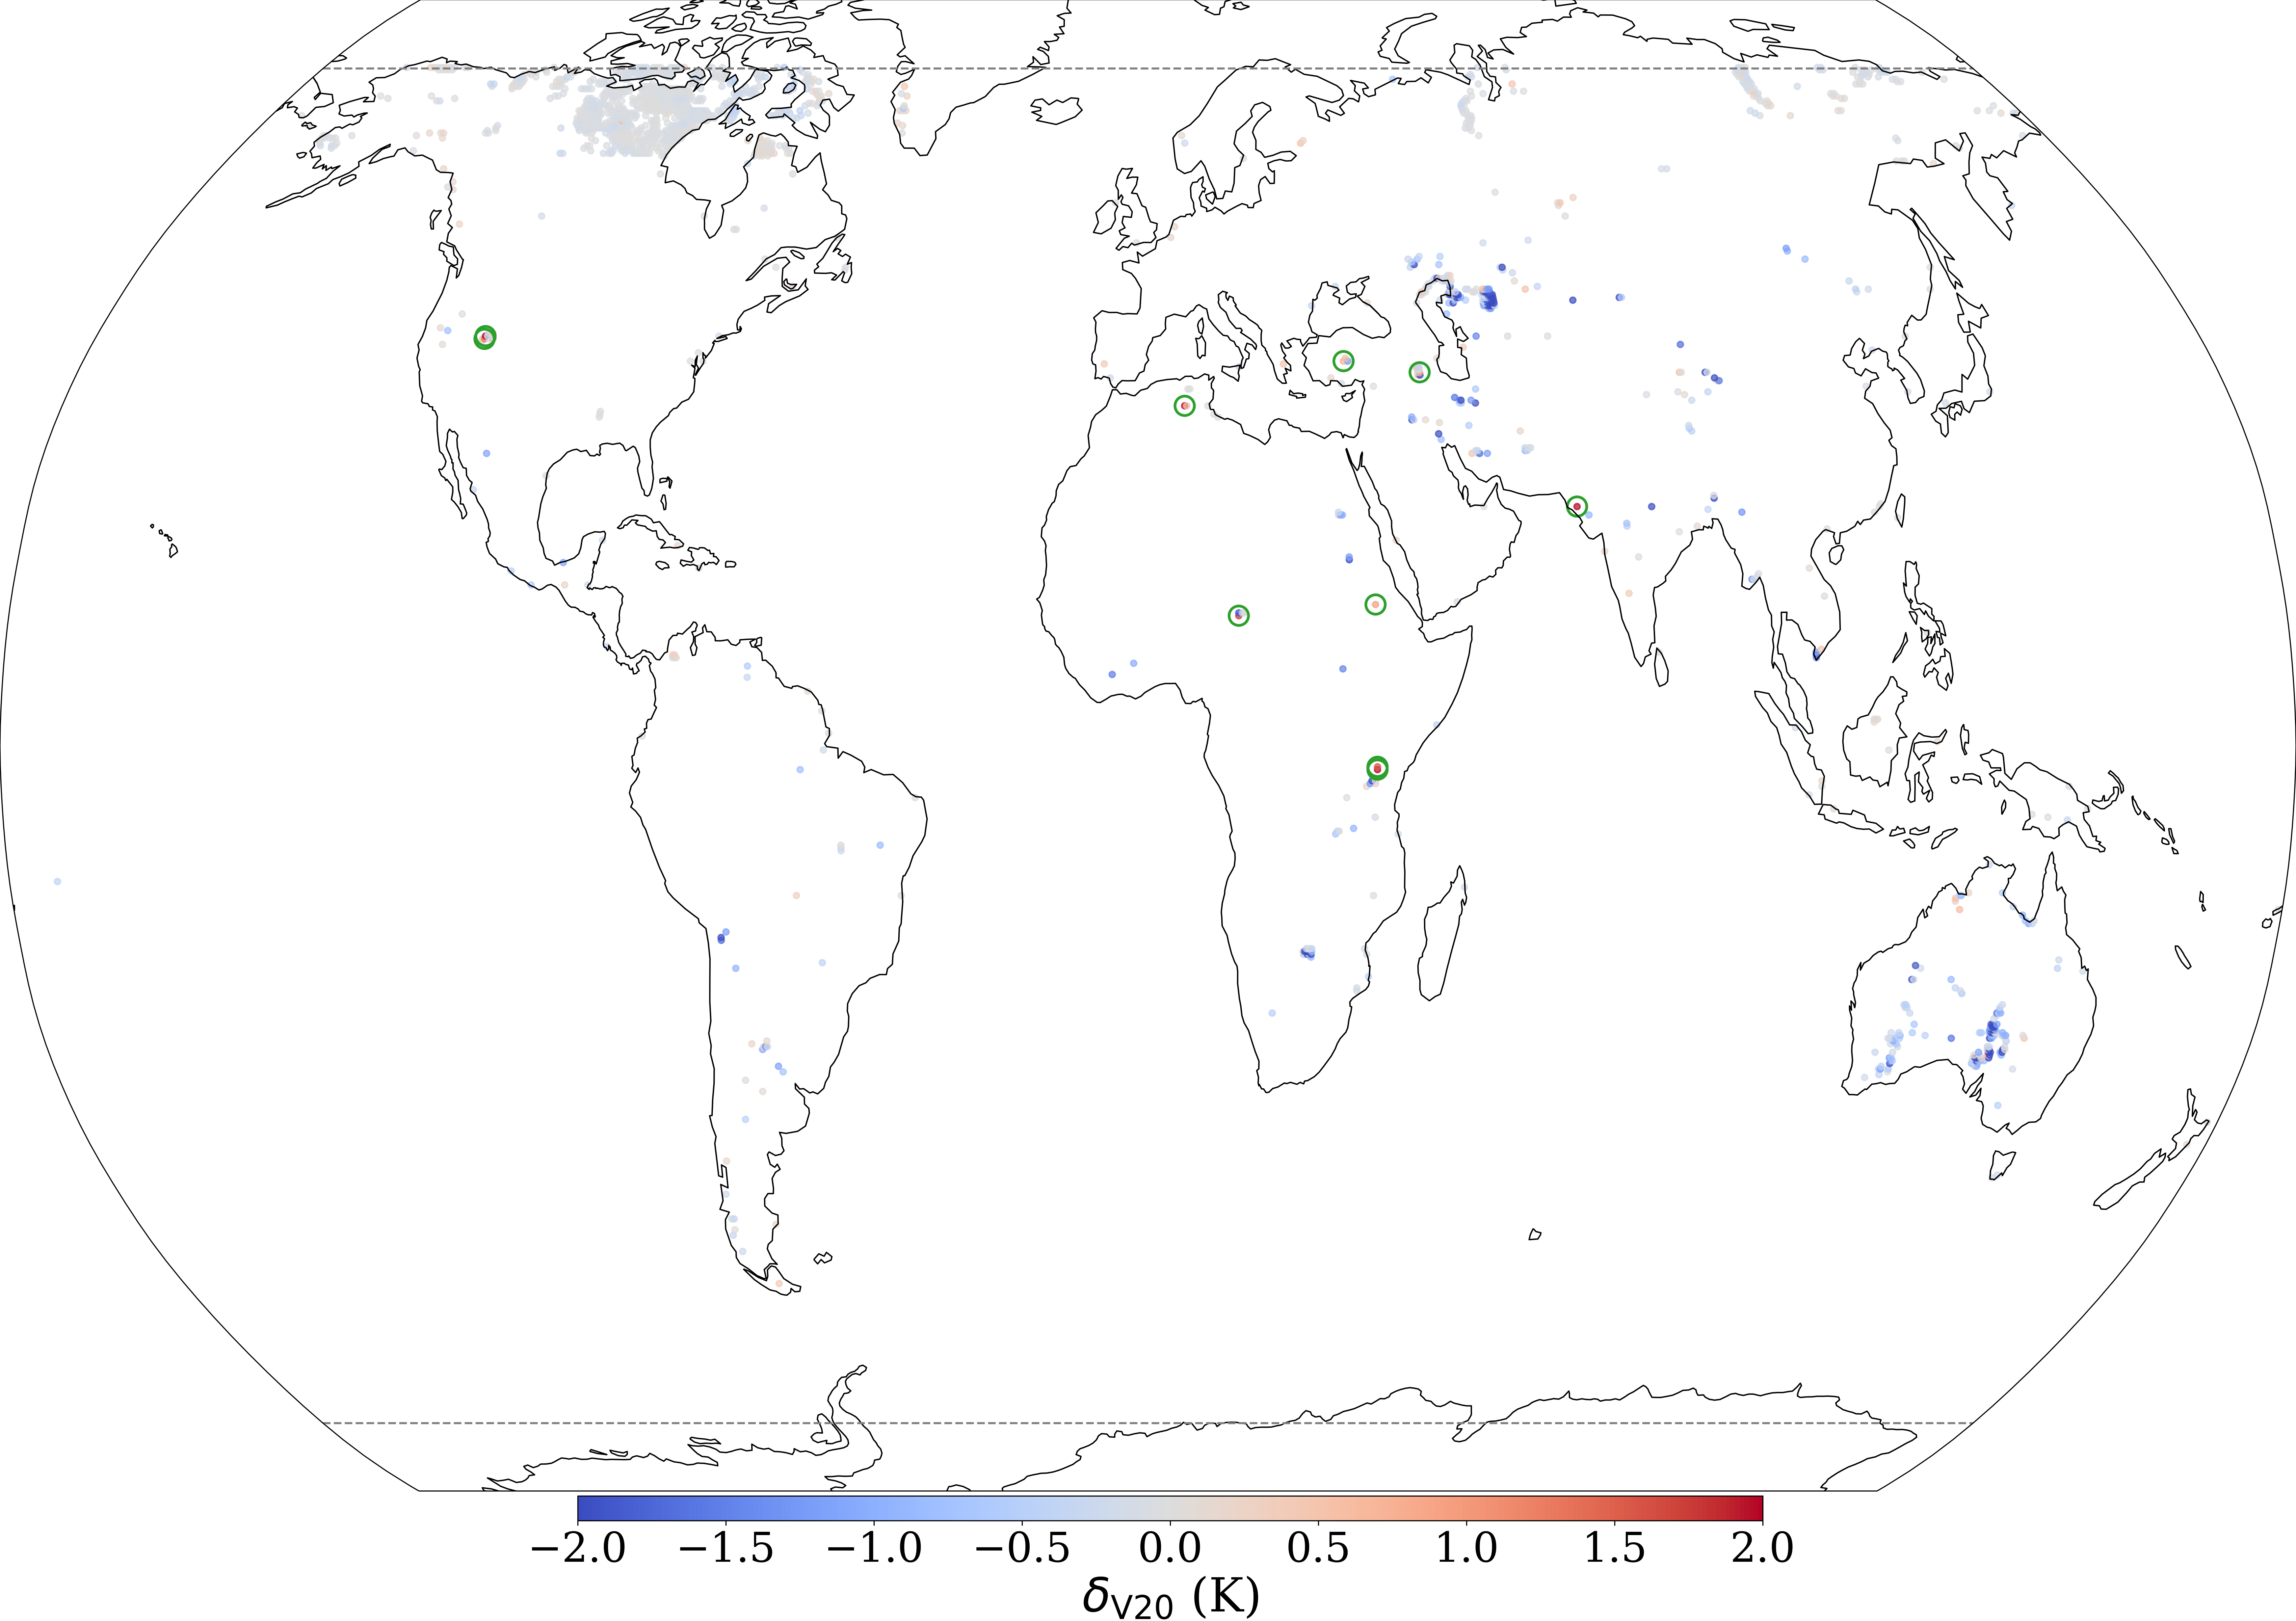
\includegraphics[width=0.98\textwidth]{updated_lakes_plot}
	\caption{\DIFaddFL{Differences in the prediction error MAE, between VESPER\_V20 and VESPER\_V15, (i.e. $\delta_{\rm V20}$),for 2019 at ~31km resolution for ‘Lake Updates’ category (i.e. where lake cover changed significantly). Generally, VESPER\_V20 LST predictions are more accurate, for example in the Aral sea and Australia, indicating that V20 field set is informative and accurate. Particular points where VESPER\_V20 LST prediction gets notably worse compared to VESPER\_V15 are highlighted with green circles and discussed in the text.}}
	\label{fig:bitstring_100110}
\end{figure*}

\DIFaddend \begin{figure*}
	\centering
	\DIFdelbeginFL %DIFDELCMD < \subfloat[Lake Natron, Tanzania \label{fig:lakes1}]{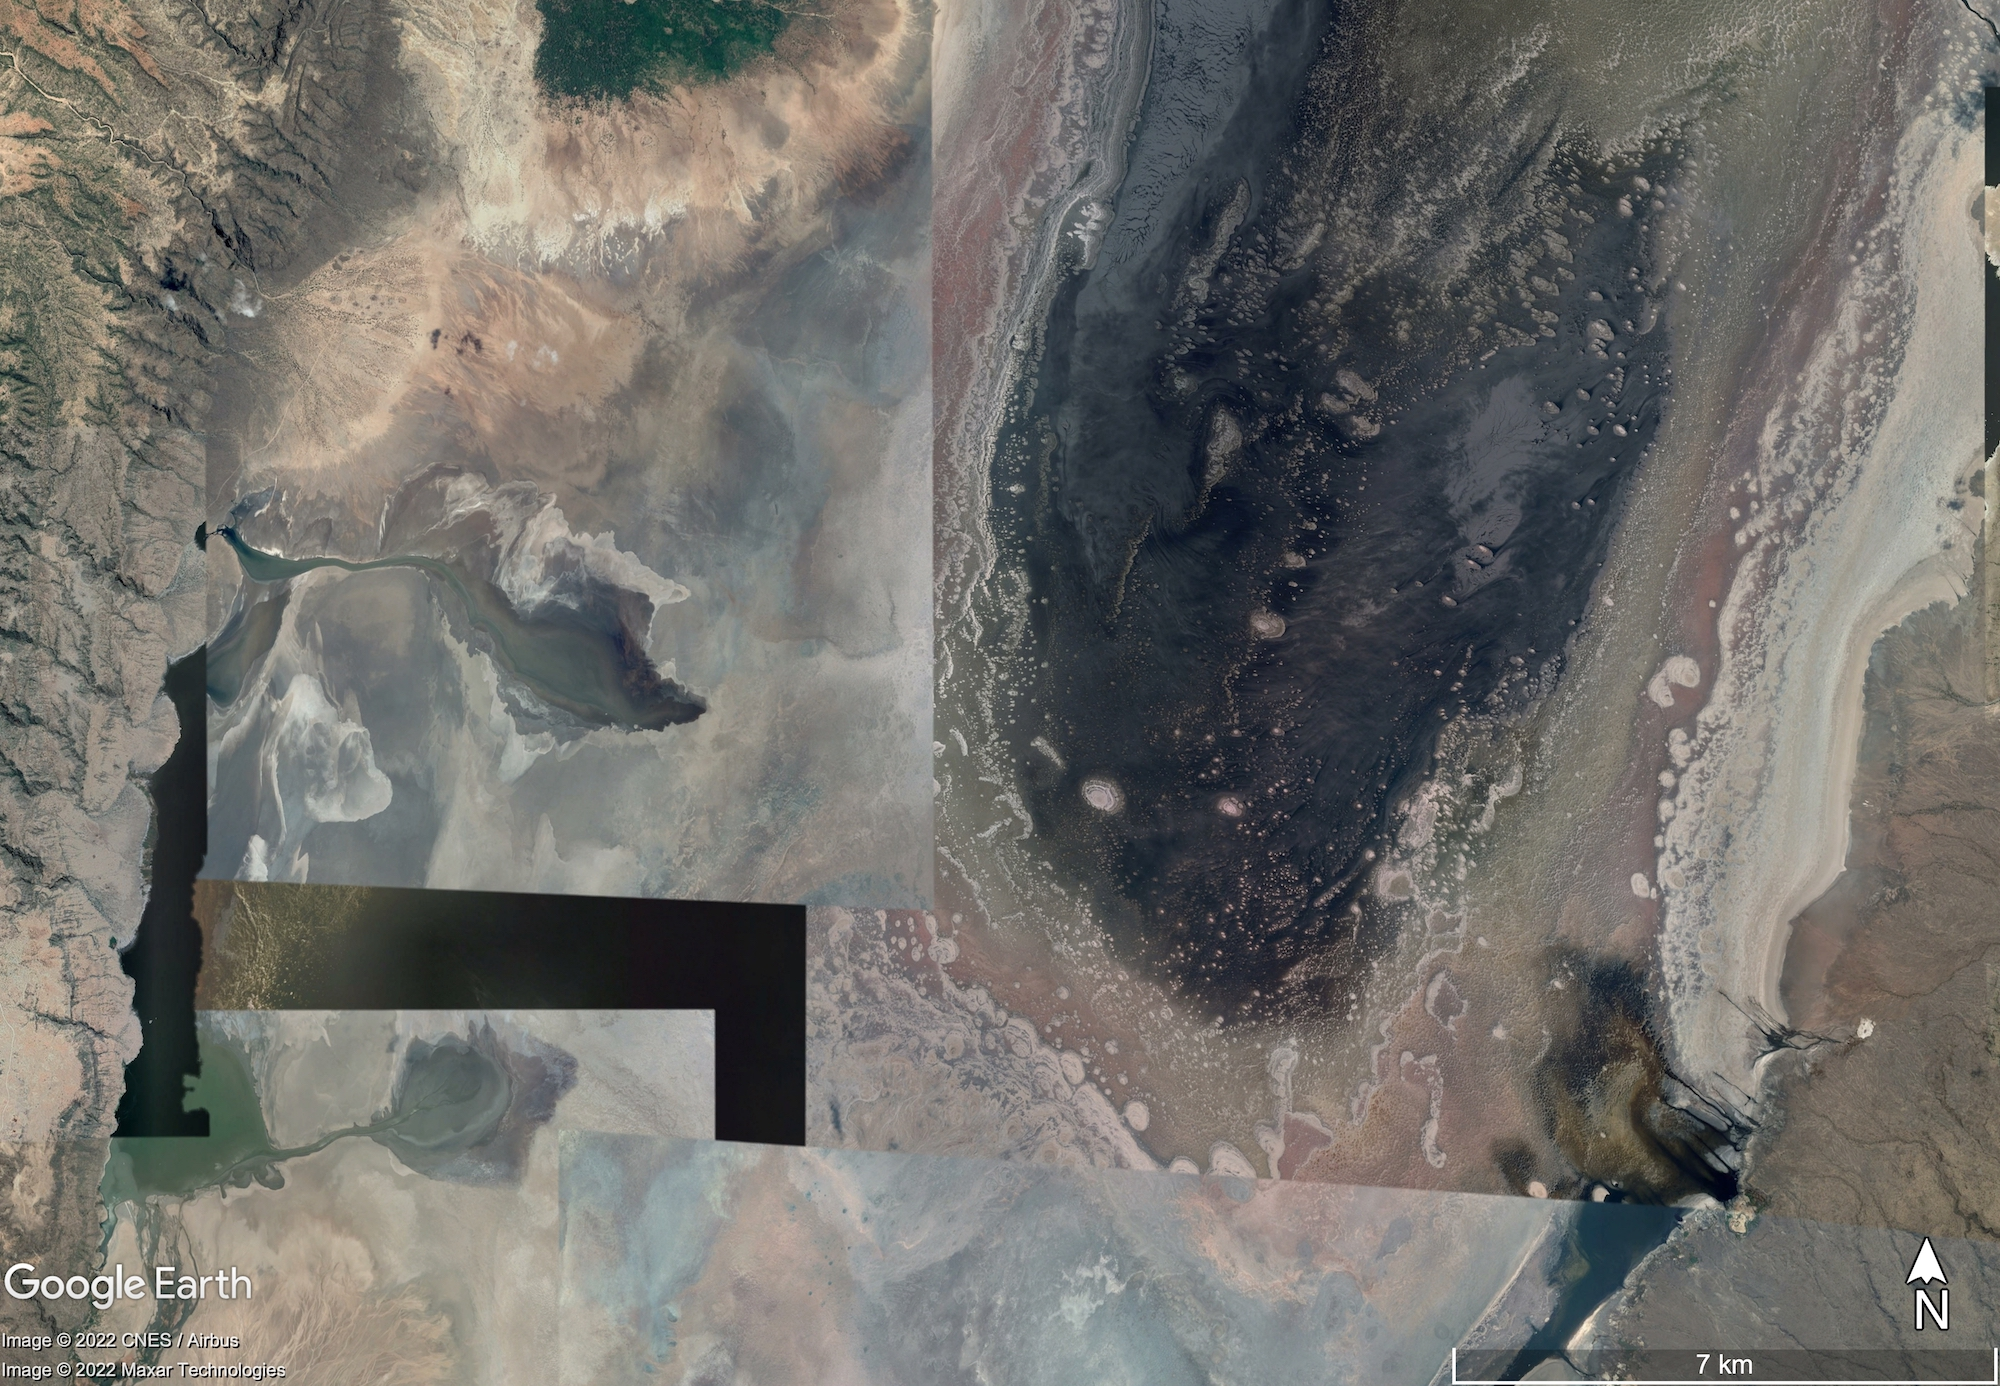
\includegraphics[width=0.45\textwidth]{LakeNatronCentre4.jpg}} %%%
\DIFdelFL{\hspace{1mm}
	}%DIFDELCMD < \subfloat[Lake Blanche, Australia \label{fig:lakes2}]{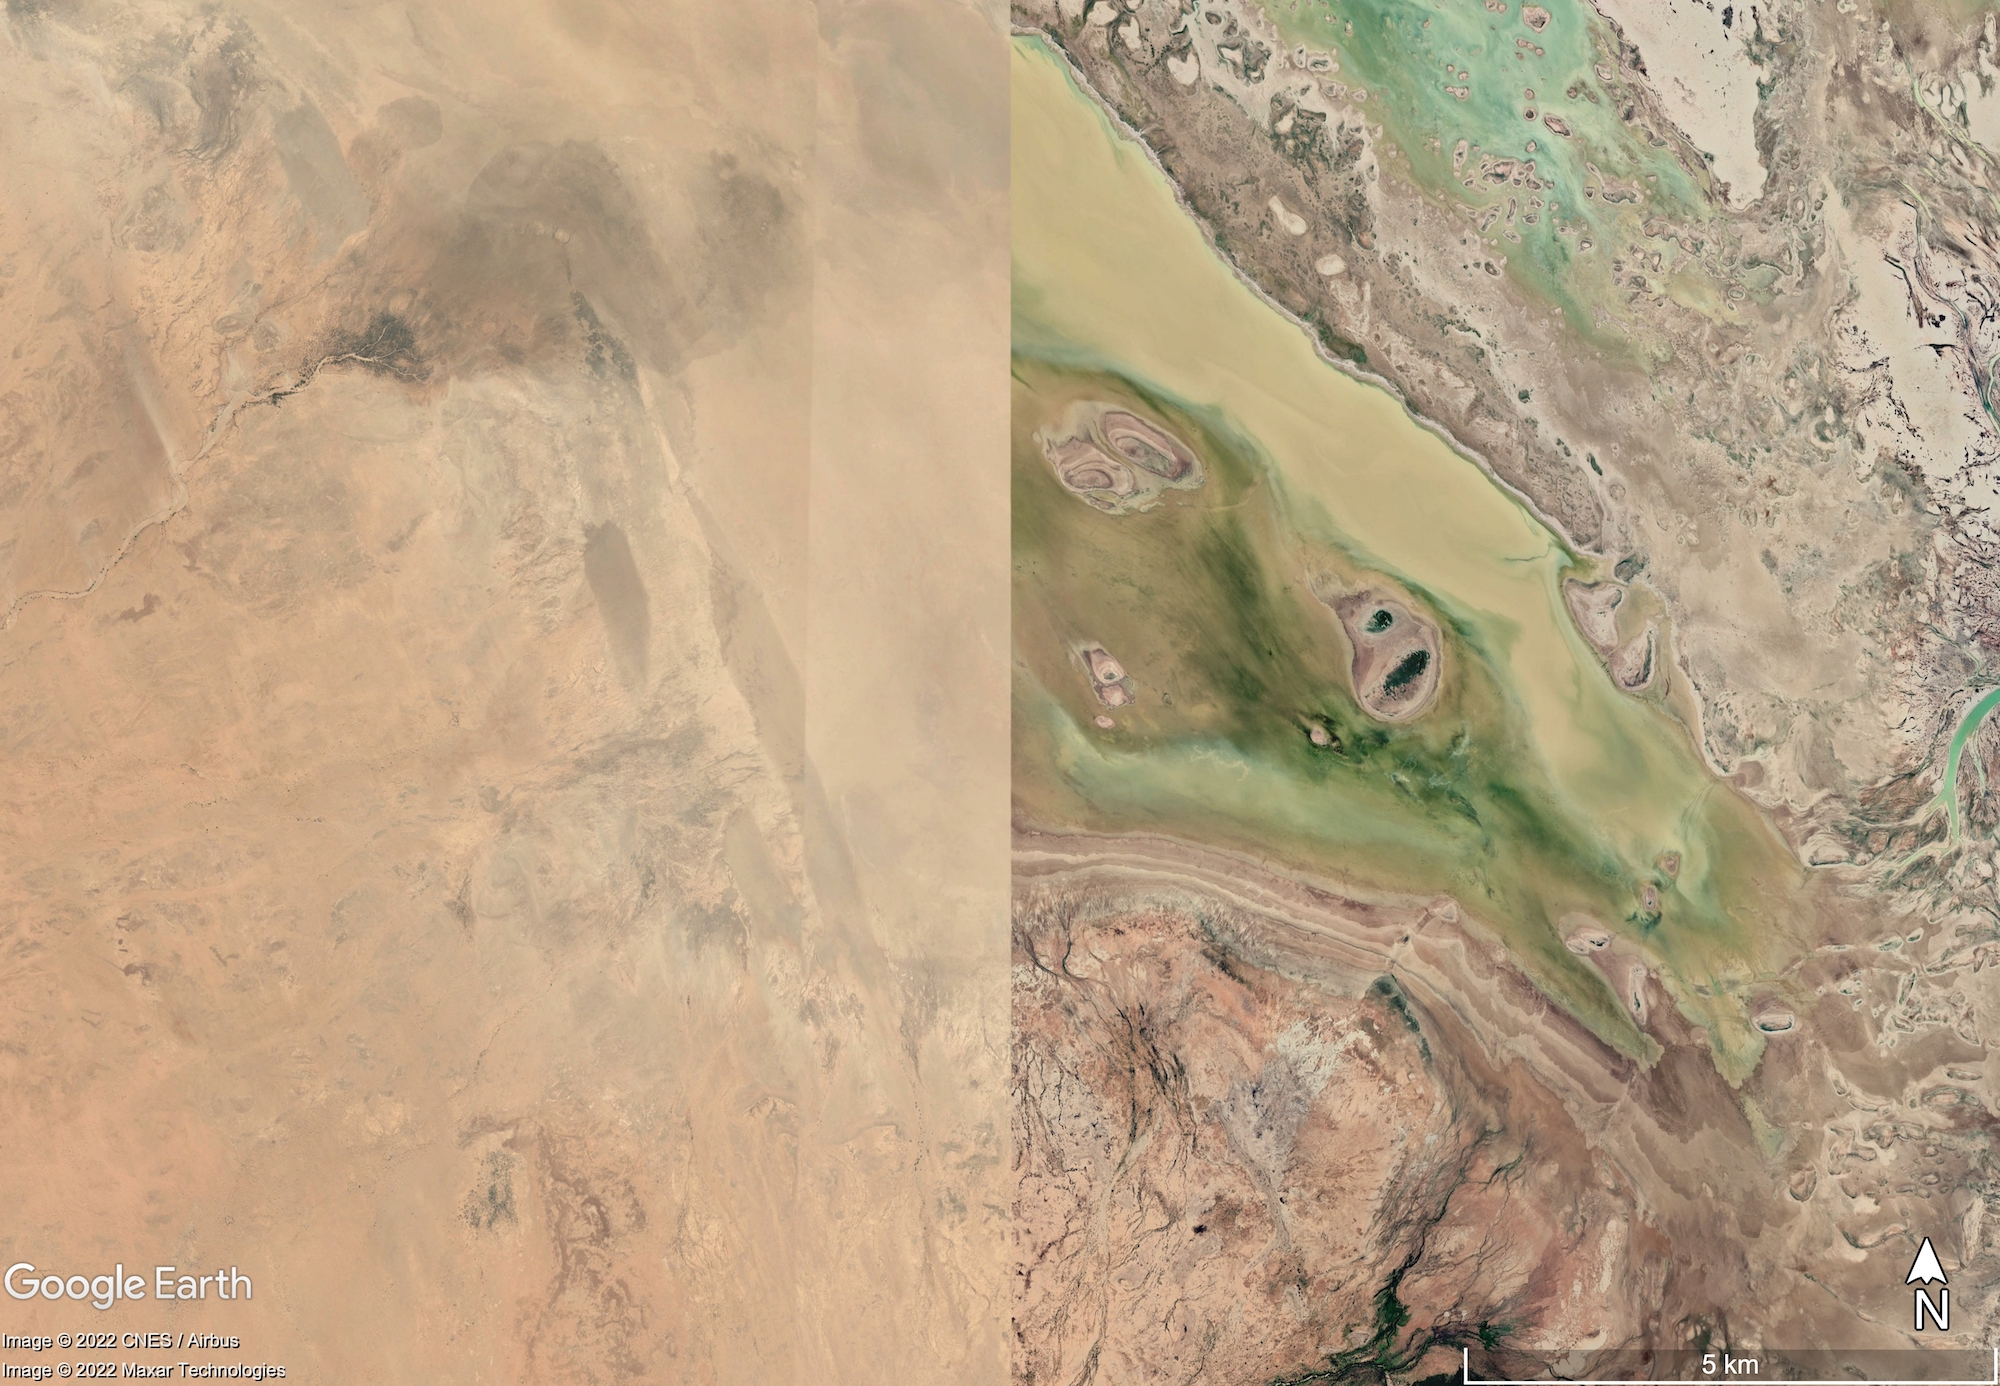
\includegraphics[width=0.45\textwidth]{Australia1}} %%%
\DIFdelendFL \DIFaddbeginFL \subfloat[Gujarat Province, India\label{fig:lakes5}]{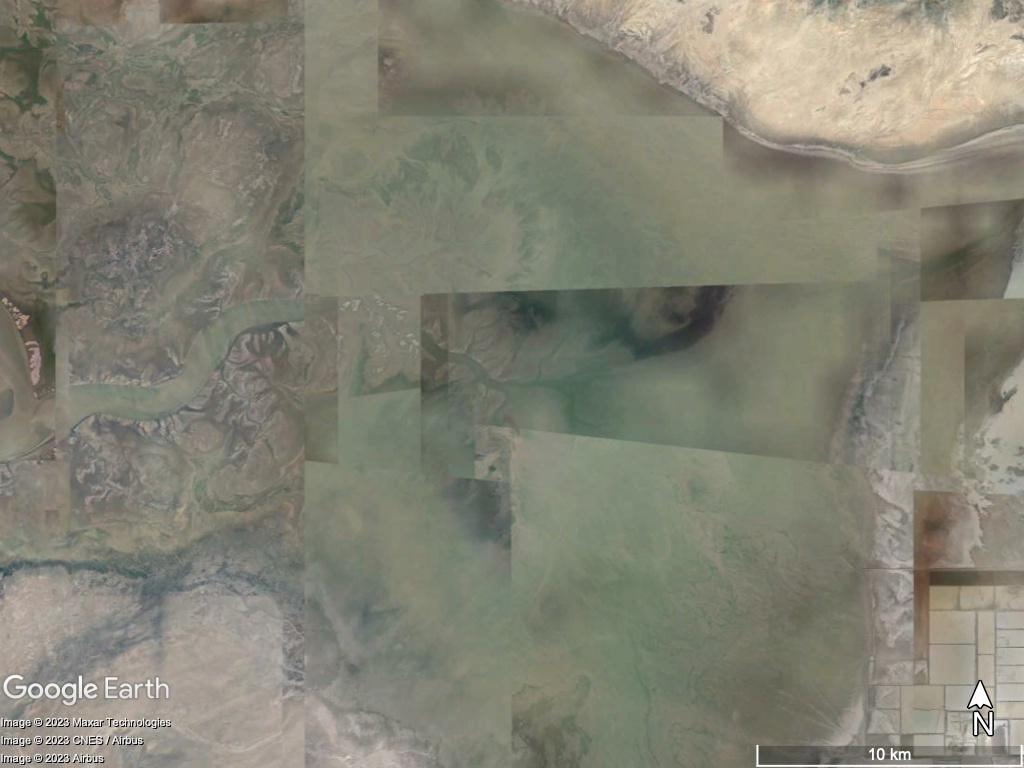
\includegraphics[width=0.45\textwidth]{gujarat_bonus}} \DIFaddFL{\hspace{1mm}
	}\subfloat[Great Salt Lake Desert, Utah\label{fig:lakes3}]{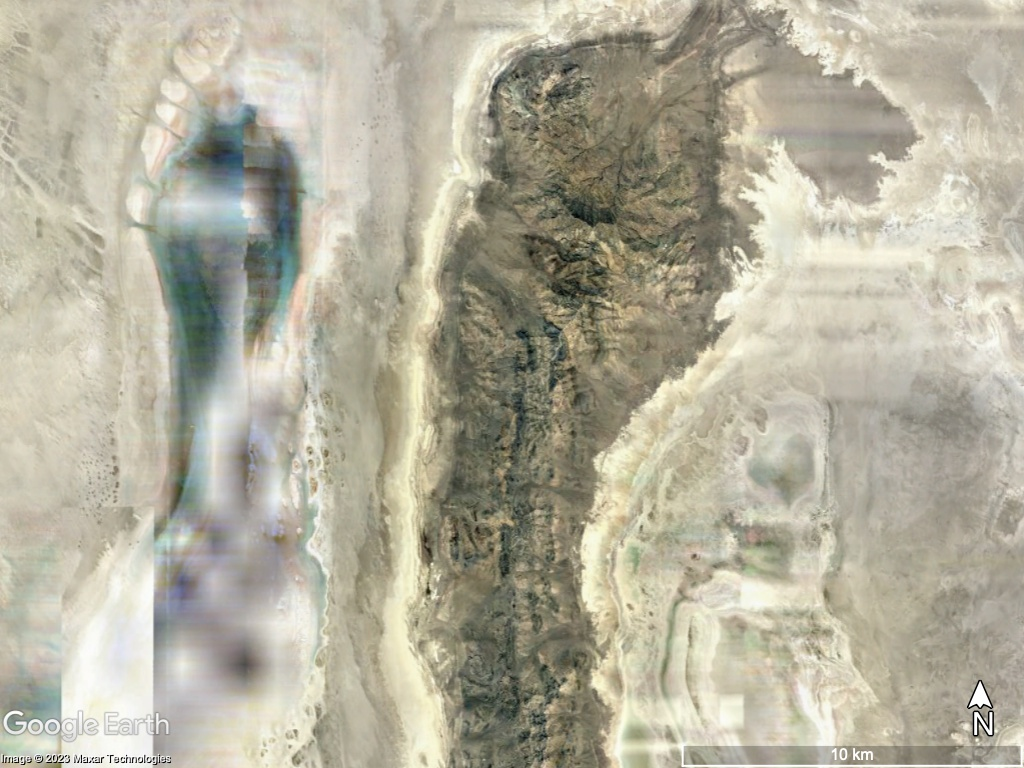
\includegraphics[width=0.45\textwidth]{SLC_bonus}} \DIFaddFL{\hspace{1mm} }\DIFaddendFL \\
	\DIFdelbeginFL %DIFDELCMD < \subfloat[Great Salt Lake Desert, Utah\label{fig:lakes3}]{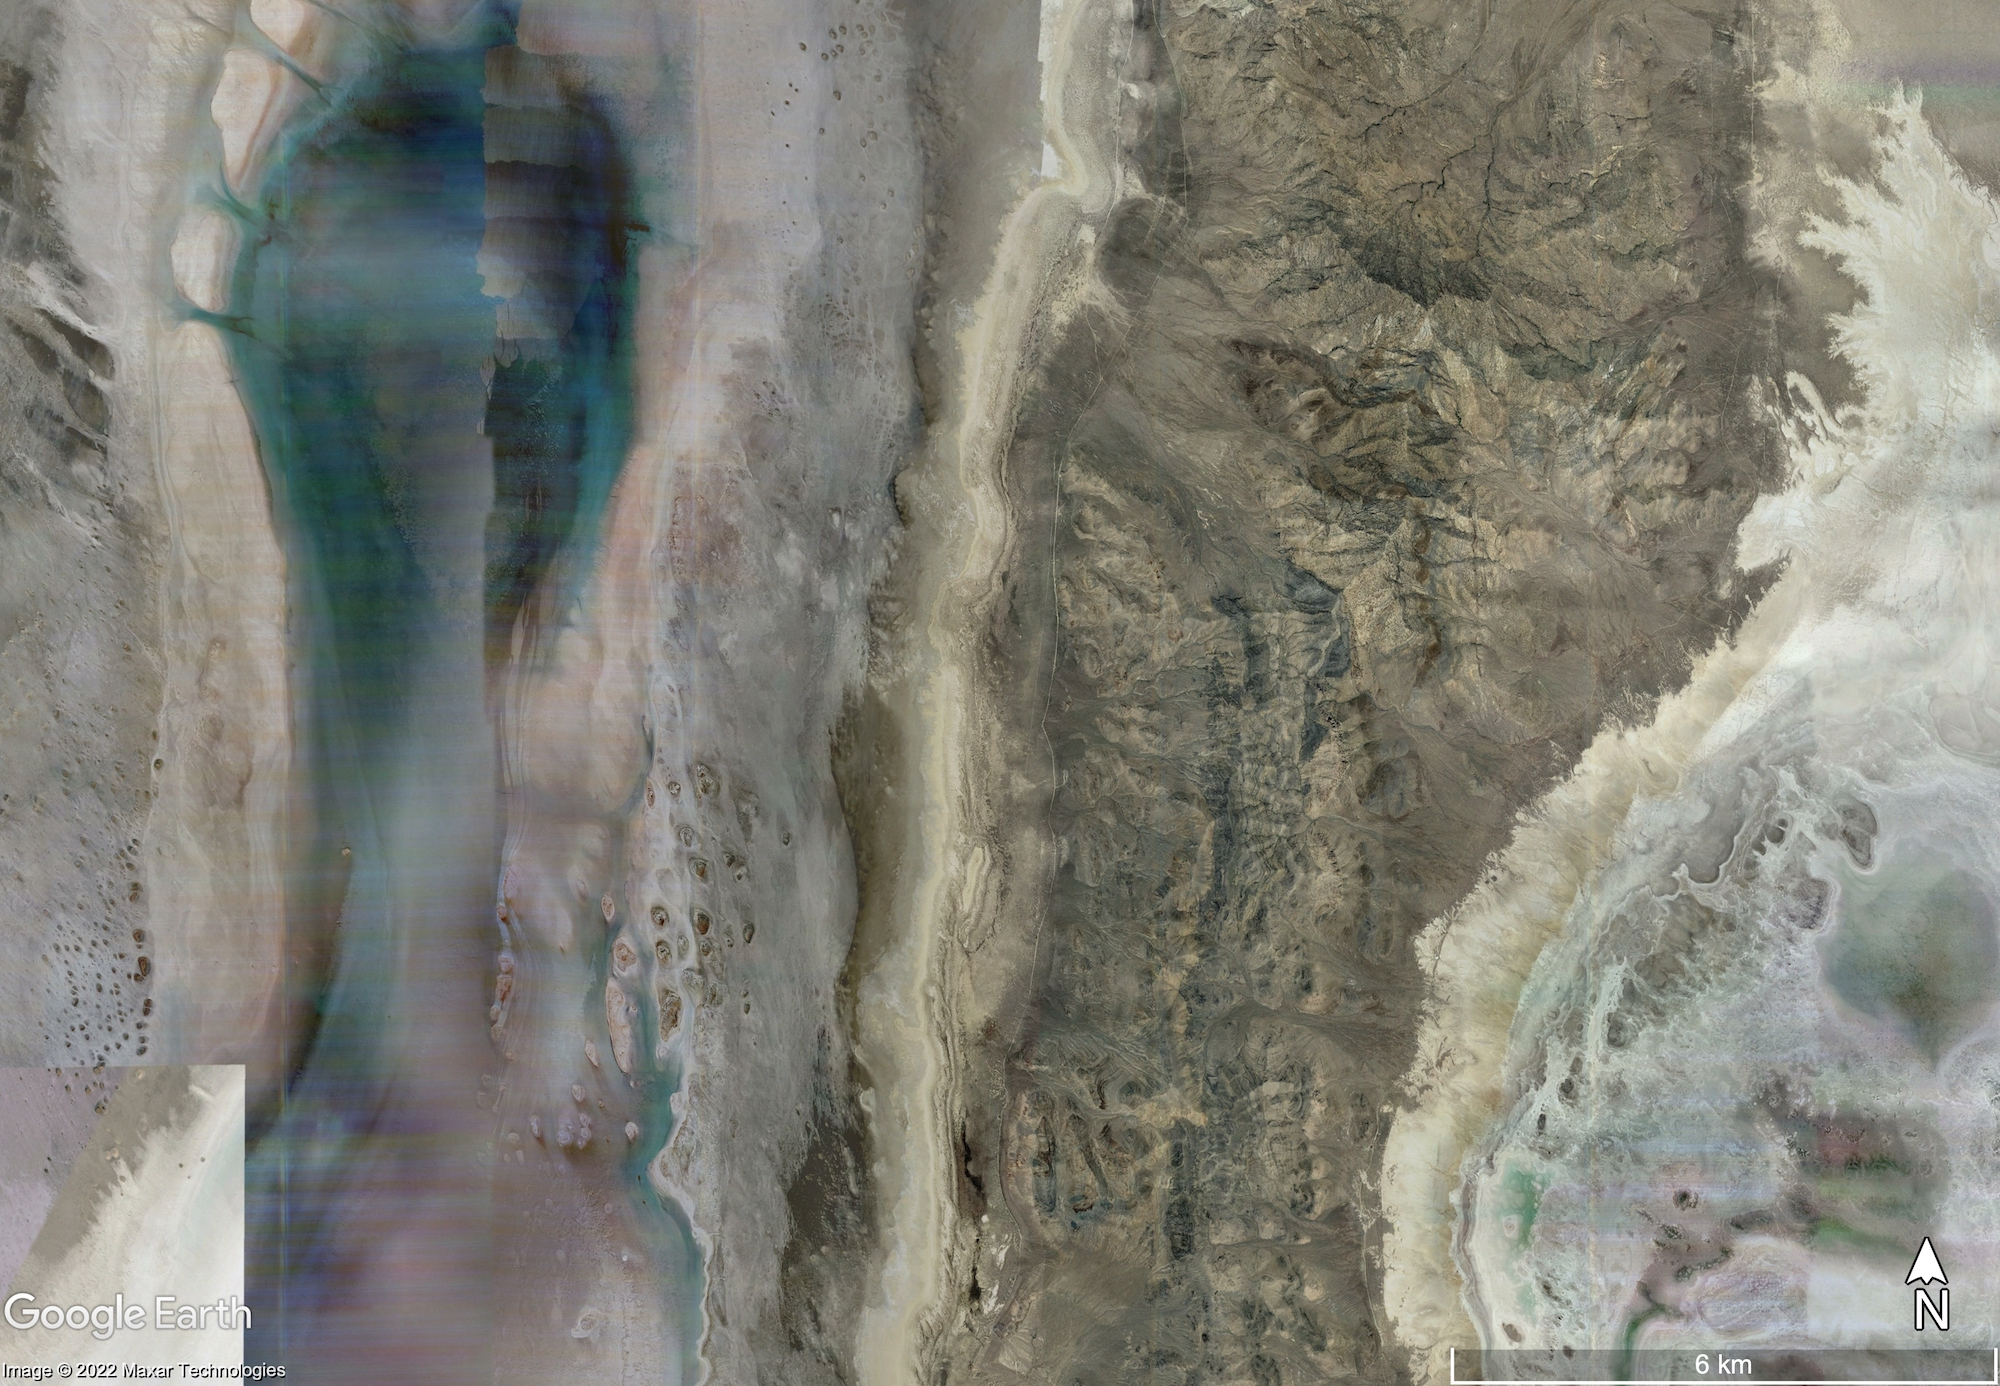
\includegraphics[width=0.45\textwidth]{SLC1.jpg}} %%%
\DIFdelFL{\hspace{1mm}
	}%DIFDELCMD < \subfloat[Farah Province, Afghanistan\label{fig:lakes4}]{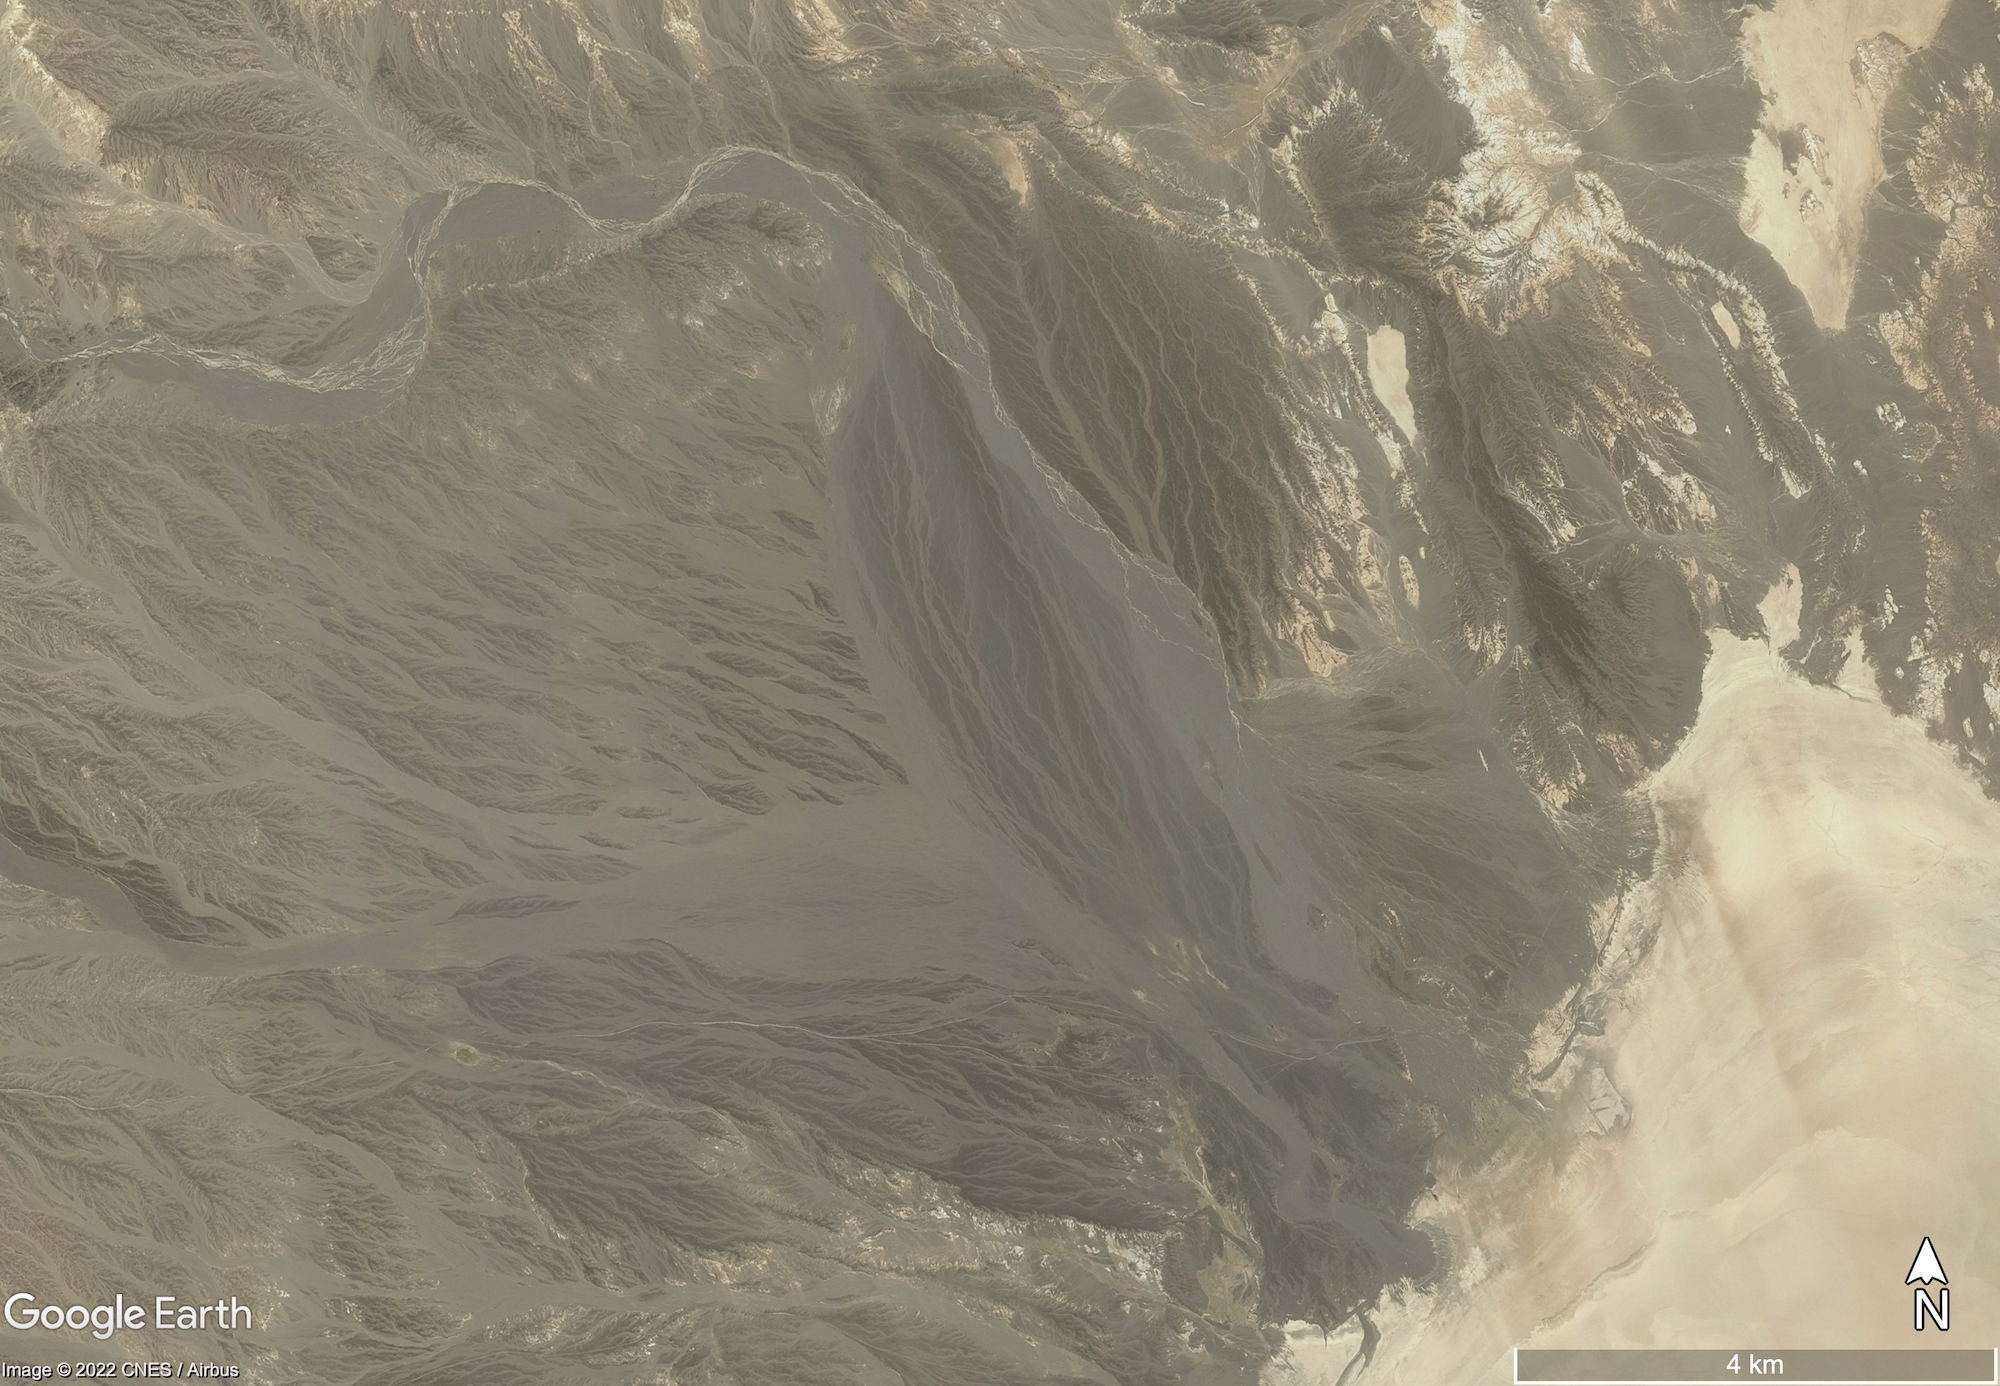
\includegraphics[width=0.45\textwidth]{Afghan1}} %%%
\DIFdelendFL \DIFaddbeginFL \subfloat[Lake Natron, Tanzania \label{fig:lakes1}]{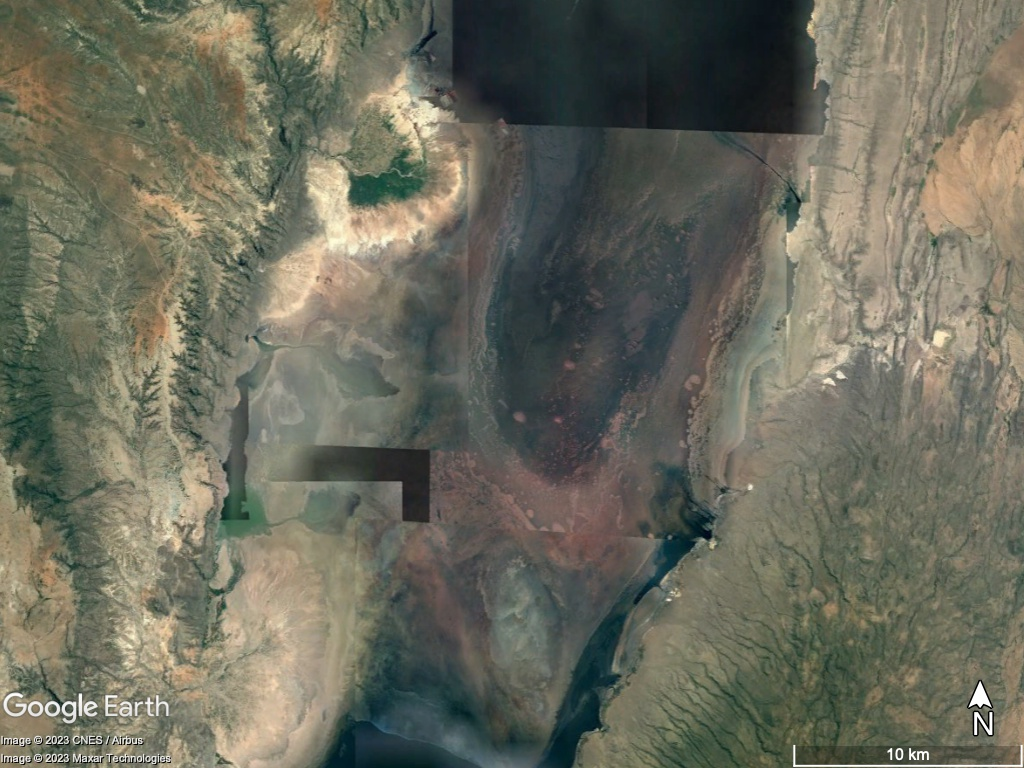
\includegraphics[width=0.45\textwidth]{lake_natron_bonus}} \DIFaddFL{\hspace{1mm}
	}\subfloat[Lake Tersakan/Lake Tuz \label{fig:lakes44s}]{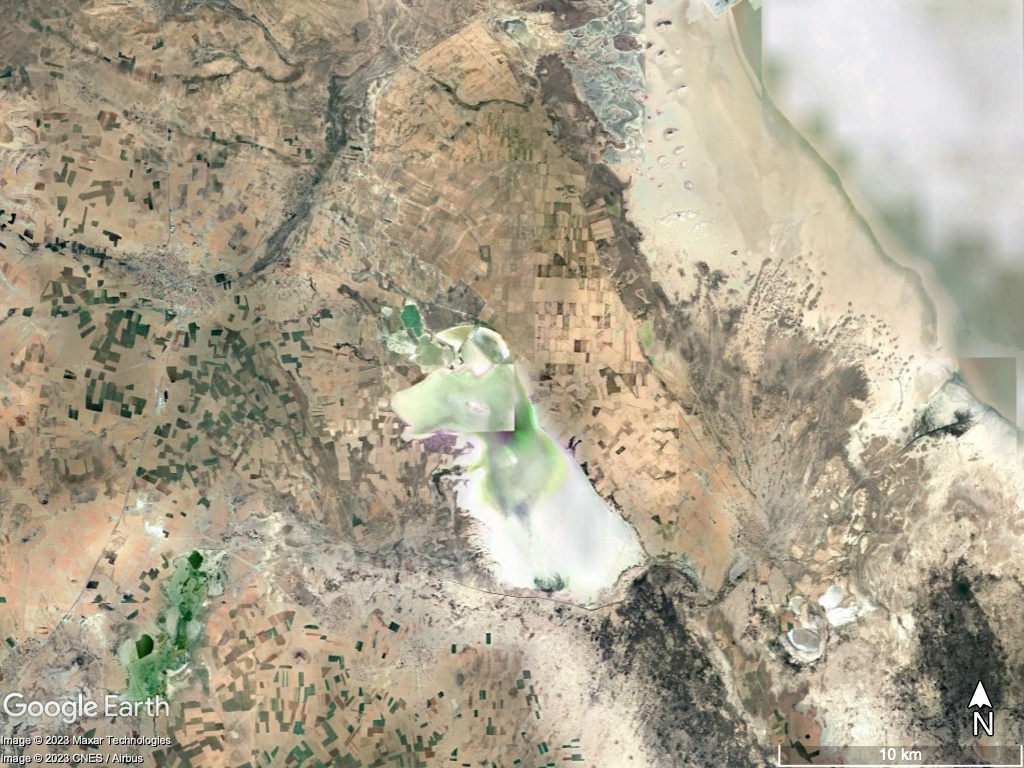
\includegraphics[width=0.45\textwidth]{lake_tuz}} \DIFaddFL{\hspace{1mm} }\DIFaddendFL \\
	\DIFdelbeginFL %DIFDELCMD < \subfloat[Gujarat Province, India\label{fig:lakes5}]{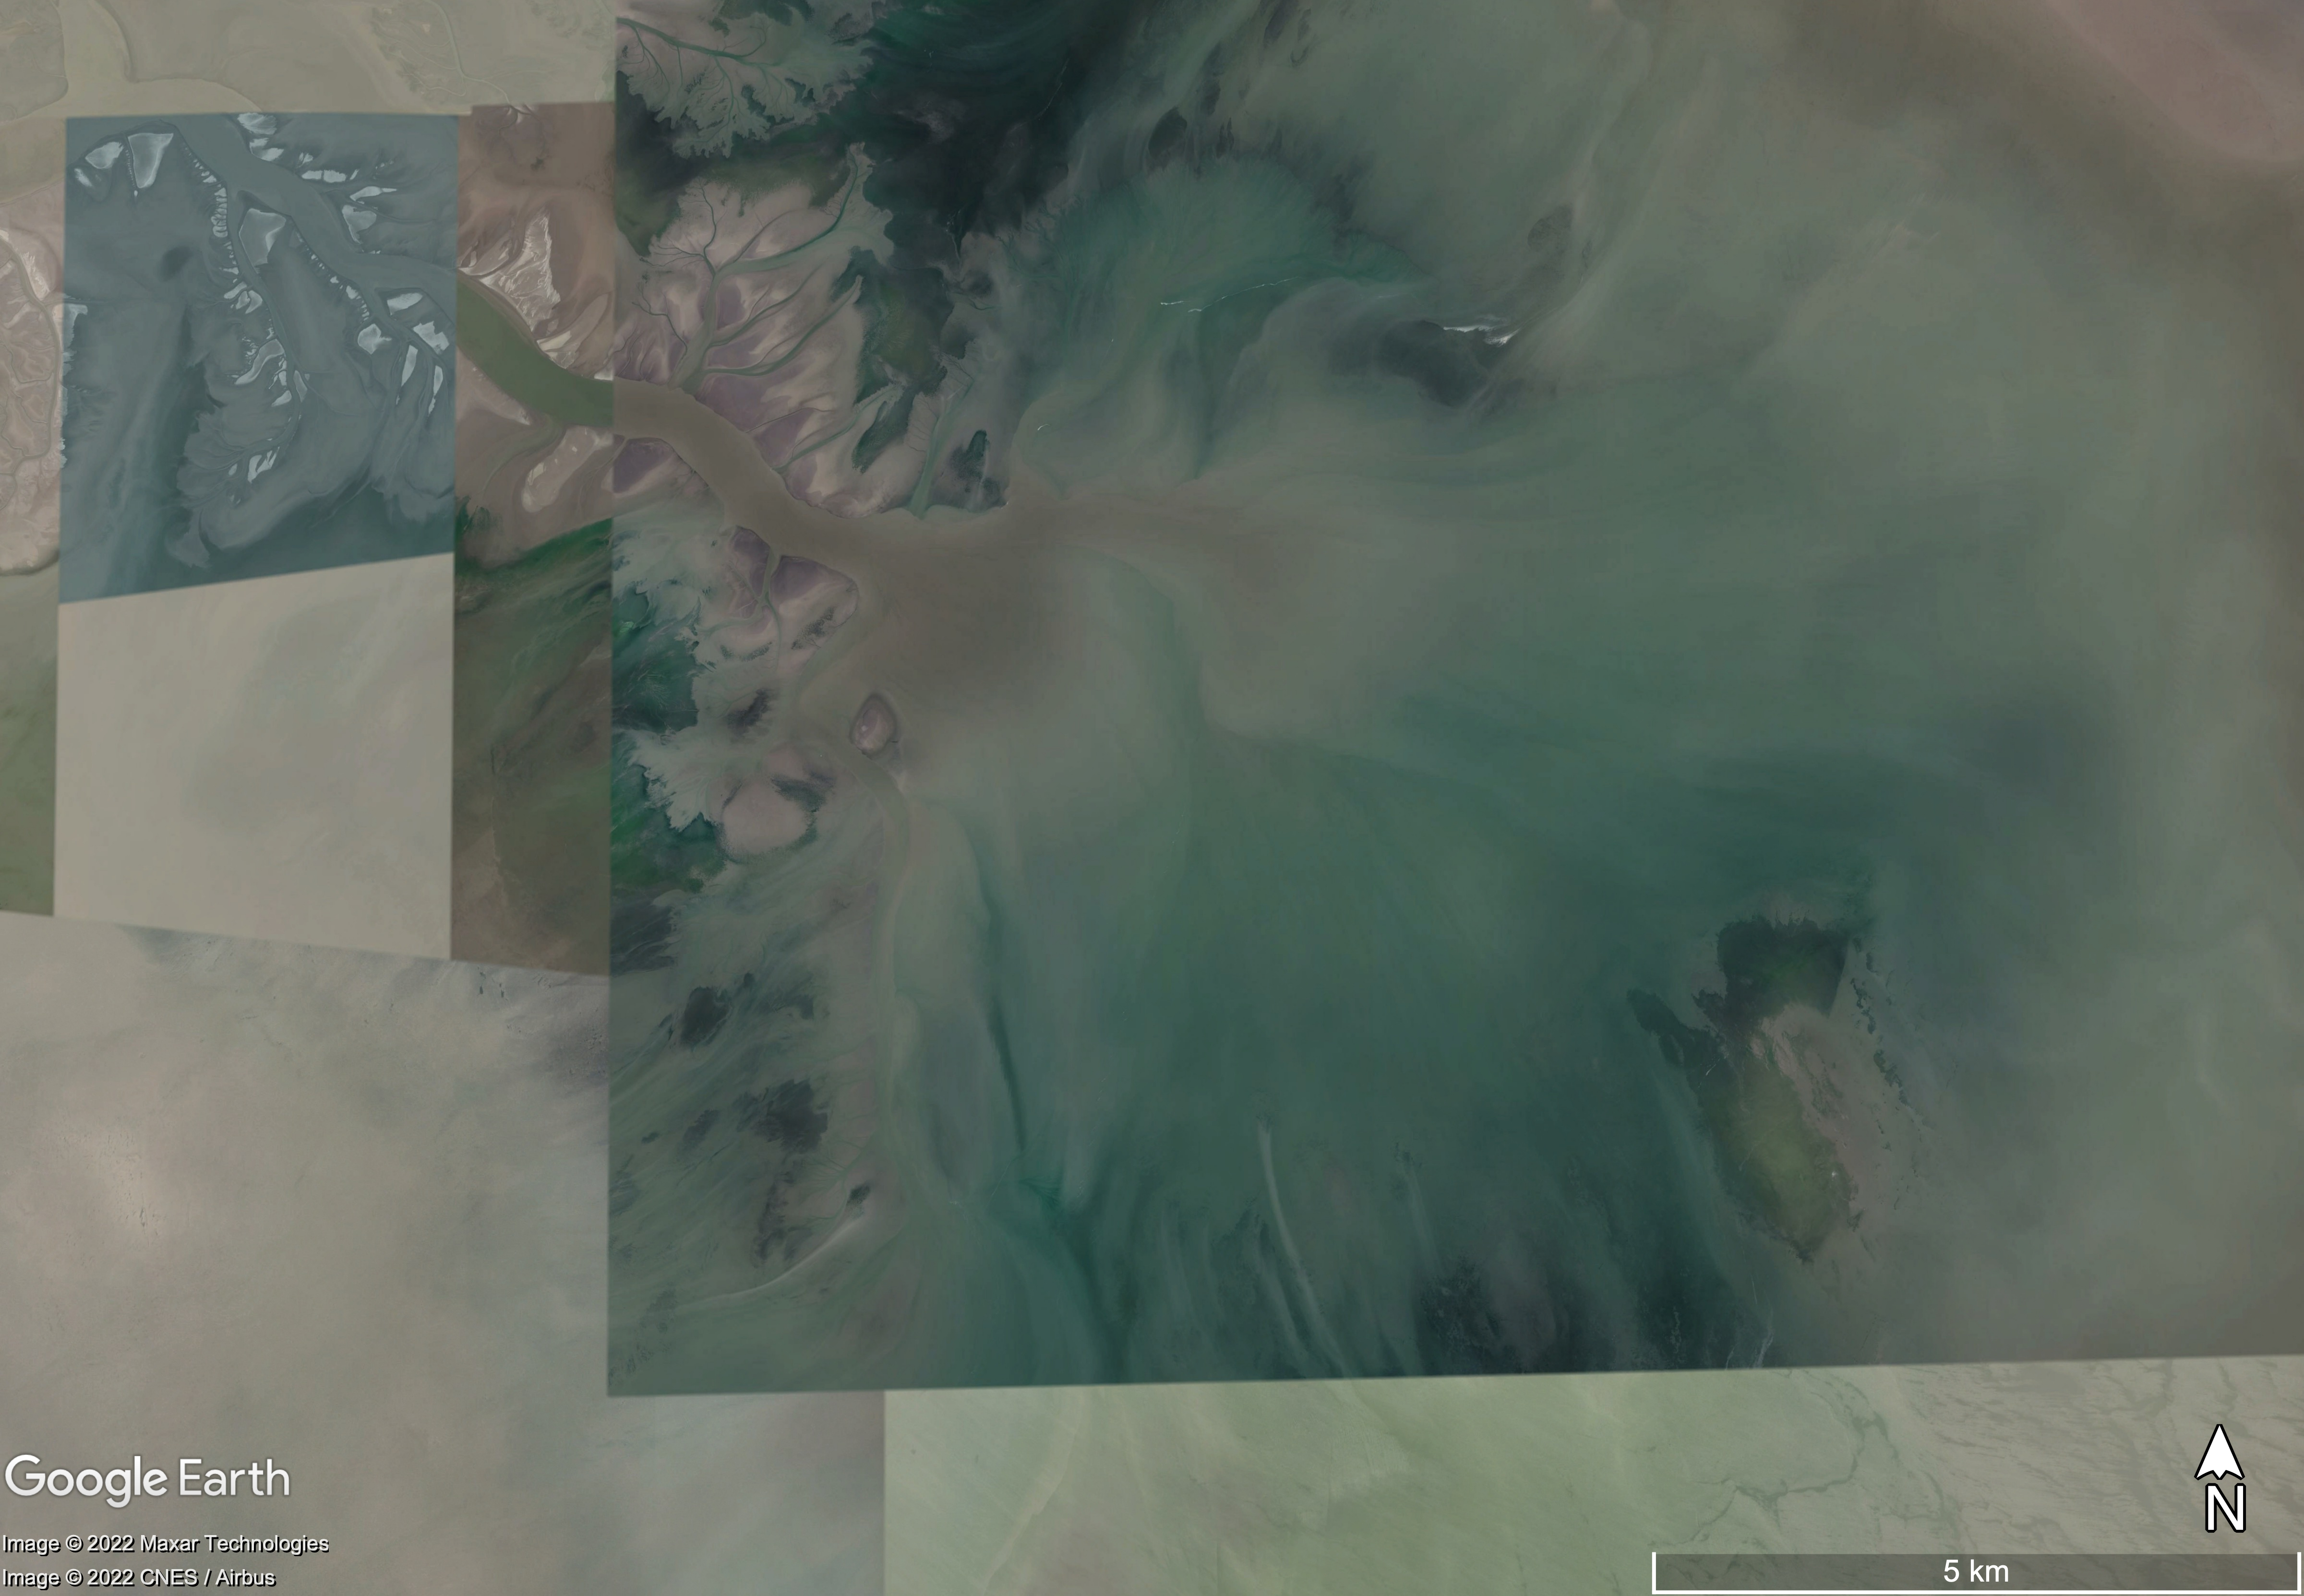
\includegraphics[width=0.45\textwidth]{India1.jpg}} %%%
\DIFdelFL{\hspace{1mm}
	}%DIFDELCMD < \subfloat[Toshka Lakes, Egypt\label{fig:lakes6}]{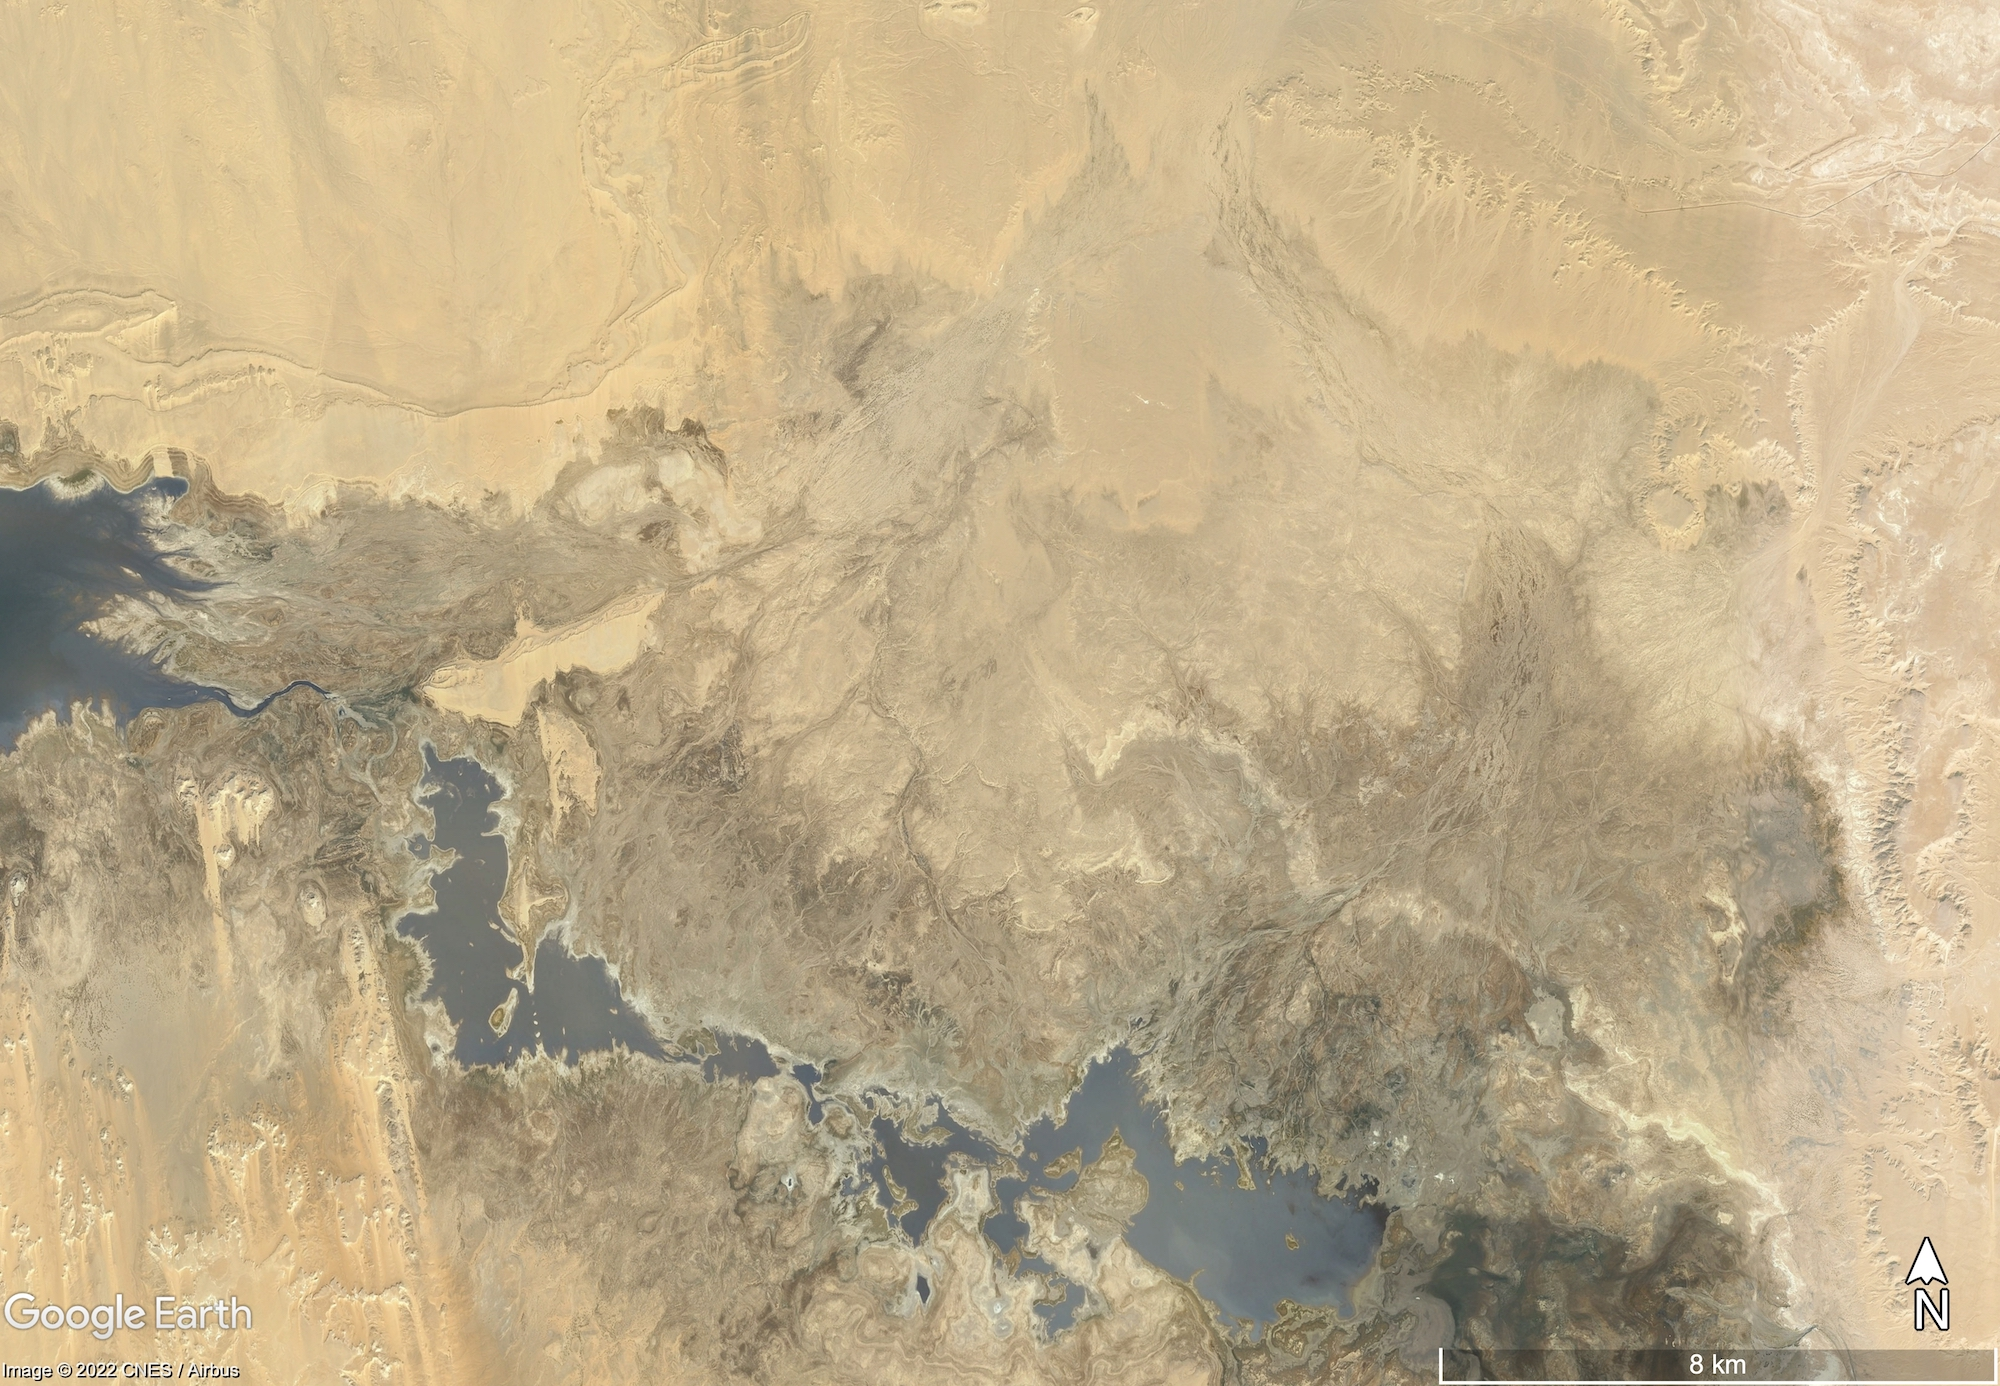
\includegraphics[width=0.45\textwidth]{Egypt1}}
%DIFDELCMD < 	%%%
\DIFdelendFL \DIFaddbeginFL \subfloat[Lake Chad \label{fig:lakes11}]{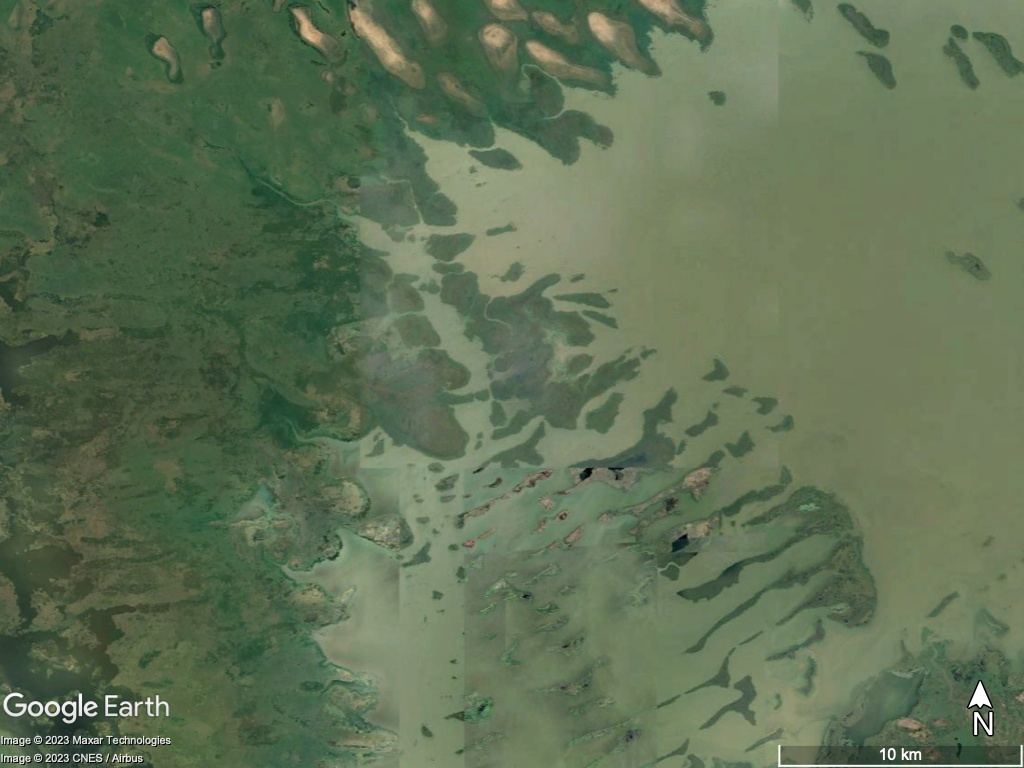
\includegraphics[width=0.45\textwidth]{lake_chad}} \DIFaddFL{\hspace{1mm}
	}\subfloat[Lake Urmia \label{fig:lakes444s}]{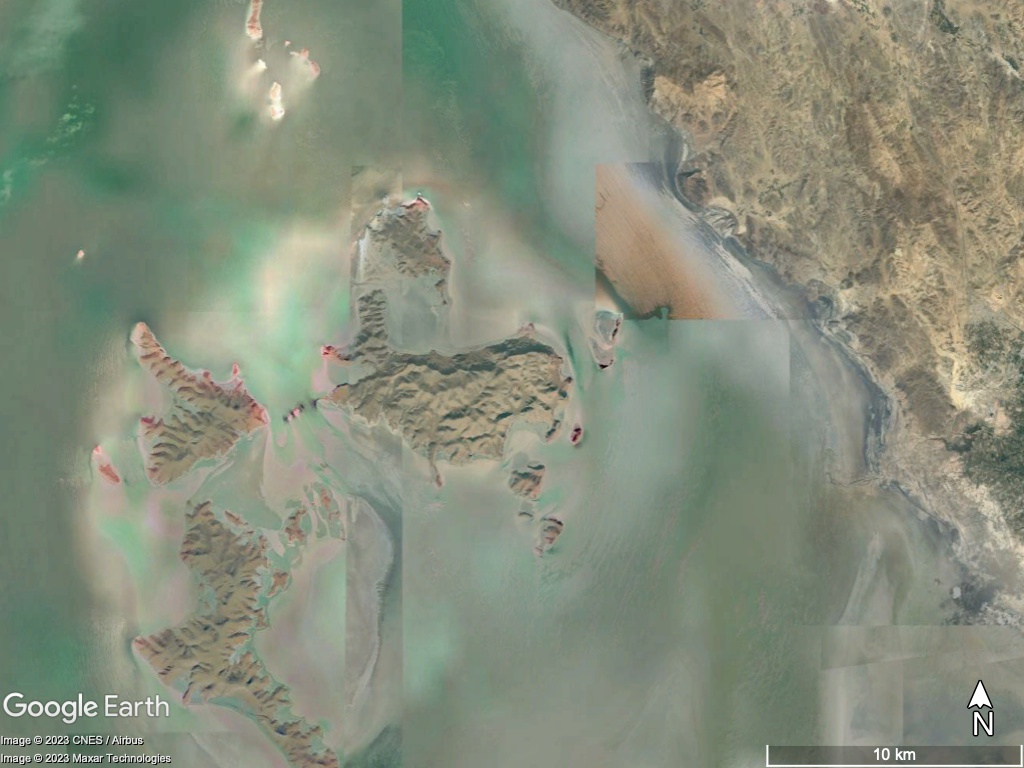
\includegraphics[width=0.45\textwidth]{lake_urmia}} \DIFaddFL{\hspace{1mm} }\\
	\DIFaddendFL \caption{\DIFdelbeginFL \DIFdelFL{Satellite }\DIFdelendFL \DIFaddbeginFL \DIFaddFL{A selection of satellite }\DIFaddendFL imagery of \DIFaddbeginFL \DIFaddFL{some of }\DIFaddendFL the problematic Lake Updates points highlighted in Fig. \ref{fig:bitstring_100110} where the V20 predictions are worse than the V15 predictions. Generally the updated V20 fields remove water, only considering permanent water. However these regions have highly time variable waters, which are better captured on average by the V15 fields. The images are centred on the grid box coordinates.\DIFdelbeginFL \DIFdelFL{Note that the lengthscales are different for some images.}\DIFdelendFL } 
	\label{fig:example_test}
\end{figure*}


\DIFaddbegin \begin{figure}
	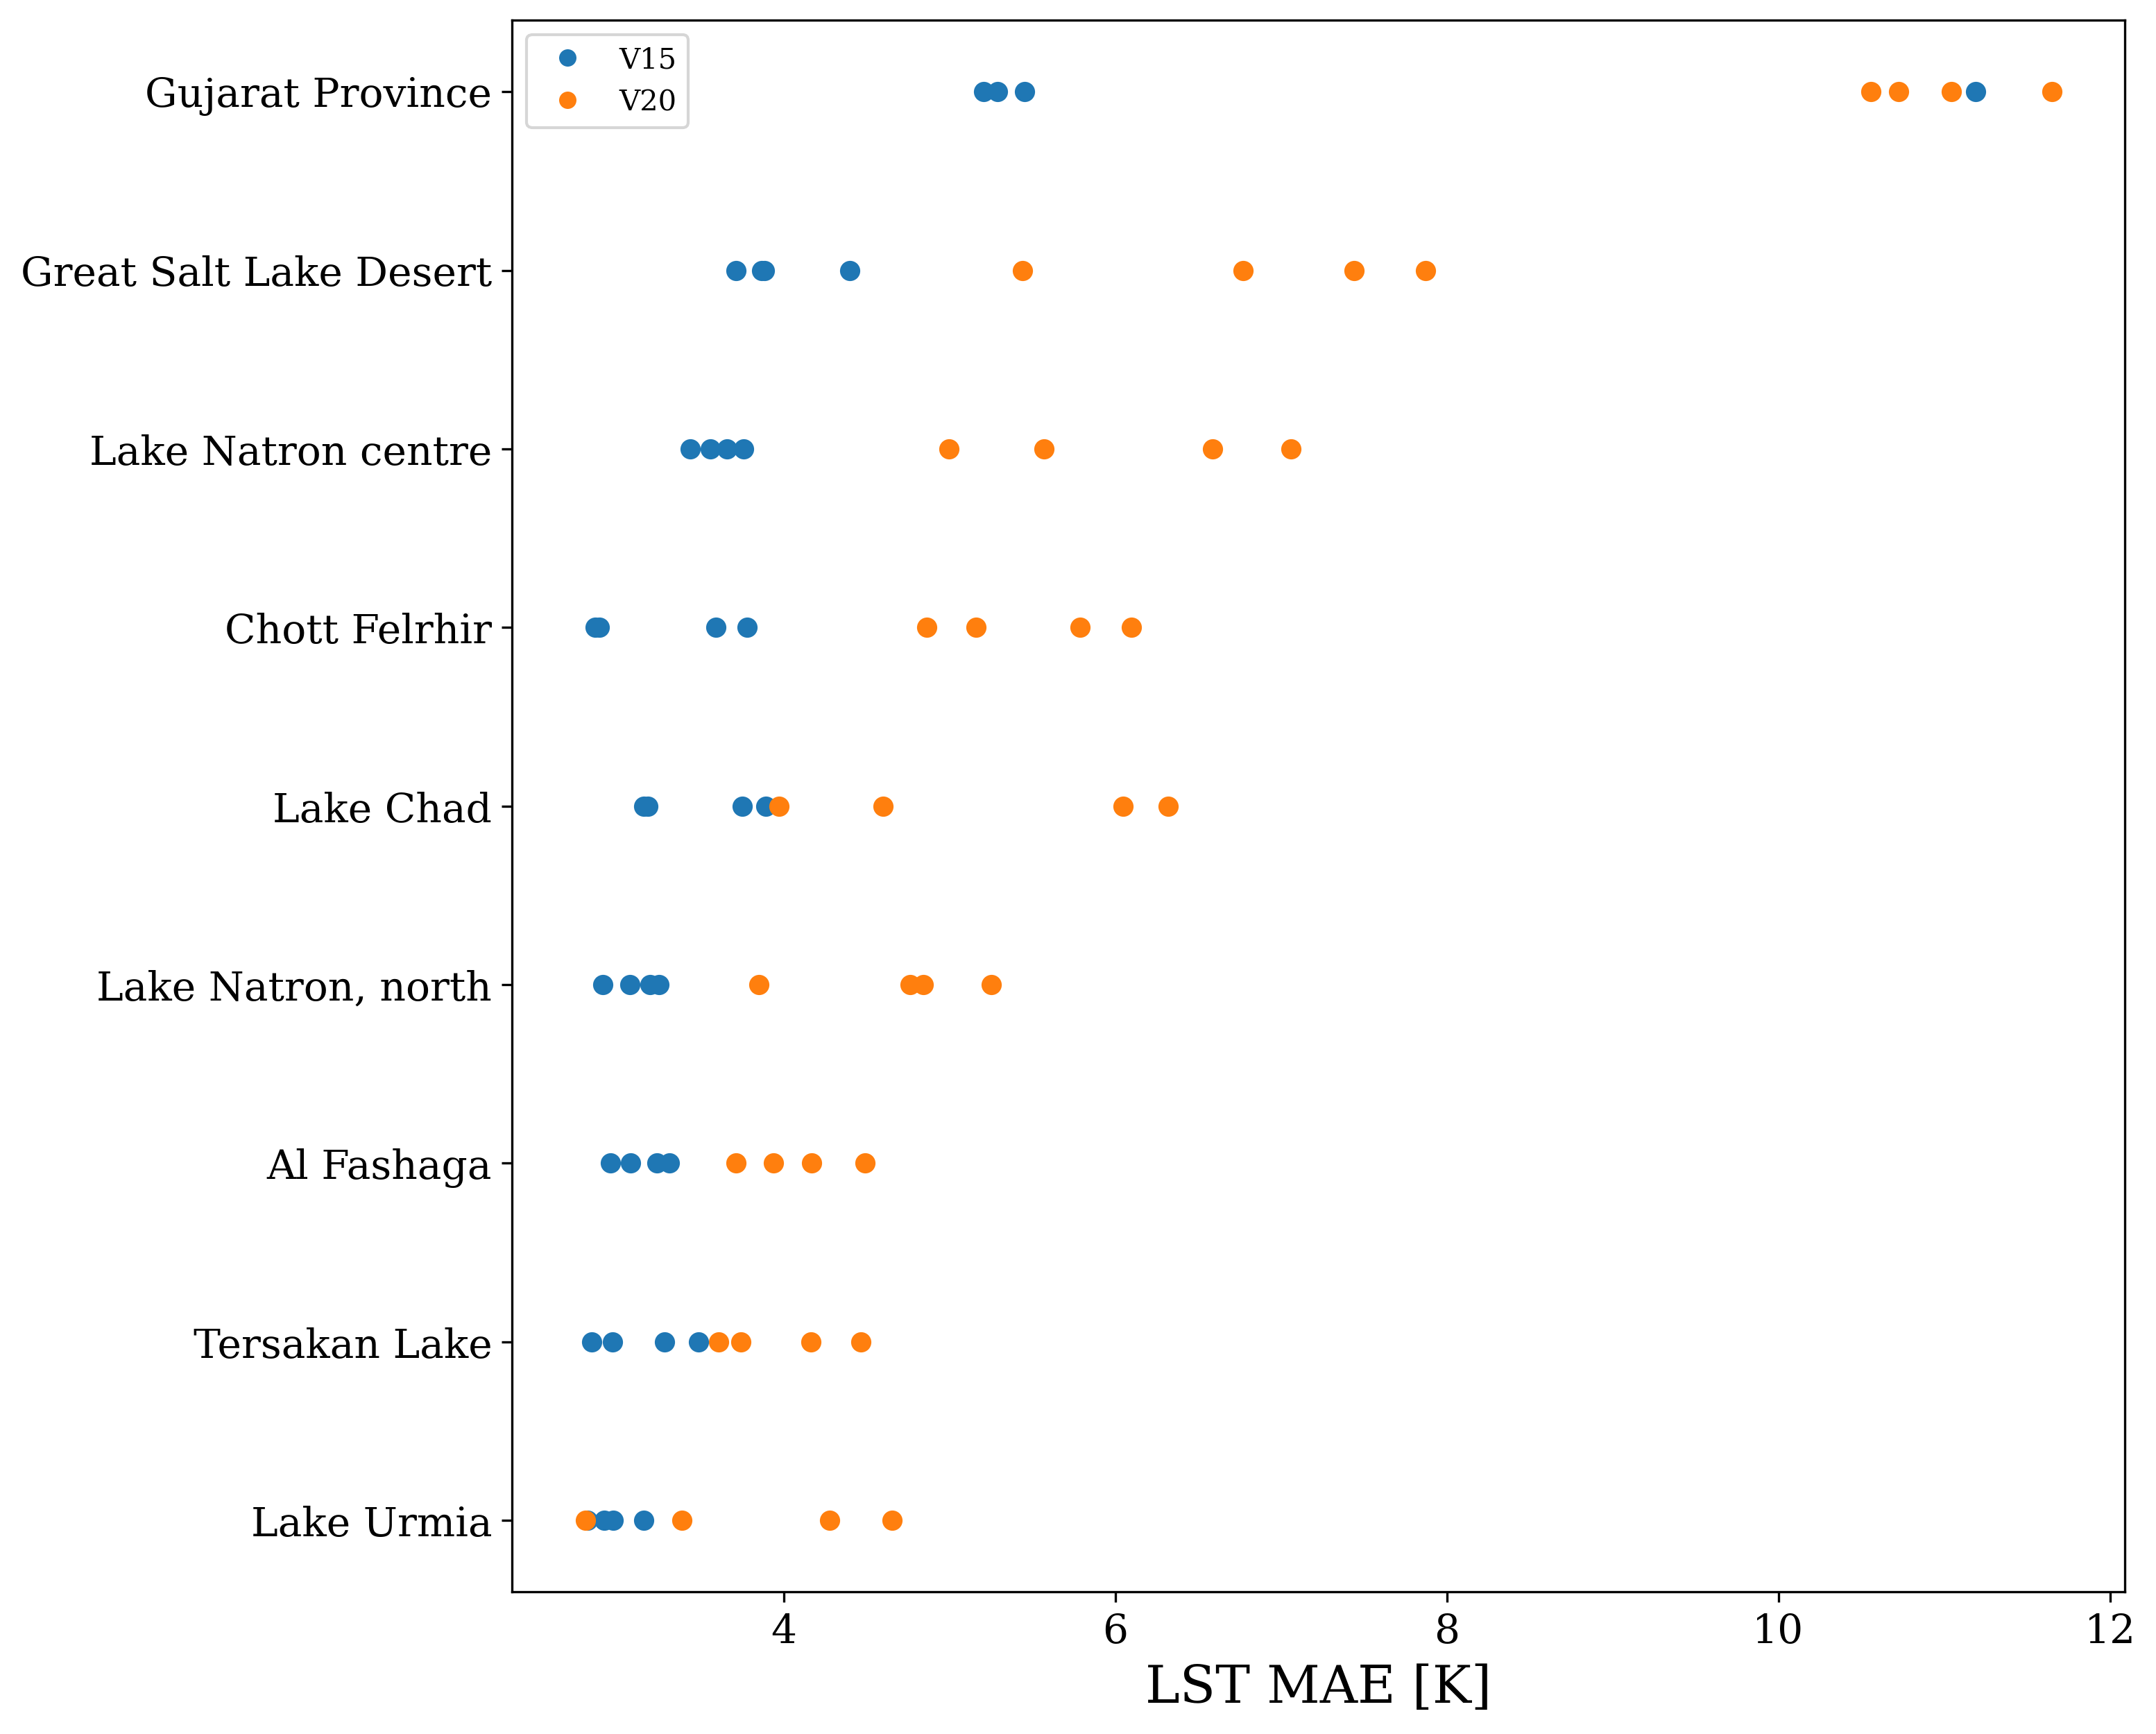
\includegraphics[width=\columnwidth]{selected_points_shift_plot_new}
	\caption{\DIFaddFL{As Fig. \ref{fig:global_shift_plot} for selected locations in the lakes grid point category where the added V20 data results in worse predictions when compared to V15.}} 
	\label{fig:lake_sub_categories}
\end{figure}


\DIFaddend \subsubsection{Category: Vegetation Updates}
\DIFdelbegin %DIFDELCMD < \label{V20Vegetation}
%DIFDELCMD < 	%%%
\DIFdel{Whilst the edits to the V15 lake fields generally act to increase the prediction accuracy, indicating that these fields are accurate and informative, changes to the vegetation generally give worse predictions.We can see from from Table \ref{tab:V1520_results} that the mean prediction accuracywhen using the updated fields decreases by 0.49K over 58 points . For all points apart from one, the }\textit{\DIFdel{cvh}} %DIFAUXCMD
\DIFdelend \DIFaddbegin \DIFadd{The Vegetation updates category, restricts analysis to grid points with significant change to high vegetation cover, where  the high vegetation cover is substituted with either low vegetation or bare ground, and vice versa. For this category the prediction accuracy of V20 decreased globally (over 58 grid-cells only) on average by 0.04K. However, this shift is much smaller than the training noise between successive VESPER iterations ($\sigma_{\rm V15} = 0.04$, $\sigma_{\rm V20} = 0.15$) and so it is hard to make definitive statements about the performance of the updated vegetation physiographic fields as a whole (see e.g. Fig \ref{fig:veg-noise}). The best we can say is that the updated V20 vegetation fields offer no global improvement in the LST prediction accuracy. }\newline 

\DIFadd{If we isolate our analysis to individual grid points where the training noise is small (highlighted by $*$ points in Fig \ref{fig:veg-noise}) we can discern that there are multiple locations where the high vegetation }\DIFaddend fraction was decreased \DIFdelbegin \DIFdel{, }\DIFdelend \DIFaddbegin \DIFadd{(}\DIFaddend often quite drastically to zero\DIFdelbegin \DIFdel{, i.e. }\DIFdelend \DIFaddbegin \DIFadd{), }\DIFaddend specifying that there should just be bare ground\DIFdelbegin \DIFdel{in these grid boxes. Whilst this may be accurate for some points, by inspecting }\DIFdelend \DIFaddbegin \DIFadd{, but thorough inspection of }\DIFaddend these areas with satellite imagery \DIFdelbegin \DIFdel{it is clear that there are regions which are in fact areas of }\DIFdelend \DIFaddbegin \DIFadd{revealed that they should in fact be covered with }\DIFaddend high vegetation (\DIFaddbegin \DIFadd{see }\DIFaddend e.g. \DIFdelbegin \DIFdel{Fig }\DIFdelend \DIFaddbegin \DIFadd{Figure }\DIFaddend \ref{fig:cvh}) and that \DIFdelbegin \DIFdel{it is inaccurate to simply remove all vegetation from these grid boxes. It is also notable that the  grid pointswhich have the largest drop in predictive performance when going from V15 to }\DIFdelend \DIFaddbegin \DIFadd{updating the }\DIFaddend V20 \DIFdelbegin \DIFdel{are all grid points where the vegetation fraction is severely }\DIFdelend \DIFaddbegin \DIFadd{high vegetation cover was erroneous for these grid-cells. Moreover, for this subset of less noisy grid points, the strength of the drop in LST predictability in VESPER\_V20 comparing to VESPER\_V15 is approximately linearly dependent to the degree of reduction in high vegetation fraction, when the vegetation is replaced with bare ground (i.e. $\delta_{\rm V20}$ is maximally positive when the grid-cell that was fully covered with forest becomes fully covered with bare ground – high vegetation cover is }\DIFaddend reduced to zero\DIFdelbegin \DIFdel{. This suggests that such extreme changes may be strong over-corrections, and more modest updates to the vegetation fields may be more accurate. These erroneous }\DIFdelend \DIFaddbegin \DIFadd{). These erroneous grid-cells in }\DIFaddend V20 vegetation fields are likely \DIFdelbegin \DIFdel{inherited from  initial datasets used to update vegetation or }\DIFdelend \DIFaddbegin \DIFadd{to appear }\DIFaddend during the interpolation. The errors in these regions will in turn corrupt the LST predictions and mitigate the gain from a more accurate representation of the lake water. \DIFaddbegin \DIFadd{The majority of grid cells in this category (57/58) are modified in this way where the high vegetation fraction is severely reduced, however due to the large degree of training noise and the small number of points, it is difficult to draw any definitive conclusions for the category as a whole.
	}\DIFaddend \begin{figure}[h!]
	\subfloat[\label{fig:cvh1}]{\includegraphics[width=0.48\textwidth]{siberut_hr.jpg}} \\
	\subfloat[\label{fig:cvh2}]{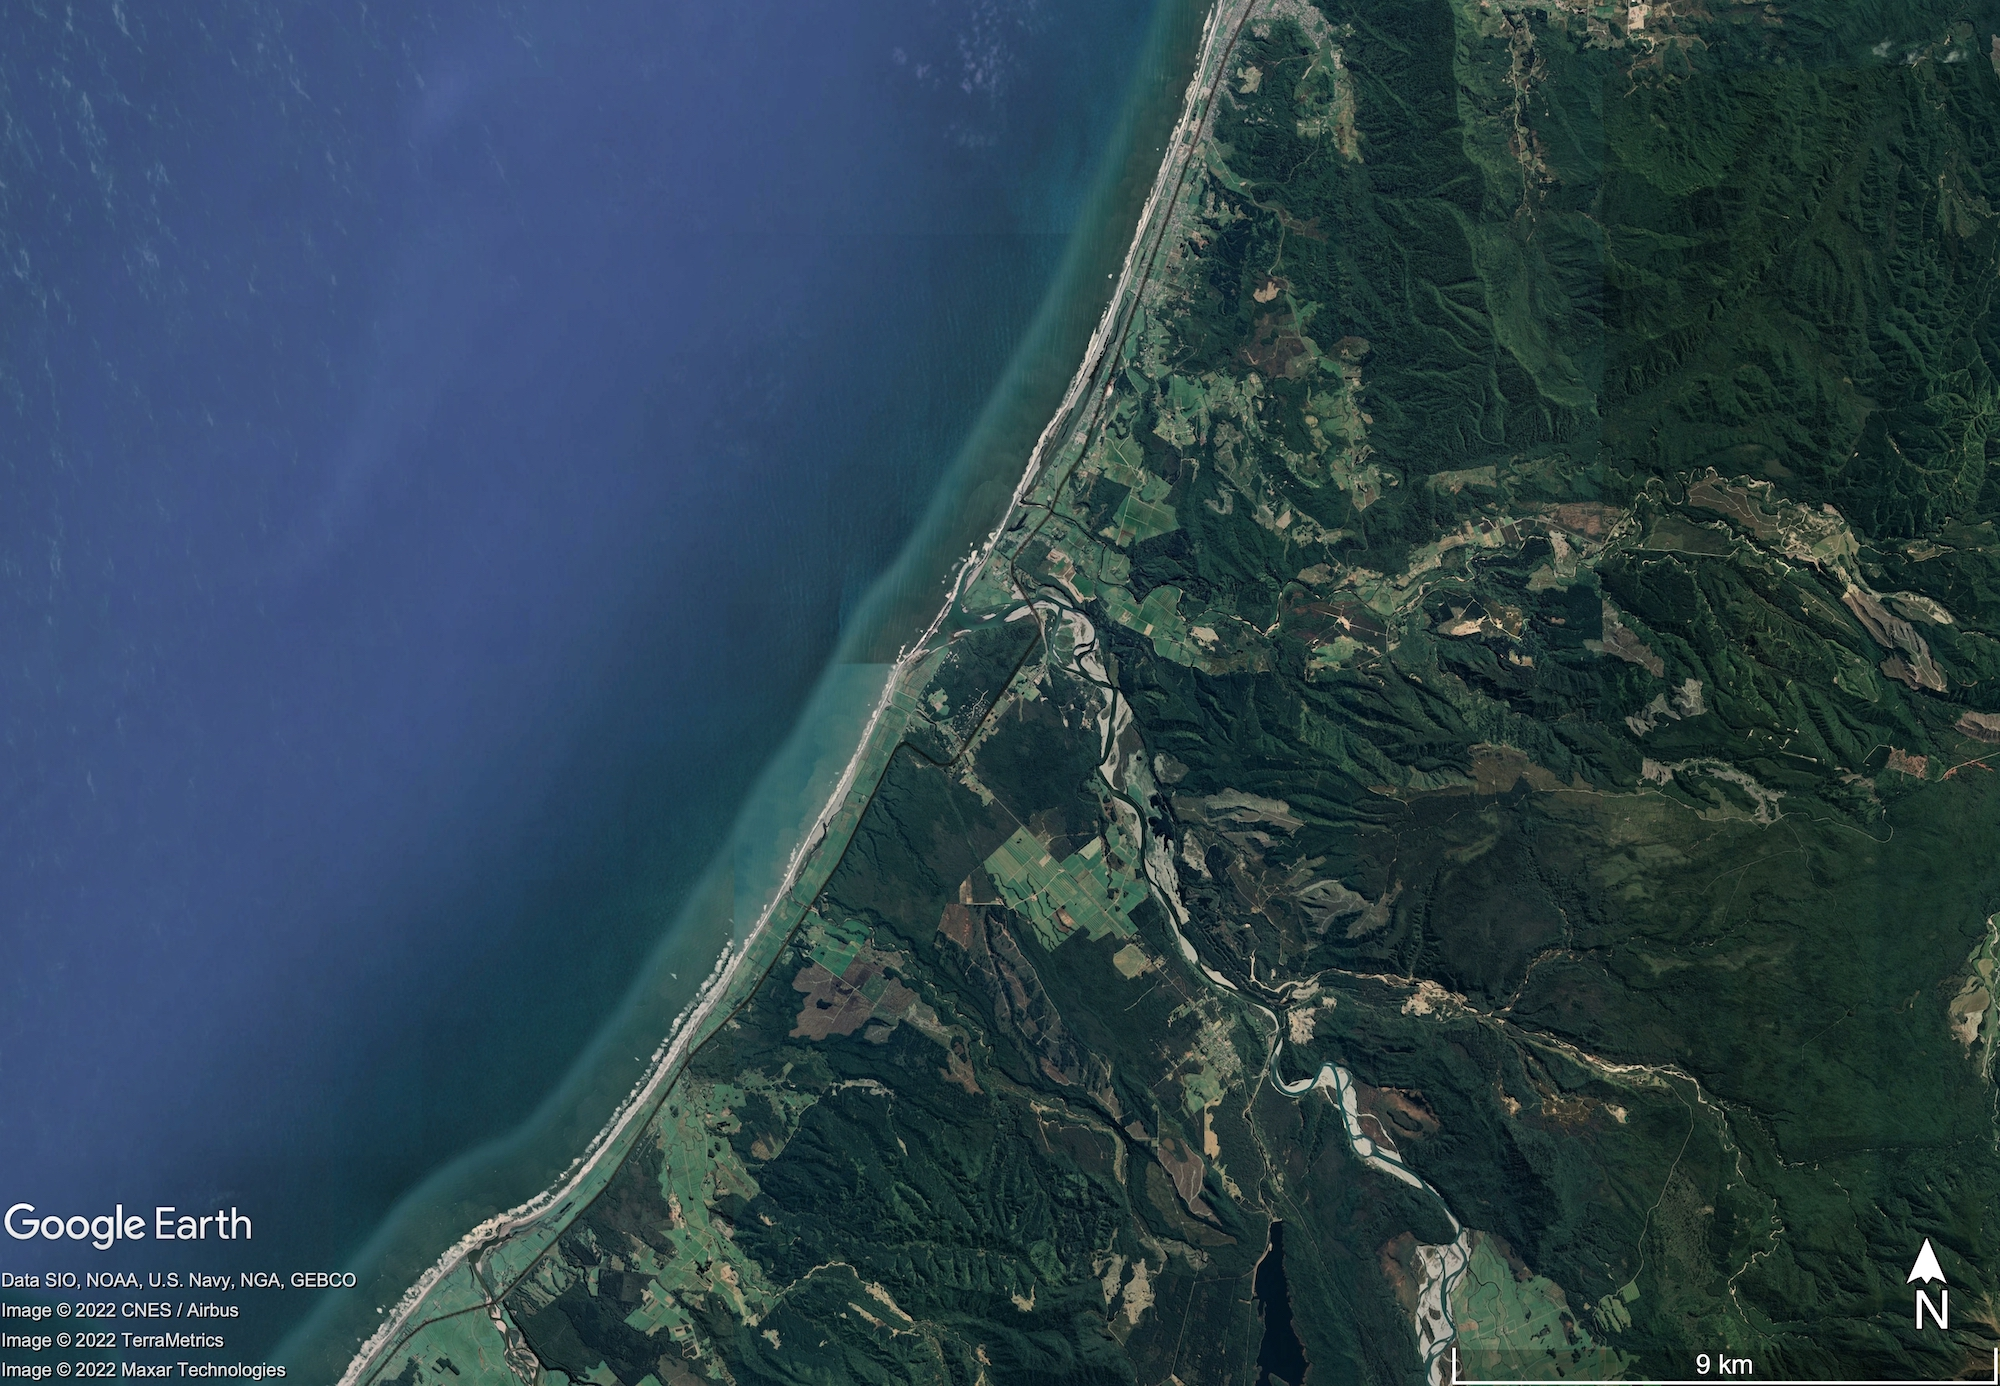
\includegraphics[width=0.48\textwidth]{NewZealandVeg.jpg}}
	\caption{Satellite imagery of \DIFdelbeginFL \DIFdelFL{grid boxes }\DIFdelendFL \DIFaddbeginFL \DIFaddFL{grid-cells }\DIFaddendFL in \DIFdelbeginFL \textit{\DIFdelFL{(a)}} %DIFAUXCMD
\DIFdelendFL \DIFaddbeginFL \DIFaddFL{(a) }\DIFaddendFL Siberut Island, Indonesia and \DIFdelbeginFL \textit{\DIFdelFL{(b)}} %DIFAUXCMD
\DIFdelendFL \DIFaddbeginFL \DIFaddFL{(b) }\DIFaddendFL South Island, New Zealand. For both \DIFdelbeginFL \DIFdelFL{points it is expected }\DIFdelendFL \DIFaddbeginFL \DIFaddFL{grid-cells }\DIFaddendFL according to the updated V20 \DIFdelbeginFL \DIFdelFL{fields that }\DIFdelendFL \DIFaddbeginFL \DIFaddFL{field set }\DIFaddendFL there \DIFdelbeginFL \DIFdelFL{is }\DIFdelendFL \DIFaddbeginFL \DIFaddFL{should be }\DIFaddendFL no vegetation, just bare ground. VESPER \DIFdelbeginFL \DIFdelFL{can identify }\DIFdelendFL \DIFaddbeginFL \DIFaddFL{identified }\DIFaddendFL these \DIFdelbeginFL \DIFdelFL{erroneous }\DIFdelendFL \DIFaddbeginFL \DIFaddFL{erroneously }\DIFaddendFL updated \DIFdelbeginFL \DIFdelFL{fields}\DIFdelendFL \DIFaddbeginFL \DIFaddFL{areas}\DIFaddendFL .} 
	\label{fig:cvh}
\end{figure}

\DIFaddbegin \begin{figure}
	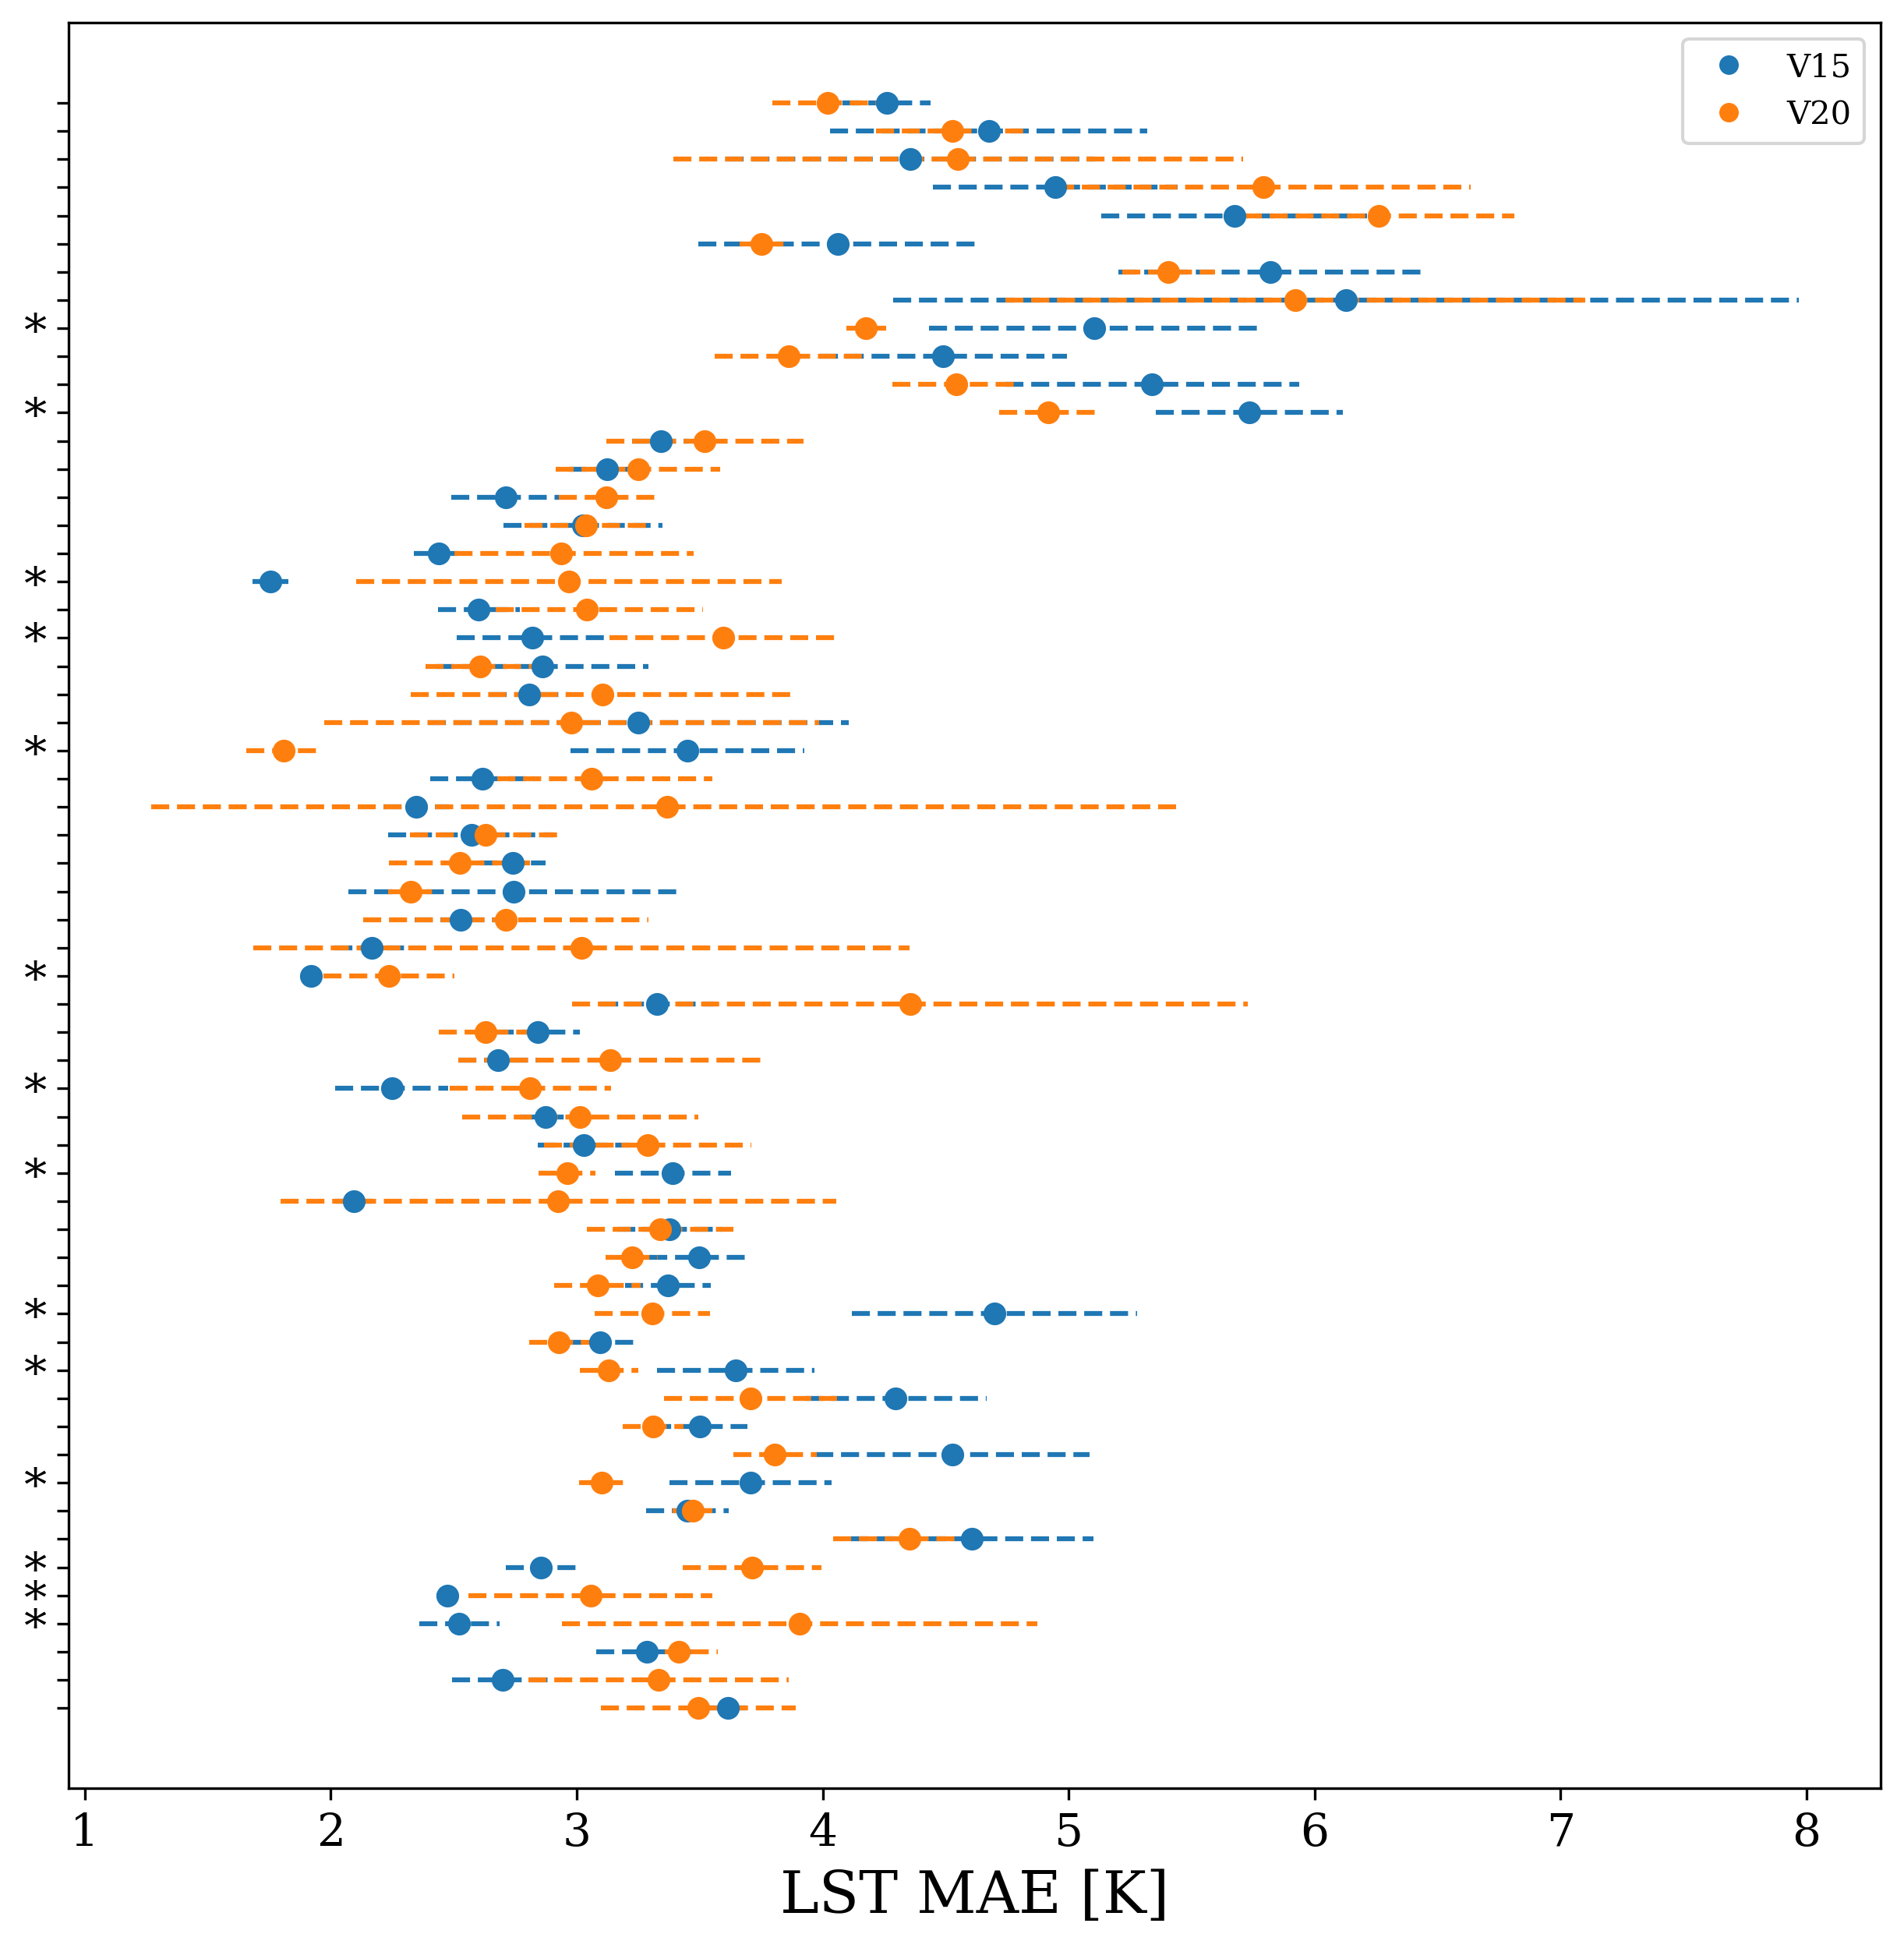
\includegraphics[width=\columnwidth]{veg_plot_noise}
	\caption{\DIFaddFL{Distribution of prediction errors in the LST, for VESPER\_V15 and VESPER\_V20, for all 58 grid points in the vegetation category. There is evidently a large degree of noise, with predictions from both generations of VESPER model highly overlapping. Points with reduced training noise are highlighted with a $*$.}}
	\label{fig:veg-noise}
\end{figure}


\DIFaddend \subsubsection{Category: Glacier Updates}\DIFdelbegin %DIFDELCMD < \label{V20Glacier}
%DIFDELCMD < 	%%%
\DIFdel{The }\DIFdelend \DIFaddbegin \label{sec:glacier}
\DIFadd{The Glacier Updates category in general shows improvement in LST predictability in VESPER\_}\DIFaddend V20 \DIFdelbegin \DIFdel{updates to the glacier fraction also generally improve the predictions, with a mean $\delta_{\rm V20} = -0.14$ K }\DIFdelend \DIFaddbegin \DIFadd{comparing to VESPER\_V15 (see  Table  \ref{tab:categorisation})  –  prediction  accuracy  increases  globally  (}\DIFaddend over  1057  \DIFdelbegin \DIFdel{grid points. These improvements are concentrated }\DIFdelend \DIFaddbegin \DIFadd{grid-cells)  on  average  by  0.22K  ($\sigma_{\rm V15} = 0.03$, $\sigma_{\rm V20} = 0.02$), most notably }\DIFaddend around the Himalayas, the land either side of the Davis strait, as well as British Columbia and the Alaskan Gulf. Analogous to the Lakes Updates category whilst the introduction of the V20 \DIFdelbegin \DIFdel{fields generally improves the model, there are some selected regions }\DIFdelend \DIFaddbegin \DIFadd{glacier cover generally improves LST predictions, there is a small selection of grid points }\DIFaddend where the prediction gets worse. These are heavily concentrated  in  the  southern  hemisphere,  in  particular  on  the  \DIFdelbegin \DIFdel{south western }\DIFdelend \DIFaddbegin \DIFadd{south-western  }\DIFaddend edge  of  South  America  and  the  South Shetland Islands \DIFdelbegin \DIFdel{- }\DIFdelend \DIFaddbegin \DIFadd{(}\DIFaddend which lie closer to Antarctica\DIFdelbegin \DIFdel{- as well as }\DIFdelend \DIFaddbegin \DIFadd{), and }\DIFaddend some parts of the Himalayas. This \DIFdelbegin \DIFdel{deficit }\DIFdelend \DIFaddbegin \DIFadd{deterioration }\DIFaddend in performance in these areas is not due to erroneous \DIFdelbegin \DIFdel{updated }\DIFdelend \DIFaddbegin \DIFadd{update of }\DIFaddend V20 \DIFdelbegin \DIFdel{fields, but instead is a data quality issue whereby we do not have a lot of MODIS observations in these areas which have a large degree or orography and cloud cover.This can be seen in Fig \ref{fig:MODIS_obs} for the above mentioned regions. Consequently the neural net model }\DIFdelend \DIFaddbegin \DIFadd{glacier cover, but related to the Aqua-MODIS data (i.e. sparse availability due to clouds, and less certain due to orography, see Figure \ref{fig:modis_plot_1}). Consequently, VESPER }\DIFaddend finds it difficult to make accurate predictions in this region \DIFdelbegin \DIFdel{, and this iteration of the model has settled into a local minimum for V20 which is worse than }\DIFdelend \DIFaddbegin \DIFadd{and for these points there is often a large degree of training noise, with considerable overlap between VESPER\_}\DIFaddend V15 \DIFdelbegin \DIFdel{in these areas. If we isolate just grid points where we have a large number of observations (we take }\DIFdelend \DIFaddbegin \DIFadd{and VESPER\_V20. If grid- cells with scarce amount of Aqua-MODIS observations (i.e. }\DIFaddend mean number of \DIFdelbegin \DIFdel{MODIS  observations per ERA data point $> 50$) }\DIFdelend \DIFaddbegin \DIFadd{Aqua-MODIS observations per day over the year per ERA5 grid-cell is >50) are removed from the analysis }\DIFaddend then the worst performing \DIFdelbegin \DIFdel{grid points are excluded. In this case there do remain }\DIFdelend \DIFaddbegin \DIFadd{grid-cells become excluded, yet }\DIFaddend a few areas where \DIFdelbegin \DIFdel{the }\DIFdelend \DIFaddbegin \DIFadd{VESPER\_}\DIFaddend V20 \DIFdelbegin \DIFdel{model underperforms with respect to }\DIFdelend \DIFaddbegin \DIFadd{underperforms VESPER\_}\DIFaddend V15 \DIFaddbegin \DIFadd{remain}\DIFaddend . For  example\DIFaddbegin \DIFadd{, }\DIFaddend there is a \DIFdelbegin \DIFdel{grid point in the Alaskan gulf on the Bering Glacierwith $\delta_{\rm V20} = +2.16$ K. This point }\DIFdelend \DIFaddbegin \DIFadd{grid-cell in Chilean Patagonia that contains the Calluqueo Glacier, close to Monte San Lorenzo where $\delta_{\rm V20} = 2.49$ ($\sigma_{\rm V15} = 0.38$, $\sigma_{\rm V20} = 0.62$). This grid-cell }\DIFaddend has been updated in V20 \DIFdelbegin \DIFdel{to have a higher glacier proportion (0.68 to 0.92), such that the grid box should be almost completely dominated by ice. Nearly all low vegetation was also completely removed (}\textit{\DIFdel{cvl}} %DIFAUXCMD
\DIFdel{from 0.10 to 0.007) and the lake depth increased from $\sim 2$m to $\sim$27, in conjunction with a modest decrease in the lake fraction, from 0.07 to 0.01. Satellite imagery of the region (Fig. \ref{fig:glacier}) shows an area that does have a significant ice fraction , but perhaps not as great as $\gtrsim 90 \%$, suggesting that the V20 updates }\DIFdelend \DIFaddbegin \DIFadd{field set comparing to V15 by strongly increasing glacier cover from 0.0 to 0.44), decreasing low vegetation cover (from 0.22 to 0.12) and high vegetation cover (from 0.16 to 0.09) as well as modestly decreasing lake cover (from 0.02 to 0.007). According to satellite imagery (see Figure \ref{fig:glacier1}) the glacier only occupies a small fraction of the overall grid-cell, and the updated glacier cover }\DIFaddend may have been an over correction. \DIFdelbegin \DIFdel{The Bering glacier is also known to be a time variable region which varies in size over the course of the season, whilst on longer timescales exhibits a general retreat of the terminus over time, coupled with periodic surges in the glacier flow around every 20 years \mbox{%DIFAUXCMD
\cite{Bering2010}}\hskip0pt%DIFAUXCMD
.It is therefore a complex region not necessarily well represented by a static fractional field. There also appears to be some low level vegetation present, and again removing all vegetation for this region may have been an overcorrection. Another notable grid }\DIFdelend \DIFaddbegin \DIFadd{Moreover, this is an complex orographic area with snowy mountain peaks at high altitude and deep valleys, therefore the temperature response due to the glacier feature could be atypical compared to e.g. the Alaskan Gulf or the Davis straight. There is also substantial vegetation cover in the valleys that may not be being properly described. A similar }\DIFaddend point is in the  Chilean Andes \DIFaddbegin \DIFadd{(see Figure \ref{fig:glacier2})}\DIFaddend ,  by the Juncal Glacier \DIFdelbegin \DIFdel{. Here the ice fraction was increased in }\DIFdelend \DIFaddbegin \DIFadd{with $\delta_{\rm V20} = 1.26$ ($\sigma_{\rm V15} = 0.68$, $\sigma_{\rm V20} = 0.29$). Here }\DIFaddend V20 \DIFaddbegin \DIFadd{glacier cover was increased }\DIFaddend to 0.25 \DIFdelbegin \DIFdel{from zero }\DIFdelend \DIFaddbegin \DIFadd{compared to 0.00 }\DIFaddend in V15\DIFdelbegin \DIFdel{, an attempt to better represent the glacial ice. However, $\delta_{\rm V20} = +2.67$K. In fact, the glacier itself only occupies }\DIFdelend \DIFaddbegin \DIFadd{. Again, this is may have been an over correction, as the glacier constitutes only }\DIFaddend a  small fraction of the \DIFdelbegin \DIFdel{overall grid box, and the updated field may have been an over correction. Moreover, this is }\DIFdelend \DIFaddbegin \DIFadd{grid cell. As with the Calluqueo Glacier this is also }\DIFaddend an area with lots of orography \DIFdelbegin \DIFdel{, with snowy mountains at high altitude and deep valleys. Therefore the temperature response due to the glacier feature could be atypical compared to e. g. the Alaskan Gulf or the Davis straight. For both these points we can again see how VESPER 's ability to identify grid points where the model predictions become worse in this way is a powerful tool for identifying updated fieldsor regions which are insufficiently accurate or informative. 
	}%DIFDELCMD < \newline 
%DIFDELCMD < 	%%%
\DIFdelend \DIFaddbegin \DIFadd{and so could have an atypical temperature response. For both of these points VESPER managed  to identify potential inaccuracies in updated glacier cover, and once again proved itself as a useful tool for quality control of surface physiographic fields. 
	}\DIFaddend \begin{figure}[h!]
	\DIFdelbeginFL %DIFDELCMD < \subfloat[\label{fig:glacier1}]{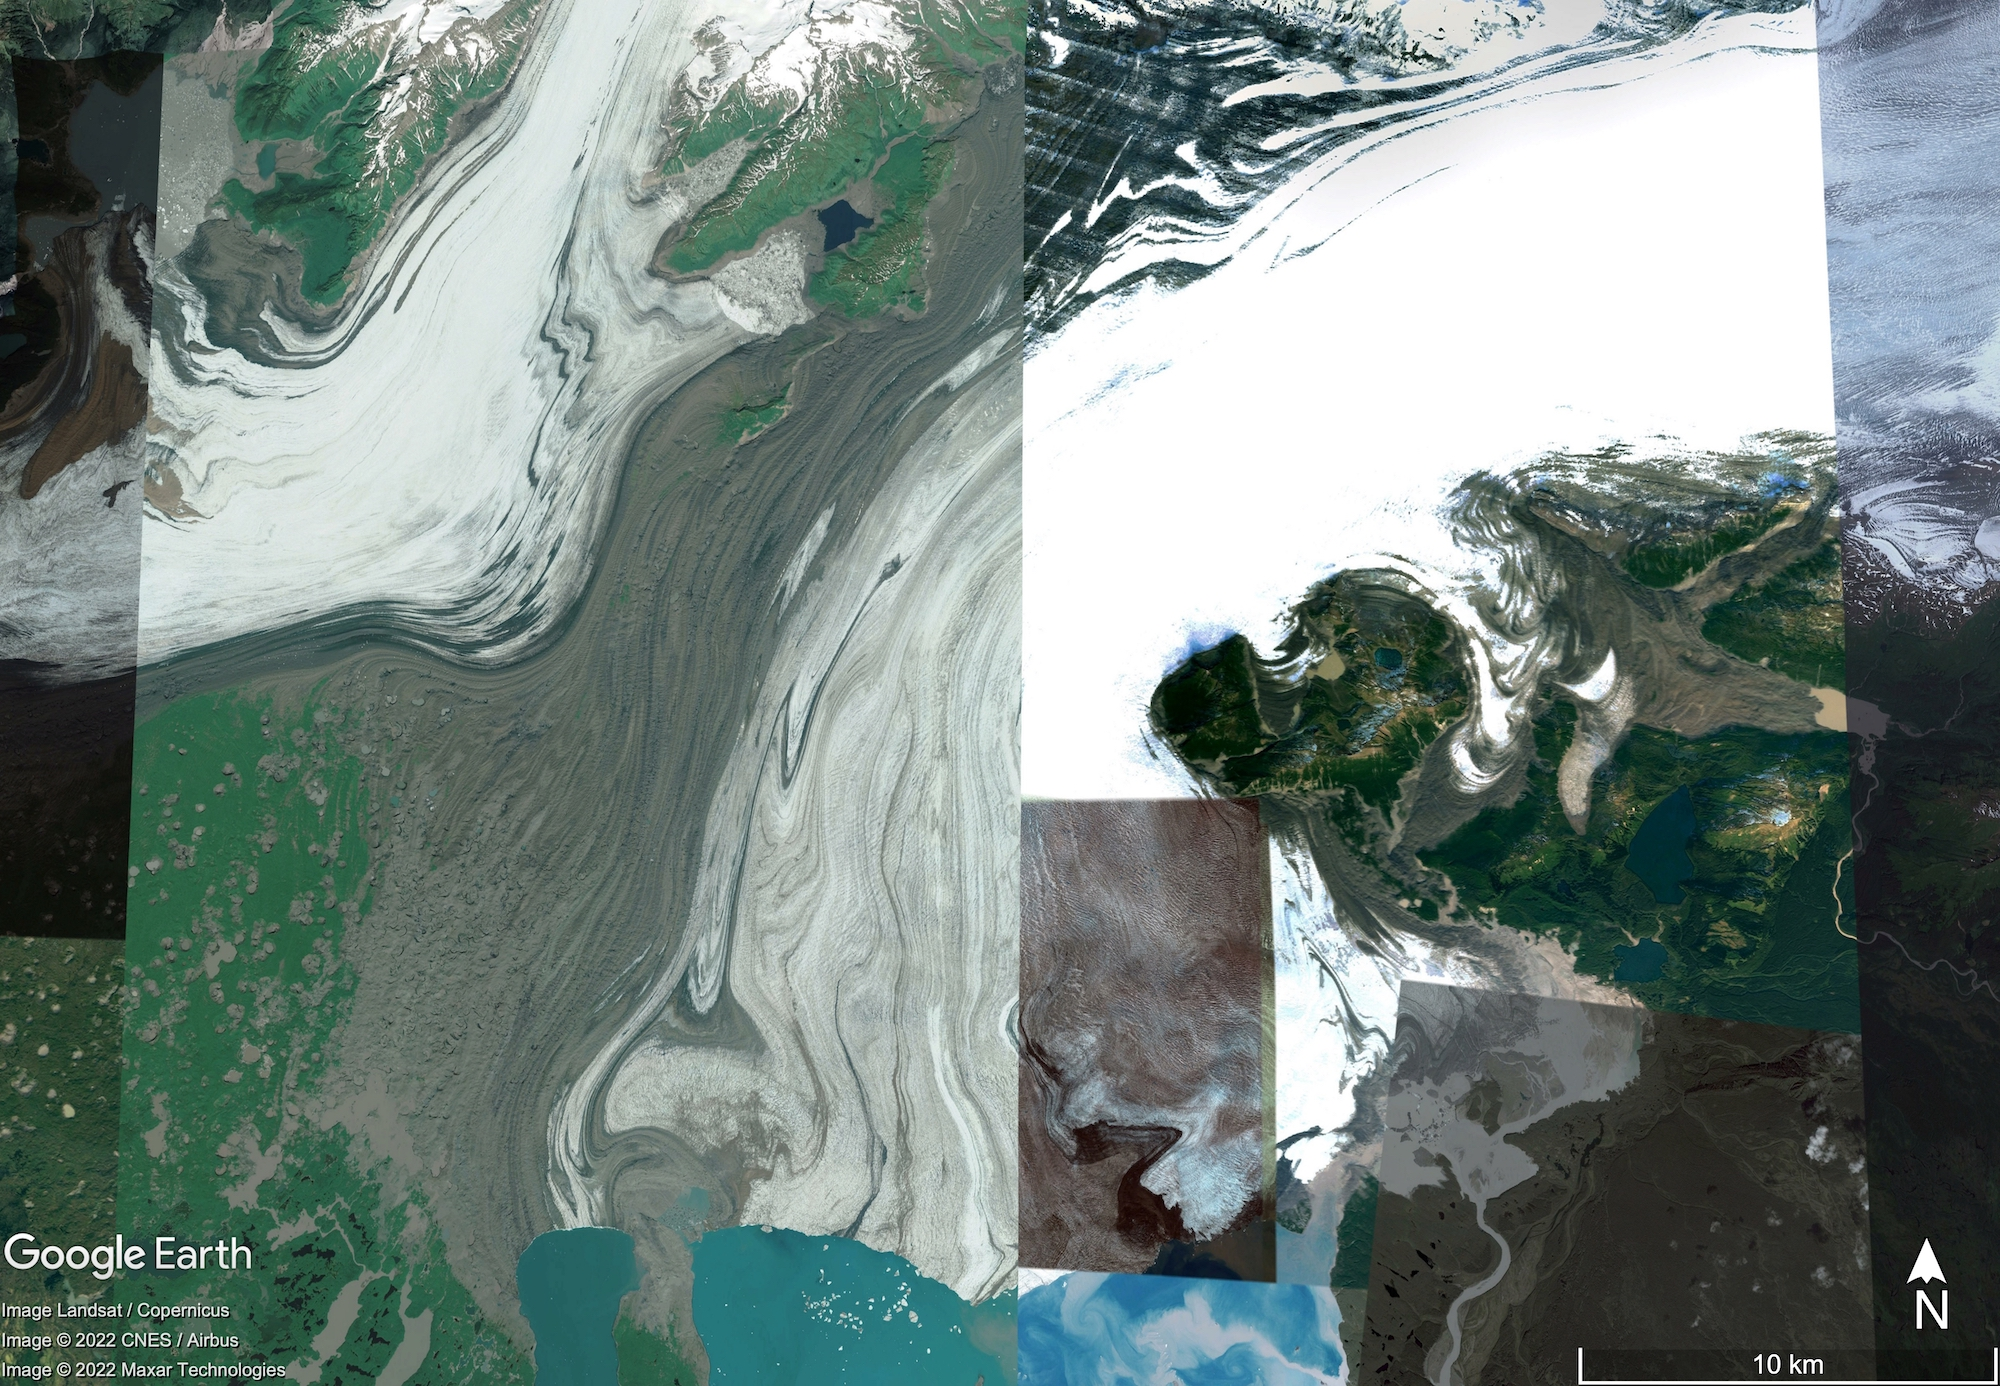
\includegraphics[width=0.48\textwidth]{Alaska4.jpg}} %%%
\DIFdelendFL \DIFaddbeginFL \subfloat[\label{fig:glacier1}]{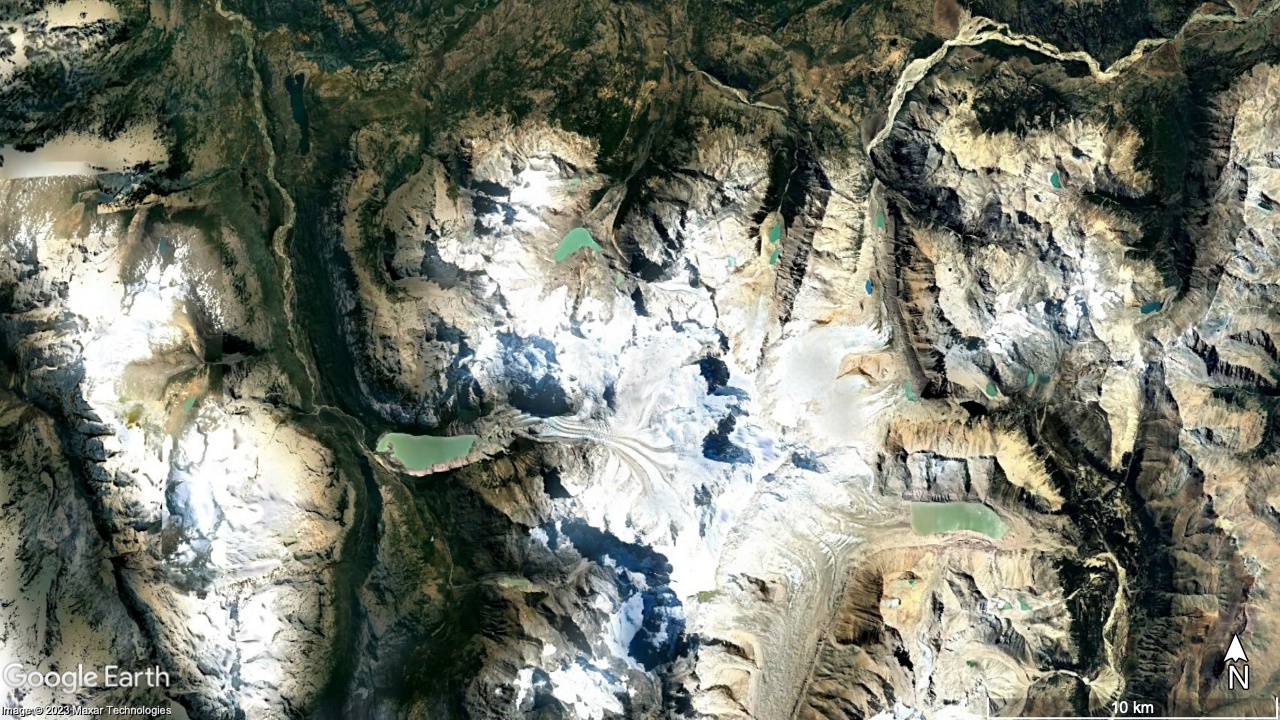
\includegraphics[width=0.48\textwidth]{pataginia2}} \DIFaddendFL \\
	\subfloat[\label{fig:glacier2}]{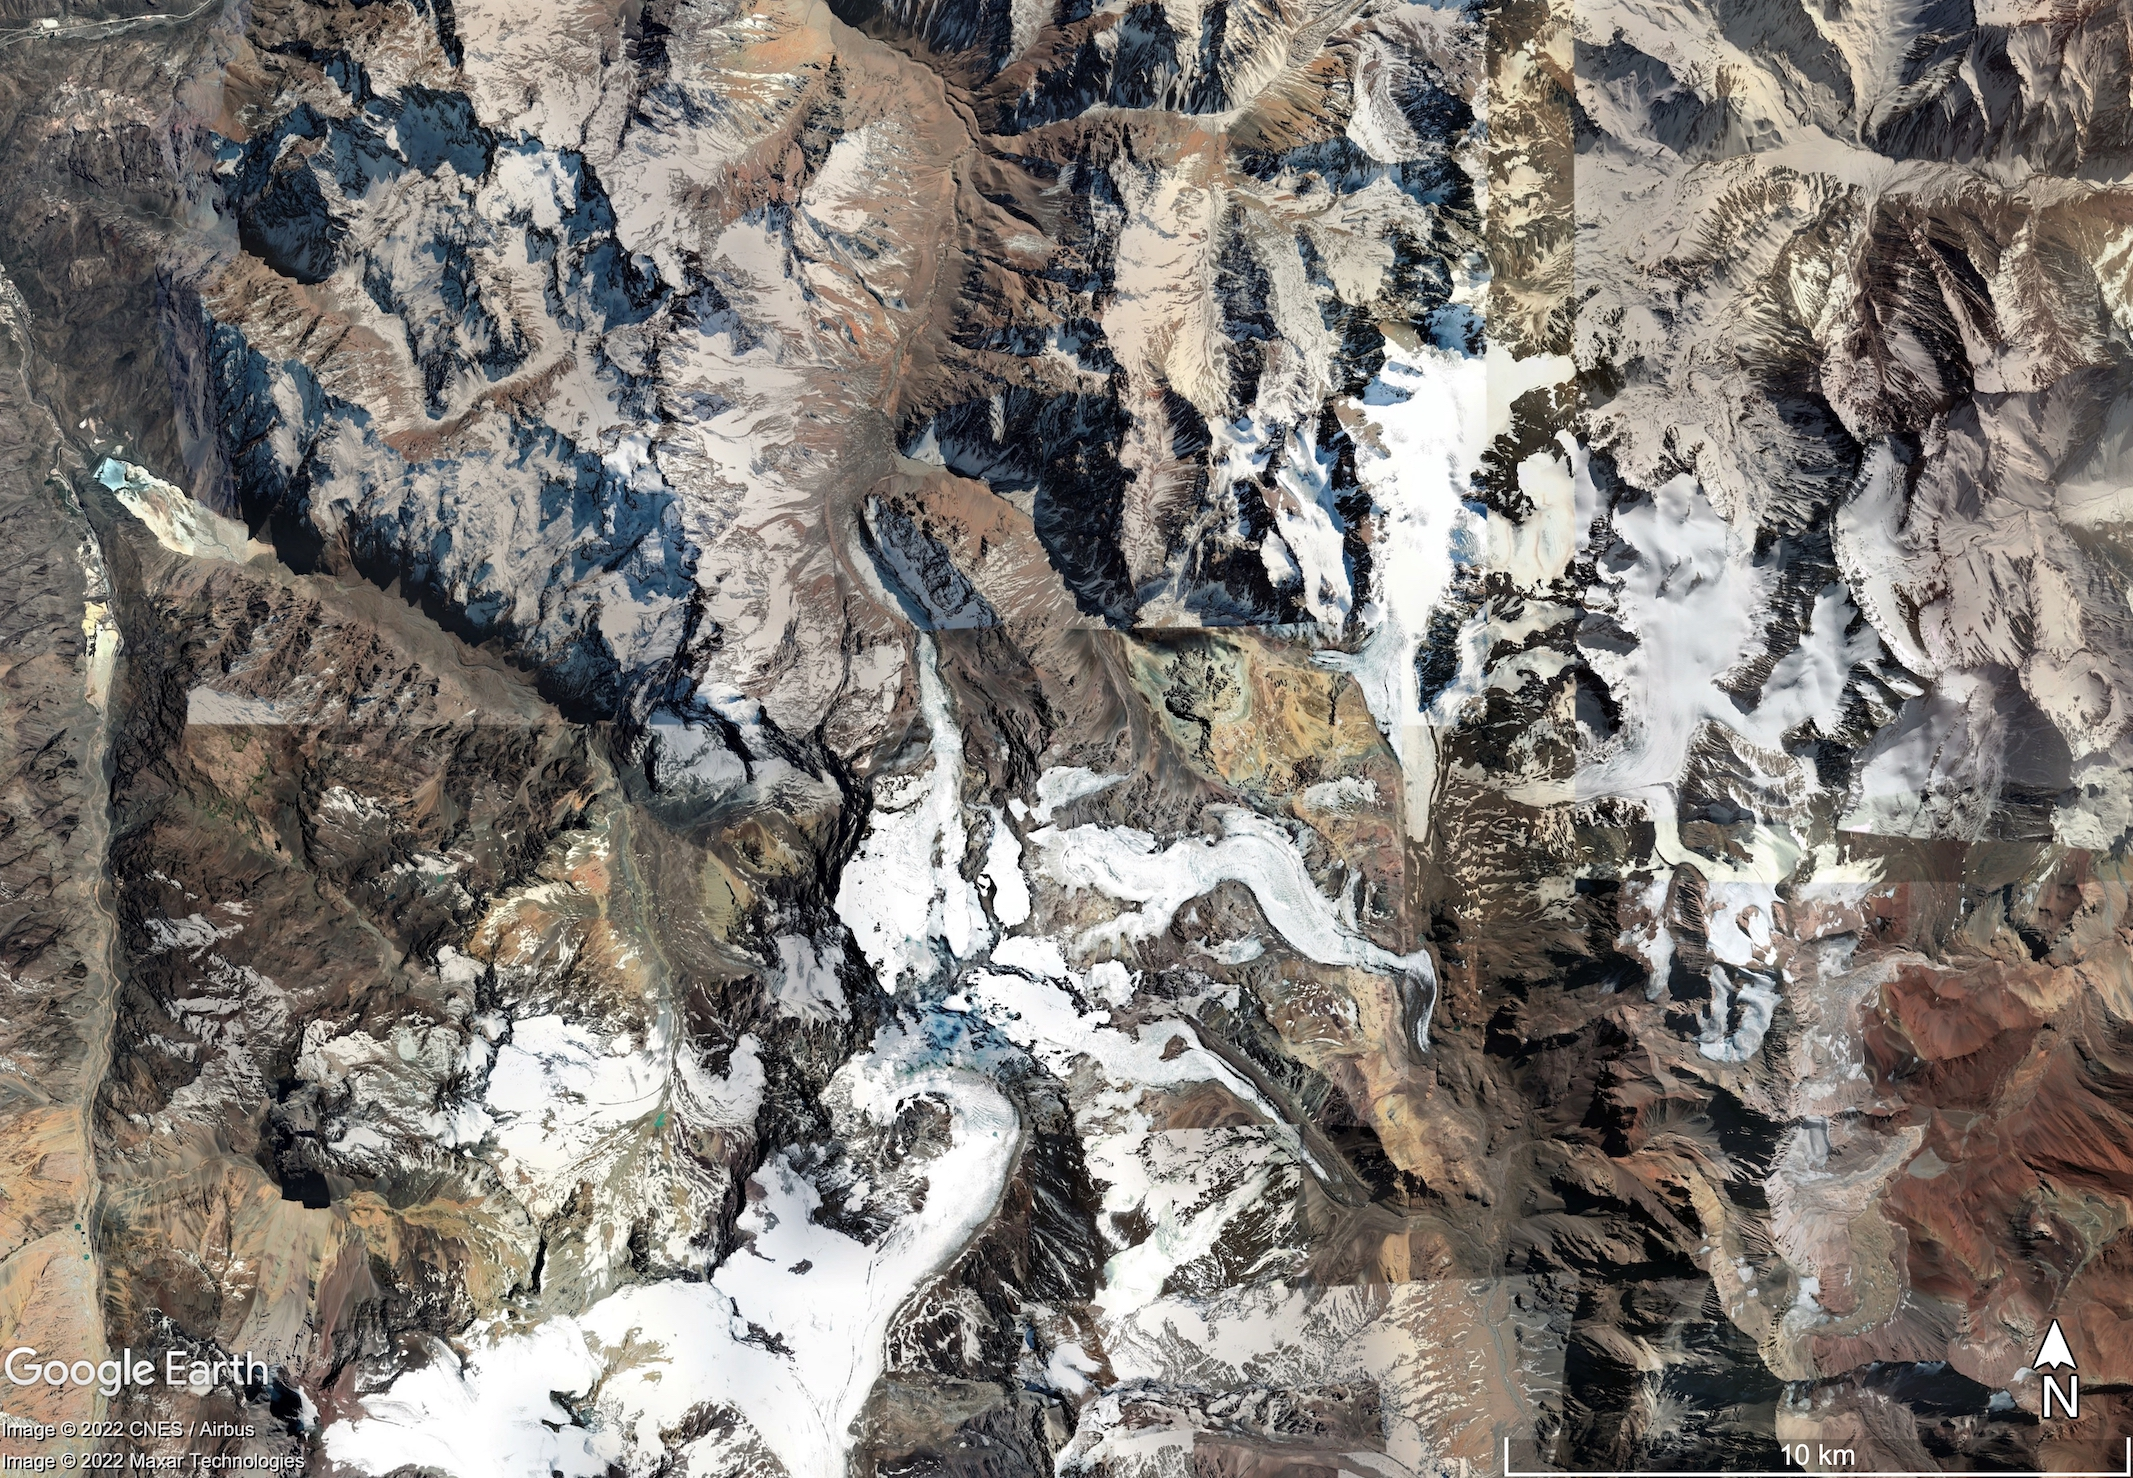
\includegraphics[width=0.48\textwidth]{Andes1.jpg}} 
	\caption{Satellite imagery of \DIFdelbeginFL \textit{\DIFdelFL{(a)}} %DIFAUXCMD
\DIFdelFL{Bering }\DIFdelendFL \DIFaddbeginFL \DIFaddFL{(a) Calluqueo }\DIFaddendFL Glacier, \DIFdelbeginFL \DIFdelFL{Alaskan Gulf}\DIFdelendFL \DIFaddbeginFL \DIFaddFL{Patagonia}\DIFaddendFL , and \DIFdelbeginFL \textit{\DIFdelFL{(b)}} %DIFAUXCMD
\DIFdelendFL \DIFaddbeginFL \DIFaddFL{(b) }\DIFaddendFL Juncal Glacier, Chile. \DIFdelbeginFL \DIFdelFL{For }\textit{\DIFdelFL{(a)}} %DIFAUXCMD
\DIFdelFL{it is expected that there is no vegetation and }\DIFdelendFL \DIFaddbeginFL \DIFaddFL{In }\DIFaddendFL the \DIFdelbeginFL \DIFdelFL{grid box to be primarily ($\gtrsim 90 \%$) dominated by ice. For }\textit{\DIFdelFL{(b)}} %DIFAUXCMD
\DIFdelFL{the }\DIFdelendFL updated V20 \DIFdelbeginFL \DIFdelFL{fields specify a $\gtrsim 25 \%$  glacier fraction. Evidently}\DIFdelendFL \DIFaddbeginFL \DIFaddFL{field set}\DIFaddendFL , the \DIFdelbeginFL \DIFdelFL{V20 fields }\DIFdelendFL \DIFaddbeginFL \DIFaddFL{assumption }\DIFaddendFL for \DIFaddbeginFL \DIFaddFL{region (a) is almost half ice cover with little vegetation, for region (b) is quarter covered with glacier; }\DIFaddendFL these \DIFdelbeginFL \DIFdelFL{grid boxes are }\DIFdelendFL \DIFaddbeginFL \DIFaddFL{assumptions seem to be }\DIFaddendFL insufficiently accurate or informative, as identified by VESPER.
	} 
	\label{fig:glacier}
\end{figure}

%DIF < \begin{figure}[h!]
	%DIF < 
	%DIF < 	\subfloat[\label{fig:cvh2}]{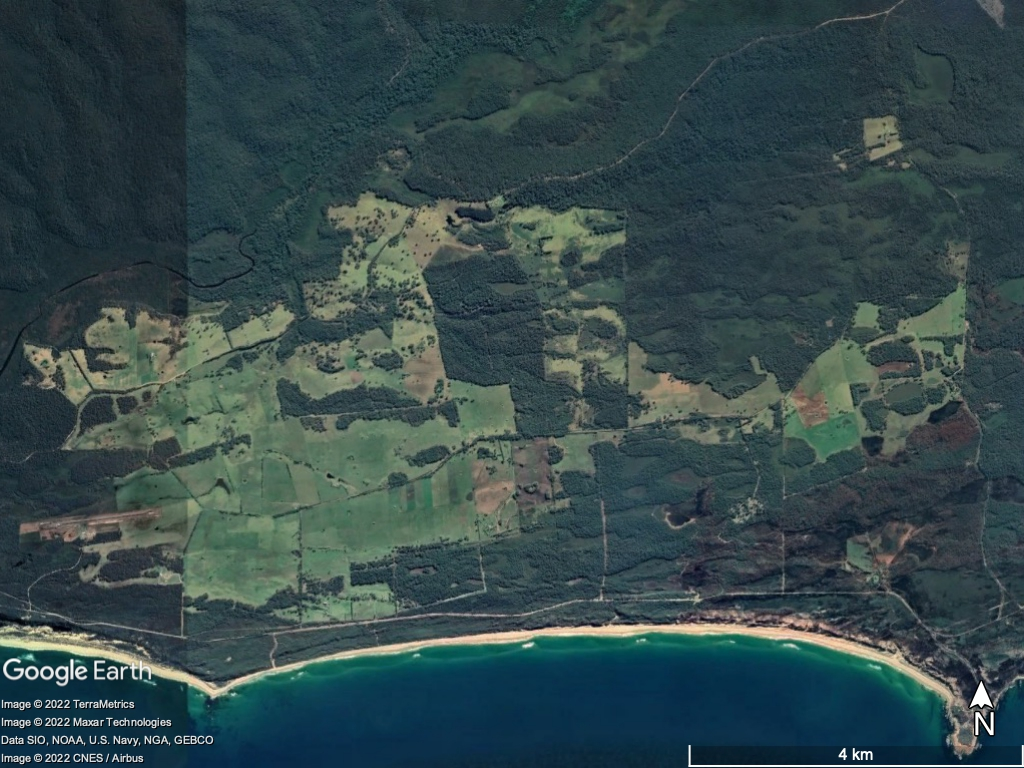
\includegraphics[width=0.48\textwidth]{australia_googleearth.jpg}} \\
	%DIF < 	\subfloat[\label{fig:cvh3}]{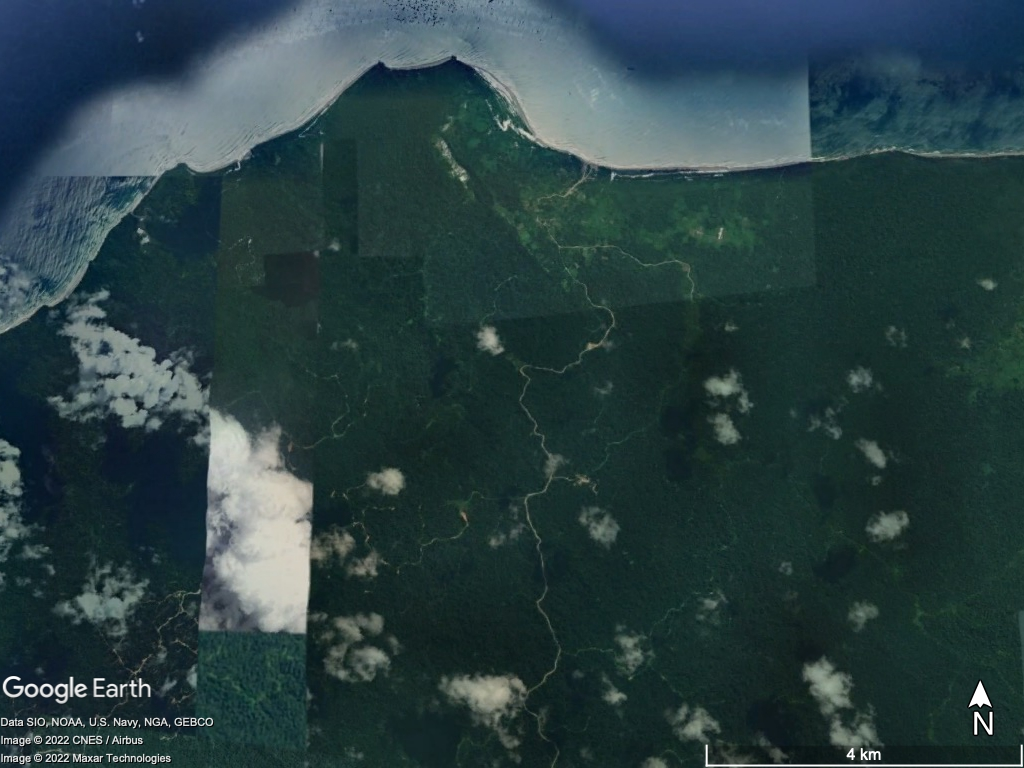
\includegraphics[width=0.48\textwidth]{cvh_hr.jpg}} \\
	%DIF < 	\subfloat[\label{fiig:cvh1}]{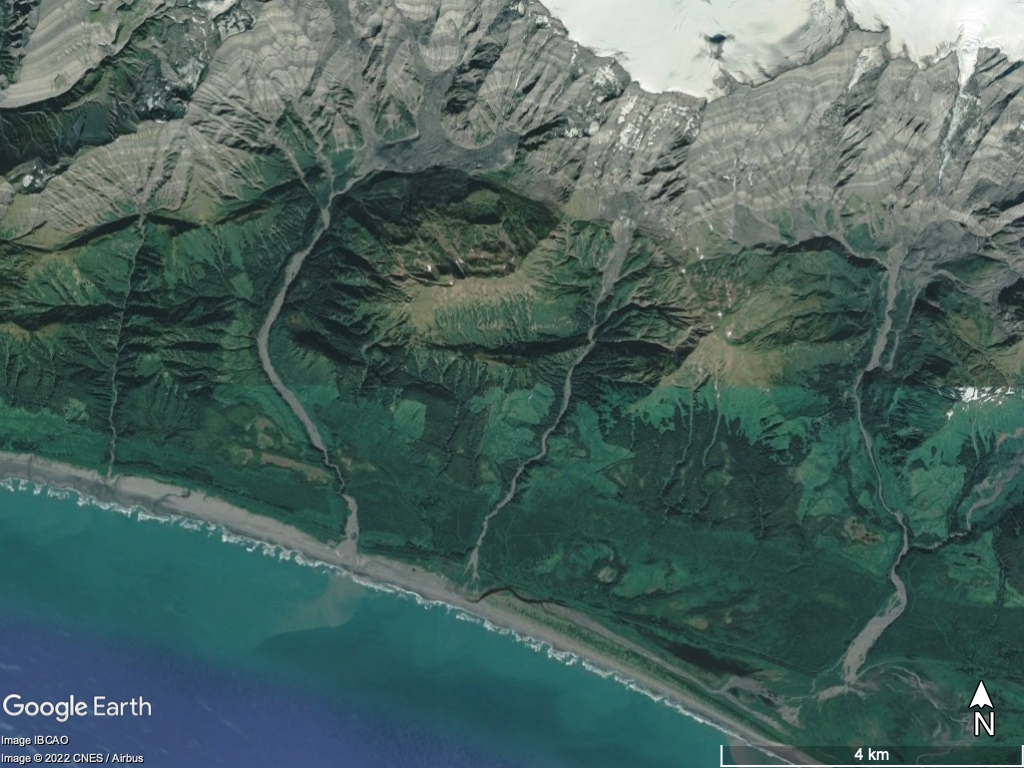
\includegraphics[width=0.48\textwidth]{alaska_googleearth.jpg}} 
	%DIF < 	\caption{Satellite imagery of grid boxes in \textit{(a)} the Southern coast of Victoria, Australia, \textit{(b)} Siberut Island, Indonesia  and \textit{(c)} the Alaskan Gulf. For \textit{(a)} and \textit{(b)} it is expected according to the updated V20 fields that there is no vegetation, just bare ground. For \textit{(c)} it is expected that there is no vegetation and a large fraction of ice.  Evidently, the V20 fields for these grid boxes points are insufficiently accurate, as identified by VESPER. } 
	%DIF < 	\label{fig:cvh}
	%DIF < \end{figure}
	\DIFdelbegin %DIFDELCMD < 

%DIFDELCMD < 	\noindent %%%
\DIFdel{From  this example deploying VESPER on the lake parametrisation fields, }\DIFdelend \DIFaddbegin \subsection{\DIFadd{Evaluation of new lake fields: Monthly water \& salt lakes}}
\DIFadd{From  the examples  above  }\DIFaddend it  is  evident  that  VESPER  enables  the  user  to  quickly  identify  regions  where  the  \DIFdelbegin \DIFdel{new parametrisation works effectively }\DIFdelend \DIFaddbegin \DIFadd{update  to  surface physiographic fields was beneficial }\DIFaddend (e.g. Aral Sea) \DIFdelbegin \DIFdel{as well as spotting regions where it is less performant }\DIFdelend \DIFaddbegin \DIFadd{and where it was not }\DIFaddend (e.g. Lake Natron\DIFdelbegin \DIFdel{, high vegetation updates}\DIFdelend ). In turn, \DIFdelbegin \DIFdel{those areas where the }\DIFdelend \DIFaddbegin \DIFadd{areas where LST }\DIFaddend predictions do not improve as expected can be inspected and erroneous or sub-optimal representations of the surface  \DIFaddbegin \DIFadd{physiographic  }\DIFaddend fields  identified.  This  then  provides  key  information  on  how  \DIFdelbegin \DIFdel{to introduce further }\DIFdelend \DIFaddbegin \DIFadd{and  where  to  introduce  additional }\DIFaddend corrections to better represent these more \DIFdelbegin \DIFdel{difficult }\DIFdelend \DIFaddbegin \DIFadd{challenging }\DIFaddend or complex regions. \DIFdelbegin \DIFdel{We will now further explore some }\DIFdelend \DIFaddbegin \DIFadd{Some }\DIFaddend of these problematic areas \DIFdelbegin \DIFdel{and demonstrate how VESPER can guide the development and introduction of additional surface fields.
	}\DIFdelend \DIFaddbegin \DIFadd{are now explored in more details and additional surface physiographic fields introduced with help of VESPER. }\newline 

\DIFaddend 

\DIFdelbegin \subsection{\DIFdel{V20X: Monthly water \& salt lakes}}
	%DIFAUXCMD
\addtocounter{subsection}{-1}%DIFAUXCMD
%DIFDELCMD < \noindent %%%
\DIFdelend Particular regions where \DIFdelbegin \DIFdel{it was difficult for the model to make predictions - }\DIFdelend \DIFaddbegin \DIFadd{VESPER was struggling to make accurate LST predictions – }\DIFaddend especially with the updated V20 \DIFdelbegin \DIFdel{fields }\DIFdelend \DIFaddbegin \DIFadd{field set }\DIFaddend which only include permanent water \DIFdelbegin \DIFdel{- }\DIFdelend \DIFaddbegin \DIFadd{– }\DIFaddend were either areas with a large degree of temporal variability (e.g. lakes which flood and dry out periodically\DIFdelbegin \DIFdel{, or freeze and melt}\DIFdelend ) or else \DIFdelbegin \DIFdel{lakes which are salt water rather than fresh water }\DIFdelend \DIFaddbegin \DIFadd{areas with saline rather than freshwater }\DIFaddend lakes. Clearly if the size, shape and depth of a lake are changing over the course of the year, these are going to be hugely significant factors in modelling the lake temperature response. Similarly, saline lakes behave very differently to \DIFdelbegin \DIFdel{fresh water }\DIFdelend \DIFaddbegin \DIFadd{freshwater }\DIFaddend lakes since increased salt concentrations affect the density, specific heat capacity, thermal conductivity, and turbidity, as well as evaporation rates, ice formation and ultimately the surface temperature. These two properties of time variability and salinity are often related; it is common for saline lakes to flood and dry out over the course of the season, which naturally also affects the relative saline concentration of the lake itself. \newline 


\DIFdelbegin %DIFDELCMD < \noindent %%%
\DIFdelend Currently, neither \DIFdelbegin \DIFdel{the }\DIFdelend \DIFaddbegin \DIFadd{VESPER\_}\DIFaddend V15 or \DIFaddbegin \DIFadd{VESPER\_}\DIFaddend V20 \DIFdelbegin \DIFdel{models }\DIFdelend have any information regarding the salinity of the lakes or their time variability. Indeed, FLake is specifically a fresh water lake model! \DIFdelbegin \DIFdel{We can introduce this information by also }\DIFdelend \DIFaddbegin \DIFadd{This information can be introduced by }\DIFaddend including a global \DIFdelbegin \DIFdel{salt lake map and monthly inland water lake map as }\DIFdelend \DIFaddbegin \DIFadd{saline lake cover and monthly varying lake cover as additional VESPER’s }\DIFaddend input features, and \DIFdelbegin \DIFdel{use VESPER to investigate the added value of these additional fields .  To create a monthly inland water map we first create 12 monthly fractional land sea masks based on JRC Monthly Water History v1.3 maps for 2010-2020. Since the annual lake maps were created taking into account a lot of additional sources we enforce the extra condition on the monthly maps that the monthly water is equal or greater than permanent water distribution from fractional land sea mask. To create an inland salt water map we used the salt lake list from GLDBv3. First, in order to identify separate lakes on inland water map, we mask small sub-grid lakes and large lake coasts, i. e. grid-cells that have water fraction less than 0.25. Next, we compute number of connected grid-cells in each lake (i.e. connected with sides only). Then we vectorise only lakes that have 100 and more connected grid-cells, as at ERA5 resolution of $\sim$ 31 km the grid-cells are quite large and can include a mixture of freshwater and saline lakes. Finally, saline lake vectors are selected by filtering vectors which have no saline lake point located from GLDBv3. This process resulted in a map at ~31 km resolution based on 147 large salt lake vectors. In the future we plan to revisit the map of salt lakes and extend the list to include additional data. }%DIFDELCMD < \newline 
%DIFDELCMD < 	

%DIFDELCMD < 	
%DIFDELCMD < 	
%DIFDELCMD < 	\noindent %%%
\DIFdel{We create a new model iteration ``}\DIFdelend \DIFaddbegin \DIFadd{then using VESPER to rapidly assess the accuracy of these new surface physiography fields and evaluate if their use in the model increase LST predictability. We define an additional models (see Table \ref{tab:vesper_table} for a summary of all VESPER models used in this work); VESPER\_}\DIFaddend V20X \DIFdelbegin \DIFdel{" which is analogous to the }\DIFdelend \DIFaddbegin \DIFadd{uses the same field set is the same as VESPER\_}\DIFaddend V20 \DIFdelbegin \DIFdel{model, but now also has as input features the monthly water (a quasi-time variable field) and the salt lake cover (a static field). We again train the model on 2016 and make predictions for 2019. The results are presented alongside the }\DIFdelend \DIFaddbegin \DIFadd{but with additional saline lake cover and monthly-varying lake cover. The results of this model in comparison with VESPER\_V15 and VESPER\_}\DIFaddend V20 \DIFdelbegin \DIFdel{results in Table \ref{tab:V1520_results}.

}%DIFDELCMD < \newline 
%DIFDELCMD < 	%%%
\DIFdelend \DIFaddbegin \DIFadd{is summarised in Tables \ref{tab:categorisation}, \ref{tab:categorisation2} . We will now explore the influence of the additional saline maps and monthly lake maps in more detail.

}\DIFaddend 

\subsubsection{Category: Lake \DIFdelbegin \DIFdel{Updates}\DIFdelend \DIFaddbegin \DIFadd{updates}\DIFaddend }\DIFdelbegin %DIFDELCMD < \label{V20XLake}
%DIFDELCMD < 	

%DIFDELCMD < 	\noindent %%%
\DIFdel{We can see that for the }\DIFdelend \DIFaddbegin \label{sec:lake2}
\DIFadd{The }\DIFaddend Lake Updates category \DIFdelbegin \DIFdel{, the prediction accuracy averaged over the year is effectively unchanged from the }\DIFdelend \DIFaddbegin \DIFadd{shows no significant difference in LST predictability globally when using the V20X field set instead of }\DIFaddend V20\DIFdelbegin \DIFdel{model}\DIFdelend \DIFaddbegin \DIFadd{, with $\delta_{\rm V20X} = \delta_{\rm V20} = -0.37$ (comparable training noise)}\DIFaddend . For the \DIFdelbegin \DIFdel{Lake-Ground Updates category, the accuracy has decreased slightly, from $\delta_{\rm V20} = -1.12$ K to   $\delta_{\rm V20X} = -1.09$ K, although the difference is so small as to be within the model noise.
The equivalence of the annually averaged V20X and }\DIFdelend \DIFaddbegin \DIFadd{Lake-ground category, there is a modest increase, with $\delta_{\rm V20X} = -0.84$ compared to   $\delta_{\rm V20} = -0.83$ but this is within the training noise.
}\begin{table*}
	\begin{tabular}{clcccccccc}
		\toprule
		\multirow{2}{*}{Category} & \multirow{2}{*}{Grid-cells/location} & 	\multicolumn{4}{c}{$\sigma_{\rm VM}$, $K$} &&\multicolumn{3}{c}{$\delta_{\rm VM}$, $K$} \\  
		&&\DIFaddFL{V15  }& \DIFaddFL{V15X }& \DIFaddendFL V20 \DIFdelbeginFL \DIFdelFL{models is something that we will return to later in Section \ref{sec:timeseries} when we consider the time-variability of the prediction error. If for now instead of a globally averaged metric, we focus on the problematic points that we discussed previously, then }\DIFdelendFL \DIFaddbeginFL & \DIFaddendFL V20X \DIFdelbeginFL \DIFdelFL{demonstrates a significant improvement over }\DIFdelendFL \DIFaddbeginFL && \DIFaddFL{V15X }&\DIFaddendFL V20 \DIFdelbeginFL \DIFdelFL{for all considered grid points, as illustrated in Table \ref{tab:lake_v20X}. 
	}%DIFDELCMD < \begin{table*}
%DIFDELCMD < 		\centering
%DIFDELCMD < 		\begin{tabular}{lccc}
%DIFDELCMD < 			%%%
\DIFdelFL{Grid Point }\DIFdelendFL & \DIFdelbeginFL \DIFdelFL{$\delta_{\rm V20}$ (K) }\DIFdelendFL \DIFaddbeginFL \DIFaddFL{V20X  }\\
		\hline 
		\multirow{9}{*}{Lake}\DIFaddendFL &\DIFdelbeginFL \DIFdelFL{$\delta_{\rm V20X}$ (K)  }\DIFdelendFL \DIFaddbeginFL \DIFaddFL{Gujarat Province, India}\DIFaddendFL & \DIFdelbeginFL \DIFdelFL{$\delta_{\rm V15X}$ (K) }\DIFdelendFL \DIFaddbeginFL \DIFaddFL{2.54 }&\DIFaddFL{1.12 }&\DIFaddFL{0.42 }&\DIFaddFL{1.04 }&& \DIFaddFL{-1.26 }&\DIFaddFL{4.21}& \DIFaddFL{5.24 }\DIFaddendFL \\
		\DIFdelbeginFL %DIFDELCMD < \hline
%DIFDELCMD < 			%%%
\DIFdelFL{Lake Natron, centre       }\DIFdelendFL &\DIFdelbeginFL \DIFdelFL{5.40 }\DIFdelendFL \DIFaddbeginFL \DIFaddFL{Great Salt Lake Desert, Utah}\DIFaddendFL &\DIFdelbeginFL \DIFdelFL{2.80  }\DIFdelendFL \DIFaddbeginFL \DIFaddFL{0.26 }\DIFaddendFL &\DIFdelbeginFL \DIFdelFL{0.68 }\DIFdelendFL \DIFaddbeginFL \DIFaddFL{0.41 }&\DIFaddFL{0.92 }&\DIFaddFL{0.62 }&& \DIFaddFL{-0.18 }&\DIFaddFL{2.92 }&\DIFaddFL{0.25}\DIFaddendFL \\
		\DIFdelbeginFL \DIFdelFL{Lake Natron, north          }\DIFdelendFL \DIFaddbeginFL &\DIFaddFL{Lake Natron centre, Tanzania}\DIFaddendFL &\DIFdelbeginFL \DIFdelFL{1.66 }\DIFdelendFL \DIFaddbeginFL \DIFaddFL{0.12 }\DIFaddendFL &\DIFdelbeginFL \DIFdelFL{1.54   }\DIFdelendFL \DIFaddbeginFL \DIFaddFL{1.48 }\DIFaddendFL &\DIFdelbeginFL \DIFdelFL{1.10 }\DIFdelendFL \DIFaddbeginFL \DIFaddFL{0.81}& \DIFaddFL{0.53 }&& \DIFaddFL{1.35}& \DIFaddFL{2.45}& \DIFaddFL{2.61 }\DIFaddendFL \\
		\DIFdelbeginFL \DIFdelFL{Lake Blanche                  }\DIFdelendFL &\DIFdelbeginFL \DIFdelFL{1.79  }\DIFdelendFL \DIFaddbeginFL \DIFaddFL{Lake Natron north, Tanzania}\DIFaddendFL &\DIFdelbeginFL \DIFdelFL{-0.64 }\DIFdelendFL \DIFaddbeginFL \DIFaddFL{0.13 }\DIFaddendFL &\DIFdelbeginFL \DIFdelFL{2.76 }\DIFdelendFL \DIFaddbeginFL \DIFaddFL{0.37 }&\DIFaddFL{0.51}& \DIFaddFL{0.18 }&& \DIFaddFL{0.72 }&\DIFaddFL{1.57 }&\DIFaddFL{1.24 }\DIFaddendFL \\
		\DIFdelbeginFL \DIFdelFL{Great Salt LakeDesert  }\DIFdelendFL &\DIFdelbeginFL \DIFdelFL{1.78  }\DIFdelendFL \DIFaddbeginFL \DIFaddFL{Chott Felrhir}\DIFaddendFL &\DIFdelbeginFL \DIFdelFL{-0.28  }\DIFdelendFL \DIFaddbeginFL \DIFaddFL{0.41 }\DIFaddendFL &\DIFdelbeginFL \DIFdelFL{-0.86  }\DIFdelendFL \DIFaddbeginFL \DIFaddFL{0.57}& \DIFaddFL{0.49}& \DIFaddFL{0.58 }&& \DIFaddFL{0.34 }&\DIFaddFL{2.20}& \DIFaddFL{0.73 }\DIFaddendFL \\
		\DIFdelbeginFL \DIFdelFL{Afghanistan                     }\DIFdelendFL \DIFaddbeginFL &\DIFaddFL{Lake Chad}\DIFaddendFL &\DIFdelbeginFL \DIFdelFL{1.66 }\DIFdelendFL \DIFaddbeginFL \DIFaddFL{0.33 }\DIFaddendFL &\DIFdelbeginFL \DIFdelFL{-0.38  }\DIFdelendFL \DIFaddbeginFL \DIFaddFL{1.21 }\DIFaddendFL &\DIFdelbeginFL \DIFdelFL{-0.16 }\DIFdelendFL \DIFaddbeginFL \DIFaddFL{0.98 }&\DIFaddFL{0.96 }&& \DIFaddFL{0.29 }&\DIFaddFL{1.74 }&\DIFaddFL{0.03}\DIFaddendFL \\
		\DIFdelbeginFL \DIFdelFL{Northern India                 }\DIFdelendFL &\DIFdelbeginFL \DIFdelFL{1.60 }\DIFdelendFL \DIFaddbeginFL \DIFaddFL{Al Fashaga}\DIFaddendFL &\DIFdelbeginFL \DIFdelFL{0.59  }\DIFdelendFL \DIFaddbeginFL \DIFaddFL{0.14 }\DIFaddendFL &\DIFdelbeginFL \DIFdelFL{-5.87 }\DIFdelendFL \DIFaddbeginFL \DIFaddFL{0.08 }&\DIFaddFL{0.29 }&\DIFaddFL{0.42 }&& \DIFaddFL{-0.24}& \DIFaddFL{0.94 }&\DIFaddFL{1.06 }\DIFaddendFL \\
		\DIFdelbeginFL \DIFdelFL{Toshka Lakes                  }\DIFdelendFL &\DIFdelbeginFL \DIFdelFL{1.56 }\DIFdelendFL \DIFaddbeginFL \DIFaddFL{Tersakan Lake}\DIFaddendFL &\DIFdelbeginFL \DIFdelFL{-0.59 }\DIFdelendFL \DIFaddbeginFL \DIFaddFL{0.25 }\DIFaddendFL &\DIFdelbeginFL \DIFdelFL{-0.14 }\DIFdelendFL \DIFaddbeginFL \DIFaddFL{0.20}& \DIFaddFL{0.34 }&\DIFaddFL{0.38 }&& \DIFaddFL{-0.00 }&\DIFaddFL{0.85 }&\DIFaddFL{0.99 }\DIFaddendFL \\
		\DIFaddbeginFL &\DIFaddFL{Lake Urmia}&\DIFaddFL{0.12}& \DIFaddFL{0.54 }&\DIFaddFL{0.73 }&\DIFaddFL{0.32 }&& \DIFaddFL{0.54 }&\DIFaddFL{0.82 }&\DIFaddFL{0.22 }\\
		\DIFaddendFL \hline 
		\DIFaddbeginFL \multirow{2}{*}{Glacier}&\DIFaddFL{Calluqueo Glacier, Patagonia}&\DIFaddFL{0.38 }&\DIFaddFL{0.62}& \DIFaddFL{1.60 }&\DIFaddFL{0.73 }&& \DIFaddFL{0.08}& \DIFaddFL{2.49 }&\DIFaddFL{0.32}\\
		&\DIFaddFL{Juncal Glacier, Chilean Andes }&\DIFaddFL{0.68}& \DIFaddFL{0.29}& \DIFaddFL{1.06}& \DIFaddFL{0.36 }&& \DIFaddFL{0.11 }&\DIFaddFL{1.26 }&\DIFaddFL{1.20 }\\
		\bottomrule
	\DIFaddendFL \end{tabular}
	\caption{\DIFdelbeginFL \DIFdelFL{$\delta_{\rm M}$ values }\DIFdelendFL \DIFaddbeginFL \DIFaddFL{As Table \ref{tab:categorisation} }\DIFaddendFL for \DIFdelbeginFL \DIFdelFL{selected }\DIFdelendFL \DIFaddbeginFL \DIFaddFL{specific }\DIFaddendFL grid points \DIFdelbeginFL \DIFdelFL{within }\DIFdelendFL \DIFaddbeginFL \DIFaddFL{discussed in }\DIFaddendFL the \DIFdelbeginFL \DIFdelFL{Lake Updates category for each of }\DIFdelendFL \DIFaddbeginFL \DIFaddFL{text where }\DIFaddendFL the \DIFdelbeginFL \DIFdelFL{trained }\DIFdelendFL \DIFaddbeginFL \DIFaddFL{VESPER\_}\DIFaddendFL V20 \DIFdelbeginFL \DIFdelFL{/V20X/V15X models}\DIFdelendFL \DIFaddbeginFL \DIFaddFL{predictions are worse than VESPER\_V15 (i}\DIFaddendFL .\DIFdelbeginFL \DIFdelFL{V20X consistently outperforms V20 at these locations, but for some points, }\DIFdelendFL e. \DIFdelbeginFL \DIFdelFL{g}\DIFdelendFL \DIFaddbeginFL \DIFaddFL{$\delta_{\rm V20}$ is positive)}\DIFaddendFL .\DIFdelbeginFL \DIFdelFL{Lake Natron, underperforms the more basic V15 model. Conversely, V15X underperforms V20/V20X globally, but can outperform V15 at some selected points, where the updated V20 fields are less accurate.}\DIFdelendFL }
	\DIFdelbeginFL %DIFDELCMD < \label{tab:lake_v20X}
%DIFDELCMD < 	%%%
\DIFdelendFL \DIFaddbeginFL \label{tab:categorisation2}
\DIFaddendFL \end{table*}
For \DIFdelbegin \DIFdel{Lake Blanche, V20X reduces the prediction error by 2.43K compared to }\DIFdelend \DIFaddbegin \DIFadd{some of the problematic lake grid-cells highlighted in Table \ref{tab:categorisation2}, the addition of saline maps and monthly lake maps does improve the LST predictability relative to VESPER\_}\DIFaddend V20\DIFdelbegin \DIFdel{. This is in-spite of the fact that our salt lake maps do not identify Lake Blanche as a salt lake, and so all the improvement in the prediction is from the additional information from the monthly lake maps. The salt lake maps are similarly inaccurate for the grid point in Northern India, failing to recognise the underlying salt marsh. However, again the information contained in the monthly lake maps allows the reduction in the error by $2.19$K. There are also regions where the saline maps are correct to not specify any salinity, such as in Afghanistan and the Toshka lakes; again the monthly maps provided sufficient information to allow for a marked improvement by $2.04$ K and $2.15$ K respectively. This is particularly notable since the size of the monthly lake corrections is small for these points: the mean monthly correction for Afghanistan is 0.046 and for the Toshka Lakes is 0.001. However, under the updated V20 both of these areas have had all water removed and so adding in just a small amount of time variable water allows for much more accurate predictions. This example illustrates how VESPER both can identify inaccurate fields and quantify the value of updated fields, as well as emphasizing the importance of time variable lake fields more generally. For points where the saline maps do specify that the underlying lakes are salt lakes - Lake Natron and }\DIFdelend \DIFaddbegin \DIFadd{. For the Great }\DIFaddend Salt Lake Desert\DIFdelbegin \DIFdel{- it is not possible to disentangle whether the gain is due to the saline maps or the monthly maps. The centre of Lake Natron exhibits a particularly notable improvement by $2.6$K, whilst for the grid point on the northern edge the gain is more modest at $0.12$K. This is likely due to the fact that the updated monthly maps provided much stronger corrections at the centre of the lake (mean correction 0.13) than at the northern edge (mean correction 0.02). For }\DIFdelend \DIFaddbegin \DIFadd{, Chott Fehlrir, Lake Chad and Lake Urmia, VESPER\_V20X is a notable improvement over VESPER\_V20, with $\delta_{\rm V20X}$ = $0.248,0.726,0.029,0.22$ respectively. The difference in  $\delta_{\rm V20X}$ and $\delta_{\rm V20}$ for these points is greater than }\DIFaddend the \DIFaddbegin \DIFadd{training noise. If we take as a case example the }\DIFaddend grid point \DIFdelbegin \DIFdel{at }\DIFdelend \DIFaddbegin \DIFadd{in }\DIFaddend the Great Salt Lake Desert, the improvement \DIFdelbegin \DIFdel{is $2.06$ K again with }\DIFdelend \DIFaddbegin \DIFadd{in using  VESPER\_V20X over VESPER\_V20 is 2.667K $\pm 1.10$ K. At this point there is }\DIFaddend a strong correction from the monthly lake maps (mean value 0.16) and the salt maps (mean value 0.56). This improvement is to be expected given the known strong salinity and time variability in the region, and so it is a nice confirmation to have these updated fields verified by VESPER. It is also notable that the variation in the monthly lake maps at this point is very large, with a standard deviation in the lake fraction over 12 months of 0.18. At the start of the year the corrections from the monthly maps are very large, then as the year progresses the magnitude of the corrections generally decreases as the lake dries out. Such a large variation is again difficult to ever capture with a static field. \newline 

\DIFdelbegin %DIFDELCMD < \noindent %%%
\DIFdel{Other regions of note that we have mentioned previously are the Northwest Territories and the Nunavut province in Northern Canada where the }\DIFdelend \DIFaddbegin \DIFadd{It is however notable that a) for all of the problematic lake points that we have discussed $\delta_{\rm V20X}$ is positive and b) there are multiple points (e.g. Gujarat province) where VESPER\_20X exhibits no improvement over VESPER\_}\DIFaddend V20 \DIFdelbegin \DIFdel{model underperformed relative to V15, with $\delta_{\rm V20} = +0.02$ K. The introduction of the monthly lake maps modestly improves the predictions in this area, with $\delta_{\rm V20X} = -0.03$K.  In these high latitude regions one might expect some time variability due to freezing and thawing of the lake surfaces, and the addition of the monthly lake maps to the model then provides some of this time variable information, allowing for improved predictions.  Whilst this is an improvement, the effect is modest; it is generally difficult to get quality observations at high latitudes, especially during the cold season, due to increased cloud cover. Therefore whilst VESPER can say that the addition of the monthly lake maps does improves the predictions in these regions, for improved performance cloud independent data should be used.  Additionally, the corrections from the monthly lake maps are small in these regions, with amean correction of 0.02 and a generally small variance; in actuality time variable fields with greater variance over the year may be more accurate. Due to the freezing and thawing, improving ice on/off date prediction by the lake parametrisation should help better describe the seasonality and variance. }%DIFDELCMD < \newline 
%DIFDELCMD < 	

%DIFDELCMD < 	\noindent %%%
\DIFdel{It is worth emphasising that whilst the V20 and V20X models are improvements over V15 globally, and V20X is generally an improvement over V20 for these problematic points, there are regions where neither V20 or V20X outperform V15 ($\delta_{\rm M}$ is always positive) , such as Lake Natron and Northern India}\DIFdelend \DIFaddbegin \DIFadd{within training noise}\DIFaddend . Given all the extra information provided to the more advanced \DIFdelbegin \DIFdel{models }\DIFdelend \DIFaddbegin \DIFadd{VESPER\_20X model }\DIFaddend this is unusual\DIFdelbegin \DIFdel{, unless }\DIFdelend \DIFaddbegin \DIFadd{; it suggests that either i) some of }\DIFaddend the additional information is erroneous in these regions\DIFdelbegin \DIFdel{or else }\DIFdelend \DIFaddbegin \DIFadd{, or else ii) }\DIFaddend the temperature response is \DIFdelbegin \DIFdel{completely }\DIFdelend atypical to the rest of the globe\DIFdelbegin \DIFdel{and }\DIFdelend \DIFaddbegin \DIFadd{. For point ii), this means that }\DIFaddend the additional information is not predictive in these regions. \DIFdelbegin \DIFdel{To explore this hypotheses we }\DIFdelend \DIFaddbegin \DIFadd{Including this additional information in our neural network increases the complexity of the model which may in turn increase its training noise. This is likely the reason behind point b) - the updated fields are not sufficiently informative but do increase the training noise and so we see no improvement from using VESPER\_V20X. For example, for Gujarat province $\sigma_{\rm V20} = 0.416$, but $\sigma_{\rm V20X} = 1.04$. In order to explore the hypothesis of point i) we }\DIFaddend train one further model, \DIFaddbegin \DIFadd{VESPER\_}\DIFaddend V15X \DIFdelbegin \DIFdel{. This }\DIFdelend \DIFaddbegin \DIFadd{(again, see Table \ref{tab:vesper_table} for a summary of all VESPER models used in this work). This VESPER iteration }\DIFaddend is analogous to \DIFaddbegin \DIFadd{VESPER\_}\DIFaddend V20X, being simply the \DIFaddbegin \DIFadd{VESPER\_}\DIFaddend V15 model with the additional monthly maps and salt lake fields included. Importantly it does not have the updated \DIFaddbegin \DIFadd{physiographic }\DIFaddend correction fields from V20. Globally, this model performs worse that the V20 models, as we might expect - for example in the Lake Updates category \DIFdelbegin \DIFdel{$\delta_{\rm V15X} = -0.25$K compared to $\delta_{\rm 20X} = -0.45$ }\DIFdelend \DIFaddbegin \DIFadd{$\delta_{\rm V15X}$ = −0.20 ($\sigma_{\rm V15X} = 0.02$) compared to $\delta_{\rm V20}$= −0.37 }\DIFaddend K. However, \DIFaddbegin \DIFadd{VESPER\_}\DIFaddend V15X does perform well at \DIFdelbegin \DIFdel{these problematic }\DIFdelend \DIFaddbegin \DIFadd{a number of the these problematic lake }\DIFaddend points (see Table \DIFdelbegin \DIFdel{\ref{tab:lake_v20X}}\DIFdelend \DIFaddbegin \DIFadd{\ref{tab:categorisation2}}\DIFaddend ). For \DIFdelbegin \DIFdel{both the Lake Natron grid pointsV15 outperforms }\DIFdelend \DIFaddbegin \DIFadd{7 out of the 9 selected lake points, VESPER\_V15X outperforms VESPER\_}\DIFaddend V20X\DIFdelbegin \DIFdel{, suggesting that at this location }\DIFdelend \DIFaddbegin \DIFadd{. For example in Gujarat province the improvement in using V15X over V20X is $6.5K \pm 1.53$. This suggests that our hypothesis for point i) is correct and that for some grid points }\DIFaddend the V20 fields are \DIFdelbegin \DIFdel{generally }\DIFdelend less accurate than the V15 fields. \DIFaddbegin \DIFadd{For a subset of points VESPER\_}\DIFaddend V15X \DIFdelbegin \DIFdel{however underperforms relative to }\DIFdelend \DIFaddbegin \DIFadd{also outperforms VESPER\_}\DIFaddend V15 \DIFdelbegin \DIFdel{which also indicates that the monthly maps and the salt lakes are either inaccurate at this location, or that the temperature response of Lake Natron is highly atypical.For Northern India, the performance of the V15 model is particularly striking; whilst the V20 and V20X models struggled to make more accurate predictions than V15, V15X decreases the average prediction error by nearly 6K.This again indicates that for this point the V20 fields are less accurate than V15. Similarly for the Great Salt Lake Desert, $\delta_{\rm V20} = 1.78$ K, $\delta_{\rm V20X} = -0.28$ K but $\delta_{\rm V15X} = -0.86$ K, which suggests that whilst the monthly lake maps and the salt lake fractions are accurate and informative in this area, the static V20 fields are not}\DIFdelend \DIFaddbegin \DIFadd{(e.g. for Gujarat province $\delta_{\rm V15X} = -1.26$) but the difference is typically within or close to the training noise (e.g. for Gujarat $\sigma_{\rm V15X} = 1.12$) and so it is hard to draw any strong conclusions}\DIFaddend .  These examples illustrates again how VESPER can identify particular regions where the fields are inaccurate, as well as emphasising the need more generally for accurate descriptions of seasonally varying inland water and saline lake maps in Earth system modelling.

\DIFdelbegin %DIFDELCMD < \newline 
%DIFDELCMD < 	%%%
\DIFdelend 

\subsubsection{Category: Vegetation Updates}
Whilst the Vegetation Updates category explicitly deals with areas where the lake fraction does not change when going from V15 to V20, many of the grid points in this category do contain some kind of waterbody, often lying close to the coast or else containing lakes or large rivers. Information on the salinity and temporal variability of these water bodies \DIFdelbegin \DIFdel{can }\DIFdelend \DIFaddbegin \DIFadd{could }\DIFaddend then influence the prediction accuracy. By providing the additional information in \DIFdelbegin \DIFdel{V20X, the mean $\delta_{M}$ is reduced from $\delta_{\rm V20} = +0.049$K to $\delta_{\rm V20X} =0.005 $K. This performance is gained despite the known errors for some of the grid boxes in the }\textit{\DIFdel{cvh}} %DIFAUXCMD
\DIFdel{vegetation updates (e.g. Figure \ref{fig:cvh}), again demonstrating the importance of salinity and seasonally varying water. The V15X model is less performant than V20X, with $\delta_{\rm V15X} = 0.11$K since there }\textit{\DIFdel{are}} %DIFAUXCMD
\DIFdel{some grid boxes in this category where the updated V20 fields are accurate and valuable if augmented by monthly variability. However if we consider just the worst performing grid points where $\delta_{\rm V20} > 1$ K then the mean values are $\delta_{\rm V20} = 2.0$ K, $\delta_{\rm V20X} = 0.49$ K and $\delta_{\rm V15X} = 0.21$K.

This again demonstrates how the }\textit{\DIFdel{cvh}} %DIFAUXCMD
\DIFdel{fields have been erroneously updated for a small selection of grid points in V20. 
	}\DIFdelend \DIFaddbegin \DIFadd{VESPER\_20X, the error relative to  VESPER\_V15 is reduced modestly to $-3 \times 10^{-4}$ although as we saw before with the vegetation category the noise is large $\sigma_{\rm V20X} = 0.21$ and so it is difficult to draw any further definitive conclusions. Similar arguments apply to VESPER\_15X.

}\DIFaddend 


\subsubsection{Category: Glacier Updates}
We would expect the additional information provided by \DIFaddbegin \DIFadd{the }\DIFaddend V20X \DIFaddbegin \DIFadd{fields }\DIFaddend to be particularly effective for glacial grid points. Glacier ice is naturally found next to waterbodies which freeze and thaw over the year, and the salinity of water will also influence this freezing. Therefore accurate additional information from the monthly lake maps and the saline maps should prove useful in these more time variable regions. \DIFdelbegin \DIFdel{This is indeed what we observe with the mean delta going from $\delta_{\rm V20} = -0.13$K to $\delta_{\rm V20X}= -0.24$K.  Considering the two problematic points that we discussed previously, in the Alaskan Gulf the prediction accuracy relative to V15 has improved from $\delta_{\rm V20} = +2.16$ K to $\delta_{\rm V20X}= +1.00$ K, whilst for the Juncal Glacier }\DIFdelend \DIFaddbegin \DIFadd{We do observe a small improvement globally, with $\delta_{\rm V20X} = -0.28$ compared to $\delta_{\rm V20} = -0.22$, however this difference is comparable to }\DIFaddend the \DIFdelbegin \DIFdel{prediction accuracy has also improved, with $\delta_{\rm V20X}$ decreasing to $+1.88$ K. Despite this improvement, again for both of these points the prediction accuracy still lags behind V15. This is on account of the }\DIFdelend \DIFaddbegin \DIFadd{training noise $\sigma_{\rm V20X} = 0.06$. This training noise could be slightly deceptive;  3 out of our 4 VESPER\_V20X iterations outperform every VESPER\_}\DIFaddend V20 \DIFdelbegin \DIFdel{fields being insufficiently accurate in these areas, as has been discussed. Neither of these grid points correspond to saline lakes or have a significant time variability in }\DIFdelend \DIFaddbegin \DIFadd{iteration in the Glacier Updates category. The 4th VESPER\_V20X iteration is somewhat anomalous - the increased network complexity could mean that the model did not converge well for that particular iteration, for }\DIFaddend the \DIFdelbegin \DIFdel{monthly lake fractions and so are also not improved by a }\DIFdelend \DIFaddbegin \DIFadd{glacier grid points. Since the updated V20 glacier fields are generally accurate globally, we saw no particular  improvement in using VESPER\_}\DIFaddend V15X \DIFdelbegin \DIFdel{model. }\DIFdelend \DIFaddbegin \DIFadd{to within the training noise. This suggests that the additional monthly lake maps are only useful if the underlying representation of static water is sufficiently accurate. Considering the particular glacier grid points we discussed previously in Section \ref{sec:glacier}, the additional monthly lake maps were particularly useful for the Calluqueo glacier, with $\delta_{\rm V20X} = 0.32$ compared to $\delta_{\rm V20} = 2.49$ ($\sigma_{\rm V20}=1.59$, $\sigma_{\rm V20X}=0.73$). However we saw no improvement to within the training noise for the Juncal glacier 

}\DIFaddend 

%DIF < For the Alaskan Gulf, the improvement through the introduction of the monthly lake maps (salt fields here are zero) suggests that again this is a grid point where the variability in the surface water strongly influences the skin temperatures. Indeed, this grid point lies at a high latitude ($\sim 60^{\circ}$ N) where the surface will freeze and thaw over the course of a year, naturally influencing the surface water fraction. For the Kerguelen Islands, the V20X prediction is still worse than V15. If we deploy V15X then the error is strongly reduced to $-0.91$. This again is good evidence that the updated V20 surface fields, such as the glacial fraction are less accurate for this particular grid point.
	\DIFdelbegin %DIFDELCMD < 

%DIFDELCMD < 	
%DIFDELCMD < 	
%DIFDELCMD < 	%%%
\DIFdelend \subsubsection{Timeseries}
\DIFdelbegin %DIFDELCMD < \label{sec:timeseries}
%DIFDELCMD < 	

%DIFDELCMD < 	
%DIFDELCMD < 	\noindent %%%
\DIFdelend Thus far we have been focusing mainly on the \DIFdelbegin \DIFdel{$\delta_{\rm M}$ }\DIFdelend \DIFaddbegin \DIFadd{$\delta_{\rm VM}$ }\DIFaddend metric averaged over the entire year of the test set. It is also of interest to explore how the prediction error for each of the 3 models varies with time. This is demonstrated in Fig \ref{fig:timeseries} for each of the 4 updated categories that we have discussed. \newline 

\noindent For the Lake Updates and Lake-Ground Updates categories we can see that all the model predictions track the same general profile, with the error peaking in the northern hemisphere summer months. This is a result of FLake modelling being least accurate during the summer as the lake is not fully mixed and so the mixed layer depth for lakes is too shallow, resulting in skin temperatures with larger errors. Conversely, in the autumn and spring the lake is fully mixed and predictions have the smallest errors compared with observations. A clear hierarchy of models is evident; the \DIFaddbegin \DIFadd{VESPER\_V15 and VESPER\_}\DIFaddend V20 \DIFdelbegin \DIFdel{/V20X }\DIFdelend models consistently outperform \DIFdelbegin \DIFdel{the }\DIFdelend \DIFaddbegin \DIFadd{VESPER\_}\DIFaddend V15 \DIFdelbegin \DIFdel{model }\DIFdelend across the year. This again is \DIFdelbegin \DIFdel{solid }\DIFdelend \DIFaddbegin \DIFadd{strong }\DIFaddend evidence, highlighted by VESPER, of the value of the updated fields both static and seasonally varying. We \DIFdelbegin \DIFdel{mentioned }\DIFdelend \DIFaddbegin \DIFadd{discussed }\DIFaddend previously how the annually and globally averaged \DIFdelbegin \DIFdel{$\delta_{\rm M}$ }\DIFdelend \DIFaddbegin \DIFadd{$\delta_{\rm VM}$ }\DIFaddend values for the Lake Updates category were highly comparable for \DIFaddbegin \DIFadd{VESPER\_}\DIFaddend V20 and \DIFaddbegin \DIFadd{VESPER\_}\DIFaddend V20X\DIFdelbegin \DIFdel{, despite V20X significantly improving the worst behaving points}\DIFdelend . We can see from the top panel in Figure \ref{fig:timeseries} that \DIFdelbegin \DIFdel{the }\DIFdelend \DIFaddbegin \DIFadd{this equivalence is not consistent over the year. Instead, during the winter months of the northern hemisphere  VESPER\_V20 and VESPER\_}\DIFaddend V20X \DIFdelbegin \DIFdel{model is a systematic improvement on }\DIFdelend \DIFaddbegin \DIFadd{are fairly equivalent;  VESPER\_}\DIFaddend V20 \DIFdelbegin \DIFdel{from around April onwards, but at earlier times in the year V20 outperforms }\DIFdelend \DIFaddbegin \DIFadd{tends to outperform VESPER\_V20X, but the difference is within the model training noise. However in the central months of the year VESPER\_}\DIFaddend V20X \DIFaddbegin \DIFadd{starts to be slightly more accurate}\DIFaddend . This is likely for two reasons. Firstly, the monthly lake maps are in fact a climatology and therefore insufficiently precise to detect the exact ice on/off dates during the winter months, where we have a large number of grid points at high latitudes which will be subject to freezing, nullifying any time variability. \DIFdelbegin \DIFdel{Secondly, }\DIFdelend \DIFaddbegin \DIFadd{The second reason is }\DIFaddend due to the accuracy of the lake mean depth which strongly drives the ice on-dates due to its influence on the heat capacity of the lake. During the warmer months lakes thaw, the monthly maps are more accurate, as the thawing of lake ice is mainly connected to the atmospheric conditions, not the lake depth, and so the information contained in them can be used to make more accurate predictions. \DIFaddbegin \newline 

\DIFaddend The Lake-Ground Updates timeseries broadly follows the same general profile as Lake Updates, but the errors are larger - those grid points where the lakes have been replaced with bare ground were particularly poorly described in V15. Additionally, for Lake Updates we see two sharp decreases in the prediction error during \DIFdelbegin \DIFdel{$\sim$ }\DIFdelend \DIFaddbegin \DIFadd{∼ }\DIFaddend April and September, which are not as strongly reflected in Lake-Ground. This is due to the geographic location of the grid points in each of the two categories; for the Lake Updates category the grid points are located primarily in the boreal zones and so are subject to freezing and thawing over the course of the year leading to a strong seasonality due to the lake mixing that we have discussed. The sharp drop in April corresponds to a time where the lakes are unfrozen and fully mixed. However the lakes in the Lake-Ground sub-category are less concentrated and much more evenly distributed over the globe and so do not exhibit such a strong seasonality. \DIFdelbegin %DIFDELCMD < \newline 
%DIFDELCMD < 	

%DIFDELCMD < 	
%DIFDELCMD < 	
%DIFDELCMD < 	\noindent %%%
\DIFdel{Examining the timeseries for Vegetation Updates, whilst there is a large degree of variability, we again see the trend previously discussed whereby the V20 fields make the predictions systematically worse across the entirety of the test year. The introduction of the monthly lake maps in V20X compensates for the erroneous V20 vegetation fields - the V20X predictions are generally worse than V15 at the start and end of the year, but better in the middle. This is due to the fact that the majority of }\DIFdelend \DIFaddbegin \DIFadd{Consistent with our previous discussion, }\DIFaddend the \DIFdelbegin \DIFdel{points in the Vegetation Updates category are in climate zones which have pronounced rainy and dry seasons e.g. Indonesia, the Amazon. At the start }\DIFdelend \DIFaddbegin \DIFadd{training noise makes it difficult to separate the predictions }\DIFaddend of the \DIFaddbegin \DIFadd{VESPER model for the vegetation category across the }\DIFaddend year\DIFdelbegin \DIFdel{during }\DIFdelend \DIFaddbegin \DIFadd{. All generations of VESPER\_VM follow the same general trend, with errors maximal at the start and end of }\DIFaddend the \DIFdelbegin \DIFdel{wet season there is lots of precipitation and the static V15 fields are generally more accurate. As the rains abate and the dry season starts the V15 lake fields are underestimates which are then improved through the introduction of additional water via the monthly lake maps. }\DIFdelend \DIFaddbegin \DIFadd{year, and minimal during the spring and autumn months. }\DIFaddend \newline 

\DIFdelbegin %DIFDELCMD < \noindent %%%
\DIFdel{For Glacier updates we can }\DIFdelend \DIFaddbegin \DIFadd{For the Glacier updates category, in order to deal with the separate warming and cooling seasonal cycles over the year, we }\DIFaddend separate grid points into the northern and southern hemispheres. \DIFdelbegin \DIFdel{We again consider just those points where the number of MODIS observations at a given instant in time, per ERA data point is greater than 50. }\DIFdelend For the northern hemisphere the \DIFdelbegin \DIFdel{familiar hierarchy of models is recovered, with the V20X model generally outperforming V20, which in turn generally outperforms V15. The }\DIFdelend errors peak for all models in the summer, again due to the lakes not being fully mixed. There is also an uptick in the prediction error for all models during the winter when the freezing is greatest - this indicates how ice cover can strongly influence the \DIFdelbegin \DIFdel{land surface temperature response. }\DIFdelend \DIFaddbegin \DIFadd{LST response. The familiar hierarchy of models is recovered; VESPER\_V15 is generally outperformed by the more updated models. In turn VESPER\_V20X is a general improvement over VESPER\_V20 throughout the year, especially during the winter months where the training noise is minimal. Since this is the time when freezing is greatest, this suggests that the additional monthly maps and salt lake maps are particularly useful during this time. }\DIFaddend For the southern hemisphere the story is different. The errors are smallest during the middle of the year when we expect the freezing to be greatest. During the spring and autumn the errors are largest - this is correlated with a decrease in the number of observations suggesting that this is due to poorer data quality due to cloud cover. In the summer when the weather is clearer the errors start to decrease again. Given this variation in the data quality due to cloud cover it is difficult to draw any strong conclusions, and again for stronger performance cloud independent data should be used. What is obvious for the southern hemisphere glacier grid points is that the \DIFaddbegin \DIFadd{VESPER\_}\DIFaddend V20 and \DIFaddbegin \DIFadd{VESPER\_}\DIFaddend V20X models struggle to improve on \DIFaddbegin \DIFadd{VESPER\_}\DIFaddend V15, unlike in the northern hemisphere. This suggests that the updated V20 fields are still insufficiently accurate for southern latitudes. \newline 

\DIFdelbegin %DIFDELCMD < \begin{figure}
%DIFDELCMD < 		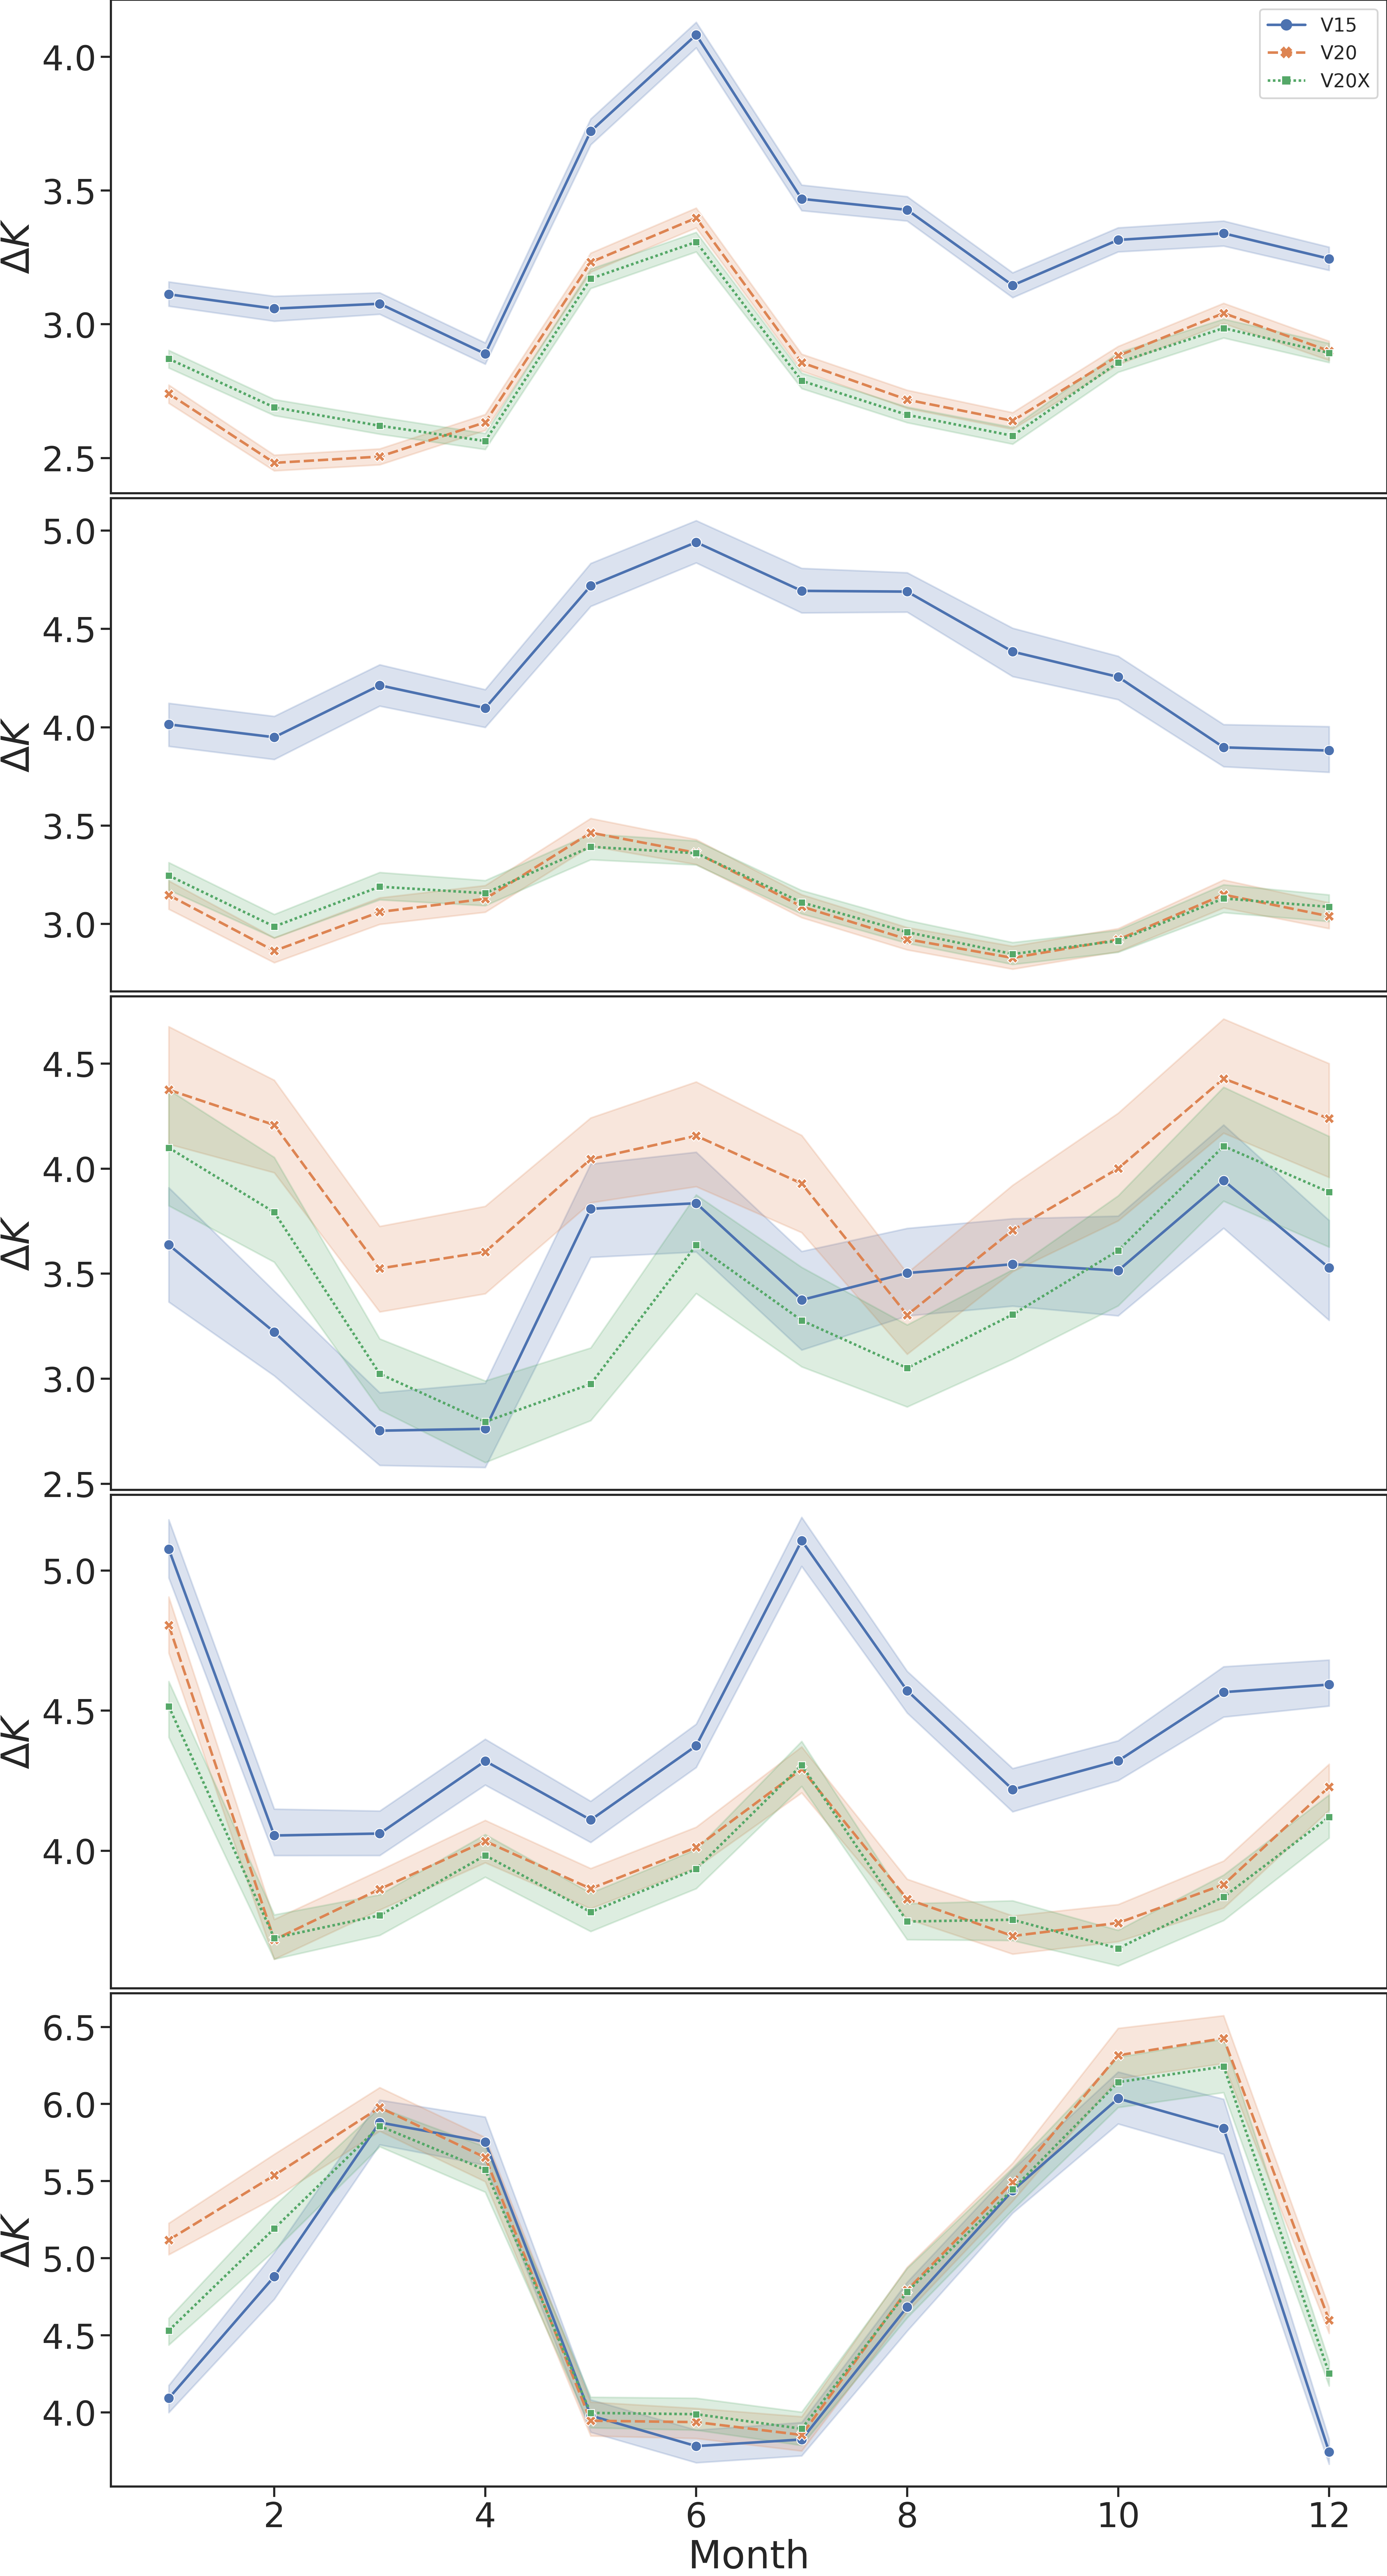
\includegraphics[width=\columnwidth]{mega_stack_ns.png}
%DIFDELCMD < 		%%%
%DIFDELCMD < \caption{%
{%DIFAUXCMD
\DIFdelFL{Mean prediction error in the surface temperature $\bar{\Delta} K$, averaged over all grid points, for each of the 3 models over the course of the test year for (}\textit{\DIFdelFL{top panel}}%DIFAUXCMD
\DIFdelFL{) Lake Updates, (}\textit{\DIFdelFL{second panel}}%DIFAUXCMD
\DIFdelFL{) Lake-Ground Updates, (}\textit{\DIFdelFL{third panel}}%DIFAUXCMD
\DIFdelFL{) Vegetation Updates, (}\textit{\DIFdelFL{fourth panel}}%DIFAUXCMD
\DIFdelFL{) Glacier Updates, northern hemisphere and (}\textit{\DIFdelFL{bottom panel}}%DIFAUXCMD
\DIFdelFL{) Glacier Updates, southern hemisphere. For the Glacier Updates category we again exclude grid points where the number of MODIS observations per ERA data point is less than 50.  For the Lake categories, all models follow the same general profile, with the V20X model generally outperforming the V20 model over the year, which in turn outperforms the V15 model. The value of the additional V20 correction fields and the V20X monthly lake maps and salt lake maps, is evident.}}
		%DIFAUXCMD
%DIFDELCMD < \label{fig:timeseries}
%DIFDELCMD < 	\end{figure}
%DIFDELCMD < 	%%%
\DIFdelend 


\DIFdelbegin %DIFDELCMD < \noindent %%%
\DIFdelend We have also discussed previously particular grid points \DIFdelbegin \DIFdel{where there is expected to be }\DIFdelend \DIFaddbegin \DIFadd{that will likely show }\DIFaddend a large degree of temporal variability\DIFaddbegin \DIFadd{, }\DIFaddend or the lakes are saline\DIFaddbegin \DIFadd{, }\DIFaddend and as a consequence the static \DIFaddbegin \DIFadd{physiographic }\DIFaddend V15/V20 fields struggle to make accurate predictions (e.g. Table \DIFdelbegin \DIFdel{\ref{tab:lake_v20X}}\DIFdelend \DIFaddbegin \DIFadd{\ref{tab:categorisation2}}\DIFaddend ). In Figure \ref{fig:timeseries_stacked} we present timeseries for two of these points: \DIFdelbegin \DIFdel{Lake Natron in Tanzania and  Gujarat Province, India}\DIFdelend \DIFaddbegin \DIFadd{the Great Salt Lake Desert, Utah and  Chott Felrhir, Algeria}\DIFaddend . Both these points were discussed in Sections \DIFdelbegin \DIFdel{\ref{V20Lake} and \ref{V20XLake}}\DIFdelend \DIFaddbegin \DIFadd{\ref{sec:lake1}, \ref{sec:lake2}}\DIFaddend . We can see that for these two selected points the hierarchy of models no longer holds. Whilst there is a large degree of variability, and there is no clear separation between models \DIFdelbegin \DIFdel{that we get when averaging over all grid points as in Fig \ref{fig:timeseries}}\DIFdelend \DIFaddbegin \DIFadd{for some parts of the year}\DIFaddend , generally it can be seen that \DIFaddbegin \DIFadd{VESPER\_V20 performs worse than VESPER\_V15. For the Great Salt Lake }\DIFaddend the \DIFaddbegin \DIFadd{inaccuracy when using the }\DIFaddend V20 \DIFdelbegin \DIFdel{model performs the worst, indicating that the updated fields are not accurate in these regions. For Lake Natron the }\DIFdelend \DIFaddbegin \DIFadd{physiographic fields is most pronounced during the summer months. April, May and June are some of the wettest months in this region. But the updated }\DIFaddend V20 \DIFdelbegin \DIFdel{/V20X models are significantly worse throughout almost the entire year. The updated models - which }\DIFdelend \DIFaddbegin \DIFadd{fields }\DIFaddend specify a much \DIFdelbegin \DIFdel{larger }\DIFdelend \DIFaddbegin \DIFadd{smaller }\DIFaddend lake fraction than in V15 \DIFdelbegin \DIFdel{- perform well at the beginning and start of the year which tend to be the wettest months at Lake Natron. However,  during the summer as the lake dries out the errors grow significantly}\DIFdelend \DIFaddbegin \DIFadd{($\sim 0.5$ compared to $0.0$). Consequently during this time the V20 fields are maximally inaccurate and the prediction error of the VESPER\_V20 model grows accordingly}\DIFaddend .This indicates again that the updated V20 fields are in fact over-corrections for this area. \DIFdelbegin \DIFdel{Similarly, whilst the V15X model is a significant improvement over V20/}\DIFdelend \DIFaddbegin \DIFadd{The inclusion of monthly lake maps and salt lake maps in VESPER\_}\DIFaddend V20X \DIFdelbegin \DIFdel{- since it does not have these inaccurate fields -  it is still less performant than the basic V15 again due to the additional water that V15X specifies. Together this strongly indicates that there is little surface water at Lake Natron during 2019. }%DIFDELCMD < \newline 
%DIFDELCMD < 	

%DIFDELCMD < 	
%DIFDELCMD < 	\noindent %%%
\DIFdel{For Gujarat Province in Northern India the story is different. Now the }\DIFdelend \DIFaddbegin \DIFadd{notably reduces the error during these summer months. For Algeria, we can we can see that VESPER\_}\DIFaddend V20 \DIFdelbegin \DIFdel{model is systematically worse than }\DIFdelend \DIFaddbegin \DIFadd{underperforms VESPER\_}\DIFaddend V15 \DIFdelbegin \DIFdel{over }\DIFdelend \DIFaddbegin \DIFadd{throughout }\DIFaddend the entire year\DIFdelbegin \DIFdel{, indicating that the static }\DIFdelend \DIFaddbegin \DIFadd{. For this grid point the lake was completely removed when updating the }\DIFaddend V20 fields\DIFdelbegin \DIFdel{are less accurate than the V15 fields. The }\DIFdelend \DIFaddbegin \DIFadd{, with the lake fraction reducing from $\sim 0.35$ to 0.0. This also appears to have been an over-correction. The separation between the models is most pronounced in the early months of the year; in the winter months both the prediction error and the variance increase - this period is the wet season in Algeria where the wadi which feed Chott Felrhir fill up. Similar to the Great Salt Lake Desert, the inclusion of the monthly lake maps in VESPER\_}\DIFaddend V20X \DIFdelbegin \DIFdel{model shows a strong time variability, with the errors being smallest in the summer which is the wet season in Gujarat and largest in the winter which is the dry season . This suggests that the monthly maps are most accurate during the summer, providing extra information which is missing from V15/}\DIFdelend \DIFaddbegin \DIFadd{improves the prediction accuracy, most notably in the early months of the year. Again, later in the year the training noise is much greater and so it is harder to separate the predictions of the model, but on average VESPER\_V20X outperforms VESPER\_}\DIFaddend V20 \DIFdelbegin \DIFdel{, but may be overestimates during the winter. The V15X model has a notably strong performance, outperforming the other models almost every month. This again is further evidence of the inaccuracy of the V20 fields and the value of the time-variable monthly water information}\DIFdelend \DIFaddbegin \DIFadd{over the entire year, highlighting the value of these additional physiographic fields. monthly fields}\DIFaddend . 
	\begin{figure}
	\DIFdelbeginFL %DIFDELCMD < 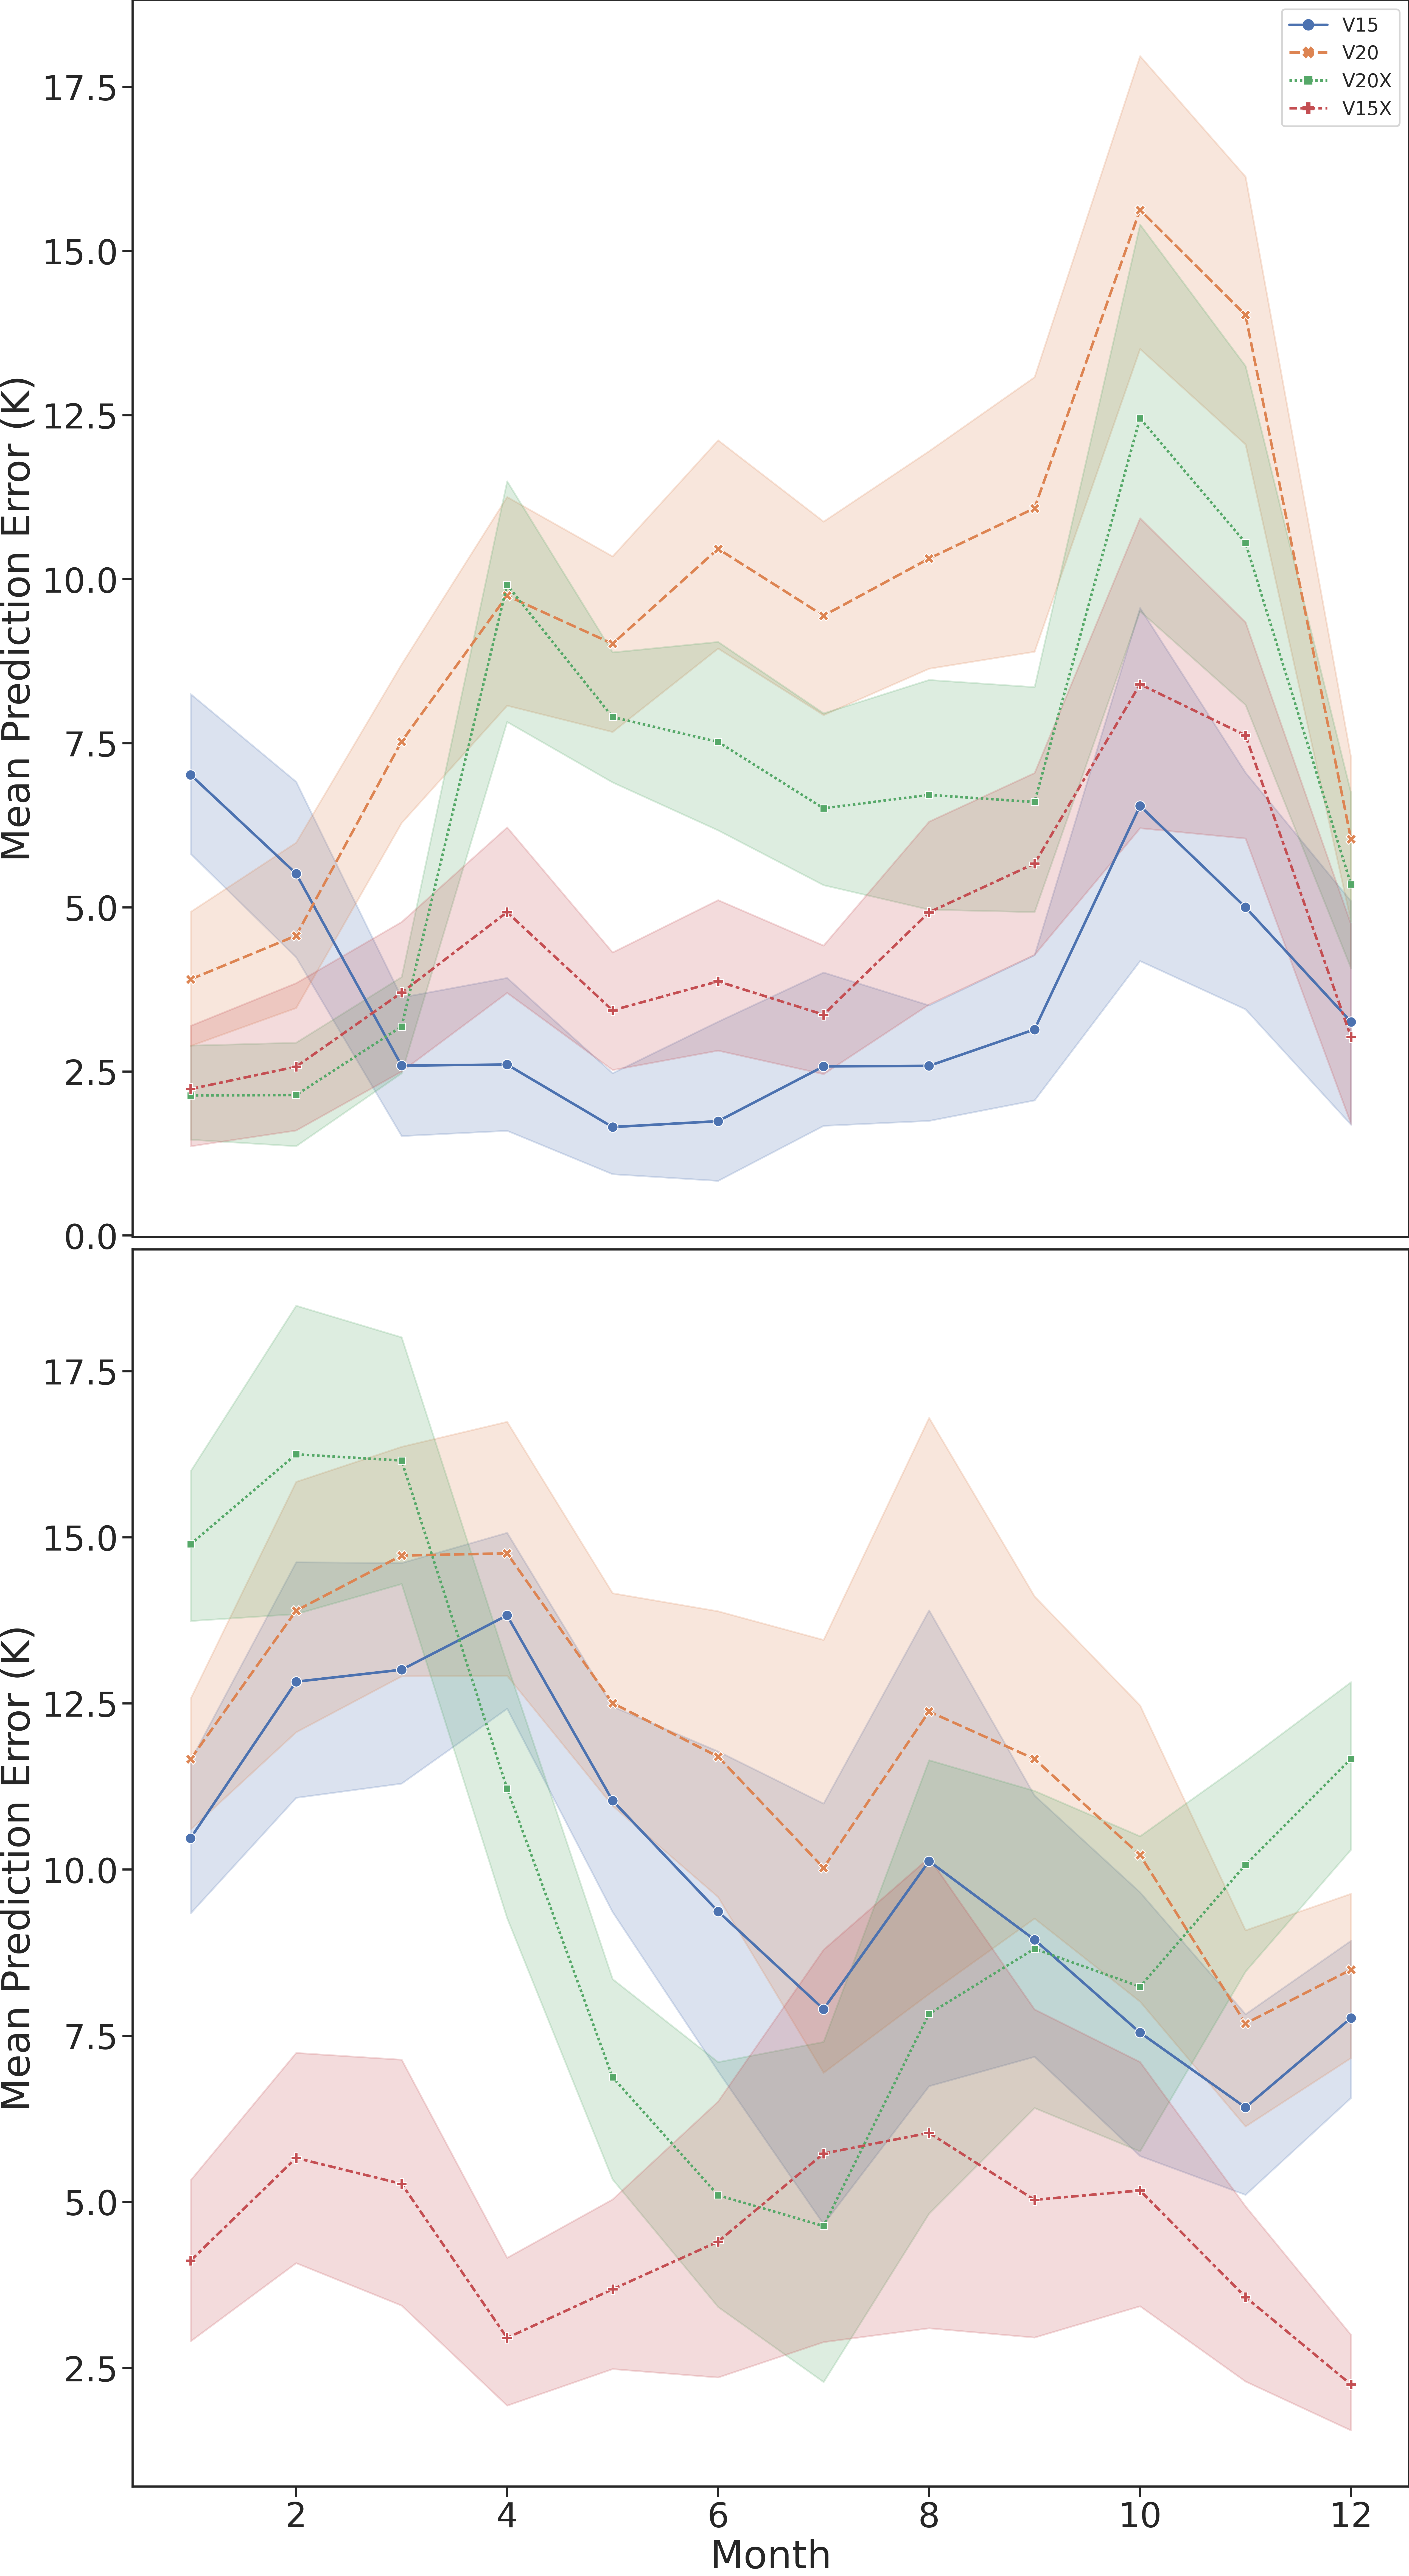
\includegraphics[width=\columnwidth]{stacked_timeseries_lakes_new.png}
%DIFDELCMD < 		%%%
\DIFdelendFL \DIFaddbeginFL 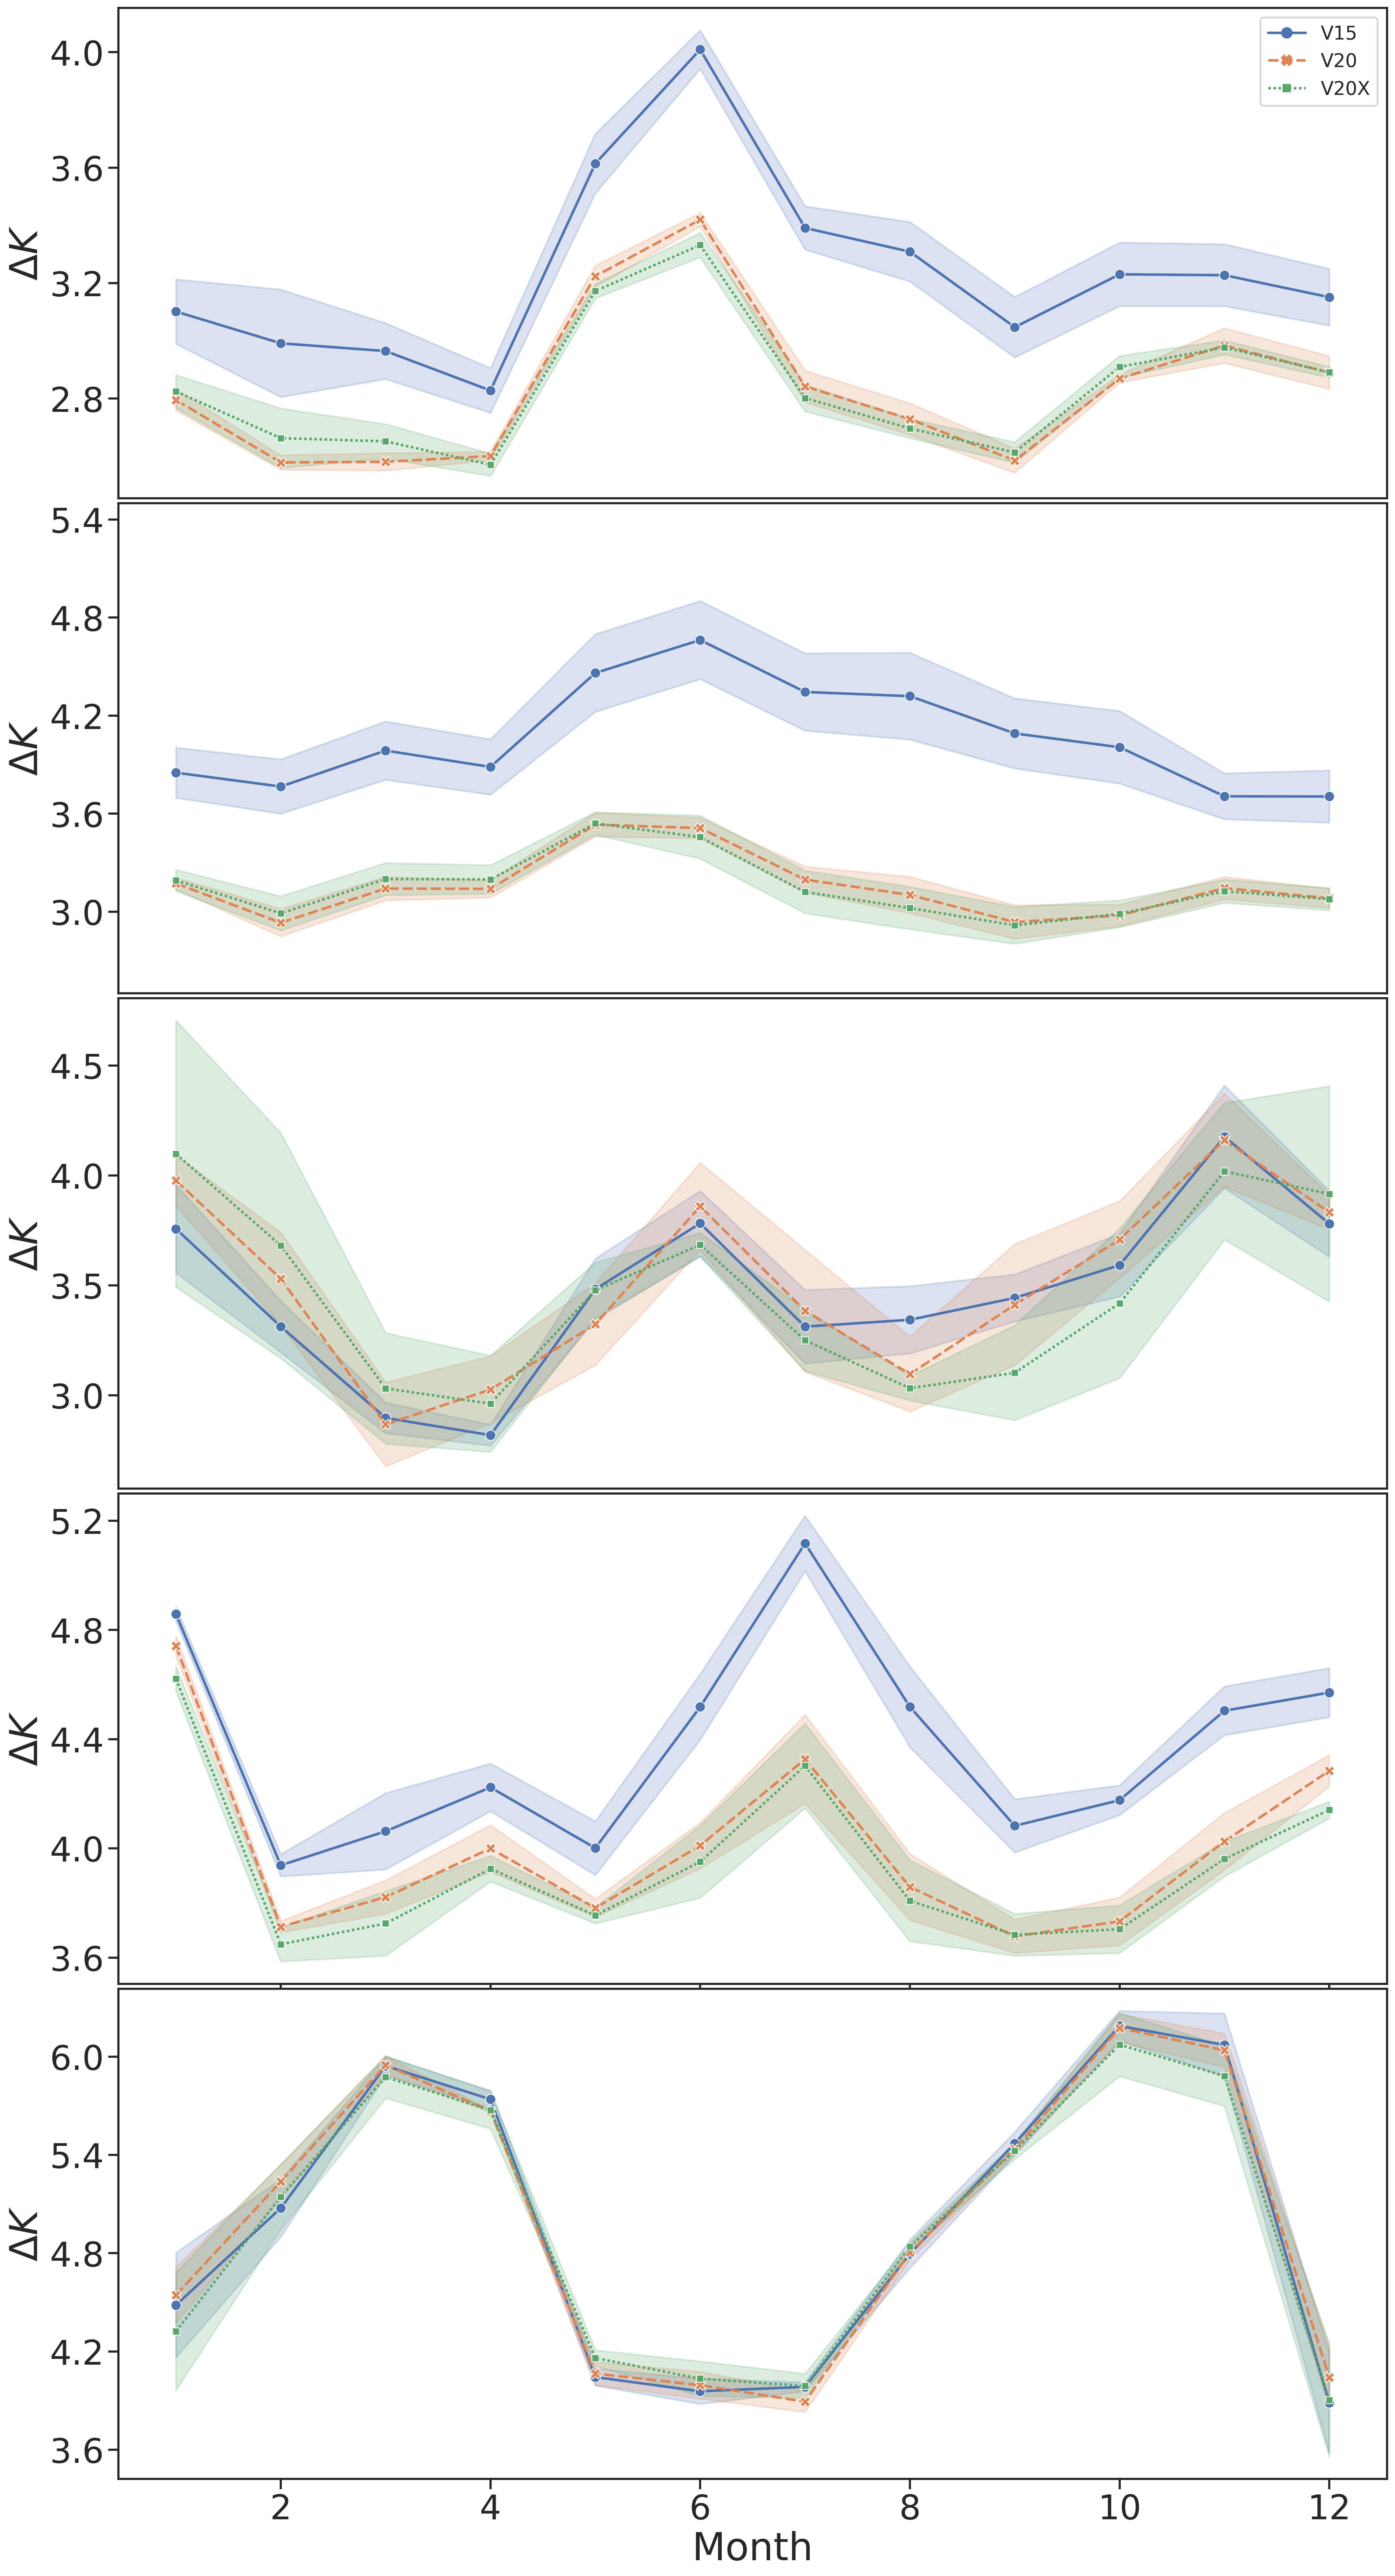
\includegraphics[scale=0.2]{new_timeseries_noise}
	\DIFaddendFL \caption{\DIFdelbeginFL \DIFdelFL{Variation in the }\DIFdelendFL \DIFaddbeginFL \DIFaddFL{Mean }\DIFaddendFL prediction error \DIFdelbeginFL \DIFdelFL{for }\DIFdelendFL \DIFaddbeginFL \DIFaddFL{in }\DIFaddendFL the \DIFaddbeginFL \DIFaddFL{surface temperature $Delta K$, averaged over all }\DIFaddendFL grid points\DIFdelbeginFL \DIFdelFL{at }\DIFdelendFL \DIFaddbeginFL \DIFaddFL{, for each of the 3 models over the course of the test year for (}\textit{\DIFaddFL{top panel}}\DIFaddFL{) }\DIFaddendFL Lake \DIFdelbeginFL \DIFdelFL{Natron}\DIFdelendFL \DIFaddbeginFL \DIFaddFL{Updates}\DIFaddendFL , \DIFdelbeginFL \DIFdelFL{Tanzania }\DIFdelendFL (\DIFdelbeginFL \DIFdelFL{top panel}\DIFdelendFL \DIFaddbeginFL \textit{\DIFaddFL{second panel}}\DIFaddendFL ) \DIFdelbeginFL \DIFdelFL{and Gujarat Province}\DIFdelendFL \DIFaddbeginFL \DIFaddFL{Lake-Ground Updates}\DIFaddendFL , \DIFdelbeginFL \DIFdelFL{India }\DIFdelendFL (\DIFdelbeginFL \DIFdelFL{bottom panel}\DIFdelendFL \DIFaddbeginFL \textit{\DIFaddFL{third panel}}\DIFaddendFL ) \DIFdelbeginFL \DIFdelFL{. There is a large degree of variability}\DIFdelendFL \DIFaddbeginFL \DIFaddFL{Vegetation Updates}\DIFaddendFL , \DIFdelbeginFL \DIFdelFL{but for }\DIFdelendFL \DIFaddbeginFL \DIFaddFL{(}\textit{\DIFaddFL{fourth panel}}\DIFaddFL{) Glacier Updates, northern hemisphere and (}\textit{\DIFaddFL{bottom panel}}\DIFaddFL{) Glacier Updates, southern hemisphere. The shaded regions show the $1 \sigma$ training noises. For the }\DIFaddendFL Lake \DIFdelbeginFL \DIFdelFL{Natron }\DIFdelendFL \DIFaddbeginFL \DIFaddFL{categories, all models follow }\DIFaddendFL the \DIFaddbeginFL \DIFaddFL{same general profile, with the VESPER\_}\DIFaddendFL V20 and \DIFaddbeginFL \DIFaddFL{VESPER\_}\DIFaddendFL V20X models \DIFdelbeginFL \DIFdelFL{are }\DIFdelendFL generally \DIFdelbeginFL \DIFdelFL{less performant than }\DIFdelendFL \DIFaddbeginFL \DIFaddFL{outperforming VESPER\_}\DIFaddendFL V15 \DIFdelbeginFL \DIFdelFL{and V15X, indicating that }\DIFdelendFL \DIFaddbeginFL \DIFaddFL{model over }\DIFaddendFL the \DIFdelbeginFL \DIFdelFL{updated V20 fields are less accurate here}\DIFdelendFL \DIFaddbeginFL \DIFaddFL{year}\DIFaddendFL .\DIFdelbeginFL \DIFdelFL{The augmented models with saline and monthly lake maps outperform those without, indicating the value of these fields in these regions.}\DIFdelendFL }
	\DIFaddbeginFL \label{fig:timeseries}
\end{figure}


	\begin{figure}
	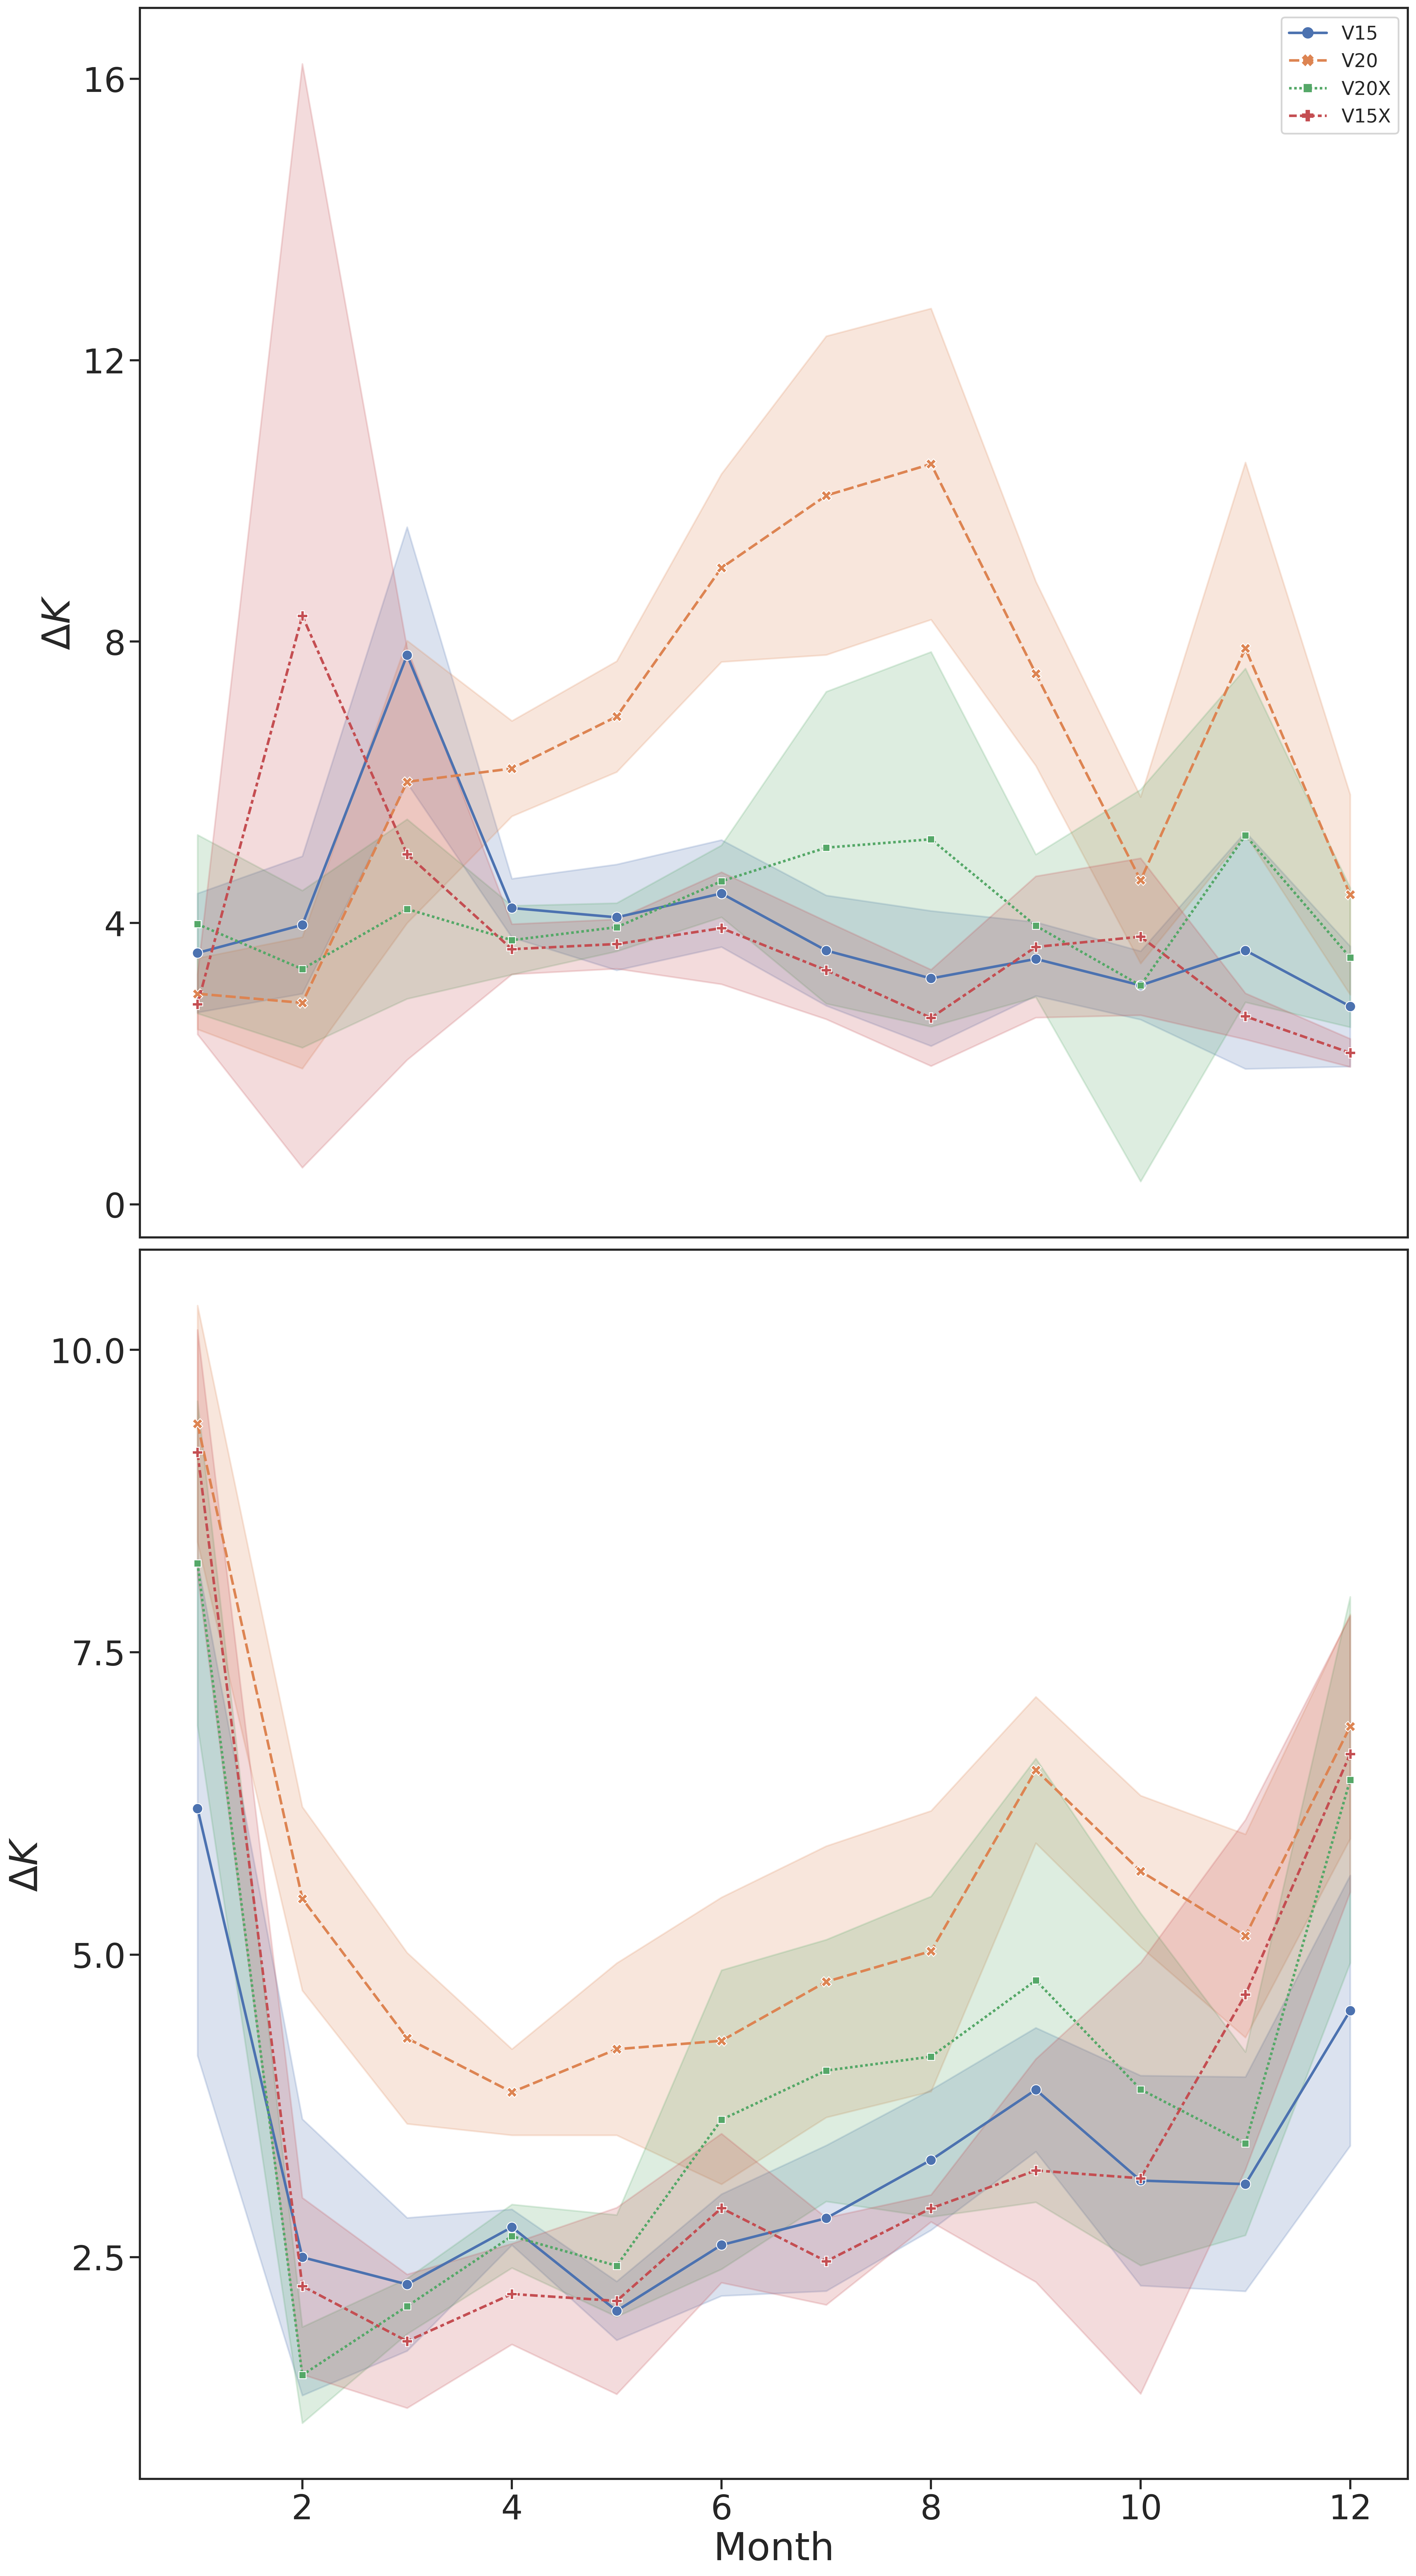
\includegraphics[scale=0.2]{timeseries_slc_chott}
	\caption{\DIFaddFL{Variation in the prediction error for the grid points at Great Salt Lake, Utah (top panel) and Chott Felrhir, Algeria (bottom panel). There is a large degree of variability, but for both grid points VESPER\_V20 model is generally less performant than VESPER\_V15 , indicating that the updated V20 fields are less accurate here. Corrections introduced by the augmented VESPER\_V20X model with saline and monthly lake maps outperform those without, indicating the value of these fields in these regions.The shaded regions show the $1 \sigma$ training noises.}} 
	\DIFaddendFL \label{fig:timeseries_stacked}
\end{figure}



\section{Discussion} \DIFdelbegin %DIFDELCMD < \label{sec:4}
%DIFDELCMD < 	%%%
\DIFdelend \DIFaddbegin \label{sec:discussion}
\DIFaddend We have seen how VESPER can quantitatively evaluate the value of updates to the lake surface parametrisation as well as identifying areas where the updates are \DIFdelbegin \DIFdel{insufficiently accurate}\DIFdelend \DIFaddbegin \DIFadd{inaccurate}\DIFaddend . For the former VESPER was able to show that the major regions where the lake surface parametrisation fields were updated - such as the Aral sea - enjoyed more accurate predictions, which verifies both the accuracy of the fields and their information content with respect to predicting skin temperatures. For the latter VESPER was able to identify grid points where the predictions became worse with the updated fields, indicating that the updated fields were in fact less accurate. More generally we have also seen how detailed knowledge of surface water fields (e.g. up to date permanent water distribution, seasonal water distribution, salt lake distribution, etc.) can notably improve the accuracy with which the skin temperature can be modelled, e.g. grid points with significant updates (i.e. where the field has changed by \DIFdelbegin \DIFdel{$\geq$ }\DIFdelend \DIFaddbegin \DIFadd{≥ }\DIFaddend 10 \%) to the lake fields show a mean absolute error reduction of skin temperature globally of \DIFdelbegin \DIFdel{$0.45$}\DIFdelend \DIFaddbegin \DIFadd{0.37}\DIFaddend K (Table \DIFdelbegin \DIFdel{\ref{tab:V1520_results}). }\DIFdelend \DIFaddbegin \DIFadd{\ref{tab:categorisation}). Given the performance of VESPER it may be possible in the future to update or correct the input fields at a high cadence, e.g. yearly or even more frequently.   }\newline 

\DIFaddend 


\DIFdelbegin %DIFDELCMD < \noindent %%%
\DIFdelend There are multiple possible further extensions of this work. We have not currently included the errors on the MODIS observations into the VESPER model. During the \DIFdelbegin \DIFdel{``}\DIFdelend \DIFaddbegin \DIFadd{“}\DIFaddend matching-in-space" step relating the ERA and MODIS data (Section \DIFdelbegin \DIFdel{\ref{sec:join}}\DIFdelend \DIFaddbegin \DIFadd{2.2}\DIFaddend ), it could be a worthwhile extension to weight the averaged MODIS points by their corresponding errors (e.g. Fig. \DIFdelbegin \DIFdel{\ref{fig:MODIS_obs_error}}\DIFdelend \DIFaddbegin \DIFadd{\ref{fig:modis_plot_2}}\DIFaddend ) when deriving a single MODIS observation for a given ERA grid point. This would then provide a more accurate and confident representation of the true surface temperature at a particular space-time point. Due to the inherent stochasticity of training a model \DIFdelbegin \DIFdel{it is also possible for different models to settle in different local minimas i. e. the network variance. It }\DIFdelend \DIFaddbegin \DIFadd{we have seen that some grid points have a particularly large training noise. To better quantify this effect and try to draw stronger conclusions for this subset of points it }\DIFaddend would also be desirable to train an ensemble of models (\DIFdelbegin \DIFdel{``}\DIFdelend \DIFaddbegin \DIFadd{“}\DIFaddend ensemble learning") and combine the predictions from multiple models to reduce this variance. \DIFaddbegin \DIFadd{Additionally, our examination of the value of the monthly lake maps is only a preliminary study. It would be of interest to follow seasonal lakes over a longer time period (e.g. decadal) beyond the 12 month maps that we use, in order to better quantify their time variability, as well as the differences between years (e.g. if the lake fraction was particularly high in the January of one year, but low in the subsequent year). It would also be of interest to try to quantify if VESPER and ECLand respond to changes in the input parametrisations in the same way, which is key to be able to then apply the VESPER results to the full earth system model development. Since VESPER is trained on ERA5, if we want to model the outputs of the IFS we must assume that the statistical behaviour of the input fields does not change from ERA to IFS. This is a fair assumption, but it would be interesting to investigate this quantitively in greater detail. }\DIFaddend We have focused here primarily on hydrological applications, our primary concern being the ability to evaluate the parametrised water body representation, however the \DIFdelbegin \DIFdel{method would work generally }\DIFdelend \DIFaddbegin \DIFadd{general application of the method }\DIFaddend for any updated fields that we want to assess \DIFaddbegin \DIFadd{could also be explored}\DIFaddend . Extension to non-lake hydrological fields like wetland \DIFdelbegin \DIFdel{extant }\DIFdelend \DIFaddbegin \DIFadd{extent }\DIFaddend or river bathymetry model parameters, or even non hydrological fields such as orography would be an interesting further development. The development of a more mature, integrated pipeline for automatically evaluating updated parametrisations could also be a worthwhile pursuit. \DIFdelbegin \DIFdel{Another natural }\DIFdelend \DIFaddbegin \newline 




\DIFadd{Another natural and interesting }\DIFaddend extension of this work \DIFaddbegin \DIFadd{would be to use VESPER to perform a feature importance or sensitivity analysis for the various input fields of the neural network. Additionally, an approach }\DIFaddend which may prove fruitful in the enterprise for improved parametrised representation of water bodies is to invert the problem and treat VESPER as a function to optimise. That is to say, VESPER can be thought of as a function which takes some inputs - in this case a lake parametrisation - and returns a loss metric i.e. how accurate the predictions are compared to the test set. Given this loss metric it may then be possible to vary the inputs and use standard optimisation techniques to learn the optimal parametrisation. Whilst this may be an expensive technique as there are effectively two nested models over which to optimise (for every optimisation step in the higher model, one must train the VESPER network from scratch) it could be possible given appropriate hardware or with reduced data focusing just on targeted locations (e.g. \DIFdelbegin \textit{\DIFdel{``What is the best way to represent the lakes in this area?"}}%DIFAUXCMD
\DIFdelend \DIFaddbegin \DIFadd{“What is the best way to represent the lakes in this area?"}\DIFaddend ). The loss gradient information can also be used to tune individual features, informing whether an input variable should be larger or smaller.




\section{Conclusion}\label{sec:conclusion}
Weather and climate modelling \DIFdelbegin \DIFdel{rely }\DIFdelend \DIFaddbegin \DIFadd{relies }\DIFaddend on accurate, up-to-date descriptions of surface fields, such as inland water, so as to provide appropriate boundary conditions for the numerical evolution. Lakes can significantly influence both weather and climate, but sufficiently  accurate  representation  of  lakes  is  challenging  and  the  natural  changes  in  water  bodies  mean  that  these representations  need  to  be  frequently  updated.  A  new  method  based  on  a  neural  network  regressor  for  automatically  and quickly verifying the updated lake fields - VESPER - has been presented in this work. This tool has been deployed to verify the recent updates to the FLake parametrisation, which include additional datasets such as the GSWE and updated methods for determining the lake depth from GLDBv3. The updated parametrisation fields were shown globally to be an improvement over the original fields; for a subset of grid points which have had significant updates to the lake fields, the prediction error in the skin temperature decreased by \DIFdelbegin \DIFdel{0.45}\DIFdelend \DIFaddbegin \DIFadd{a MAE of 0.37}\DIFaddend K. Conversely, VESPER also identified individual grid points where the updated lake fields were less accurate, enabling these points to subsequently be corrected, such as \DIFaddbegin \DIFadd{incorrect removal of lake water and }\DIFaddend losing forests to bare ground\DIFdelbegin \DIFdel{leading to errors of 1.1K}\DIFdelend . Multiple further extensions of this work, including extension to non lake fields and the development of a more mature integrated pipeline have been discussed.





\DIFdelbegin \section{\DIFdel{Code}}
%DIFAUXCMD
\addtocounter{section}{-1}%DIFAUXCMD
\DIFdel{The code used in constructing VESPER, including the methods for joining the ERA and MODIS datasets and the construction of the neural network regression model is open-sourced at }%DIFDELCMD < \url{https://github.com/tomkimpson/ML4L}
%DIFDELCMD < 	%%%
\DIFdelend \DIFaddbegin \clearpage
\newpage
\DIFadd{\mbox{~}

}\DIFaddend 





	
	


	

\DIFdelbegin \section{\DIFdel{Acknowledgments}}
	%DIFAUXCMD
\addtocounter{section}{-1}%DIFAUXCMD
\DIFdel{This project has received funding from the European Research Council (ERC) under the European Union’s Horizon 2020 research and innovation programme (Grant No 741112).
	}\DIFdelend %DIF > \section{Code}
\DIFaddbegin \codeavailability{The code used in constructing VESPER, including the methods for joining the ERA and MODIS datasets and the construction of the neural network regression model is open-sourced at \url{https://github.com/tomkimpson/ML4L}}

\DIFaddend 


%DIF > \section{Acknowledgments}

\DIFaddbegin 





\DIFaddend %\conclusions  %% \conclusions[modified heading if necessary]
%TEXT

%% The following commands are for the statements about the availability of data sets and/or software code corresponding to the manuscript.
%% It is strongly recommended to make use of these sections in case data sets and/or software code have been part of your research the article is based on.

%\codeavailability{TEXT} %% use this section when having only software code available


%\dataavailability{TEXT} %% use this section when having only data sets available


%\codedataavailability{TEXT} %% use this section when having data sets and software code available

%
%\sampleavailability{TEXT} %% use this section when having geoscientific samples available
%
%
%\videosupplement{TEXT} %% use this section when having video supplements available


%\appendix
%\section{}    %% Appendix A
%
%\subsection{}     %% Appendix A1, A2, etc.
%
%
%\noappendix       %% use this to mark the end of the appendix section. Otherwise the figures might be numbered incorrectly (e.g. 10 instead of 1).

%% Regarding figures and tables in appendices, the following two options are possible depending on your general handling of figures and tables in the manuscript environment:

%% Option 1: If you sorted all figures and tables into the sections of the text, please also sort the appendix figures and appendix tables into the respective appendix sections.
%% They will be correctly named automatically.

%% Option 2: If you put all figures after the reference list, please insert appendix tables and figures after the normal tables and figures.
%% To rename them correctly to A1, A2, etc., please add the following commands in front of them:

%\appendixfigures  %% needs to be added in front of appendix figures

%\appendixtables   %% needs to be added in front of appendix tables

%% Please add \clearpage between each table and/or figure. Further guidelines on figures and tables can be found below.



\DIFaddbegin \authorcontribution{All the authors contributed equally to the work.Tom Kimpson wrote the manuscript with contributions from all other authors.} %DIF > % this section is mandatory

\competinginterests{The authors declare that they have no conflict of interest.} %DIF > % this section is mandatory even if you declare that no competing interests are present

\DIFaddend %\disclaimer{TEXT} %% optional section

\DIFaddbegin \begin{acknowledgements}
\DIFadd{This project has received funding from the European Research Council (ERC) under the European Union’s Horizon 2020 research and innovation programme (Grant No 741112). PD gratefully acknowledges funding from the ESiWACE project funded under Horizon 2020 No. 823988. PD and MC gratefully acknowledge funding from the MAELSTROM EuroHPC-JU project (JU) under No 955513. The JU receives support from the European Union’s Horizon research and innovation programme and United Kingdom, Germany, Italy, Luxembourg, Switzerland, and Norway.

}

\end{acknowledgements}




\DIFaddend %% REFERENCES

\DIFdelbegin %DIFDELCMD < \newpage
%DIFDELCMD < %%%
%DIF < %%%%%%%%%%%%%%%%%%%%%%%%%
%DIF < BIBLIOGRAPHY
%DIFDELCMD < \bibliographystyle{ieeetr}
%DIFDELCMD < \bibliography{refs}
%DIFDELCMD < %%%
%DIF < \begin{thebibliography}{refs}
%DIF < \bibitem{}
\DIFdelend %DIF > % The reference list is compiled as follows:

\DIFaddbegin 

%DIF > \begin{thebibliography}{}
%DIF > 
%DIF > \bibitem[AUTHOR(YEAR)]{LABEL1}
%DIF > REFERENCE 1
%DIF > 
%DIF > \bibitem[AUTHOR(YEAR)]{LABEL2}
%DIF > REFERENCE 2
%DIF > 
\DIFaddend %\end{thebibliography}

\DIFaddbegin 

%DIF > % Since the Copernicus LaTeX package includes the BibTeX style file copernicus.bst,
%DIF > % authors experienced with BibTeX only have to include the following two lines:
%DIF > %
 \bibliographystyle{copernicus}
 \bibliography{refs.bib}
%DIF > %
%DIF > % URLs and DOIs can be entered in your BibTeX file as:
%DIF > %
%DIF > % URL = {http://www.xyz.org/~jones/idx_g.htm}
%DIF > % DOI = {10.5194/xyz}


%DIF > % LITERATURE CITATIONS
%DIF > %
%DIF > % command                        & example result
%DIF > % \citet{jones90}|               & Jones et al. (1990)
%DIF > % \citep{jones90}|               & (Jones et al., 1990)
%DIF > % \citep{jones90,jones93}|       & (Jones et al., 1990, 1993)
%DIF > % \citep[p.~32]{jones90}|        & (Jones et al., 1990, p.~32)
%DIF > % \citep[e.g.,][]{jones90}|      & (e.g., Jones et al., 1990)
%DIF > % \citep[e.g.,][p.~32]{jones90}| & (e.g., Jones et al., 1990, p.~32)
%DIF > % \citeauthor{jones90}|          & Jones et al.
%DIF > % \citeyear{jones90}|            & 1990



%DIF > % FIGURES

%DIF > % When figures and tables are placed at the end of the MS (article in one-column style), please add \clearpage
%DIF > % between bibliography and first table and/or figure as well as between each table and/or figure.

%DIF >  The figure files should be labelled correctly with Arabic numerals (e.g. fig01.jpg, fig02.png).


%DIF > % ONE-COLUMN FIGURES

%DIF > %f
%DIF > \begin{figure}[t]
%DIF > \includegraphics[width=8.3cm]{FILE NAME}
%DIF > \caption{TEXT}
%DIF > \end{figure}
%DIF > 
%DIF > %% TWO-COLUMN FIGURES
%DIF > 
%DIF > %f
%DIF > \begin{figure*}[t]
%DIF > \includegraphics[width=12cm]{FILE NAME}
%DIF > \caption{TEXT}
%DIF > \end{figure*}
%DIF > 
%DIF > 
%DIF > %% TABLES
%DIF > %%
%DIF > %% The different columns must be seperated with a & command and should
%DIF > %% end with \\ to identify the column brake.
%DIF > 
%DIF > %% ONE-COLUMN TABLE
%DIF > 
%DIF > %t
%DIF > \begin{table}[t]
%DIF > \caption{TEXT}
%DIF > \begin{tabular}{column = lcr}
%DIF > \tophline
%DIF > 
%DIF > \middlehline
%DIF > 
%DIF > \bottomhline
%DIF > \end{tabular}
%DIF > \belowtable{} % Table Footnotes
%DIF > \end{table}
%DIF > 
%DIF > %% TWO-COLUMN TABLE
%DIF > 
%DIF > %t
%DIF > \begin{table*}[t]
%DIF > \caption{TEXT}
%DIF > \begin{tabular}{column = lcr}
%DIF > \tophline
%DIF > 
%DIF > \middlehline
%DIF > 
%DIF > \bottomhline
%DIF > \end{tabular}
%DIF > \belowtable{} % Table Footnotes
%DIF > \end{table*}
%DIF > 
%DIF > %% LANDSCAPE TABLE
%DIF > 
%DIF > %t
%DIF > \begin{sidewaystable*}[t]
%DIF > \caption{TEXT}
%DIF > \begin{tabular}{column = lcr}
%DIF > \tophline
%DIF > 
%DIF > \middlehline
%DIF > 
%DIF > \bottomhline
%DIF > \end{tabular}
%DIF > \belowtable{} % Table Footnotes
%DIF > \end{sidewaystable*}
%DIF > 
%DIF > 
%DIF > %% MATHEMATICAL EXPRESSIONS
%DIF > 
%DIF > %% All papers typeset by Copernicus Publications follow the math typesetting regulations
%DIF > %% given by the IUPAC Green Book (IUPAC: Quantities, Units and Symbols in Physical Chemistry,
%DIF > %% 2nd Edn., Blackwell Science, available at: http://old.iupac.org/publications/books/gbook/green_book_2ed.pdf, 1993).
%DIF > %%
%DIF > %% Physical quantities/variables are typeset in italic font (t for time, T for Temperature)
%DIF > %% Indices which are not defined are typeset in italic font (x, y, z, a, b, c)
%DIF > %% Items/objects which are defined are typeset in roman font (Car A, Car B)
%DIF > %% Descriptions/specifications which are defined by itself are typeset in roman font (abs, rel, ref, tot, net, ice)
%DIF > %% Abbreviations from 2 letters are typeset in roman font (RH, LAI)
%DIF > %% Vectors are identified in bold italic font using \vec{x}
%DIF > %% Matrices are identified in bold roman font
%DIF > %% Multiplication signs are typeset using the LaTeX commands \times (for vector products, grids, and exponential notations) or \cdot
%DIF > %% The character * should not be applied as mutliplication sign
%DIF > 
%DIF > 
%DIF > %% EQUATIONS
%DIF > 
%DIF > %% Single-row equation
%DIF > 
%DIF > \begin{equation}
%DIF > 
%DIF > \end{equation}
%DIF > 
%DIF > %% Multiline equation
%DIF > 
%DIF > \begin{align}
%DIF > & 3 + 5 = 8\\
%DIF > & 3 + 5 = 8\\
%DIF > & 3 + 5 = 8
%DIF > \end{align}
%DIF > 
%DIF > 
%DIF > %% MATRICES
%DIF > 
%DIF > \begin{matrix}
%DIF > x & y & z\\
%DIF > x & y & z\\
%DIF > x & y & z\\
%DIF > \end{matrix}
%DIF > 
%DIF > 
%DIF > %% ALGORITHM
%DIF > 
%DIF > \begin{algorithm}
%DIF > \caption{...}
%DIF > \label{a1}
%DIF > \begin{algorithmic}
%DIF > ...
%DIF > \end{algorithmic}
%DIF > \end{algorithm}
%DIF > 
%DIF > 
%DIF > %% CHEMICAL FORMULAS AND REACTIONS
%DIF > 
%DIF > %% For formulas embedded in the text, please use \chem{}
%DIF > 
%DIF > %% The reaction environment creates labels including the letter R, i.e. (R1), (R2), etc.
%DIF > 
%DIF > \begin{reaction}
%DIF > %% \rightarrow should be used for normal (one-way) chemical reactions
%DIF > %% \rightleftharpoons should be used for equilibria
%DIF > %% \leftrightarrow should be used for resonance structures
%DIF > \end{reaction}
%DIF > 
%DIF > 
%DIF > %% PHYSICAL UNITS
%DIF > %%
%DIF > %% Please use \unit{} and apply the exponential notation

\DIFaddend 


\end{document}
